\documentclass[11pt,a4paper]{report}

\usepackage[utf8]{inputenc}
\usepackage[T1]{fontenc}
\usepackage{amsmath,amssymb,amsthm,mathtools}
\usepackage{booktabs}
\usepackage{hyperref}
\usepackage{cleveref}
\usepackage[margin=1in]{geometry}
\usepackage{graphicx}
\usepackage{subcaption}
\usepackage{placeins}
\usepackage{float}
\usepackage{siunitx}
\usepackage{longtable}
\usepackage{lmodern}
\usepackage{microtype}
\usepackage{enumitem}
\usepackage{xcolor}
\usepackage{hyperref}
\usepackage{lipsum}
\usepackage[backend=biber]{biblatex}

\addbibresource{references2.bib}

\newtheorem{assumption}{Assumption}
\newtheorem{definition}{Definition}
\newtheorem{theorem}{Theorem}
\newtheorem{proposition}{Proposition}
\newtheorem{corollary}{Corollary}
\newtheorem{remark}{Remark}
\newtheorem{lemma}{Lemma}
\newcommand{\dd}{\,\mathrm d}
\newcommand{\Dcol}{D_{\mathrm{col}}}
\newcommand{\Dself}{D_{\mathrm{self}}}
\newcommand{\Dn}{D_n}
\newcommand{\rhojam}{\rho_{\mathrm{jam}}}
\newcommand{\phijam}{\Phi_{\mathrm{jam}}}
\newcommand{\pjam}{p_{\mathrm{jam}}}
\newcommand{\njam}{n_{\mathrm{jam}}}
\newcommand{\Ljam}{L_{\mathrm{jam}}}
\newcommand{\Lre}{L_{\mathrm{re}}}
\newcommand{\ellstarv}{\ell_{\mathrm{s}}}
\newcommand{\Psiinv}{\Psi^{-1}}



\newcommand{\pd}{\partial}
\newcommand{\R}{\mathbb R}
\newcommand{\one}{\mathbf 1}
\newcommand{\diag}{\operatorname{diag}}
\newcommand{\sgn}{\operatorname{sgn}}
\newcommand{\atanh}{\operatorname{artanh}}
\newcommand{\E}{\mathcal E}
\newcommand{\Kop}{\mathcal K}
\newcommand{\Lop}{\mathcal L}
\newcommand{\Pmat}{\mathsf P}
\newcommand{\Kmat}{\mathsf K}
\newcommand{\Id}{\mathsf I}
\newcommand{\q}{q}
\newcommand{\h}{h}
%probably will write it in a way where it isnt a theorem-proof style, but leaving it in for now

\begin{document}
		\begin{titlepage}
			\centering
			
			\vspace*{2cm}
			
			{\LARGE\bfseries Nutrient-Limited Dynamics in Confined Cavities\par}
			
			\vspace{1.5cm}
			
			{\Large Bachelor's Thesis\par}
			
			\vfill
			
			{\large
				Author: Paul Tizian Spitznagel
			}
			
			\vspace{2cm}
			
			\begin{flushleft}
				\begin{tabular}{@{}ll}
					Submitted to:     & Leipzig University \\
					& Faculty of Physics and Earth System Sciences \\
					Institute:        & Peter Debye Institute for Soft Matter Physics \\
					Division:         & Statistical Physics of Evolution  \\
					Supervisors:    & Valentin Slepukhin, Ralf Steuer \\
					First Examiner:   & Professor Ralf Steuer \\
					Second Examiner:  & Valentin Slepukhin PhD \\
					Date:             & \today
				\end{tabular}
			\end{flushleft}
			
			\vfill

		
	\end{titlepage}
	\chapter*{Abstract}
	How bacteria form colonies in confined cavities has previously been studied in nutrient rich conditions, we extend this to make analytical and numerical prediction about strain phase transitions and sorting in resource competition under nutrient limitation. We show that the jamming transition, previously known to be abrupt \cite{Karita}, is continuous if it has barely enough nutrients to reach this state. Additionally we give a numerically validated threshold length formula, relating endpoint nutrient concentration and cavity length. When two strains compete for the same limited nutrient they do not simply sort to their advantage, we found that they can dominate regions where they are locally disfavored which we call inverse sorting. This can be either transient with Tilmans $R^*$ \cite{rstar} limit for the dilute cavity or permanent over a cells lifespan if the population becomes jammed. This suggests that taking a snapshot of a composition is not reflective of the strains specialty niche. We demonstrate that even a simple deterministic reaction-diffusion model is capable of producing interesting results.\\
	\\
	Die Formung von bakteriellen Kolonien in Kavitäten wurde bisher nur in nährstoffreichen Zuständen ausgiebig erforscht, wir erweitern dies um die Limitierung der Nährstoffe der Zellen mittels analytischer und numerischer Prognosen in Phasenübergängen und räumlicher Sortierung bei Ressourcenkonkurrenz. Wir zeigen, dass der Übergang in den verklemmten Zustand, welcher bisher als abrupt galt \cite{Karita}, unter limitierter Nahrung stetig werden kann. Zudem ist ein Hauptpunkt der Gleichgewichtszustandsanalyse die numerisch validierte Schwellenlänge, die Kavitätenlänge und Nahrungskonzentration am Endpunkt direkt miteinander in Verbindung setzt. Wenn zwei Bakterienstämme um die gleiche Nahrung konkurrieren sortieren sie sich nicht räumlich nach ihrem lokalen Vorteil, sondern sie können sich fast komplett ihrem nach Zelleigenschaft bedingtem Wachstumsvorteil entgegen sortieren. Diese inverse Sortierung kann entweder, wie im gasförmigen Zustand, zeitlich vorübergehend sein, mit dem Gewinner des Wettkampfs nach Tilmans $R^*$ Regel \cite{rstar} oder über dem Lebenszeitraum einer Zelle permanent einfrieren. Dies suggeriert, dass man aus einer Zeitpunktaufnahme der räumlichen Zellenverteilung nicht auf Zelleneigenschaften schließen kann, sondern die Sortierung ein Produkt aus historischer Selektion und Advektion ist. Wir demonstrieren, dass selbst ein simpel gehaltenes Reaktions-Diffusions Modell dazu fähig ist interessante Ergebnisse zu produzieren.
	\tableofcontents
	\chapter{Introduction}
	Bacterial cells can form colonies in many different geometries, a common habitat for them are spatially confined cavities. These microhabitats could for example be soil pores, gut crypts or tooth cavities in carious lesions \cite{Karita} \cite{tooth}. Microbes inside a confined cavity of lengths $10-350 \mathrm{\mu m}$ are very stable, reaching a steady state within a couple days of running the experiment \cite{Karita}. Whether this steady state is empty, dilute or jammed was found to be heavily length dependent. However the experiments were explicitly nutrient rich, as such nutrient limitation and the accompanying dynamics were left unconsidered. We aim to investigate how nutrient limitation changes length-dependent population dynamics and state transitions. We extend a model of the experimental device called "Microfluidic Panflute" used by Karita \cite{Karita} which confines bacteria inside crypt shaped chambers. Multiple cavities of varying lengths are ordered by length next to each other with an orthogonal flow supplying the bacteria needed for colonization which enter through the opening. The flow at the opening  simultaneously functions as a washout for cells, if cells from the inside reach the opening the flow carries them out of the cavity. Food only enters through the same channel,  as such the opening is a death trap for greedy cells, if they chase the nutrient gradient too strongly they cannot colonize the cavity as they get washed out of their prospective habitat. This would be an important mechanism for nutrient chasing chemotaxis, which remains beyond the scope of this thesis. We simulate E. coli strains consuming glucose to grow and investigate how nutrient limitation changes phase state transitions and spatial pattern formation. The E. coli bacterium has been studied for decades and as such a large amount of experimental data has accumulated over the years, making it a standard parameter reference for modeling cells in microbial communities. Equivalently glucose is a common nutrient source for bacterial strains, specifically as a carbon and energy source for our E. coli strains. In spatial models resource competition inherently leads to pattern formation, sorting, exclusion or coexistence. For example the introduction of small defects at the floor can make strains sort themselves into their own regions over time, rescuing the slower strain from its death \cite{slepukhin}. A common limited resource competition prediction is the R* rule, which expects the population which can survive and grow better at lower nutrient availability to eventually take over. When two populations compete for the same nutrient, it is rarely observed in nature that they can coexist \cite{Murray}. However the introduction of spatial structure can create stable coexistence in competing populations by finding their own niche if they have a trade-off\cite{Tilman}. In Tilmans model the trade-off lies in differing colonization and competition rates, while in our model it lays in the nutrient dependent growth functions. Another example of coexistence are the anolis lizards of bimini, here 4 different species of lizards live in the same forest however are broadly divided into different sub regions, based on perch height and diameter preference \cite{lizard}. All of them feed mostly on the same ants, while each species is better suited for colonization in different regions of the forest, making them specialists. As such they sort according to their local advantage even though their food is globally present in the broad region. One could similarly assume that this would also apply for our specialist E. coli strains, expecting each strain to simply sort to where they have the advantage. The high affinity strain as such would mostly occupy the nutrient depleted interior and dead end while the glutton would dominate the nutrient rich opening. However perch heights in the lizard population sorting is static in space and time, our growth advantages are spatiotemporal as they change depending on the nutrient concentration. We found the sorting is not simply dominated by the local environment, in fact strains can dominate regions completely where they are locally disfavored. Making the sorting between strains inherently dependent on the history of selection and advection. Whether one strain wins or they end up being able to coexist depends heavily on the population state, i.e. if the community is jammed or dilute.
	\chapter{Model}
	\label{model}
	\section{Microbial communities inside cavities}
	We consider a one dimensional dead end cavity on
	\begin{equation}
		x\in[0,L].
	\end{equation}
	with
	\begin{equation}
		x=0 \quad \text{opening},
		\qquad
		x=L \quad \text{bottom/closed end}.
	\end{equation}
	As such $L$ denotes the length of the cavity. The biomass density is the volume fraction occupied by cells
	\begin{equation}
		\rho=\rho(x,t)\in[0,1]
	\end{equation}
	In our idealized model no cells can be present at the opening, yielding the boundary condition of density $\rho(0,t)=0$. Nutrients are steadily supplied through the opening, set by nutrient concentration $n(0,t)=n_0$, making it the only continuous supply of food for the cells. Analogous to the Panflute model \cite{Karita}, we use the no flux condition at the closed end $J(L,t)=0$. Using Fick's first law of diffusion $J=-D\frac{d\phi}{dx}$, with the substrate concentration $\phi$ and diffusion $D$ \cite{Fick}, the no flux condition is equivalent to our two concentration gradients $n_x (L,t)=0$ and $\rho_x (L,t)=0$ making our system bounded by Dirichlet and Neumann boundary conditions \cite{Leveque}.
	We work inside a one dimensional continuum model without considering individual cells, as such parameters from our model base \cite{Karita} \cite{slepukhin} require translation. The packing fraction $\Phi$ is defined in 3D as $\Phi=\rho V_{\rm cell}$ \cite{Karita} and in 2D as $\Phi=\rho A_{\rm cell}$ \cite{slepukhin} with a jamming transition at $\Phi_{\rm jam}=0.64$. So in their models the packing fraction and density are two separate variables. In a 1D continuum however it is opportune to choose $\Phi=\rho$, making the biomass density nondimensional and a cross section average. This convention allows us to eliminate cell size from the model completely while retaining the transport closures, since crowding depends on the amount of space occupied and not how many cells that fraction is divided into.\\
	\\
	Most notably we introduce nutrient limitation, with the concentration of nutrient given by
	\begin{equation}
		n=n(x,t)\ge 0.
	\end{equation}
	As such growth now depends on available nutrients and is a position and time dependent function of $n$ rather than constant as in previous models \cite{Karita}. The main simulations consider a cavity length of $L=1000 \mathrm{\mu m}$, as a very long cavity of 1mm allows for more extreme spatial effects.

\subsection{Governing equations for one strain}
\paragraph{Full nutrient coupled continuum model}
\label{sec:full_model_new}

Building on the general continuity equations of Karita \& Slepukhin \cite{Karita}\cite{slepukhin}. The biomass balance is
\begin{equation}
	\partial_t\rho+\partial_xJ_\rho=g(n)\rho,
	\qquad
	J_\rho=-D_{\rm col}(\rho)\rho_x.
	\label{eq:rho_flux_balance}
\end{equation}
\begin{equation}
	{
		\partial_t\rho
		=\partial_x\left(D_{\rm col}(\rho)\rho_x\right)+g(n)\rho.
	}
	\label{eq:rho_pde_new}
\end{equation}
and the nutrient balance with Monod growth and a nutrient sink \cite{Monod}
\begin{equation}
	\partial_t n+\partial_xJ_n=-\frac{1}{Y}g(n)\rho,
	\qquad
	J_n=-D_n n_x,
\end{equation}

\begin{equation}
	{
		\partial_t n=D_n n_{xx}-\frac{1}{Y}g(n)\rho.
	}
	\label{eq:n_pde_new}
\end{equation}



\paragraph{Steady state problem}
\label{sec:steady_problem}

Assuming a steady state gives us
\begin{equation}
	{
		\partial_x\left(D_{\rm col}(\rho)\rho_x\right)+g(n)\rho=0,
	}
	\label{eq:steady_rho_new}
\end{equation}
\begin{equation}
	{
		D_n n_{xx}=\frac{1}{Y}g(n)\rho.
	}
	\label{eq:steady_n_new}
\end{equation}
The steady state boundary conditions are
\begin{equation}
	{
		\rho(0)=0,
		\qquad
		n(0)=n_0,
		\qquad
		J_\rho(L)=0,
		\qquad
		n_x(L)=0.
	}
	\label{eq:steady_bcs_new}
\end{equation}
\subsection{Resource competition}	
We consider two strain densities individually as $\rho_1(x,t), \rho_2(x,t)$ with the total biomass packing fraction $\rho(x,t)=\rho_1(x,t)+\rho_2(x,t)$. For $\rho>0$ define the strain 1 fraction $f(x,t)=\frac{\rho_1(x,t)}{\rho(x,t)}$
and the centered dominance variable $h(x,t)=2f(x,t)-1$.
So
\begin{equation}
	h>0 \Longleftrightarrow f>\frac{1}{2} \Longleftrightarrow \rho_1>\rho_2,
	\qquad
	h<0 \Longleftrightarrow f<\frac{1}{2} \Longleftrightarrow \rho_2>\rho_1.
\end{equation}
As such for equally seeded strains, the initial condition is $f_0=\frac{1}{2}$ or $h_0=0$.
\paragraph{Fluxes and transport}	
The two strains share a total biomass flux \(J\), but also undergo relative self diffusion.\cite{Karita}
\begin{align}
	J_1 &= fJ-\Dself(\rho)\rho\,\pd_x f,
	\label{eq:J1}\\
	J_2 &= (1-f)J+\Dself(\rho)\rho\,\pd_x f.
	\label{eq:J2}
\end{align}
\begin{equation}
	J_1+J_2=J.
\end{equation}
The total flux is collective diffusion down the total density gradient \cite{Karita} \cite{slepukhin} \cite{Fick}
\begin{equation}
	J=-\Dcol(\rho)\pd_x\rho.
	\label{eq:total-J}
\end{equation}
\paragraph{Continuity equations and boundary conditions}
The strain equations are
\begin{align}
	\pd_t\rho_1+\pd_xJ_1 &= g_1(n)\rho_1,
	\label{eq:rho1-eq}\\
	\pd_t\rho_2+\pd_xJ_2 &= g_2(n)\rho_2.
	\label{eq:rho2-eq}
\end{align}
The nutrient equation is
\begin{equation}
	\pd_t n=D_n\pd_{xx}n-\frac1Y\left[g_1(n)\rho_1+g_2(n)\rho_2\right].
	\label{eq:nutrient-eq}
\end{equation}
The cavity boundary conditions are
\begin{equation}
	n(0,t)=n_0,
	\qquad
	\pd_x n(L,t)=0,
	\label{eq:nutrient-bc}
\end{equation}
\begin{equation}
	\rho(0,t)=0,
	\qquad
	J(L,t)=0.
	\label{eq:biomass-bc}
\end{equation}
For the relative self diffusion term the boundary condition is no relative flux:
\begin{equation}
	\Dself(\rho)\rho\pd_x f=0
	\quad\text{at }x=0,L.
	\label{eq:relative-bc}
\end{equation}
	\section{Escherichia coli strains consuming Glucose} 
	\label{sec:ecoli} 
	\paragraph{Monod Parameters}
	Maximum growth rates for several E. coli mutant strains in sugar have been extensively measured by Steinsiek \& Bettenbrock \cite{Steinsiek}, we model K12 MG1655 strains and its genetic derivatives. The isogenic ptsG mutant has a maximum growth rate of $\mu_{1}=0.21 \mathrm{h^{-1}}$ while its parent MG1655 was measured to possess a maximum growth rate of $\mu_{2}=0.78\mathrm{h^{-1}}$ at full saturation. Assuming crossing growth functions set by sufficiently differing half-velocity constants $K$ in the Monod growth law makes the parent a glutton and the ptsG mutant the scavenger in their relationship as they compete for the same glucose nutrient source. The Monod constants $K$ however have not been measured directly in this paper, so the classification of glutton vs scavenger remains a design choice rather than being directly biologically grounded in their experiments. We choose the Monod constants $K_{1}=0.2 \mathrm{\mu M}$ and $K_{2}=15 \mathrm{\mu M}$ to design the crossover.
	\paragraph{Yield}
	The Yield coefficient, more generally, is the weight of bacteria formed by the weight of nutrient consumed \cite{Murray2}. As such it is inherently coupled to a cells growth rate, marking how much E. coli biomass has grown from the amount of glucose that was eaten. For E. coli in glucose the yield has been measured as $Y_{X/S}=0.45 \pm 0.03\ \mathrm{g(DW)\cdot g(sugar)^{-1}}$ by Lendenmann \cite{Lendenmann}. To fit our model this needs to be rescaled to biomass density or packing fraction per $\mu M$, so $Y=\frac{Y_{X/S}M}{\rho_{dry}} \times 10^{-6}\mathrm{\mu M^{-1}}=2.895 \times 10^{-7}\mathrm{\mu M^{-1}}$ with the molar mass of glucose $M=180.16 \mathrm{g/mol}$ and E. coli dry mass $\rho_{dry}=280 \mathrm{g/L}$.
	%https://bionumbers.hms.harvard.edu/bionumber.aspx?id=103904&ver=17 probably needs a different source, dry mass. Value is under the assumption of cell size 1 um^3
	%https://en.wikipedia.org/wiki/Glucose, glucose molar mass
	\paragraph{Nutrient diffusivity}
	How fast nutrients diffuse would normally depend on biomass density, however for simplicity's sake we assume it to be constant. For our nutrient glucose, the diffusion constant of it in water is given by Stewart \cite{stewart} at $25\,^\circ\mathrm{C}$ as $D_n=6.7 \times 10^{-6}  \mathrm{cm^2/s}=2.4 \times 10^6 \mathrm{\mu m^2/h}$. An additional factor can typically vary between 0.2 and 0.8 depending on the population state in biofilm, as such we take the average for our cavity and use $D_n=1.2 \times 10^6 \mathrm{\mu m^2/h}$.
	
	\chapter{Results}
	
	\section{Microbial single strain populations in steady state}
	\subsection{Invariant}
	\label{sec:invariant_new}
	\paragraph{Pressure potential in the density variable}
	\label{sec:pressure_potential_new}
	We define the pressure potential, as in \cite{Karita} \cite{slepukhin}
	\begin{equation}
		{
			\Psi(\rho)=\int_0^\rho D_{\rm col}(s)\,ds.
		}
		\label{eq:Psi_def_new}
	\end{equation}
	which allows us to rewrite the governing equation of our system as one invariant \cref{invariant}
	\begin{equation}
		{
			\Psi(\rho(x))+YD_n n(x)=YD_n n_0.
		}
		\label{eq:level_set_zero_opening}
	\end{equation}
It holds to numerical precision with a residual of $10^{-16}$ \ref{fig:steadyclosures}.
	\subsection{Pressure-plane reduction}
	\label{sec:pressure_plane_new}
	We can now define the effective depletion threshold $n_*\in(0,n_0)$ and accordingly $\rho_*=\Psi^{-1}(YD_n(n_0-n_*))$ with the corresponding effective depletion length $L_*:=\inf\{L>0:\ n(L;L)=n_*\}$. Here $n(x; L)$ is the steady state nutrient profile in a cavity with length $L$ and we evaluate it at the closed end $x = L$. The general formula without approximations is \ref{plane}
	\begin{equation}
		{
			L_*=
			\int_0^{p_*}
			\frac{dp}{\sqrt{2\int_p^{p_*}g(n(s))\rho(s)\,ds}}.
		}
	\end{equation}
\begin{figure}
	\centering
	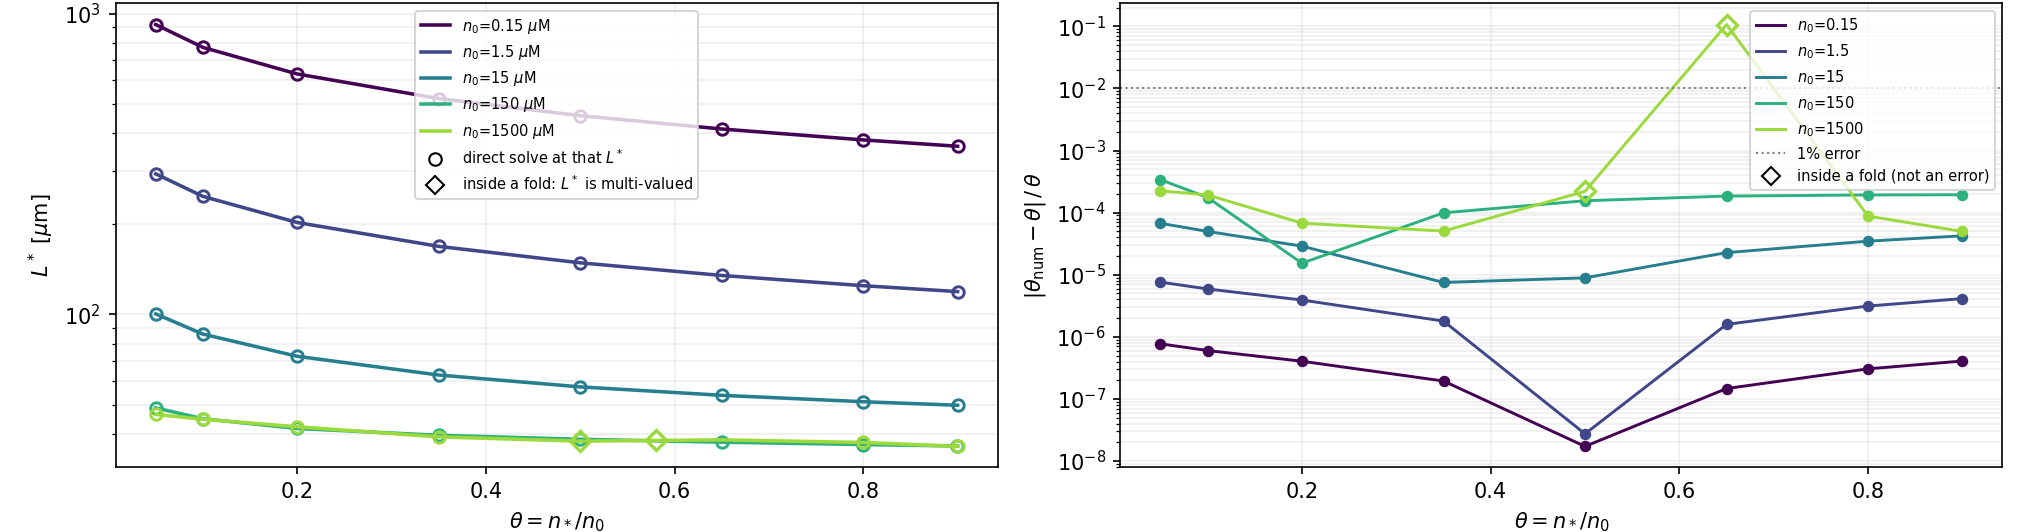
\includegraphics[width=\linewidth]{steady_lstar_general}
	\caption{(a) Numerical test of $L_*$ quadrature against direct solution at varying $n_0$, (b) the error remained well below 1\% indicating agreement. The $n_0=1500$ case contains a fold, meaning disagreement is not an error since there are multiple solutions, which will be discussed in a later section in detail \ref{sec:jamfold}.}
	\label{fig:steadylstargeneral}
\end{figure}
\FloatBarrier
	\subsection{Budget classification}
	\label{sec:budget_classification}
	Diffusion $D_{\rm col}$ is non-monotone in the dilute state and starts to "diverge" at jamming onset, i.e. becomes very large but stays finite and measurable. As cells accumulate inside the cavity, there is less space for a cell to individually move to, as such one cell moving pushes the others as well. This means that as biomass fills the cavity, cells will increasingly only be able to move as a collective rather than individually \cite{slepukhin}. In our single strain model all cells are treated as identical and in a continuum, as such individual cell movement is meaningless since there are no strains to mix. So we treat diffusion as being restricted to a collective for our steady state analysis and refrain from using self diffusion $D_{\mathrm self}$.
	\\
	Define
	\begin{equation}
		p_0:=\Psi(\rho_0),
		\qquad
		p_{\rm jam}:=\Psi(\rho_{\rm jam})
		\label{eq:p0_pjam_def}
	\end{equation}
	The terminology of a finite budget has previously been used by Giunta et al.
	to describe a fixed total amount of enzyme available to a cell \cite{enzyme}. We adopt this
	terminology for two pressure potential quantities: the pressure
	cost $B$ and the nutrient generated pressure potential budget $A$.\\
	The price to reach jamming is:
	\begin{equation}
		{
			B:=p_{\rm jam}-p_0
			=
			\Psi(\rho_{\rm jam})-\Psi(\rho_0)
			\in(0,+\infty).
		}
		\label{eq:endpoint_budget_B}
	\end{equation}
	$\rho(0)=0$ so
	$\rho_0=0$.  Normalization $\Psi(0)=0$, this reduces to
	\[
	B=\Psi(\rho_{\rm jam}).
	\]
	The integrated invariant gives
	\begin{equation}
		\Psi(\rho(x))-\Psi(\rho_0)
		=
		YD_n\bigl(n_0-n(x)\bigr).
		\label{eq:budget_invariant_general}
	\end{equation}
	the total pressure potential budget available from nutrient consumption is
	\begin{equation}
		{
			A:=YD_n n_0.
		}
		\label{eq:nutrient_budget_A}
	\end{equation}
\FloatBarrier
	\begin{figure}
	\centering
	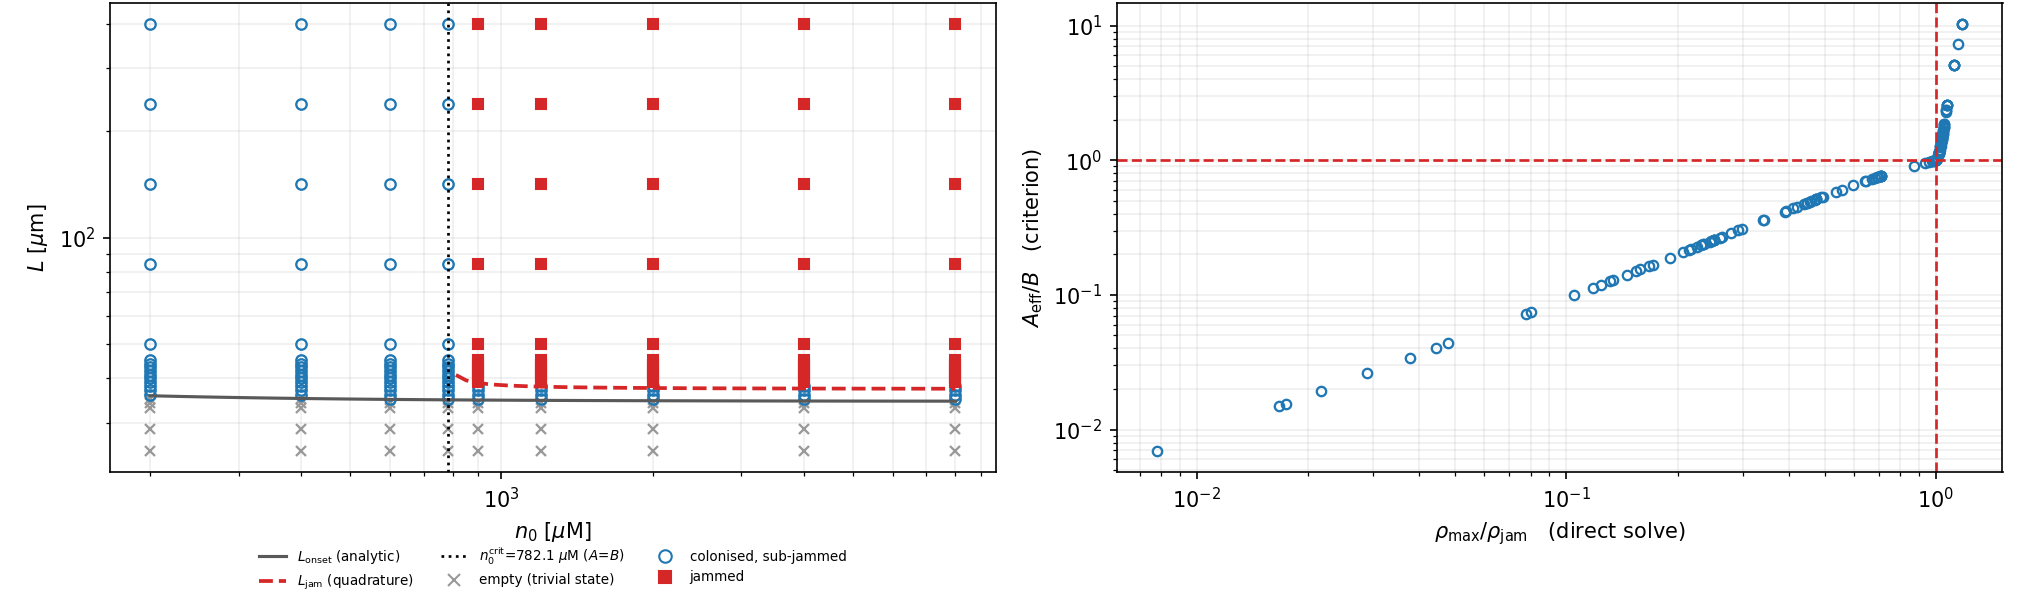
\includegraphics[width=\linewidth]{steady_budget}
	\caption{(a) Cavity phase diagram, giving population state based on a given cavity length and nutrient supply, (b) Criterion test against the numerical solver, they cross at 1 indicating perfect agreement.}
	\label{fig:steadybudget}
\end{figure}	
	As such by comparing $A$ and $B$ you can predict whether there are enough nutrients for the cavity to jam, i.e. $A<B$ dilute (insufficient budget) and $A>B$ jamming possible for a long enough cavity (exceeding budget) \ref{sec:Ljam_finite}. For $A=B$ the nutrient would be exactly depleted and as such would require an infinitely long cavity \ref{sec:n0}.
	Since we know the jamming density, $B$ can be calculated with a CAS using $D_{\mathrm col}(\rho_{\mathrm jam})=0.6864\,D_0=258.1\ \mu\mathrm{m}^2/\mathrm{h}$, so the price it costs to reach jamming is $B=\int_0^{\rho_{\mathrm jam}}\!D_{\mathrm col}(s) ds=0.7226\,D_0=271.7\ \mu\mathrm{m}^2/\mathrm{h}$. So in our system the minimum nutrient that needs to be supplied through the opening is $n_0^{\mathrm{crit}}=\frac{0.7226\,D_0}{Y D_n}=782.1 \mathrm{\mu M}$. However $A$ is the budget available to the colony, the amount actually used depends on the cavity length. \\
	\\As such we define the effective budget $A_{\mathrm eff}=YD_n(n_0-n(L))$ with $0\le A_{\mathrm eff}<A$ and thus the maximal density in the cavity is $\rho(x)\le\rho_{\mathrm max}=\Psi^{-1}(A_{\mathrm eff}(L))$. So a sufficient nutrient supply and long enough cavity is necessary for jamming. As such the cavity can only jam if $A_{\mathrm eff}>B$, a definitive criterion for jamming.
	\subsection{Monotonicity}
	\label{sec:monotonicity_new}
	Nutrient diffuses inwards from the opening and is converted into biomass, which then gets washed out through the mouth. So the further away from the opening you are the less likely you are from being washed out. However no individual cell is fixed in place and in the continuum steady state the local density is dependent on the local nutrient alone, and the balance between them is fixed by yield. Nutrient concentration must fall inwards since it is supplied through the opening being consumed everywhere and since nutrient consumption corresponds directly to increased biomass, the balance between them guarantees opposite monotone profiles. 
	From the nutrient equation
	\[
	n_{xx}=\frac{g(n)\rho}{YD_n}\ge0.
	\]
	So the slope $n_x$ is nondecreasing as $x$ increases.  Since the
	closed-end condition gives $n_x(L)=0$, all slopes to the left of
	$L$ must satisfy
	\[
	n_x(x)\le n_x(L)=0.
	\]
	Therefore $n$ is nonincreasing along the cavity towards the closed end.
	Using the invariant
	\[
	D_{\rm col}(\rho)\rho_x=-YD_n n_x.
	\]
	Because $n_x\le0$ the right hand side is nonnegative.  Since
	$D_{\rm col}(\rho)>0$, we get
	\[
	\rho_x\ge0.
	\]
	So biomass is nondecreasing along the cavity towards the closed end. As such the profile of both the biomass density and nutrient concentration is monotone in a steady state.
	\begin{figure}[ht]
		\centering
		\begin{subfigure}{0.48\textwidth}
			\centering
			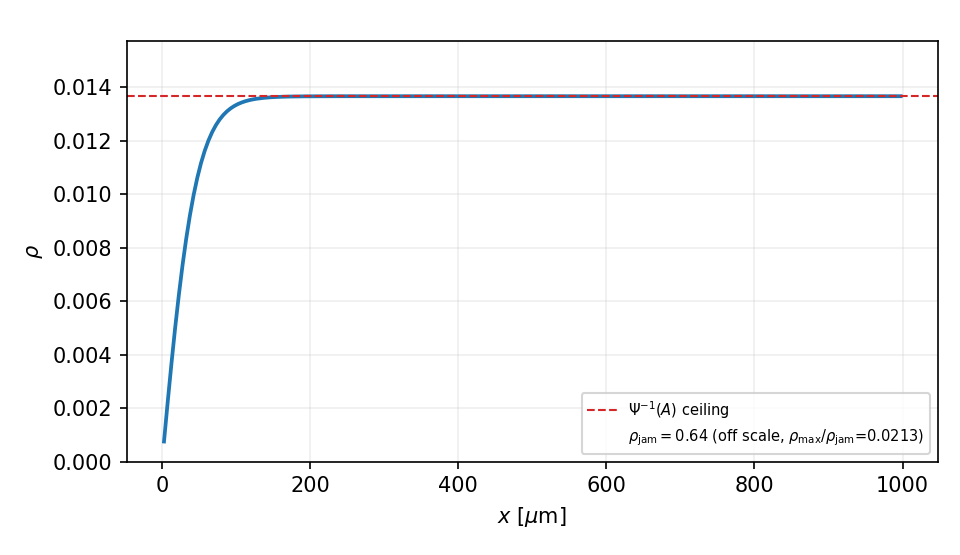
\includegraphics[width=\textwidth]{steady_density.png}
			\caption{Density profile over position}
			\label{fig:first}
		\end{subfigure}
		\hfill
		\begin{subfigure}{0.48\textwidth}
			\centering
			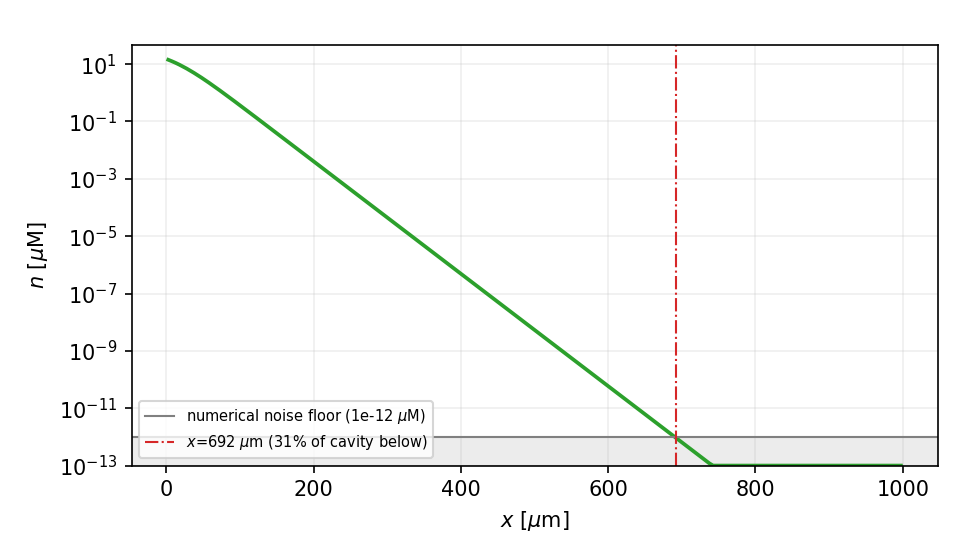
\includegraphics[width=\textwidth]{steady_nutrient.png}
			\caption{Nutrient concentration over position on a log-scale}
			\label{fig:second}
		\end{subfigure}
		\caption{Monotone spatial profiles of a dilute glutton population adhering $\rho(x)\le\rho_{\mathrm max}=\Psi^{-1}(A_{\mathrm eff}(L))$, for a 1mm long cavity. Below a nutrient concentration of approximately $10^{-12}\mu M$, the solver essentially gives numerical noise and it is not a trustworthy solution.}
		\label{fig:both}
	\end{figure}
	
	\subsection{Fully jammed approximation}
	\label{sec:jammed_bulk_new}	
	In a fully jammed cavity the density can be seen as approximately constant $\rho\approx \text{const.}$
	The biomass current is represented by an advective velocity $J_\rho=\rho_{j}v$ with $\partial_x(\rho_{j}v)=g(n)\rho_{j}$,
	so $v_x=g(n)$.
	The nutrient equation becomes $D_n n_{xx}=\frac{\rho_{j}}{Y}g(n)$.
	Under $g(n)\approx kn$ we get a Helmholtz equation of the form
	\begin{equation}
		n_{xx}-\kappa_{j}^2n=0,
		\qquad
		\kappa_{j}:=\sqrt{\frac{k\rho_{j}}{YD_n}}.
	\end{equation}
	With nutrient boundary conditions $n(0)=n_0$ and $n_x(L)=0$ we get
	\begin{equation}
		{
			n(x)=n_0
			\frac{\cosh\left(\kappa_{j}(L-x)\right)}
			{\cosh\left(\kappa_{j}L\right)}.
		}
	\end{equation}
		\begin{figure}[ht]
		\centering
		\begin{subfigure}{0.48\textwidth}
			\centering
			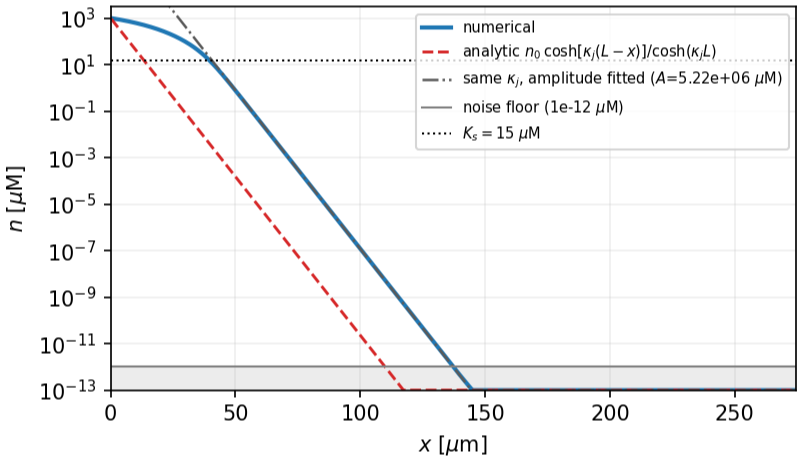
\includegraphics[width=\textwidth]{jammed_analytic_nutrient2}
			\caption{}
			\label{fig:jamn}
		\end{subfigure}
		\hfill
		\begin{subfigure}{0.48\textwidth}
			\centering
			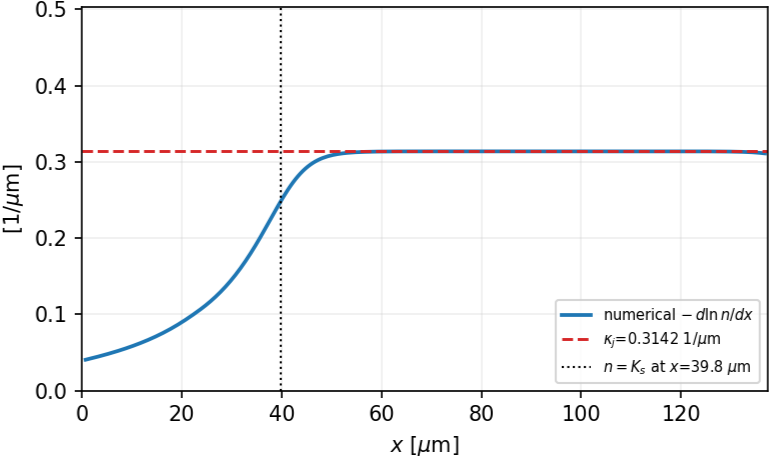
\includegraphics[width=\textwidth]{jammed_analytic_nutrient3}
			\caption{}
			\label{fig:jamk}
		\end{subfigure}
		\caption{Analytical jammed prediction vs solver solution, (a) Analytical nutrient concentration prediction against the direct numerical solution over position on a log-scale, (b) Predicted slope against numerical solution.}
		\label{fig:jam}
	\end{figure}
	The analytical prediction assumes $n(x)\ll K_s$ to linearise the Monod kinetics which overpredicts consumption and a constant density. Near the opening neither of these assumptions are fulfilled, leading to a massive regional error \ref{fig:jam}. However the shape of the decay rate is correct as it holds for the valid $n(x)<K_s$ region \ref{fig:jamk}. The $cosh$ profile also holds numerically, showing both solutions to be parallel to one another \ref{fig:jamn}, the offset is due to the large error in the opening region. So the analytical solution predicts the correct behavior and shape, however is too oversimplified to give correct values throughout. We can confidently conclude that the nutrient concentration decays exponentially in a opening fed dead end cavity.
	\subsection{The Dilute Establishment Regime}
	\label{sec:dilute_establishment}
	Now we consider the opposite regime with small biomass density, weak nutrient depletion or small nutrient supply and
	establishment from an initially dilute population. When populations are in dilute state the diffusion approximately becomes scalar $D_{\mathrm col}=D_0$, simplifying our expressions \ref{dilute}. The nutrient equations thus reduces to
\begin{equation}
	{
		n''=\frac{g(n)}{D_0}\bigl(n_0-n\bigr).
	}
\end{equation}
Our threshold length an also be reduced to
\begin{equation}
	{
		L_*
		=
		\int_{0}^{p_*}
		\frac{dp}
		{
			\sqrt{
				\frac{2}{D_0}
				\int_p^{p_*}
				s\,
				g\!\left(
				n_0-\frac{s}{YD_n}
				\right)ds
			}
	}}
\end{equation}
with
\begin{equation}
	p_*=YD_n(n_0-n_*).
\end{equation}
or if in addition the nutrient supply is also much lower than the cells saturation $n_0 \ll K_s$, we get
\begin{equation}
	{
		L_*
		=
		\int_0^{p_*}
		\frac{dp}
		{
			\sqrt{
				\frac{2k}{D_0}
				\left[
				\frac{n_0}{2}(p_*^2-p^2)
				-
				\frac{1}{3YD_n}(p_*^3-p^3)
				\right]
			}
		}.
	}
\end{equation}
	The dilute threshold formula recovers the linear establishment length in the
	zero-depletion limit \ref{sec:recovery}.
	\begin{figure}
		\centering
		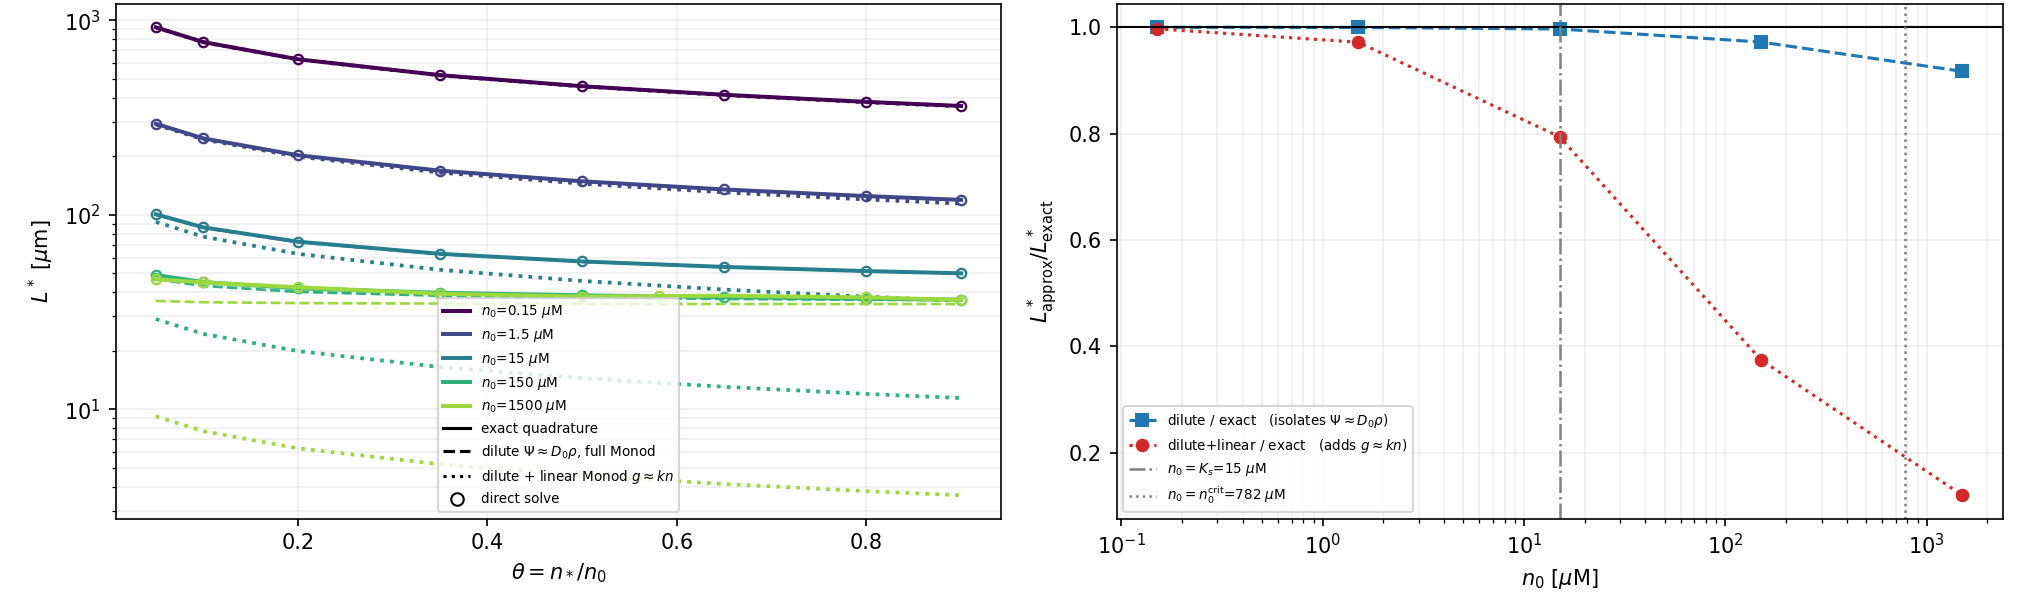
\includegraphics[width=\linewidth]{steady_lstar_dilute}
		\caption{(a) Dilute $L*$ for varying $n_0$ against direct numerical solution, general dilute approximation (stripes) and with linearized Monod law (dotted), (b) Direct difference between numerical solution and formula prediction.}
		\label{fig:steadylstardilute}
	\end{figure}
	\FloatBarrier
	\subsubsection{Spatial Profiles in the Dilute Regime}	
	The density is \begin{equation}
		{
			\rho(x)=\frac{YD_n}{D_0}\bigl(n_0-n(x)\bigr).
		}
	\end{equation}
	The integrated invariant gives \ref{dilute_profiles_corrected}	
	\begin{equation}
		n(p)=n_0-\frac{p}{YD_n}.
	\end{equation}	
and	the position at which the nutrient has value $n$ is
	\begin{equation}
		{
			x(n)
			=
			\int_n^{n_0}
			\frac{d\eta}
			{
				\sqrt{
					\frac{2}{D_0}
					\int_{n_*}^{\eta}
					g(m)(n_0-m)\,dm
				}
			}.
		}
		\label{eq:x_of_n_dilute_full}
	\end{equation}
	Under the additional low-nutrient approximation
\[
g(n)\approx kn,
\]
	\begin{equation}
	{
		x(n)
		=
		\int_n^{n_0}
		\frac{d\eta}
		{
			\sqrt{
				\frac{2k}{D_0}
				\left[
				\frac{n_0}{2}(\eta^2-n_*^2)
				-
				\frac{1}{3}(\eta^3-n_*^3)
				\right]
			}
		}.
	}
	\label{eq:x_of_n_dilute_linear}
\end{equation}

	\subsection{State transitions}
	\subsubsection{Establishment of the Colony}
	Not every cavity is able to be colonized in a steady state, if a cavity is too short a microbial community cannot find permanent shelter inside \cite{Karita}.
	\paragraph{The onset length of establishment}
	\label{sec:onset}
	The trivial state
	\begin{equation}
		\rho=0,\qquad n= n_0
		\label{eq:trivial_state}
	\end{equation}
	always solves the steady state equations for every cavity length, since when there is no biomass there is also
	no consumption. So the nutrient concentration stays $n_0$ everywhere and both equations are
	satisfied. Whether or not this uncolonised cavity is stable is what we are interested in.
	By linearising around the empty state with $\rho=\varepsilon r$ and looking at a small biomass perturbation we get
	\begin{equation}
		r_t=D_0\,r_{xx}+g(n_0)\,r,
		\qquad r(0,t)=0,
		\qquad r_x(L,t)=0
	\end{equation}
	giving the eigenvalues
	$\lambda_m=g(n_0)-D_0\left[(2m-1)\pi/2L\right]^2$ \ref{sec:trivial}. The dominant eigenvalue, i.e. slowest mode $m=1$ sets stability and is zero at
	\begin{equation}
		{\;L_{\rm onset}=\frac{\pi}{2}\sqrt{\frac{D_0}{g(n_0)}}\;}
		\label{eq:Lonset}
	\end{equation}
	giving us the minimal length a cavity needs to be in order to support a steady colony of bacteria. For a constant growth rate, this reduces identically to the establishment reported and measured by Karita \cite{Karita}.
	This transition can also be expressed using the Damköhler number which compares the diffusive time $L^2/D_0$ with the growth time $1/g(n_0)$
	\begin{equation}
		\mathrm{Da}_0:=\frac{g(n_0)L^2}{D_0},
		\qquad
		\text{establishment}\iff\mathrm{Da}_0>\mathrm{Da}_{0,c}=\frac{\pi^2}{4}.
	\end{equation}
	Growth is local while loss only happens at the opening, so the competition is
	between amplification at rate $g(n_0)$ and diffusive loss along the cavity $L$.
	If the cavity is too short cells reach the washout faster than cell growth can replace it.
	\paragraph{The transcritical onset bifurcation}
	State transitions in populations can take place in various forms, for example the jamming transition for microbial populations in cavities under nutrient rich conditions was measured to be very abrupt and characterized by a fold bifurcation \cite{Karita}. This leaves the question how the onset in characterized. For that we look at how the closed-end depletion $\delta_L:=n_0-n(L)$ grows above establishment. Near onset it follows the amplitude equation $\delta''+\kappa_0^2\delta-\beta\delta^2=0$ with $\kappa_0=\sqrt{g(n_0)/D_0}=\pi/(2L_{\rm onset})$ \cref{sec:bifurcationonset}. Since $\beta>0$ the colonised branch leaves the trivial state supercritically and grows linearly, so there is no bistability.
		\begin{equation}
		{
			\delta_L
			=
			\frac{3g_0\kappa_0}{2g_1^{\mathrm{eff}}}
			\bigl(L-L_{\rm onset}\bigr)
			+
			O\!\left((L-L_{\rm onset})^2\right).
		}
	\end{equation}
	Since densities cannot be negative physically, the transition is one sided indicating a transcritical bifurcation as opposed to a fold.
	\begin{figure}
		\centering
		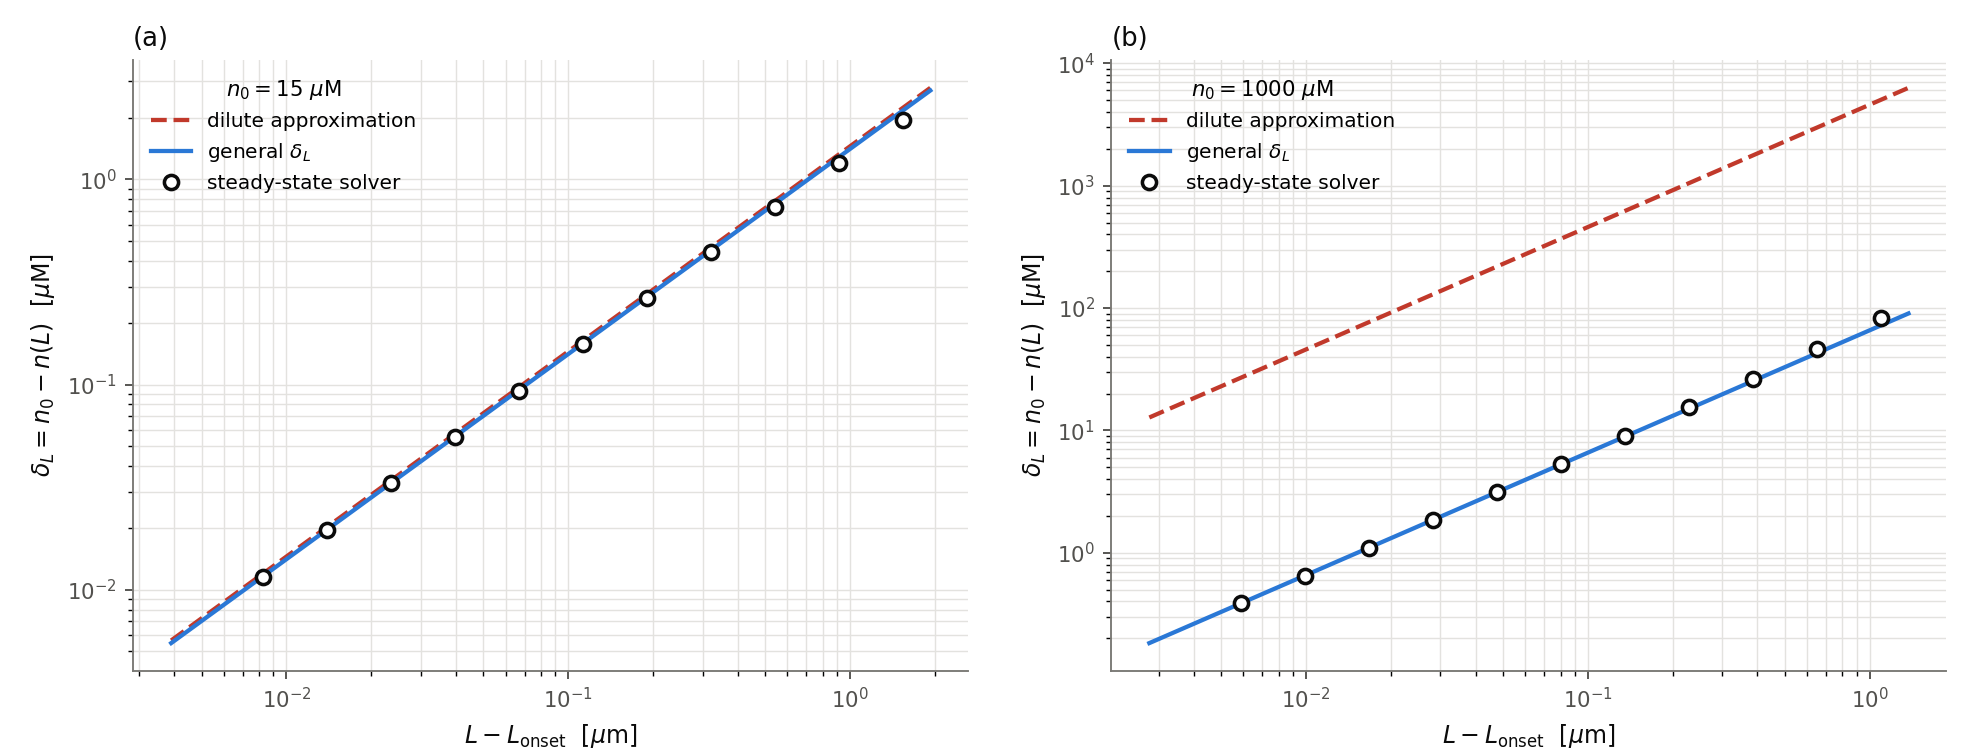
\includegraphics[width=0.7\linewidth]{onset_law_validation}
		\caption{Transcritical onset law against numerical solution.}
		\label{fig:steadyvalidation}
	\end{figure}
\newpage
	\subsubsection{Jamming transition}
	\label{sec:jamfold}

	\begin{figure}
		\centering
		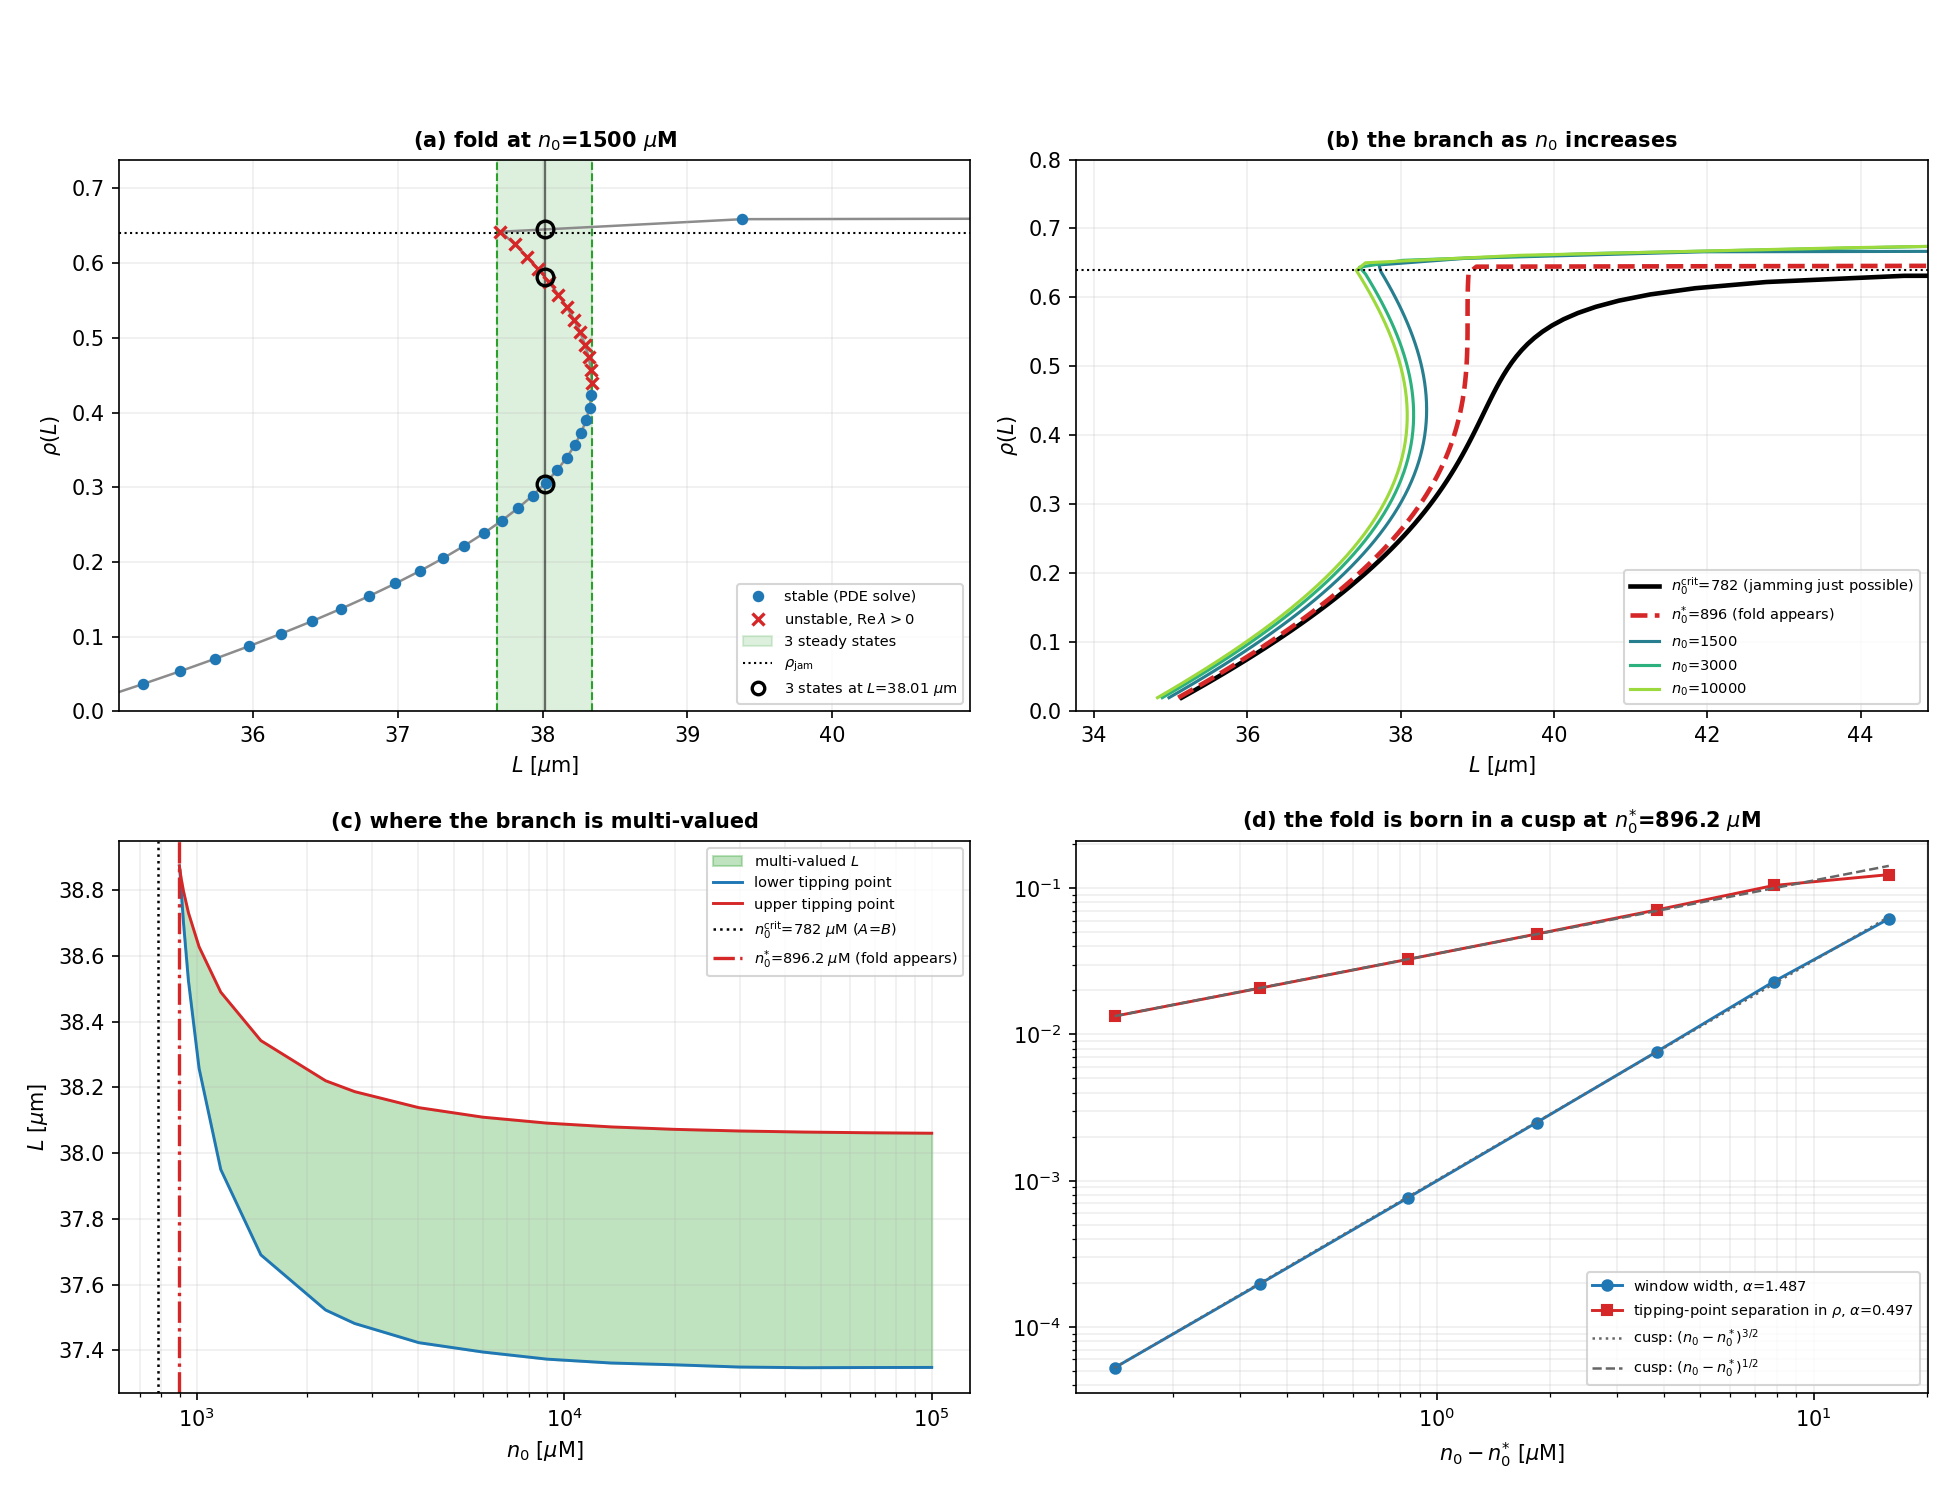
\includegraphics[width=\linewidth]{steady_fold}
		\caption{(a) density $\rho$ over cavity length $L$, showing three solutions for $L=38 \mu m$ indicating multistability producing a fold at jamming transition, two stable and one unstable state, (b) density $\rho$ over cavity length for varying $n_0$, examples with and without fold, (c) Tipping points of the fold, (d) how window width and tipping point separation scales with $n_0-n_0^{*}$.}
		\label{fig:steadyfold}
	\end{figure}
	\FloatBarrier
	In nutrient limited populations an abrupt jamming transition is not guaranteed, in fact there is a window where the jamming transition is continuous. The collective diffusion is non-monotone, with a sub-jammed peak at roughly $\rho\approx0.253$ \ref{fig:steadyclosures} and falling afterwards until it reaches jamming where the diffusivity skyrockets. Meaning that after this point, as crowding accumulates diffusive loss to the opening goes down, which again leads to increased crowding, a positive feedback loop. The system is characterized as a steady state when the diffusive loss to the opening matches new cell growth in the colony, however once bacteria reach a stable jammed state it is not easily revertible \cite{Karita}. So in nutrient rich conditions increasing cavity length leads to a discontinuous abrupt jump from a dilute to a jammed state. When $L$ is decreased back down to the same value where it was dilute earlier, the cavity remains jammed, indicating bistability. A return to a dilute population requires a lower value of $L$, see figure \ref{fig:steadyfold} panel (a), between the two tipping points three steady states coexist, of which the outer two are stable and the middle one is not.\\
\\
	This however only happens, if cells keep growing strongly in the deep end, since if cells as they approach a jammed state simultaneously also produce less biomass there is not much to be lost to the opening to keep a steady profile. The positive feedback loop has nothing to amplify, since if there is barely enough nutrients to reach jamming there is no excess that the opening fails to remove through diffusion. The nutrient budget available to cells is nearly completely spent by the time the population reaches jamming, so the monotone nutrient profile goes to zero along the cavity making the densest cells at the dead end starved. While the cells that actually still produce biomass don't sit at the dead end, making the transition to reach a steady jammed state smooth. The effective nutrient budget $A_{\mathrm eff}$ fixes the nutrients available at the dead end $n(L) = n_0 - n_0^{\mathrm{crit}}$. So a nutrient exhausted (e.g. $n_0=782.49 \mu M$, $n(L)=0$) jamming transition is gradual and completely continuous, see \ref{fig:steadyfold}, panel (b), case $n_0=782 \mu M$. We can conclude that a fold requires enough nutrients at the closed end of the cavity for there to be a phase in which the dead-end cells outproduce the interior and near opening regions.
	\\
	\\	
	Since to reach jamming we need a budget larger than $A=B$, the nutrient supply needs to be larger than $n_{0,\mathrm{crit}}=\frac{B}{YD_n}$ which for our E. coli and glucose system is $n_{0,\mathrm{crit}}=782.1\mu M$. So the $n_0=782.49$ curve in \ref{fig:steadyfold} is an extremely nutrient exhausted jammed state. Using our $L_{\mathrm onset}$ formula the colony first established between $L_{\mathrm onset}\approx 34.8\mu m$ for $n_0=782$ and at $L_{\mathrm onset}\approx 34.5\mu m$ for $n_0=10000$, the rest lies between. As panel (b) \ref{fig:steadyfold} shows, the dilute window is very short. Equally small is the continuous jamming $n_0$ window which was measured to be between	$n_{0,\mathrm{crit}}=782.1\mu M$ and $n_0^{*}=896.2\,\mu M$ with
	\begin{equation}
		{\;
			n_0^{\mathrm crit}<n_0<n_0^{*}:\ \text{continuous},
			\qquad
			n_0>n_0^{*}:\ \text{fold}
			\;}
		\label{eq:jam_two_thresholds}
	\end{equation}
	a width of $114\,\mu M$. The value $n_0^{*}$ was obtained by extrapolating the measured tipping points in \ref{fig:steadyfold} (c) (d) backwards until they cross, which is where the transition becomes continuous. Above $n_0^{*}=896.2\,\mu M$ the fold appears and multiple steady states exist for the same $L$. The tipping point separation fits the curve $(n_0-n_0^{*})^{\frac{1}{2}}$ with a measured exponent of $\alpha=0.497$ and the window width $(n_0-n_0^{*})^{\frac{3}{2}}$ with $\alpha=1.487$, \ref{fig:steadyfold} panel (d), fitting our predictions closely, \cref{sec:tipping}. For a nutrient rich cavity with supply $n_0=1500 \mu M$, this region is $L\in[37.69,38.34]\mu m$ which admits $\rho/\rho_{\mathrm jam}=0.47$, $0.91$ and $1.02$. This cavity length window scales with $\mu^{-\frac{1}{2}}$, \ref{fig:steadyfoldparams} panel (b), which aligns exactly with what our threshold length formula predicts. A numerical linear stability analysis shows that the middle one is unstable and the outer two stable \ref{fig:steadyfold}, panel (a). With increased $n_0$ above $n_0^{*}$ the fold $L$ interval saturates, panel (b), (c) and (d). 
	\begin{figure}[t]
		\centering
		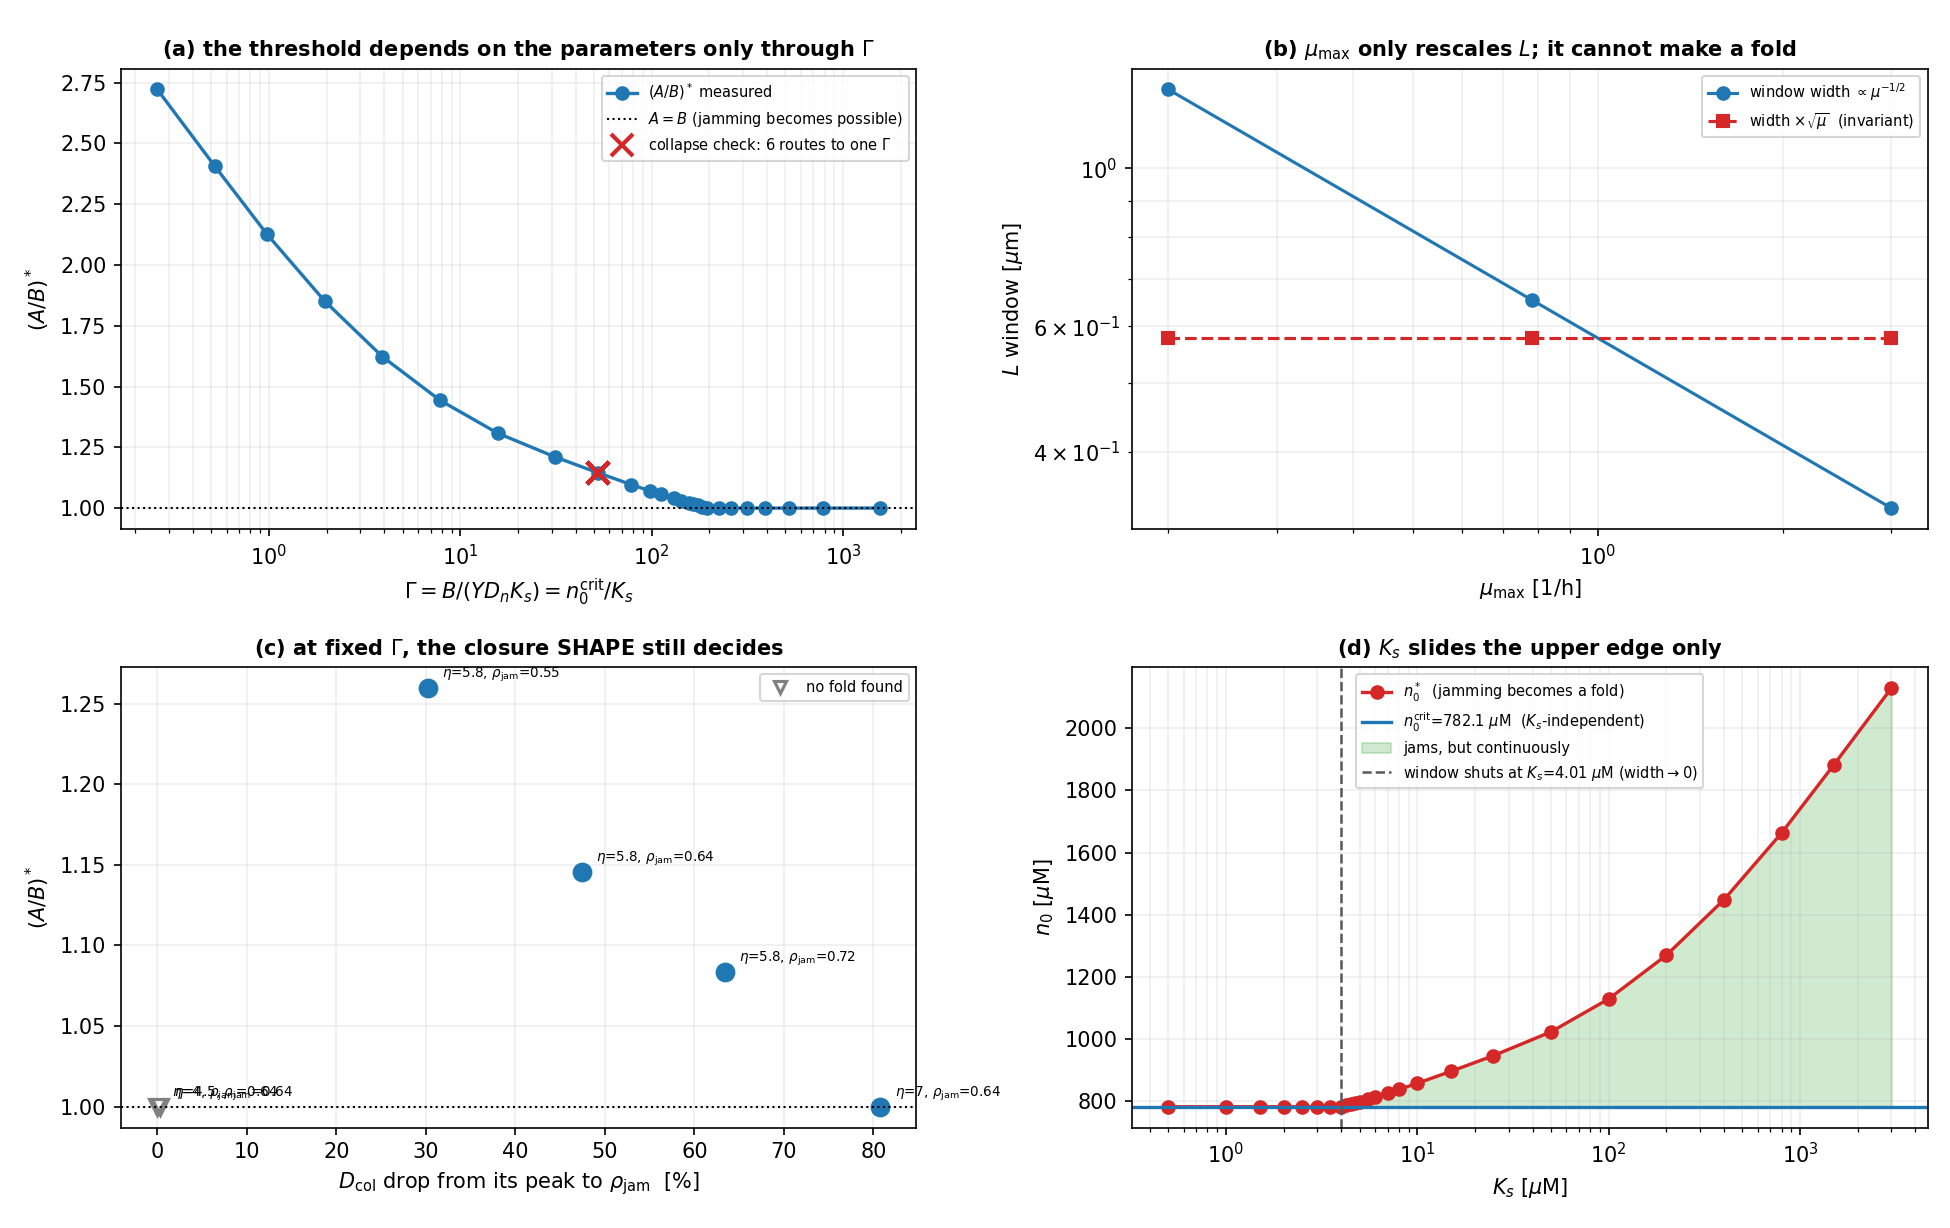
\includegraphics[width=\linewidth]{steady_fold_params}
		\caption{(a) At which effective budget $(A/B)^*$ does the jamming fold appear for a given $\Gamma=n_{0,\mathrm{crit}}/K_s$, red cross is our standard regime with $K_s=15$, (b) How does the maximal growth rate $\mu_{max}$ change the L-window inside which the fold appears, (c) Non-monotonicity of collective diffusivity is required for a fold, effective budget over $D_{\mathrm col}$, (d) Nutrient supply $n_0$ over half saturation $K_s$, increased saturation leads to larger continuous jamming $n_0$ window.}
		\label{fig:steadyfoldparams}
	\end{figure}
	Whether the continuous jamming window exists at all and how wide it is, depends on the saturation which sits inside the Monod growth law $K_s$. Values reported above were obtained using the glutton E. coli strain described in an earlier section \ref{sec:ecoli} which uses $K_s=15 \mu M$. For a small half-saturation constant $K_s$ the cells saturate on a small amount of nutrients, for $K_s\le4$ the fold appears as soon as jamming is possible, \ref{fig:steadyfoldparams} panel (d). For larger $K_s$ the continuous $n_0$ jamming windows gets increasingly wider. This constant tells us in this case how fast the left over food at the closed end is turned into biomass growth, so the important thing is whether the left over food is enough compared to $K_s$. With a small $K_s$ even a tiny nutrient concentration makes growth very fast, so when $n_0>n_0^{\mathrm crit}$ even by a small margin the deep end cells are already growing very fast and out produce the middle cells. For $K_s\le4$ and $n_{0,\mathrm{crit}}=782.1\mu M$ the growth rate is essentially constant, which reduces to Karita's regime and the fold appears instantly \cite{Karita}. Raising $K_s$ means the leftover food needs to be raised for the deep cells to have significant growth at all, so a larger relative budget $(A/B)^*$ is required for a fold, \ref{fig:steadyfoldparams} panel (a). We can define $\Gamma=n_{0,\mathrm{crit}}/K_s$ to determine whether or not the continuous jamming $n_0$ exists in the first place and how wide it is \ref{fig:steadyfoldparams}, panel (a). For $K_s=15 \mu M$ the fold appears at $n_0^{*}=896.2\,\mu M$, so $n(L)=896.2\,\mu M-782.1\mu M=114\mu M$, so between the opening and the dead end the growth only differs by $10\%$. Generally a near constant growth is required for a fold, if nutrient limitation is too strong the fold disappears.
	\newpage 
	\section{Spatial sorting between strains under nutrient competition}
		\subsection{Resource competition and spatial pattern formation}
	When two strains compete for the same limited nutrient, they do not simply sort into their own niches. In fact they can transiently or permanently dominate regions where they are heavily disfavored. We call this phenomenon "inverse sorting", as they sort inverse to their local advantage. This effect is not an artifact of initial conditions (ICs), as different ICs in the jammed regime only weakly influence dynamics and results \ref{dependence}. In the dilute regime changing seed composition can significantly change strain 1s bottleneck and the deep graveyard, they are however almost always present, so inverse sorting occurs in every case. Final composition was found to be indifferent to initial conditions.  We simulate a de novo cavity invasion, meaning a cavity initially devoid of cells gets invaded through the opening. We implements this by placing a biomass seed as a distribution centered around $x=25 \mathrm{\mu m}$ as a $50:50$ mixture between the two strains, i.e. $f=0.5$. Initially the cavity is filled with nutrients, making $n(x,t=0)=n_0$ along the entire cavity. 
	\subsubsection{Dilute populations}
	\begin{figure}
		\centering
		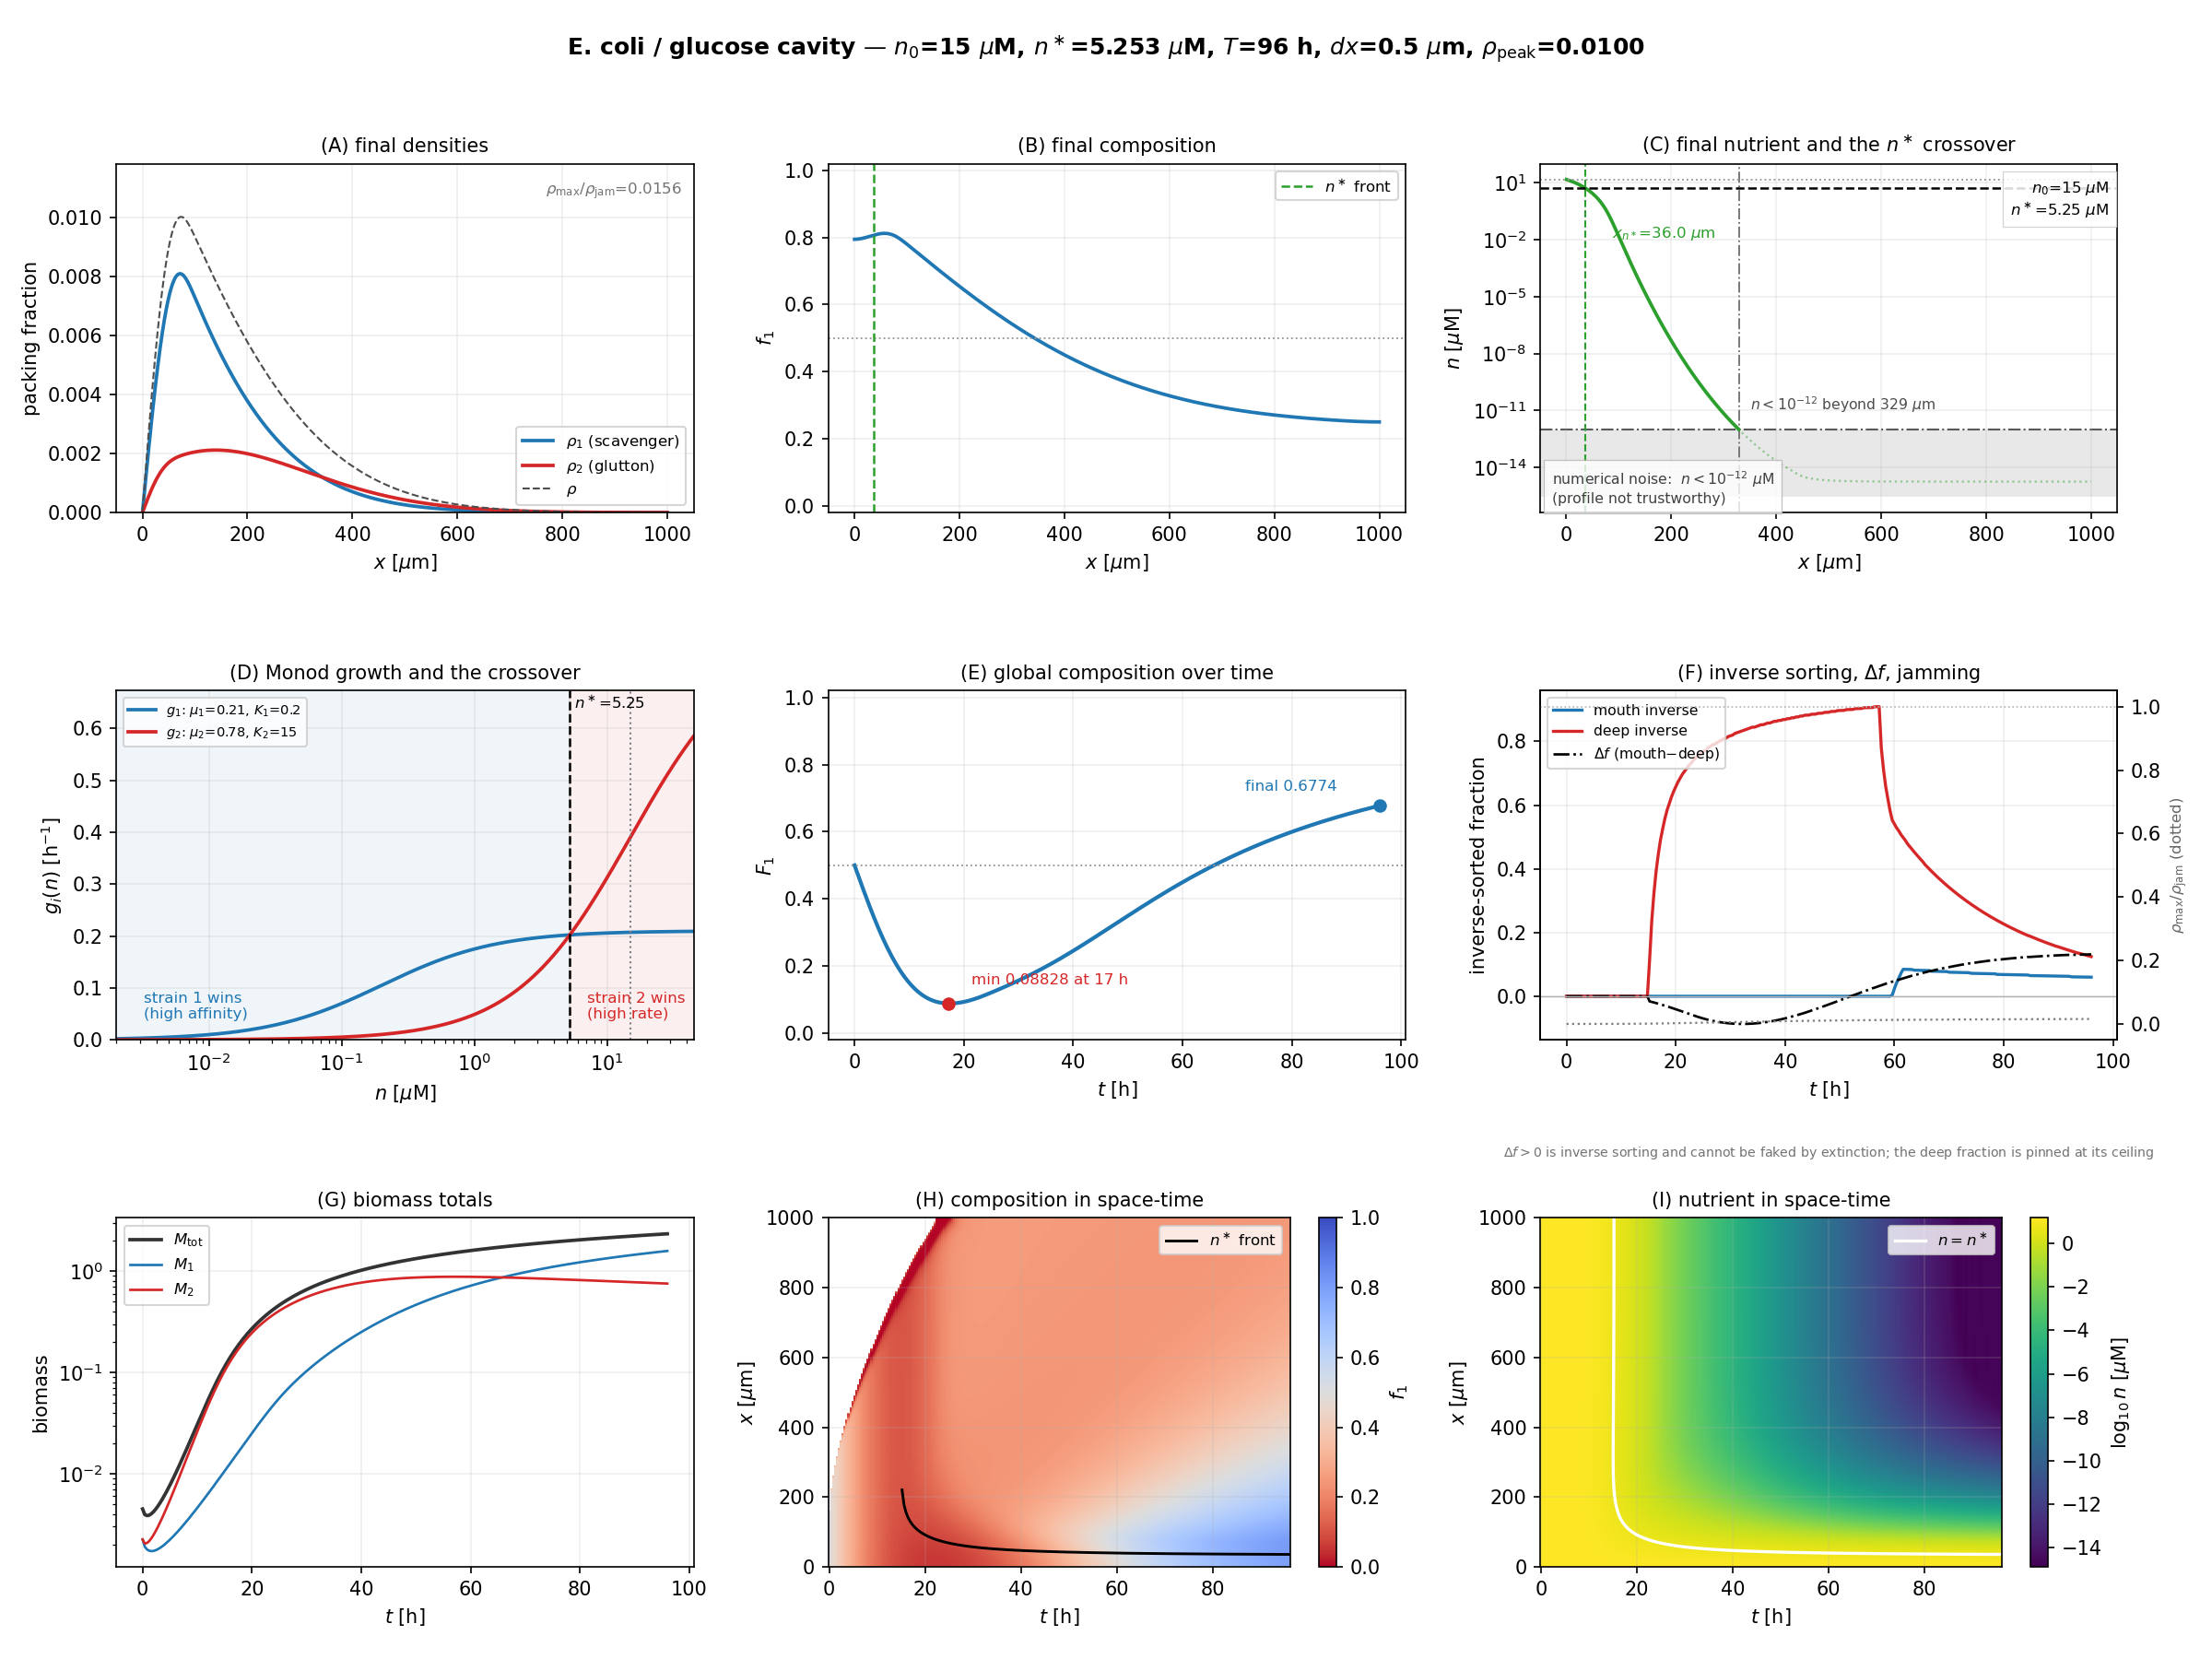
\includegraphics[width=\linewidth]{run_noise_dilute}
		\caption{(A) Strain densities over position along the cavity at final time $T=96h$, cavity is entirely dilute, (B) Strain 1 fraction over position at final time, (C) Final nutrient profile on a log-scale, for a concentration under $10^{-12} \mathrm{\mu M}$ it can no longer confidently be solved, as such considered numerical noise, (D) Strain Monod growth functions, crossover at $n^*=5.25 \mathrm{\mu M}$, (E) Global strain function over time, bottleneck near $T=17h$ strain 1 hits its low point and recovers, (F) Inverse sorted biomass fraction over time, divided into deep strain 2 graveyard "deep inverse" and opening strain 1 domination "mouth inverse", (G) Total biomass over time, integrated density, (H) space-time heat map of the composition, (I) space-time heat map of the nutrient concentration}
		\label{fig:rundilute}
	\end{figure}
	During first colonization the glutton is heavily favored everywhere, since the cells enter through the opening the only one growing is the high nutrient specialist. It quickly gets advected inwards and colonizes the entire cavity \ref{fig:rundilute}\ref{sec:kernel}, by $T=17h$ it almost completely excluded the high affinity strain. Including the deep interior where it seeks refuge, being essentially stranded there due to the absence of flux at the deep end. As the nutrient gets eaten up, this area favors the scavenger, however the glutton still dominates there since earlier in time it had such a big advantage and got advected into this area. After it hits near extinction the high affinity specialist is finally able to establish itself now that a lot of the nutrients in the cavity were eaten up. The interior nutrients were eaten by the glutton earlier and only resupplied through the opening, which leads to the crossover $n^*$ appear and quickly move to the opening. This makes almost the entire cavity favor strain 1, however absolute growth is only large enough close to the opening and such the vast majority of biomass contribution originates from a small band near the opening \ref{sec:prod}, which now sits around $n^*$. As it the crossover gets closer to the opening, newly produced glutton strains quickly get washed out before they can establish themselves. While the high affinity strain now grows quickly just behind $n^*$, part of it washed out through the opening, making it even dominate the opening region, the other part advected inwards taking over the cavity. With time it replaced the glutton graveyard stranded in the interior and wins the race by dominating the entire cavity \ref{fig:rundil1000}. This coincides with Tilmans $R^*$ limit, which predicted the strain with lower $R^*$ to exclude the other, so $F=1$ (\cref{sec:dillimit}, \cref{sec:rstar}) \cite{rstar}.
	\subsubsection{Nutrient rich and jammed populations}
	When a population is subject to a large nutrient concentration, they grow very fast and are quick to enter a jammed state. Even though the general dynamics of the near extinction and following recovery of the high affinity, an entirely jammed cavity does not converge to the $R^*$ rules expected result of its global domination and exclusion of the glutton. Around $T=2000h$ net biomass no longer grows, its density ceiling was already reached. As such the composition is frozen in time, the glutton still completely dominates the deep end where it is locally disfavored and equally the high affinity strain dominated the opening region where the glutton has the local advantage. Self diffusion has hit its low, very small but still not zero which causes strains to mix very slowly amongst themselves, blurring the sharp segregation slightly over long period of time. However unlike in the dilute state, inverse sorting is not a transient, it the inverse sorted biomass gets frozen in time and becomes permanent within any starved cells lifespan.	
	\begin{figure}
		\centering
		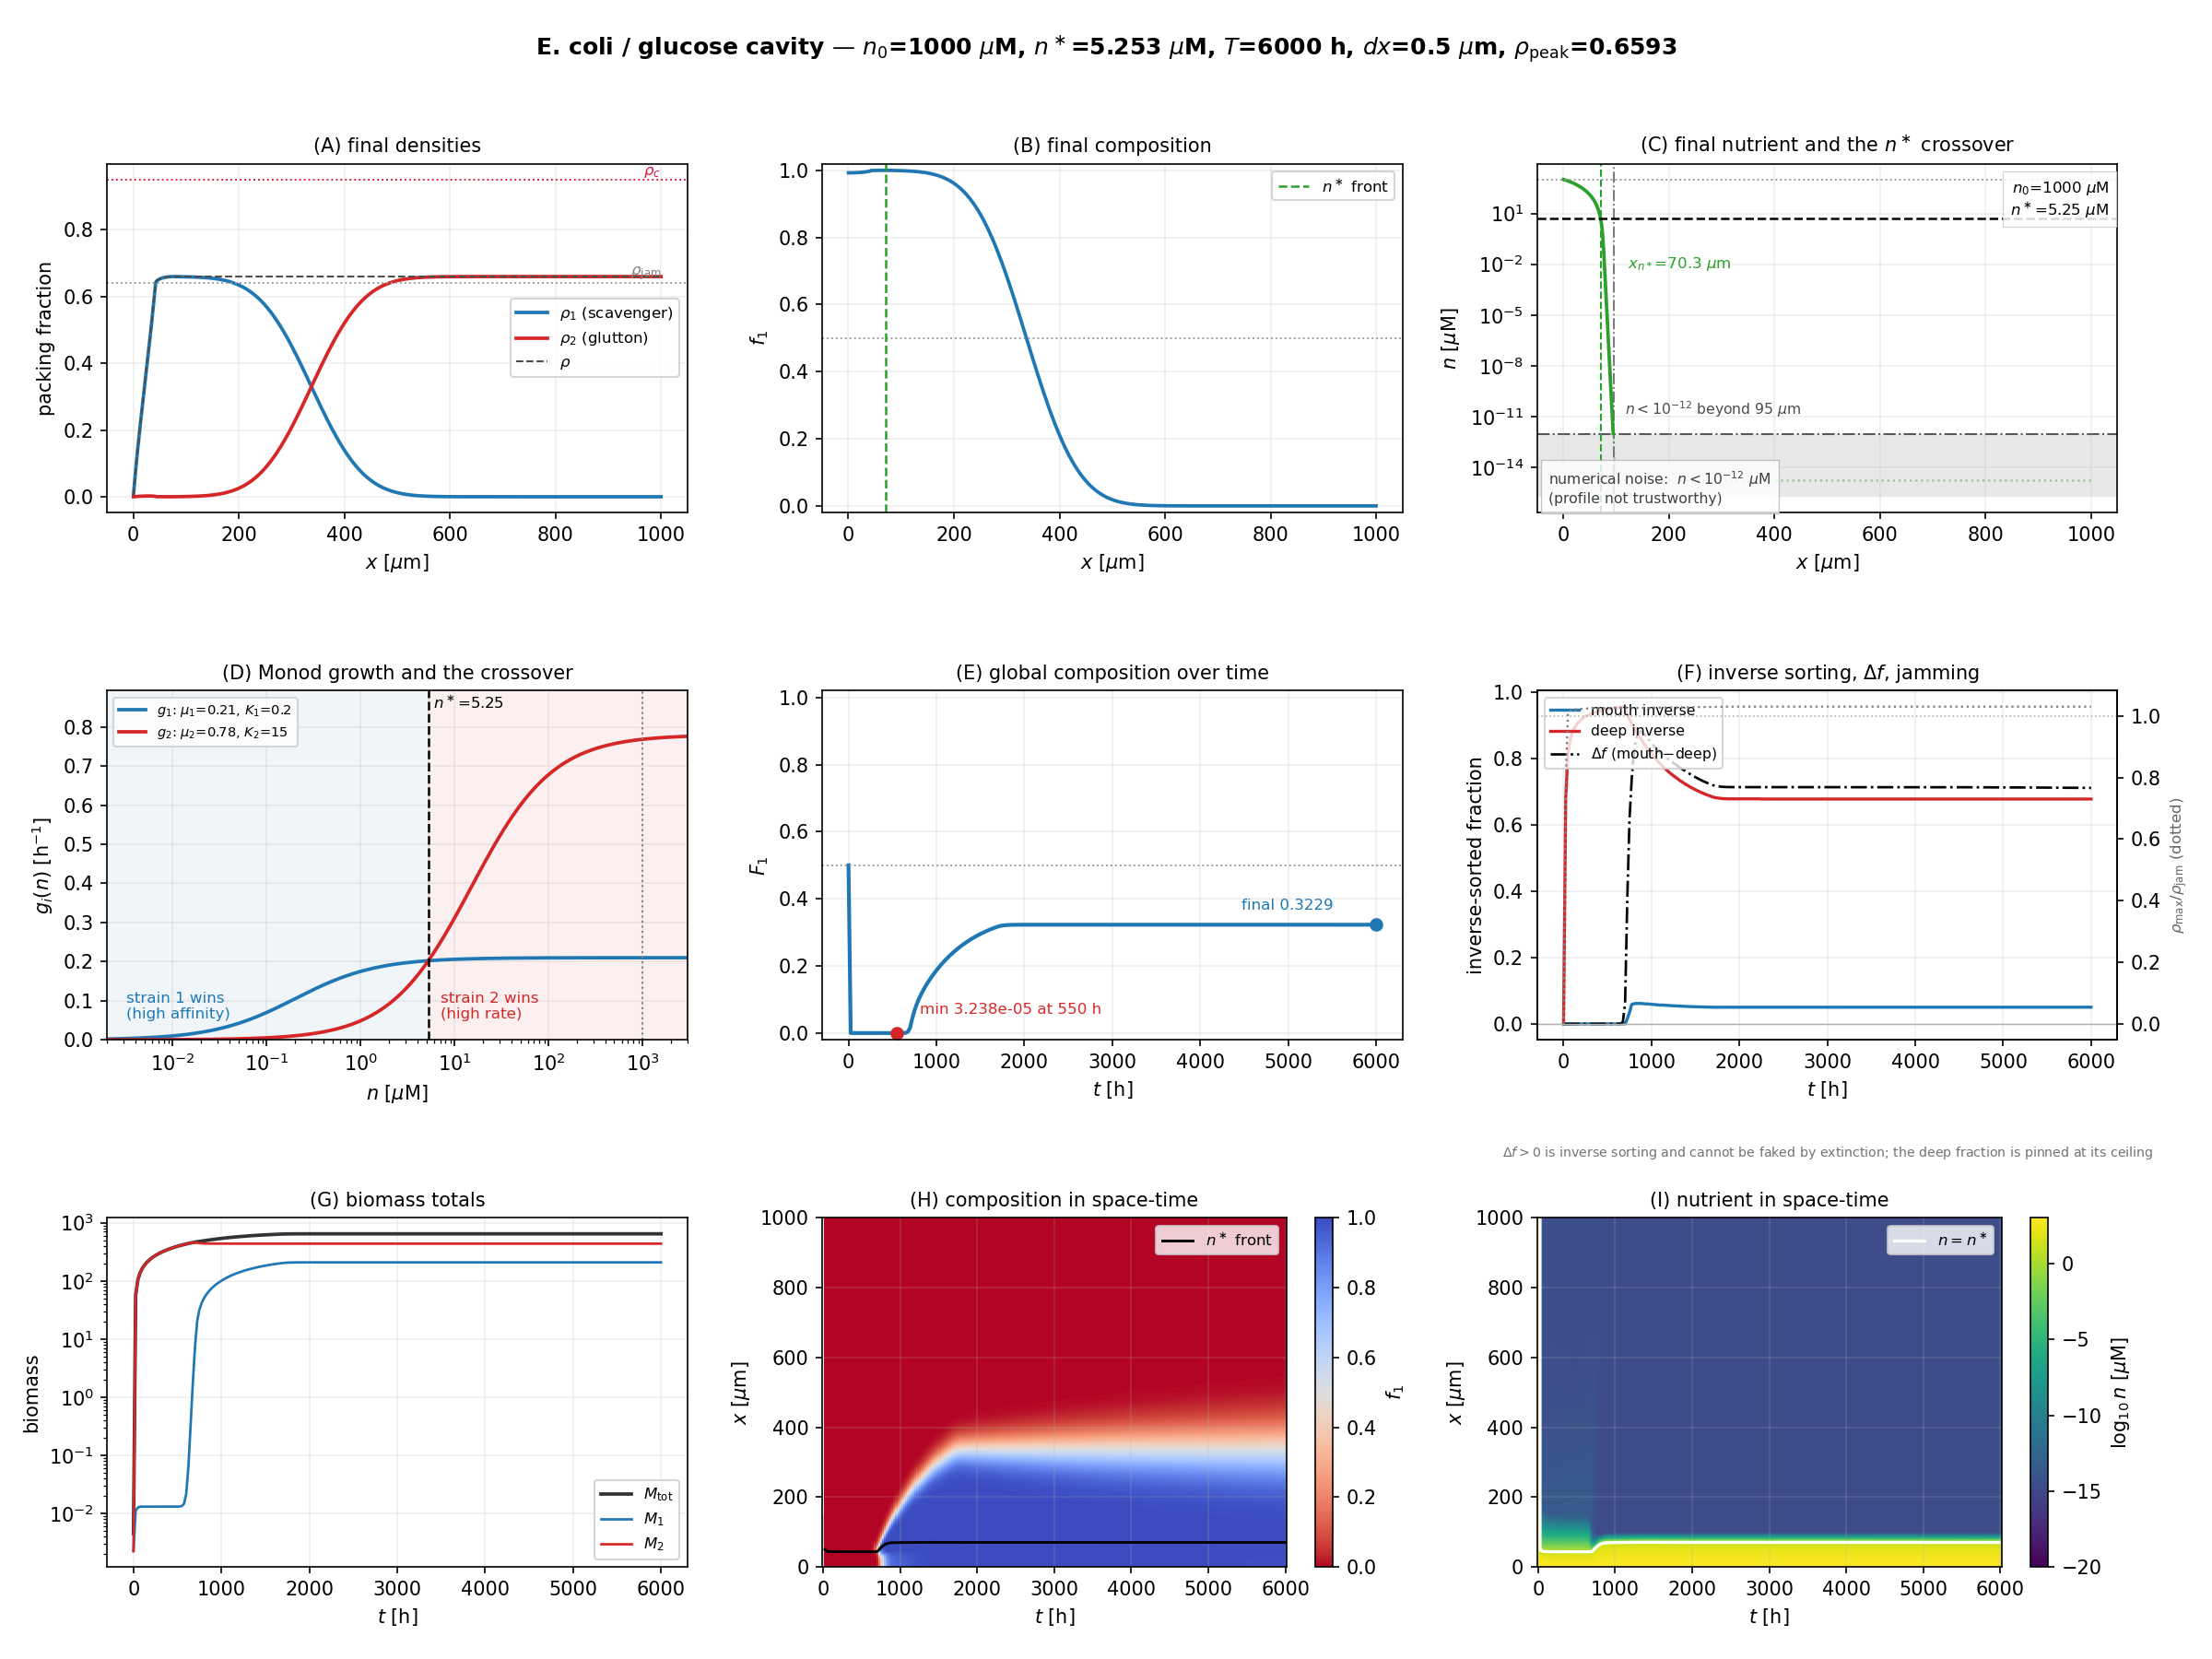
\includegraphics[width=\linewidth]{run}
		\caption{(A) Strain densities over position along the cavity at final time $T=6000h$, cavity is entirely jammed, (B) Strain 1 fraction over position at final time, (C) Final nutrient profile on a log-scale, for a concentration under $10^{-12} \mathrm{\mu M}$ it can no longer confidently be solved, as such considered numerical noise, (D) Strain Monod growth functions, crossover at $n^*=5.25 \mathrm{\mu M}$, (E) Global strain function over time, bottleneck near $T=550h$ strain 1 becomes near extinct and recovers, (F) Inverse sorted biomass fraction over time, divided into deep strain 2 graveyard "deep inverse" and opening strain 1 domination "mouth inverse", (G) Total biomass over time, integrated density, (H) space-time heat map of the composition, (I) space-time heat map of the nutrient concentration}
		\label{fig:runjam}
	\end{figure}
\subsubsection{Spatial heterogeneity}
Not every population is equally strongly sorted, in a jammed colony inside a very long 1mm cavity the two strains are much more segregated from another than a short dilute cavity. Spatial heterogeneity \ref{sec:heterozygosity} was measured to monotonically increase with cavity length and nutrient supply \ref{fig:fstpeakvsl}. The glutton and high affinity strain in a dilute $100 \mathrm{\mu m}$ cavity can be described as well-mixed, due to there being no difference in composition over position at a fixed point in time. The general mechanism of high nutrient glutton expansion phase into the deep and late recovery of the high affinity specialist is identical across cavity lengths, however in the short cavity they take place sequentially separated by time. One should note that nutrient concentration and density are not equally distributed, only the strain configuration is approximately well mixed in position at a fixed point in time.
\newpage
	\subsection{Theoretical description of the problem}	
	The evolution of composition can be expressed by the fraction equation \ref{ancestrytheory}
	\begin{equation}
		{
			\pd_t f+u\pd_xf
			=\frac1\rho\pd_x(\Dself\rho\pd_xf)+f(1-f)s(n).
		}
		\label{eq:f-equation}
	\end{equation}	
	The sign of the variable \(h=2f-1\) gives local dominance
	\begin{equation}
		{
			\pd_t h=\Lop_t h+\frac12(1-h^2)s(n),
		}
		\label{eq:h-equation}
	\end{equation}
	where the neutral transport operator is
	\begin{equation}
		{
			\Lop_t\phi=-u(x,t)\pd_x\phi+\frac1{\rho(x,t)}
			\pd_x\left[\Dself(\rho(x,t))\rho(x,t)\pd_x\phi\right].
		}
		\label{eq:Lop}
	\end{equation}
	\(\Lop_t\) describes the transport of a passive strain label when removing the selective growth difference. Selection only happens through the source term \(\frac12(1-h^2)s\).
	\begin{equation}
		{
			h(x,T)
			=
			\int_0^L K(y,0\mid x,T)h_0(y)\,dy
			+
			\frac12
			\int_0^T\int_0^L
			K(y,t\mid x,T)
			\bigl(1-h(y,t)^2\bigr)s(n(y,t))\,dy\,dt .
		}
		\label{eq:duhamel-kernel2}
	\end{equation}
	This is a deterministic Greens function representation of the continuum ancestry dynamics. The first
	term is the neutral transport of the initial dominance field. The second term
	is the neutral transport from every earlier space time point \((y,t)\) to the
	final point \((x,T)\) of the realized local selection source. $K$ weights the contribution of an earlier point in time to a final point in time as a distribution, it is normalized and non-negative. It is analogous to the backwards density $G(\xi,\tau\mid x,t)$ by Nelson \& Hallatschek \cite{gene} \cite{lifeexp}. The Duhamel solution is implicit in its nature.
	\begin{figure}[htbp]
		\centering
	\begin{subfigure}{0.45\textwidth}
		\centering
		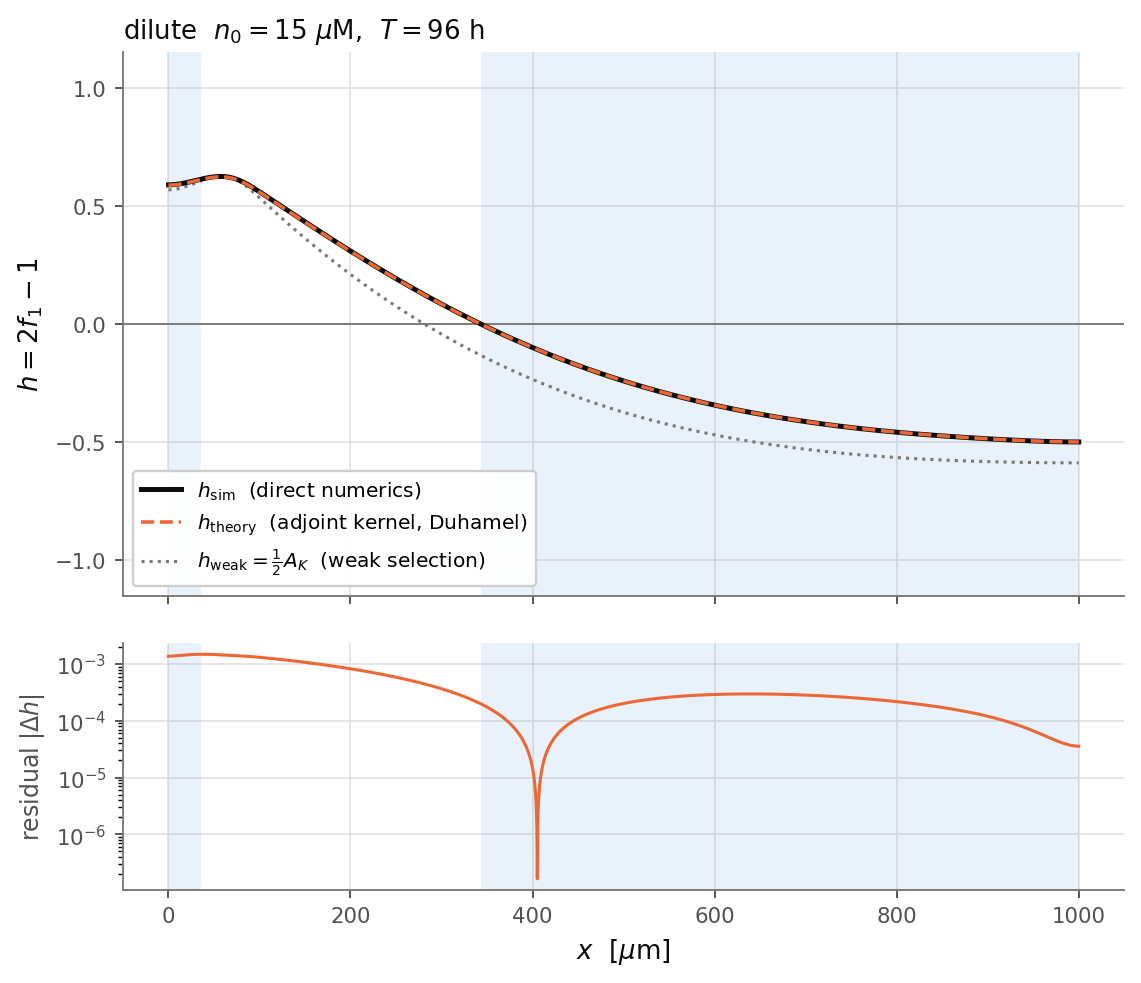
\includegraphics[width=\textwidth]{h_theory_vs_numericdil}
		\caption{Dilute, $T=96h, n_0=15 \mathrm{\mu M}$}
		\label{fig:hdil}
	\end{subfigure}
	\hfill
	\begin{subfigure}{0.45\textwidth}
		\centering
		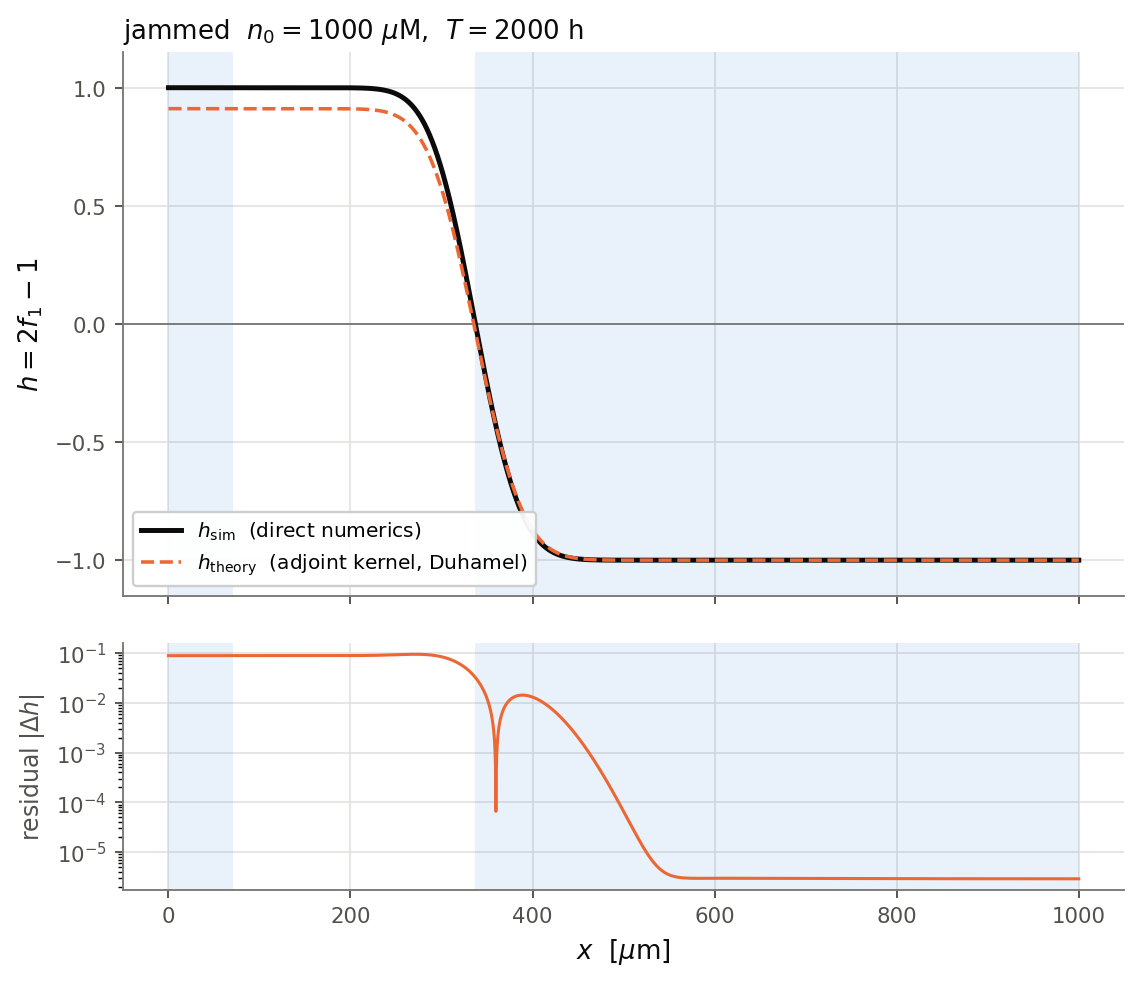
\includegraphics[width=\textwidth]{h_theory_vs_numeric}
		\caption{Jammed, $T=2000h, n_0=1000 \mathrm{\mu M}$}
		\label{fig:hjam}
	\end{subfigure}
	\caption{Analytical solution of the dominance variable at a fixed point in time against direct numerical solution in the dilute and jammed regime. The inverse sorted sections are shaded blue.}
\end{figure}
	\label{fig:h}
	\subsubsection{Weak selection approximation}
	
	If \(|h|\ll1\) then
	\begin{equation}
		1-h^2=1+O(h^2),
	\end{equation}
	and the duhamel solution reduces to
	\begin{equation}
		h(x,T)\approx
		\int_0^L K(y,0\mid x,T)h_0(y)\dd y
		+\frac12\int_0^T\int_0^L K(y,t\mid x,T)
		s(n(y,t))\dd y\dd t.
		\label{eq:weak-continuum}
	\end{equation}
	For a uniform 50:50 initial condition \(h_0=0\)
	\begin{equation}
		h(x,T)\approx\frac12 A_K(x,T),
		\label{eq:h-ak}
	\end{equation}
	where the kernel weighted history is
	\begin{equation}
		A_K(x,T)=\int_0^T\int_0^L K(y,t\mid x,T)s(n(y,t))\dd y\dd t.
		\label{eq:AK}
	\end{equation}
	\subsubsection{Inverse sorting criterion}
	Let
	\begin{equation}
		s_T(x)=s(n(x,T)).
	\end{equation}
	The local environment favors strain 1 when \(s_T(x)>0\) and favors strain 2 when \(s_T(x)<0\). The local dominant strain is given by the sign of \(h(x,T)\). So inverse sorting at \(x\) is defined by
	\begin{equation}
		{
			h(x,T)s_T(x)<0.
		}
		\label{eq:inverse-def}
	\end{equation}
	
	\subsubsection{Exposure decomposition}
	Assume that \(h_0=0\). Define
	\begin{equation}
		\sigma_T(x)=\sgn s_T(x).
	\end{equation}
	Because \(1-h^2\geq0\) and \(K\geq0\), the source contribution can be split into a part that reinforces the final local selection sign and a part that opposes it.  Define
	\begin{align}
		A_+(x,T)&=\int_{\sigma_T(x)s(n(y,t))>0}
		K(y,t\mid x,T)[1-h(y,t)^2]|s(n(y,t))|\dd y\dd t,
		\label{eq:Aplus}\\
		A_-(x,T)&=\int_{\sigma_T(x)s(n(y,t))<0}
		K(y,t\mid x,T)[1-h(y,t)^2]|s(n(y,t))|\dd y\dd t.
		\label{eq:Aminus}
	\end{align}
	\eqref{eq:duhamel-kernel2} gives
	\begin{align}
		\sigma_T(x)h(x,T)
		&=\frac12\left[A_+(x,T)-A_-(x,T)\right].
		\label{eq:sigmah-exposure2}
	\end{align}
	\begin{theorem}[inverse sorting criterion for neutral initial composition]
		Assume \(h_0=0\), \(K\geq0\) and the final selection is nonzero at \(x\). Then inverse sorting occurs at \(x\) if and only if
		\begin{equation}
			{A_-(x,T)>A_+(x,T).}
			\label{eq:exposure-criterion2}
		\end{equation}
	\end{theorem}	
	\begin{proof}
		By definition inverse sorting means \(h(x,T)s_T(x)<0\). Since \(s_T(x)\neq0\) this is equivalent to \(\sigma_T(x)h(x,T)<0\). Using \cref{eq:sigmah-exposure2} we get
		\begin{equation}
			\frac12[A_+(x,T)-A_-(x,T)]<0,
		\end{equation}
		or \(A_-(x,T)>A_+(x,T)\).
	\end{proof}
	If \(h_0\neq0\) define the inherited initial contribution
	\begin{equation}
		B_0(x,T)=\sigma_T(x)\int_0^L K(y,0\mid x,T)h_0(y)\dd y.
	\end{equation}
	Then
	\begin{equation}
		\sigma_T(x)h(x,T)=B_0(x,T)+\frac12[A_+(x,T)-A_-(x,T)].
	\end{equation}
	the criterion becomes
	\begin{equation}
		{
			A_-(x,T)>A_+(x,T)+2B_0(x,T).
		}
		\label{eq:exposure-with-initial}
	\end{equation}
	This is why in patchy initial conditions inverse sorting can be caused or suppressed by the transported initial label field.
	\begin{figure}[htbp]
	\centering
	\begin{subfigure}{0.45\textwidth}
		\centering
		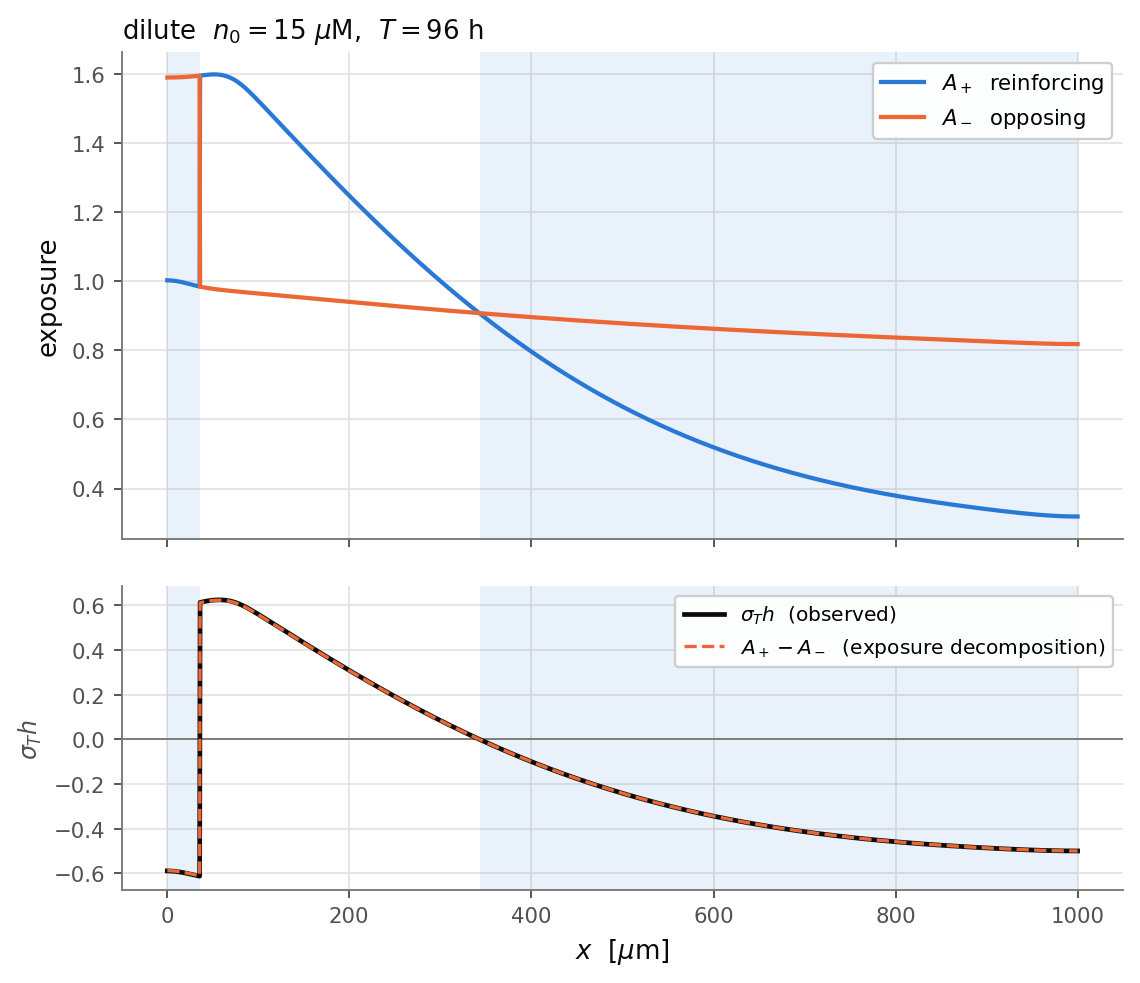
\includegraphics[width=\textwidth]{criteriondilute}
		\caption{Dilute, $T=96h, n_0=15 \mathrm{\mu M}$}
		\label{fig:adil}
	\end{subfigure}
	\hfill
	\begin{subfigure}{0.45\textwidth}
		\centering
		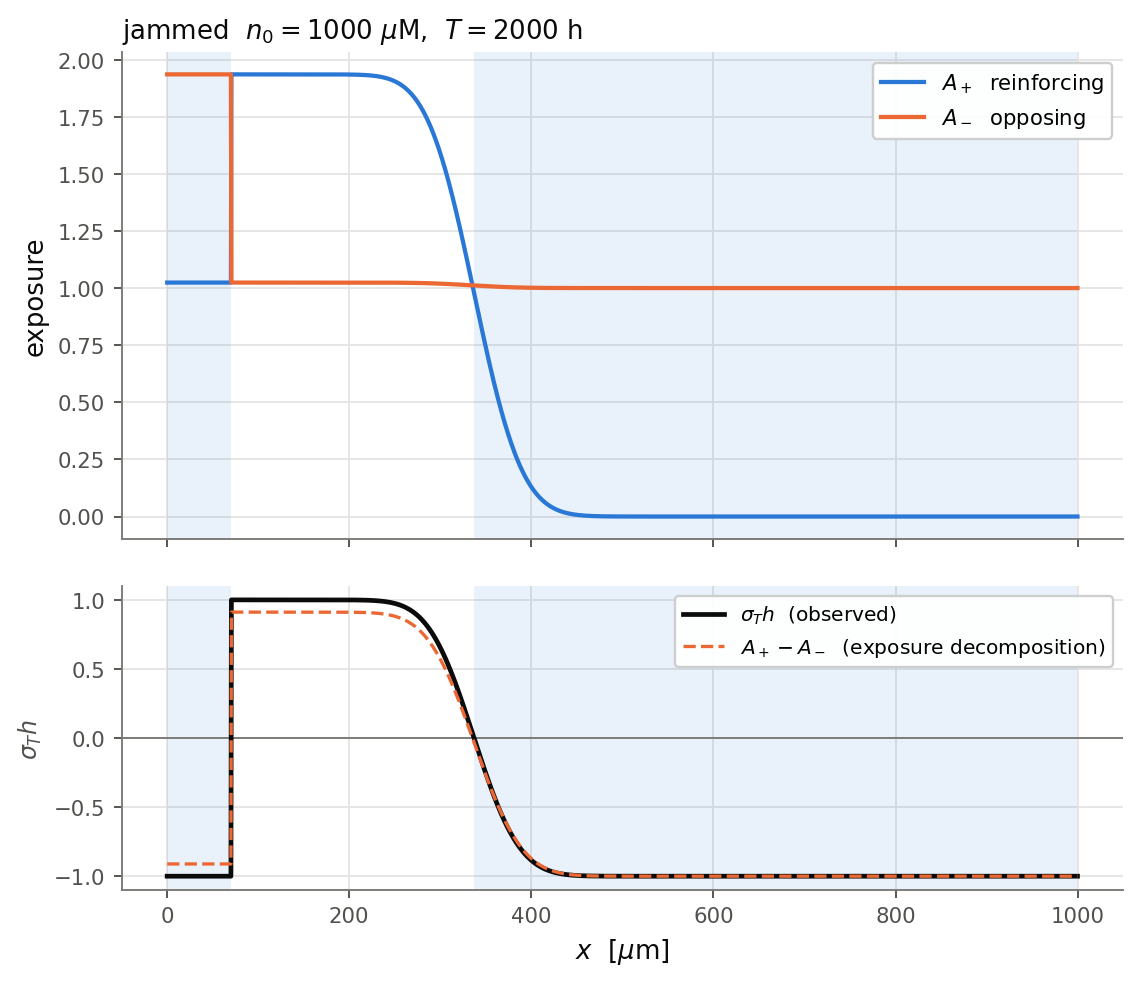
\includegraphics[width=\textwidth]{criterioninversejam}
		\caption{Jammed, $T=2000h, n_0=1000 \mathrm{\mu M}$}
		\label{fig:ajam}
	\end{subfigure}
	\caption{Exposure decomposition to categorize inverse sorting.}
\end{figure}
\label{fig:a}
\subsection{Numerical physiology}
\paragraph{Varying seed}
The main simulations all considered an invasion colonization though the opening, equally seeded strains and a very low initial biomass. A larger seed colonizing a cavity results in accelerated dynamics, the result however remains the same in a dilute setting with the Tilman $R^*$ $F_1=1$ limit. With a large enough seed density of $\rho_{\mathrm{seed}}=0.01$ the initial nutrient expansion phase that usually results in the inverse sorted glutton graveyard in the deep end can be skipped entirely and the high affinity strain takes over right from the start monotonically \ref{fig:dilutedensity}. In the jammed case it shifts to being slightly in favor of the high affinity strain, however behavior is identical \ref{fig:jamdensity}. Rigging the game from the start by seeding more of one strain over the other, i.e. varied $f_1$ of the seed, had little effect on the general dynamic process apart from favoring the advantaged strain. Even with a $f_1=0.9$ seed, as long as it is small the nutrient expansion phase of the glutton is inevitable \ref{fig:seedf1}. Changing the colonization type by comparing the invasion to an uniformly seeded biomass along the entire cavity and one starting from the deep end had no strong effect in the jammed cavity \ref{fig:seedmode}. In a dilute cavity a deep or uniform seed does eridicate the initial glutton expansion. As seen in panel (C) with deeply seeded biomass or a uniform distribution, initially during the early phase there is more normally sorted biomass in the dilute case. The victory of the high affinity strain is undisputed, all of them have the same $F_1=1$ limit. In the jammed case there is almost no difference, the only one being by placing some of the high affinity strain inside the cavity by a uniform seed gives it a slight advantage.
\paragraph{Initial nutrients}
Changing the initial conditions of nutrients, i.e. if the cavity is filled with food from the start, empty or linearly distributed across, was found to have no measurable effect in both the dilute and jammed regime \ref{fig:nutrientic}.
\subsubsection{Biomass production}
\label{sec:prod}
In both the dilute and jammed regime biomass is almost exclusively being produced near the opening, due to the absolute growth rate being too low in the interior and the deep end \ref{fig:g}. Biomass production is defined as $P=\rho_{i} g_{i} q$. So which strain is being mass produced is set almost entirely by the position of the $n^*$ front at the opening. So early on in the dilute regime the crossover is still in the interior, such that the glutton is a strong favorite in selection and as such gets mass produced while the high affinity strain gets left behind. As time goes on the front moves towards the opening, resulting in a recovery and eventual global domination of the high affinity strain which originates from just behind the crossover near the opening later in time. After 500 hours of dilute colonization, $90\%$ of produced biomass was made in the interval between $0\mathrm{\mu m}\le x\le 75 \mathrm{\mu m}$ \ref{fig:gdil}, panel (D), in a jammed cavity it is even more narrow with $0\mathrm{\mu m}\le x\le 63 \mathrm{\mu m}$ after 2000 hours \ref{fig:gjam}, panel (D). This has previously been observed in oxygen limited biofilm protein synthesis, where production was observed in a narrow band between oxygen supply and biofilm bulk \cite{produ}.
\begin{figure}[htbp]
	\centering
	\begin{subfigure}{\textwidth}
		\centering
		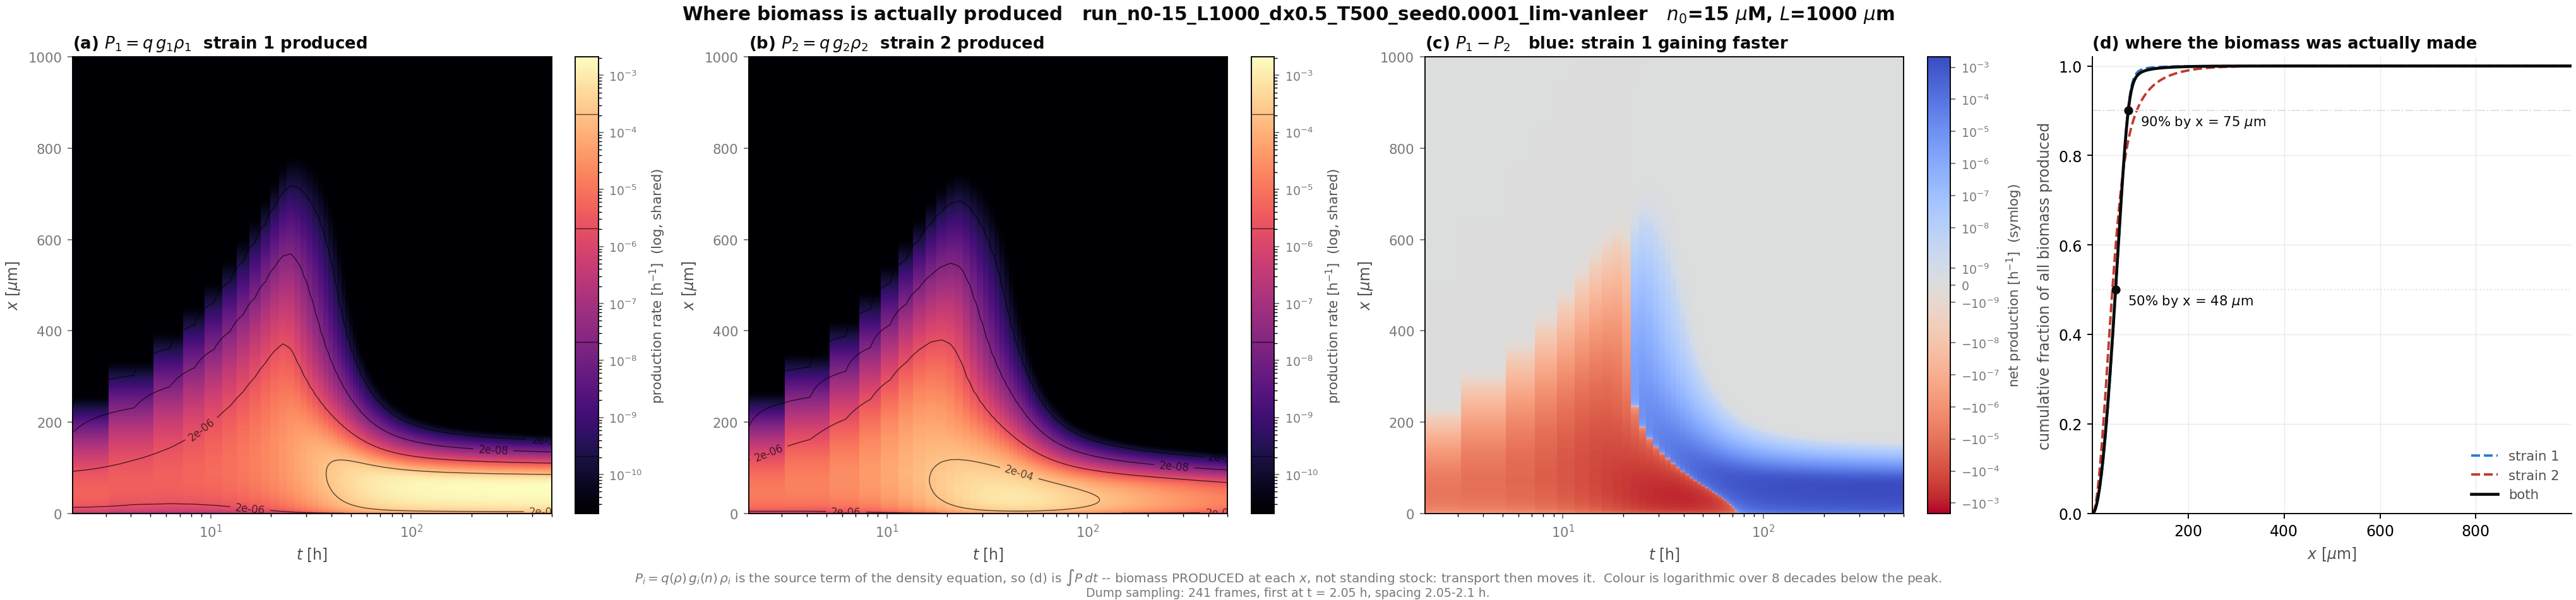
\includegraphics[width=\textwidth]{production_maps_dilute_n0-15_T500}
		\caption{Dilute, $T=500h, n_0=15 \mathrm{\mu M}$}
		\label{fig:gdil}
	\end{subfigure}
	\hfill
	\begin{subfigure}{\textwidth}
		\centering
		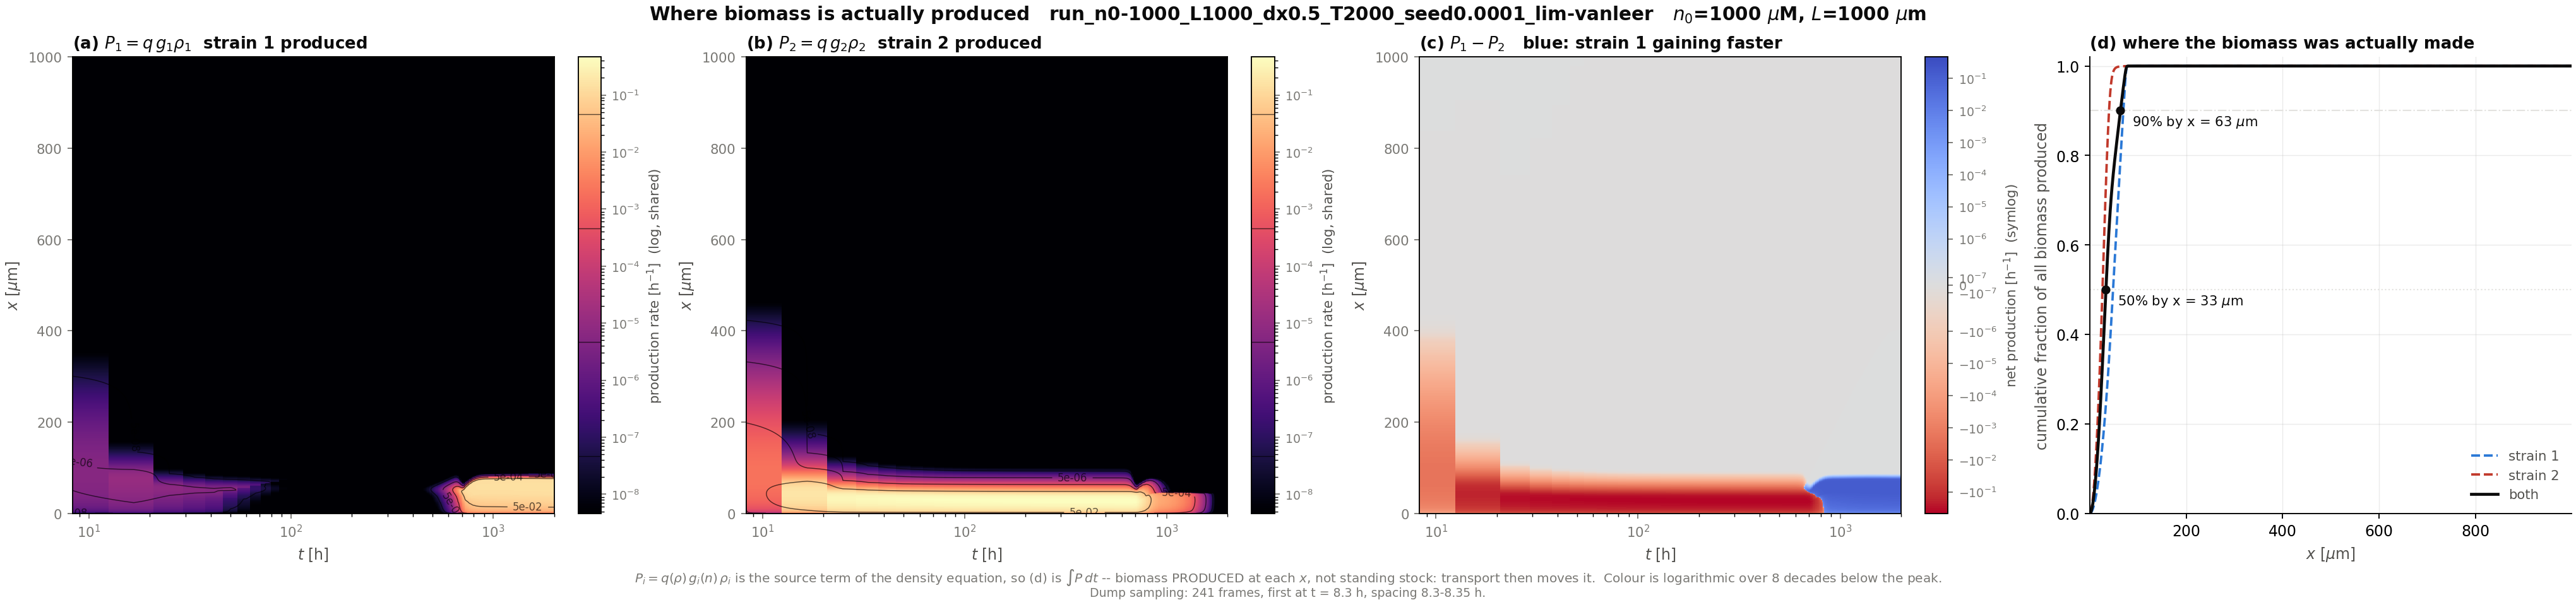
\includegraphics[width=\textwidth]{production_maps_jammed_n0-1000_T2000}
		\caption{Jammed, $T=2000h, n_0=1000 \mathrm{\mu M}$}
		\label{fig:gjam}
	\end{subfigure}
	\caption{Where biomass is actually produced, production as a heatmap over position and time. (A) Biomass production of the high affinity strain as position over time, (B) Biomass production of the glutton strain as position over time, (C) Selective production $P_1-P_2$ as position over time, (D) Production of all biomass made until final time over position.}
\end{figure}
\label{fig:g}
\FloatBarrier
But most biomass that was produced does not survive, it instead gets washed out. In the dilute case only $12.1\%$ of produced biomass actually survived until final time, while in the longer jammed case only $3.4\%$ survives. As such it is more accurate to look at the production of the surviving population. The surviving population was produced a bit further into the cavity, since if a cell was produced further from the washout opening it has a higher chance of survival.
\begin{figure}[htbp]
	\centering
	\begin{subfigure}{\textwidth}
		\centering
		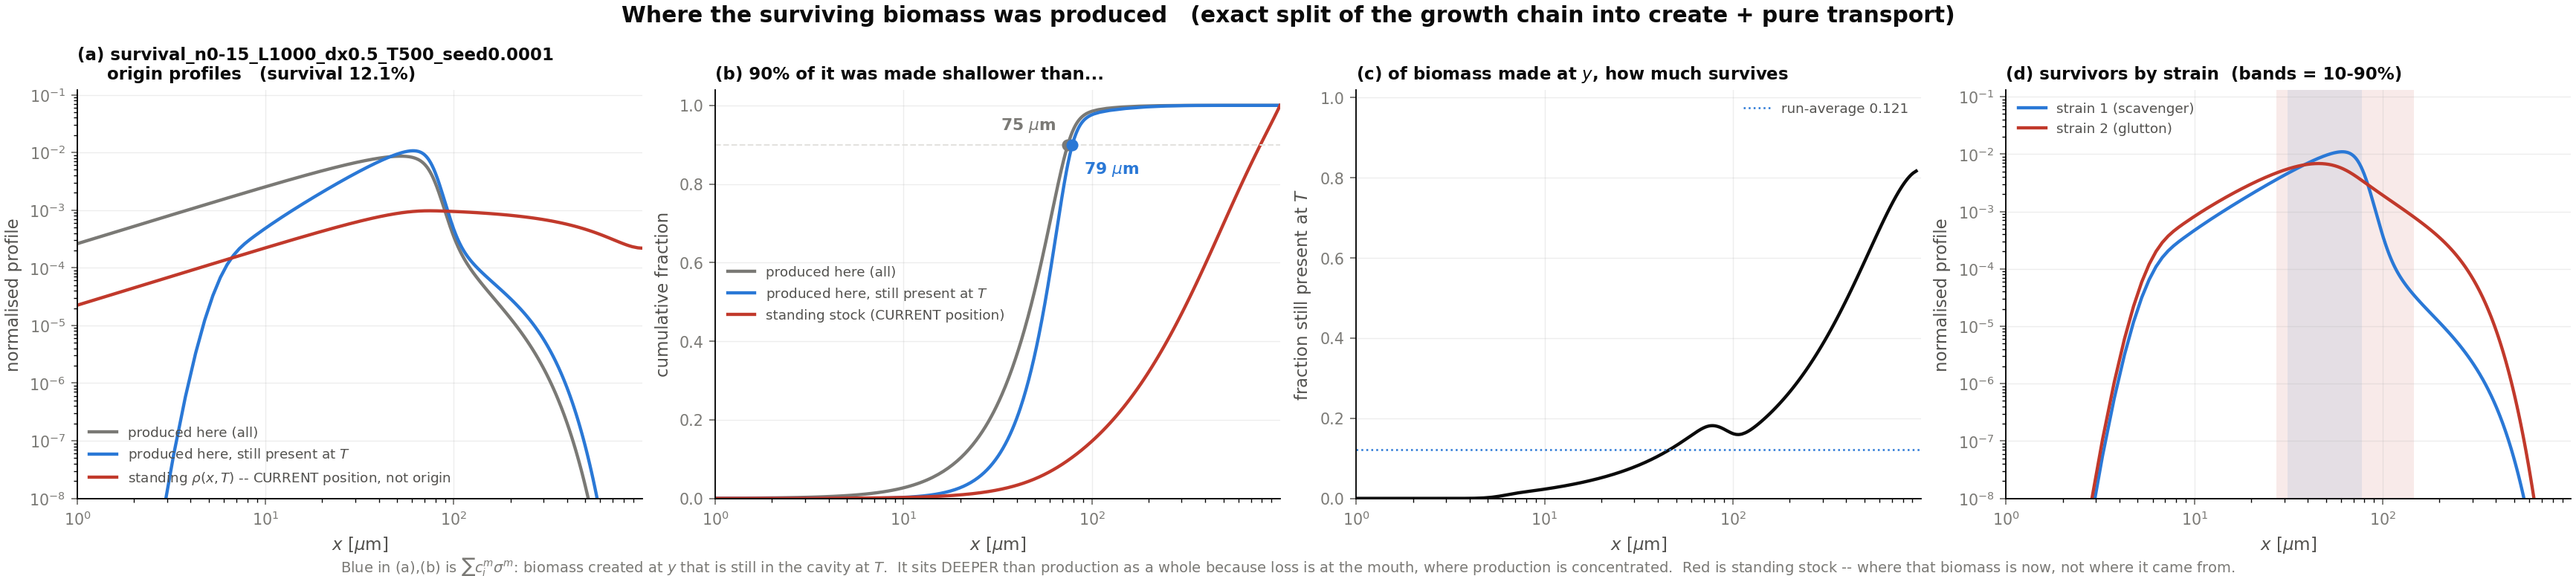
\includegraphics[width=\textwidth]{survival_origindil}
		\caption{Dilute, $T=500h, n_0=15 \mathrm{\mu M}$}
		\label{fig:survivaldil}
	\end{subfigure}
	\hfill
	\begin{subfigure}{\textwidth}
		\centering
		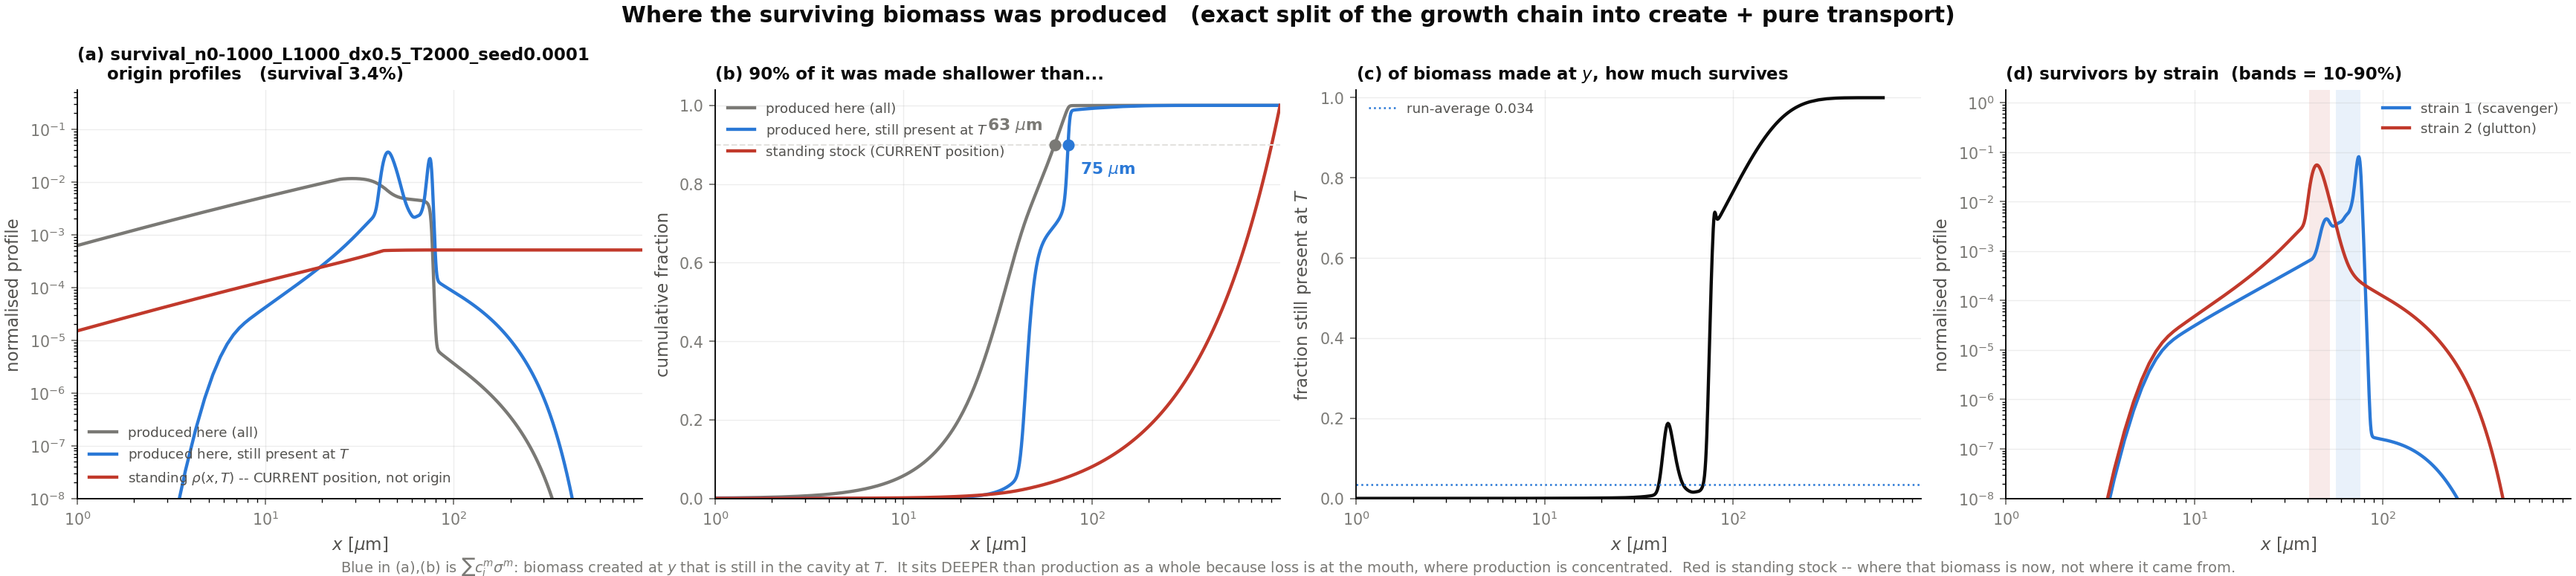
\includegraphics[width=\textwidth]{survival_originjam}
		\caption{Jammed, $T=2000h, n_0=1000 \mathrm{\mu M}$}
		\label{fig:survivaljam}
	\end{subfigure}
	\caption{In what interval was the surviving biomass produced, y-axis: how much of the population was produced from the interval from 0 to x, x-axis: position in the cavity. Grey denotes all biomass produces, blue the survivors and red the position of the current population occupying the cavity.}
\end{figure}
\label{fig:survival}
\FloatBarrier
	\chapter{Methods}
	\section{Transport closures}
	\label{transport}
	Following Slepukhin (Eq.~16)\cite{slepukhin} the collective diffusivity penalizes densities above $\rho_{\mathrm jam}$: below jamming it is the Richardson-Zaki \cite{zaki} \cite{Karita} mobility $\mu(\Phi)=\mu_0(1-\Phi)^{\eta}$ times the Carnahan-Starling equation of state for rigid hard spheres and above jamming an incompressible branch pins $\rho$ near $\rho_{\mathrm jam}$,
	\begin{equation}
		{
			D_{\rm col}(\rho)
			=
			D_0
			\frac{\mu(\Phi(\rho))\,dP(\Phi(\rho))}
			{\mu(0)\,dP(0)}
		}
		\qquad 0\le \rho<\rho_{\rm jam}.
		\label{eq:Dcol_slepukhin_closure}
	\end{equation}
	Let $D_0$ denote the dilute diffusivity, $\mu$ the collective
	mobility and $dP$ is the osmotic compressibility factor. With
	\begin{equation}
		D_{\rm col}(0)=D_0.
		\label{eq:Dcol_dilute_normalization}
	\end{equation}
	The jamming transition of hard spheres
	\begin{equation}
		dP(\Phi)
		=
		\frac{6}{\pi}A(\Phi)
		+
		\frac{6\Phi}{\pi}\partial_\Phi A(\Phi),
		\label{eq:dP_definition}
	\end{equation}
	with the Carnahan–Starling compressibility factor \cite{carnahan}
	\begin{equation}
		A(\Phi)=
		\frac{1+\Phi+\Phi^2-\Phi^3}{(1-\Phi)^3}.
		\label{eq:A_definition}
	\end{equation}
	For $\Phi=\rho$ the closure can be reduced to
	\begin{equation}
		D_{col}(\rho)=
		\begin{cases}
			D_0(1-\rho)^{\eta-4}\left(1+4\rho+4\rho^2-4\rho^3+\rho^4\right), & \rho\leq\rho_{\mathrm jam},\\[0.5em]
			1000\,D_0\,(\rho-\rho_{\mathrm jam})+D_{col}(\rho_{\mathrm jam}), & \rho>\rho_{\mathrm jam},
		\end{cases}
		\label{eq:Dcol}
	\end{equation}
	where $D_{col}(\rho_{\mathrm jam})$ is the sub-jamming value at $\rho=\rho_{\mathrm jam}$ \ref{subsec:Dcol_derivation}.
	Self diffusivity of single cells from the IBM simulation \cite{slepukhin} is adapted to our continuum model
	\begin{equation}
		D_{\rm self} = D_0
		\begin{cases}
			(1-0.95  \rho/\rho_{\rm jam}), \quad \rho<\rho_{\rm jam}\\
			1.5\times 10^{-3} , \quad \rho \ge \rho_{\rm jam}
		\end{cases}
		\label{eq:Dself}
	\end{equation}
	We define the density pressure potential as
	\begin{equation}
		\Psi(\rho):=\int_0^\rho D_{\rm col}(s)\,ds,
		\label{eq:pressure_potential_short}
	\end{equation}
	such that
	\begin{equation}
		J_\rho=-\Psi_x .
		\label{eq:pressure_flux_short}
	\end{equation}
	\begin{figure}
	\centering
	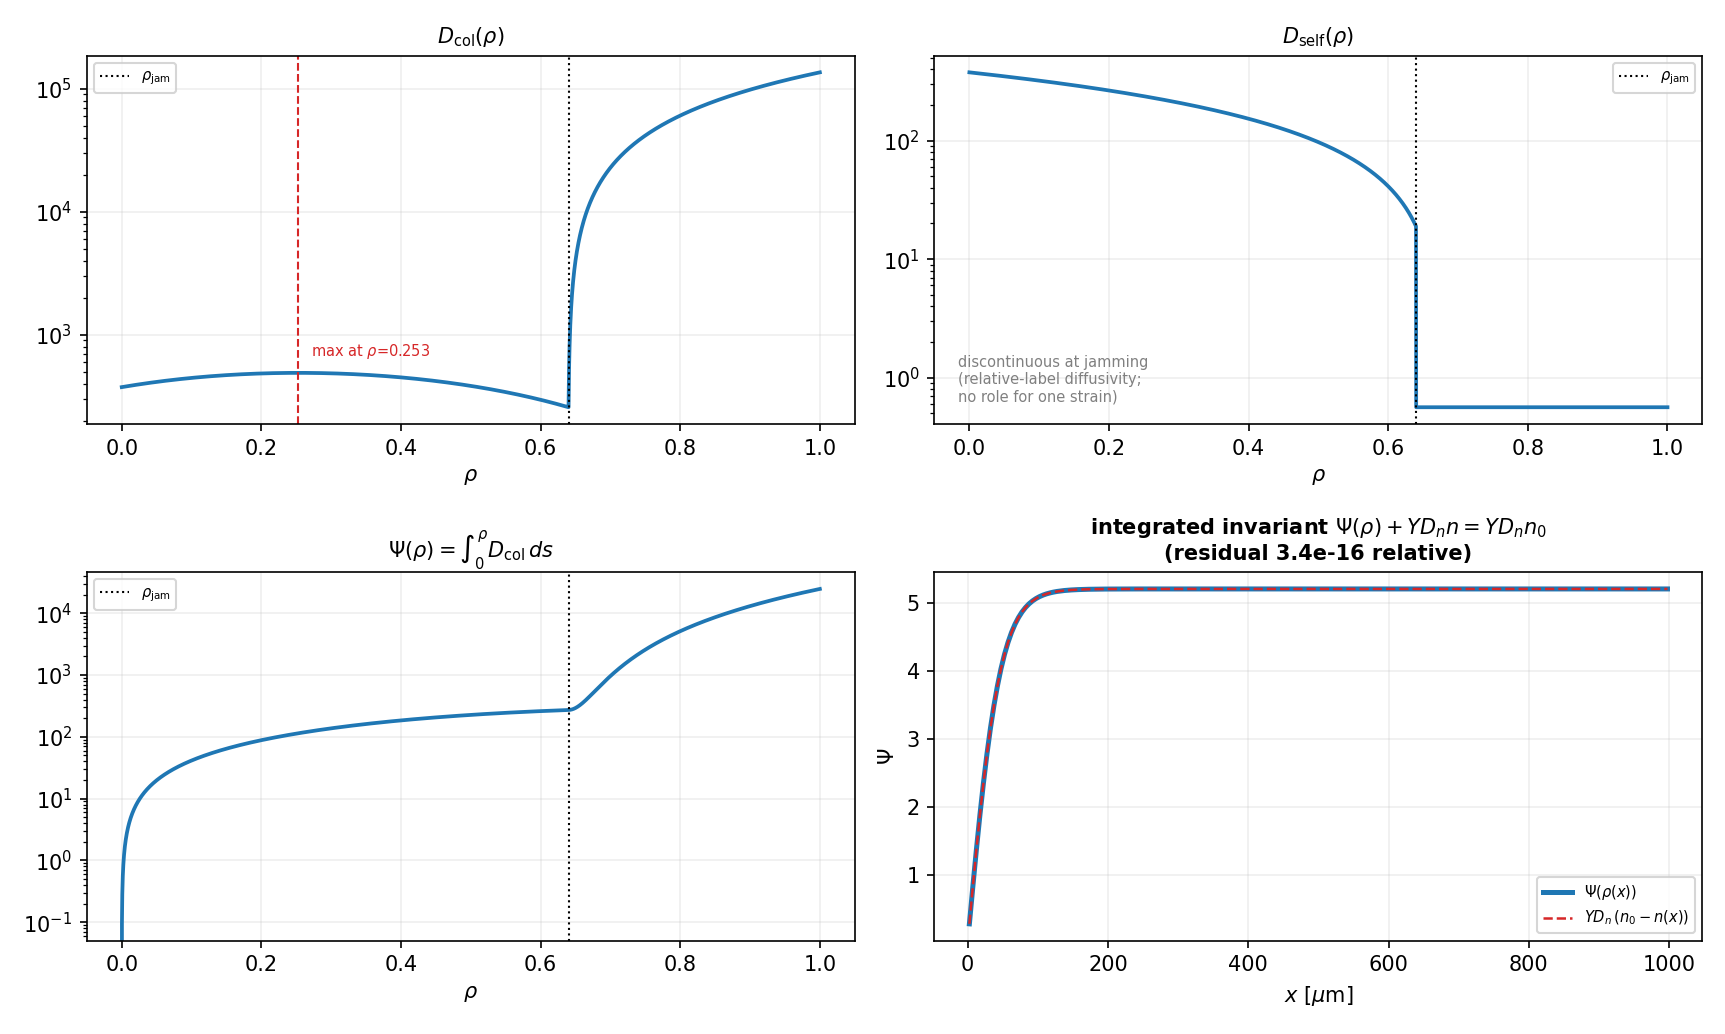
\includegraphics[width=\linewidth]{steady_closures}
	\caption{(a) Collective Diffusion shape over density, (b) Self diffusion of single cells over density, not used in the single strain problem, (c) Pressure potential as a function of density, (d) The integrated invariant in a dilute population of gluttons, i.e. strain 2 inside a 1mm long cavity.}
	\label{fig:steadyclosures}
\end{figure}
	\paragraph{Parameters}
	The random close packing value is $\Phi_{\mathrm{rcp}} \approx 64\%$ for 3D monodisperse spheres, treating cells as hard spheres of the same size. We inherit this value as the jamming transition density $\rho_{\mathrm jam}=0.64$. The mobility exponent $\eta=5.8$ was extracted by Karita numerically as a fit parameter via linear regression. The dilute diffusivity of a single cell is a measured value $D_0=376 \pm 6\,\mu\mathrm{m}^2/\mathrm{h}$. \cite{Karita}
	\paragraph{Additional assumptions}
	\begin{assumption}[Nutrient diffusion]
		There is a nutrient concentration $n(x,t)$ with flux under Ficks law \cite{Fick}
		\begin{equation}
			J_n=-D_n n_x,
			\qquad D_n=\text{const.}>0.
			\label{eq:nutrient_flux}
		\end{equation}
	\end{assumption}
	
	\begin{assumption}[Monod growth]
		Biomass grows with nutrient-dependent rate\cite{Monod}
		\begin{equation}
			g(n)=\mu_{\max}\frac{n}{K_s+n},
			\qquad \mu_{\max}>0,
			\qquad K_s>0.
			\label{eq:monod}
		\end{equation}
	\end{assumption}
	
	\begin{assumption}[Yield-coupled nutrient consumption]
		Nutrient is consumed in proportion to biomass production, with constant yield $Y>0$ \cite{Monod}. Thus the nutrient sink is
		\begin{equation}
			\frac{1}{Y}g(n)\rho.
			\label{eq:yield_sink}
		\end{equation}
	\end{assumption}
	
	\begin{assumption}[No nutrient-dependent mechanics]
		Growth and consumption are nutrient dependent but the collective diffusion remain only density dependent
		\begin{equation}
			D_{\rm col}=D_{\rm col}(\rho),
			\qquad
			D_{\rm col}\neq D_{\rm col}(\rho,n).
		\end{equation}
	\end{assumption}
\paragraph{Monod growth for two strains and the crossing condition}	
The strains grow in accordance with the Monod growth law \cite{Monod}
\begin{equation}
	g_1(n)=\mu_1\frac{n}{K_1+n},
	\qquad
	g_2(n)=\mu_2\frac{n}{K_2+n}.
\end{equation}
The local selection coefficient is
\begin{equation}
	s(n)=g_1(n)-g_2(n).
	\label{eq:selection-def}
\end{equation}
For \(n>0\) the crossing \(s(n^*)=0\) is determined by
\begin{equation}
	n^*=\frac{\mu_1K_2-
		\mu_2K_1}{\mu_2-
		\mu_1}.
	\label{eq:monod-crossing}
\end{equation}
When \(\mu_2>\mu_1\) and \(\mu_1/K_1>\mu_2/K_2\), strain 1 is locally growth favored at low nutrient (scavenger/high affinity) and strain 2 at high nutrient (glutton). As such for our E. coli strain growth functions cross at $n^*\approx5.25 \mathrm{\mu M}$ \ref{sec:ecoli}, making it a model of specialist resource competition.
\section{Pressure plane reduction}
\label{plane}
Similarly to how Karita \cite{Karita} calculated the cavity length for a phase diagram, we can derive a threshold cavity length. Meaning for a given $n_*$ or equivalently $\rho_*$ we know how long the cavity needs to be at minimum to reach it or vice versa.
Let
\begin{equation}
	p:=\Psi(\rho),
	\qquad
	q:=p_x=\Psi_x=D_{\rm col}(\rho)\rho_x.
\end{equation}
Then the steady state biomass equation is
\begin{equation}
	q_x=-g(n)\rho.
\end{equation}
Since $p_x=\Psi_x=-YD_n n_x\ge 0$ along every admissible steady state,
$p$ is monotone along the profile. So $p$ can be used as the trajectory
variable and we can write $q=q(p)$ and $p_x=q$,
\begin{equation}
	q_x=\frac{dq}{dp}p_x=q\frac{dq}{dp}.
\end{equation}
so
\begin{equation}
	{
		q\frac{dq}{dp}=-g(n(p))\rho(p).
	}
	\label{eq:pressure_plane_new}
\end{equation}
The invariant gives
\begin{equation}
	{
		n(p)=n_0-\frac{p}{YD_n}.
	}
	\label{eq:n_of_p_zero_opening}
\end{equation}
For the finite threshold $p_*:=\Psi(\rho_*)=YD_n(n_0-n_*)$, the bottom
no-flux condition gives
\begin{equation}
	q(p_*)=0.
\end{equation}
Integrating \eqref{eq:pressure_plane_new} from $p$ to $p_*$ gives
\begin{equation}
	{
		q^2(p)=2\int_p^{p_*}g(n(s))\rho(s)\,ds.
	}
\end{equation}
Since
\[
q=p_x=\frac{dp}{dx},
\]
we can use $p$ as the integration variable along the steady profile
\[
dx=\frac{dp}{q(p)}.
\]
At the opening,
\[
p=p_0:=\Psi(\rho_0),
\]
and at the threshold point,
\[
p=p_*:=\Psi(\rho_*).
\]
Therefore the cavity length is
\begin{align}
	L_*
	&=\int_0^{L_*} dx \\
	&=\int_{p_0}^{p_*}\frac{dp}{q(p)}.
	\label{eq:length_from_q}
\end{align}
Using
\[
q(p)
=
\sqrt{
	2\int_p^{p_*}g(n(s))\rho(s)\,ds
},
\]
So for $\rho_0=0$ the threshold length is
\begin{equation}
	{
		L_*=
		\int_0^{p_*}
		\frac{dp}{\sqrt{2\int_p^{p_*}g(n(s))\rho(s)\,ds}}.
	}
	\label{eq:Lstar_exact_new}
\end{equation}
\section{Approximations and $L^*$ in the dilute regime}
\label{dilute}
\paragraph{Closed-end density in the dilute regime}
For a prescribed nutrient threshold $n_*$, the closed-end density is
\begin{equation}
	{
		\rho(L_*)
		=
		\frac{YD_n}{D_0}(n_0-n_*).
	}
	\label{eq:rhoL_dilute_threshold}
\end{equation}
The dilute approximation is self-consistent at that threshold if
\begin{equation}
	{
		\frac{YD_n(n_0-n_*)}{D_0\rho_{\rm jam}}\ll1.
	}
	\label{eq:dilute_threshold_self_consistency}
\end{equation}
A sufficient condition for the entire dilute branch up to complete nutrient
budget exhaustion to remain dilute is
\begin{equation}
	{
		\frac{YD_n n_0}{D_0\rho_{\rm jam}}\ll1.
	}
	\label{eq:dilute_global_self_consistency}
\end{equation}
The biomass density remains small compared to the jamming density $\rho(x)\ll \rho_{\rm jam}$ for the entire cavity, so the collective diffusion is $D_{\rm col}(\rho)=D_0+O(\rho)\approx D_0$ and $\Psi(\rho)\approx D_0\rho$ to leading order. As well as \begin{equation}
	p=\Psi(\rho)=D_0\rho,
	\qquad
	\rho(p)=\frac{p}{D_0},
\end{equation}
The invariant gives 
\begin{equation}
	{
		\rho(x)=\frac{YD_n}{D_0}\bigl(n_0-n(x)\bigr).
	}
	\label{eq:dilute_rho_n}
\end{equation}
From the steady state nutrient equation
\begin{equation}
	D_n n_{xx}=\frac{1}{Y}g(n)\rho
\end{equation}
we get
\begin{equation}
	{
		n''=\frac{g(n)}{D_0}\bigl(n_0-n\bigr).
	}
	\label{eq:dilute_n_full_monod}
\end{equation}
If there is in addition also low nutrient concentration
\begin{equation}
	n\ll K_s,
	\qquad
	g(n)\approx kn,
	\qquad
	k:=\frac{\mu_{\max}}{K_s},
	\label{eq:dilute_A1}
\end{equation}
then \eqref{eq:dilute_n_full_monod} reduces to
\begin{equation}
	{
		n''=\frac{k}{D_0}n(n_0-n).
	}
	\label{eq:dilute_n_logistic}
\end{equation}

\subsubsection{The Dilute Phase Plane and Length Formula}
\label{subsec:dilute_phaseplane}

The local expansion above describes only the small amplitude region
$L\gtrsim L_{\rm onset}$.  To describe finite nutrient depletion while
remaining in the dilute collective-diffusion regime, we use the pressure-plane
reduction again with $\rho_0=0$.\\	
Under the dilute approximation
\begin{equation}
	\Psi(\rho)\approx D_0\rho.
\end{equation}
Thus
\begin{equation}
	p:=\Psi(\rho)=D_0\rho,
	\qquad
	\rho(p)=\frac{p}{D_0}.
	\label{eq:p_rho_dilute}
\end{equation}
The invariant becomes
\begin{equation}
	n(p)=n_0-\frac{p}{YD_n}.
	\label{eq:n_p_dilute_corrected}
\end{equation}
From the pressure plane quadrature the finite-threshold length is
\begin{equation}
	{
		L_*
		=
		\int_{0}^{p_*}
		\frac{dp}
		{
			\sqrt{
				\frac{2}{D_0}
				\int_p^{p_*}
				s\,
				g\!\left(
				n_0-\frac{s}{YD_n}
				\right)ds
			}
	}}
	\label{eq:Lstar_dilute_full_monod_rho0zero}
\end{equation}
with
\begin{equation}
	p_*=YD_n(n_0-n_*).
	\label{eq:pstar_dilute_rho0zero}
\end{equation}
Under $g(n)\approx kn$ we get
\begin{equation}
	q^2(p)
	=
	\frac{2k}{D_0}
	\int_p^{p_*}
	\left(n_0-\frac{s}{YD_n}\right)s\,ds.
\end{equation}
Evaluating the integral gives
\begin{equation}
	\int_p^{p_*}
	\left(n_0-\frac{s}{YD_n}\right)s\,ds
	=
	\frac{n_0}{2}(p_*^2-p^2)
	-
	\frac{1}{3YD_n}(p_*^3-p^3),
\end{equation}
The length formula follows
from
\[
L_*=\int_0^{p_*}\frac{dp}{q(p)}.
\]
\begin{equation}
	{
		q^2(p)
		=
		\frac{2k}{D_0}
		\left[
		\frac{n_0}{2}(p_*^2-p^2)
		-
		\frac{1}{3YD_n}(p_*^3-p^3)
		\right],
	}
	\label{eq:q2_dilute_linear_monod}
\end{equation}
and
\begin{equation}
	{
		L_*
		=
		\int_0^{p_*}
		\frac{dp}
		{
			\sqrt{
				\frac{2k}{D_0}
				\left[
				\frac{n_0}{2}(p_*^2-p^2)
				-
				\frac{1}{3YD_n}(p_*^3-p^3)
				\right]
			}
		}.
	}
	\label{eq:Lstar_dilute_linear_monod}
\end{equation}
	\section{Tipping points and window width}
\label{sec:tipping}
It has previously been demonstrated qualitatively that growth saturation can lead to the breakdown of the fold and thus a continuous jamming transition \cite{peris}. It is however decisively not a transcritical bifurcation, since there is no exchange of stability between crossing branches. The $L(\rho)$ function collapses to a vertical section, two folds annihilating each other to form a monotone branch is a cusp.
At fixed $n_0$ \eqref{eq:Lstar_exact_new} is a map $p_*\mapsto L_*(p_*;n_0)$ with the inverse being the branch of \cref{fig:steadyfold}(a).  This is the sojourn time reduction Karita \cite{Karita} (eq. 31) use to compute their phase diagram with the potential $U(p)=\int_0^pg(n(s))\rho(s)\dd s$.
The fold appears due to the falling section in the non-monotone collective diffusion function. In their constant growth model a fold either exists or does not exist, nutrient limitation can quantify when the fold is born. A tipping point is $\pd L_*/\pd\rho_*=0$, the two tipping points merge when $\frac{\partial^2 L_*}{\partial \rho_*^2}=0$ and the solution
$(\rho_c,n_0^{*})$ is the cusp. Setting $u:=\rho_*-\rho_c$ and $n_0-n_0^{*}$, which is where these two equations are satisfied. We get to the leading order \cref{app:cusp_algebra}
\begin{equation}
	\frac{\pd L_*}{\pd\rho_*}
	=c_1\bigl(n_0-n_0^{*}\bigr)+\tfrac12c_3u^2
	+O\!\bigl((n_0-n_0^{*})^2,\;u\,(n_0-n_0^{*}),\;u^3\bigr),
	\qquad
	c_1:=\frac{\pd^2L_*}{\pd\rho_*\pd n_0},
	\qquad
	c_3:=\frac{\pd^3L_*}{\pd\rho_*^3},
	\label{eq:cusp_expansion}
\end{equation}
both evaluated at the cusp. The two terms balance for
$u=O\bigl((n_0-n_0^{*})^{1/2}\bigr)$, which makes the neglected ones
$O\bigl((n_0-n_0^{*})^{3/2}\bigr)$.
\begin{equation}
	u_{\pm}=\pm\sqrt{\kappa(n_0-n_0^{*})},
	\qquad
	\kappa:=-\frac{2c_1}{c_3},
	\qquad
	\Delta\rho_*=2\sqrt{\kappa}\,\bigl(n_0-n_0^{*}\bigr)^{1/2},
	\label{eq:cusp_separation}
\end{equation}
which exist only for $\kappa(n_0-n_0^*)>0$, the fold is one-sided in $n_0$. To this
order $\pd L_*/\pd\rho_*=\tfrac12c_3(u-u_-)(u-u_+)$ and since
$\int_a^b(u-a)(u-b)\dd u=-(b-a)^3/6$ the multi valued window follows
\begin{equation}
	\Delta L=-\int_{u_-}^{u_+}L_*'\dd u=\frac{c_3}{12}\bigl(\Delta\rho_*\bigr)^3
	=\frac{2c_3}{3}\kappa^{3/2}\bigl(n_0-n_0^{*}\bigr)^{3/2}.
	\label{eq:cusp_window}
\end{equation}
substituting \eqref{eq:cusp_separation} in \eqref{eq:cusp_window} leaves $\Delta L=(c_3/12)(\Delta\rho_*)^3$, i.e. the ratio of the two exponents is $3$. Solving the cusp conditions on \eqref{eq:Lstar_exact_new} by quadrature gives
\begin{equation}
	n_0^{*}=896.16\,\mathrm{\mu M},
	\qquad
	\rho_c=0.5710=0.892\,\rhojam,
	\qquad
	L_{\rm cusp}=38.87\,\mathrm{\mu m},
	\label{eq:cusp_values}
\end{equation}
with $c_1=-4.181\times10^{-2}$, $c_3=2.673\times10^{2}$ and
$\kappa=3.129\times10^{-4}$. \begin{equation}
	\Delta\rho_*=0.0354\,\bigl(n_0-n_0^{*}\bigr)^{1/2},
	\qquad
	\Delta L=9.86\times10^{-4}\,\bigl(n_0-n_0^{*}\bigr)^{3/2},
\end{equation}
The fold is thus born below jamming, at $89\%$ of the jamming density
$\rhojam$, inside the interval where $\Dcol$ is decreasing.
\section{Dependence of inverse sorting on initial conditions}
\label{dependence}
A de novo cavity invasion through the opening is implemented by seeding the density as a gaussian distribution centered at $x=25 \mathrm{\mu m}$ with a standard deviation of $x=20 \mathrm{\mu m}$. So the initial condition for the density is
$\rho(x, t=0) = \rho_{\mathrm{seed}}\exp\left[-\frac{1}{2}\left(\frac{x-25}{20}\right)^2\right]$. The main simulations use $\rho_{\mathrm{seed}}=0.0001$, which equivalent to roughly 7 cells \cref{sec:extinction} in total and both strains equally seeded. So comfortably above the extinction threshold, since our model is continuum, meaning cells are not treated individually, seeding half a cell is not problematic since the simulation will continuously produce fractional cells either way. 
\begin{figure}
	\centering
	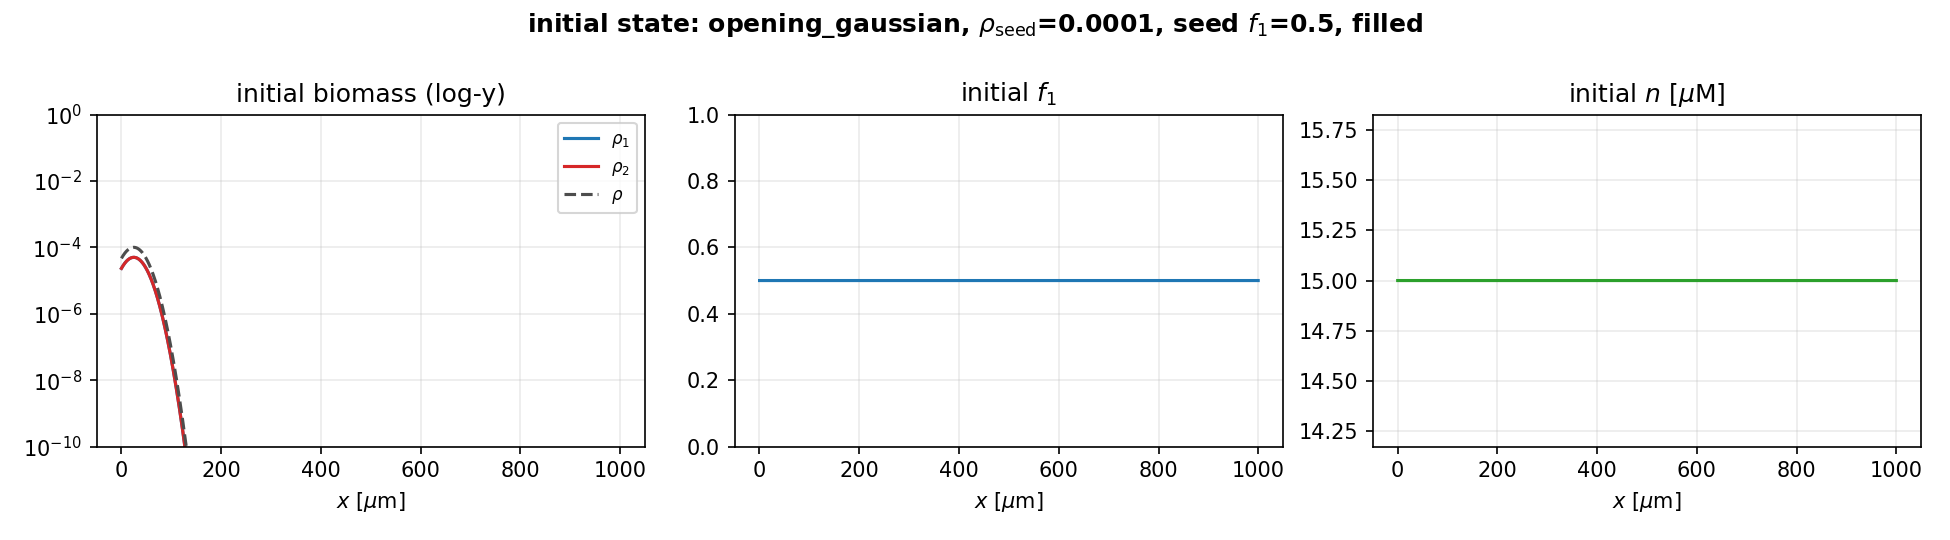
\includegraphics[width=\linewidth]{frame_000000}
	\caption{Initial profiles, showing the initial conditions for our main runs.}
	\label{fig:frame000000}
\end{figure}

\begin{figure}[htbp]
	\centering
	
	\begin{subfigure}{0.45\textwidth}
		\centering
		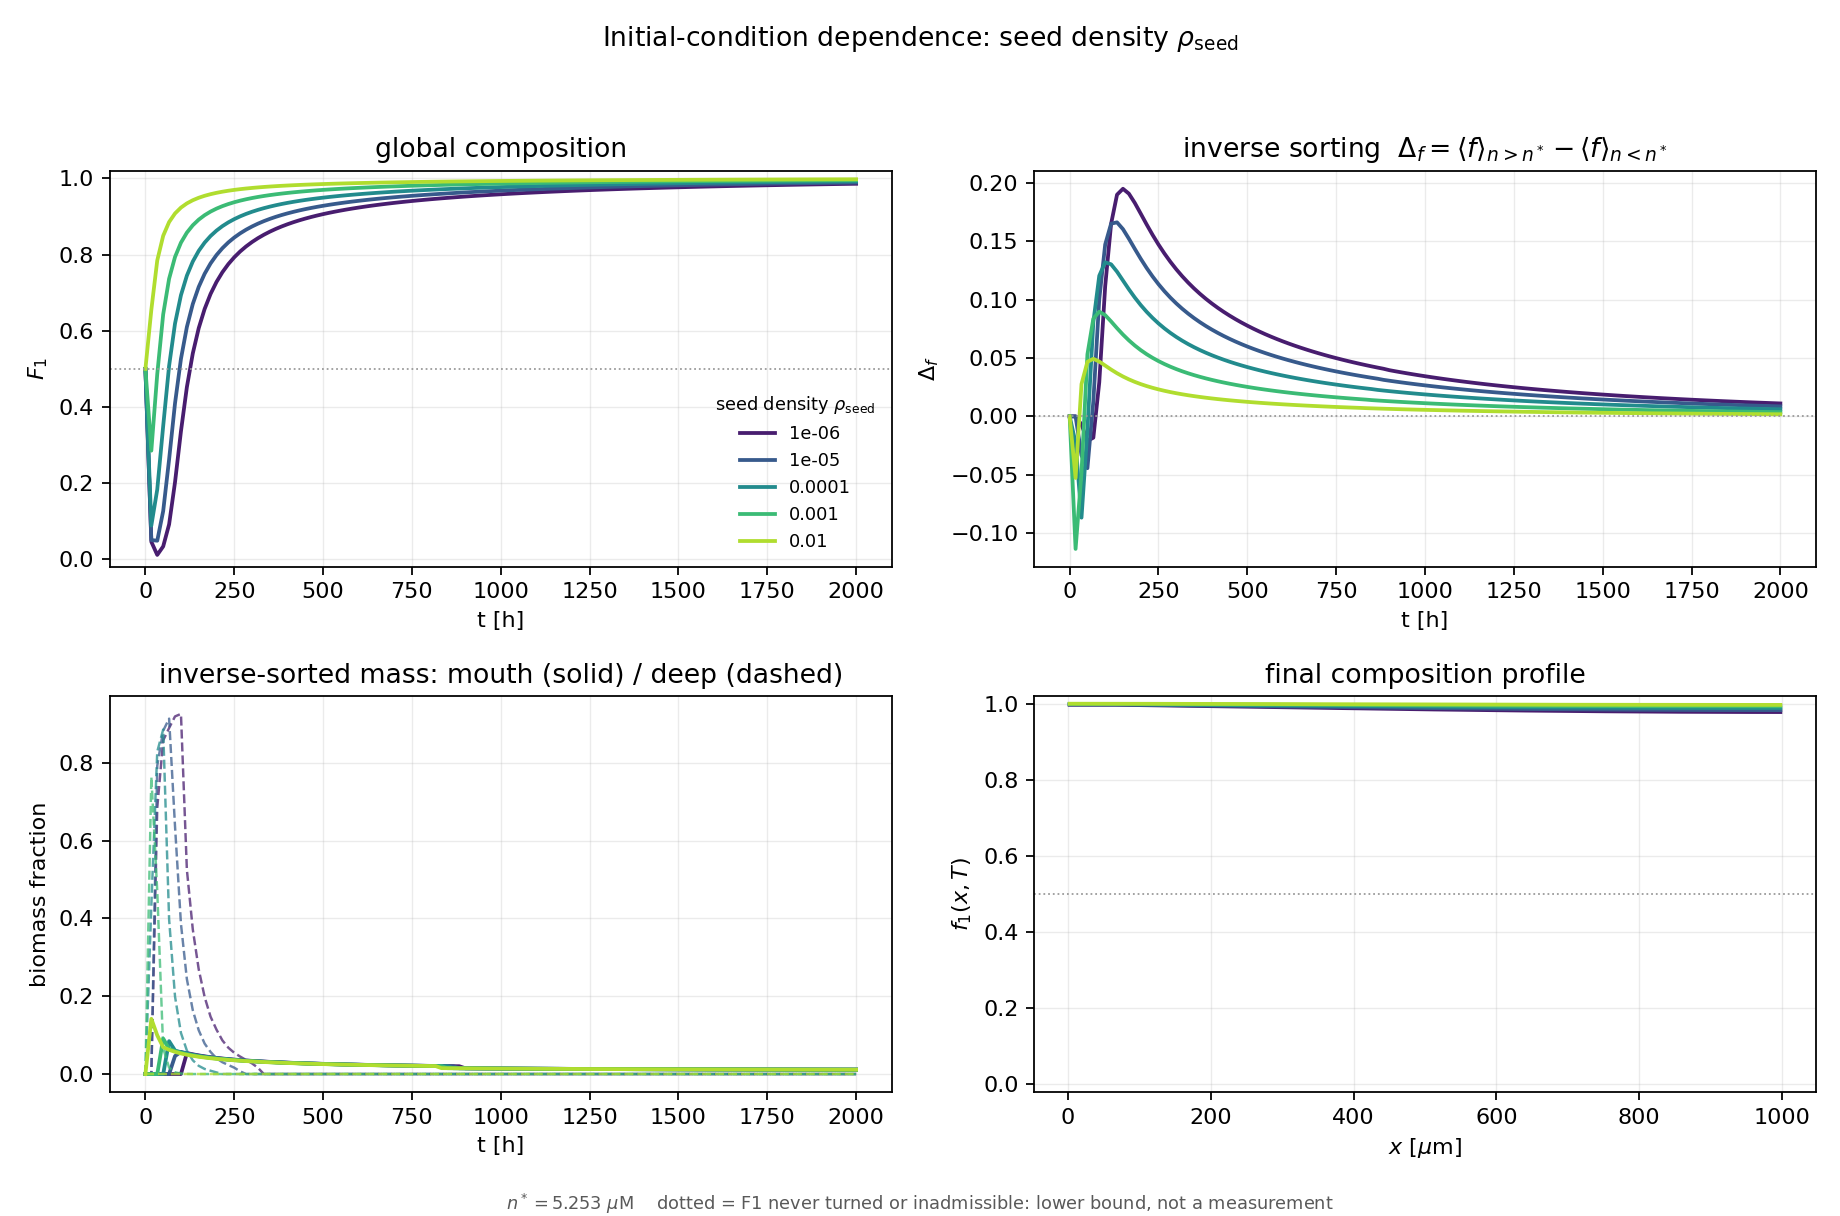
\includegraphics[width=\textwidth]{ic_density}
		\caption{Dilute}
		\label{fig:dilutedensity}
	\end{subfigure}
	\hfill
	\begin{subfigure}{0.45\textwidth}
		\centering
		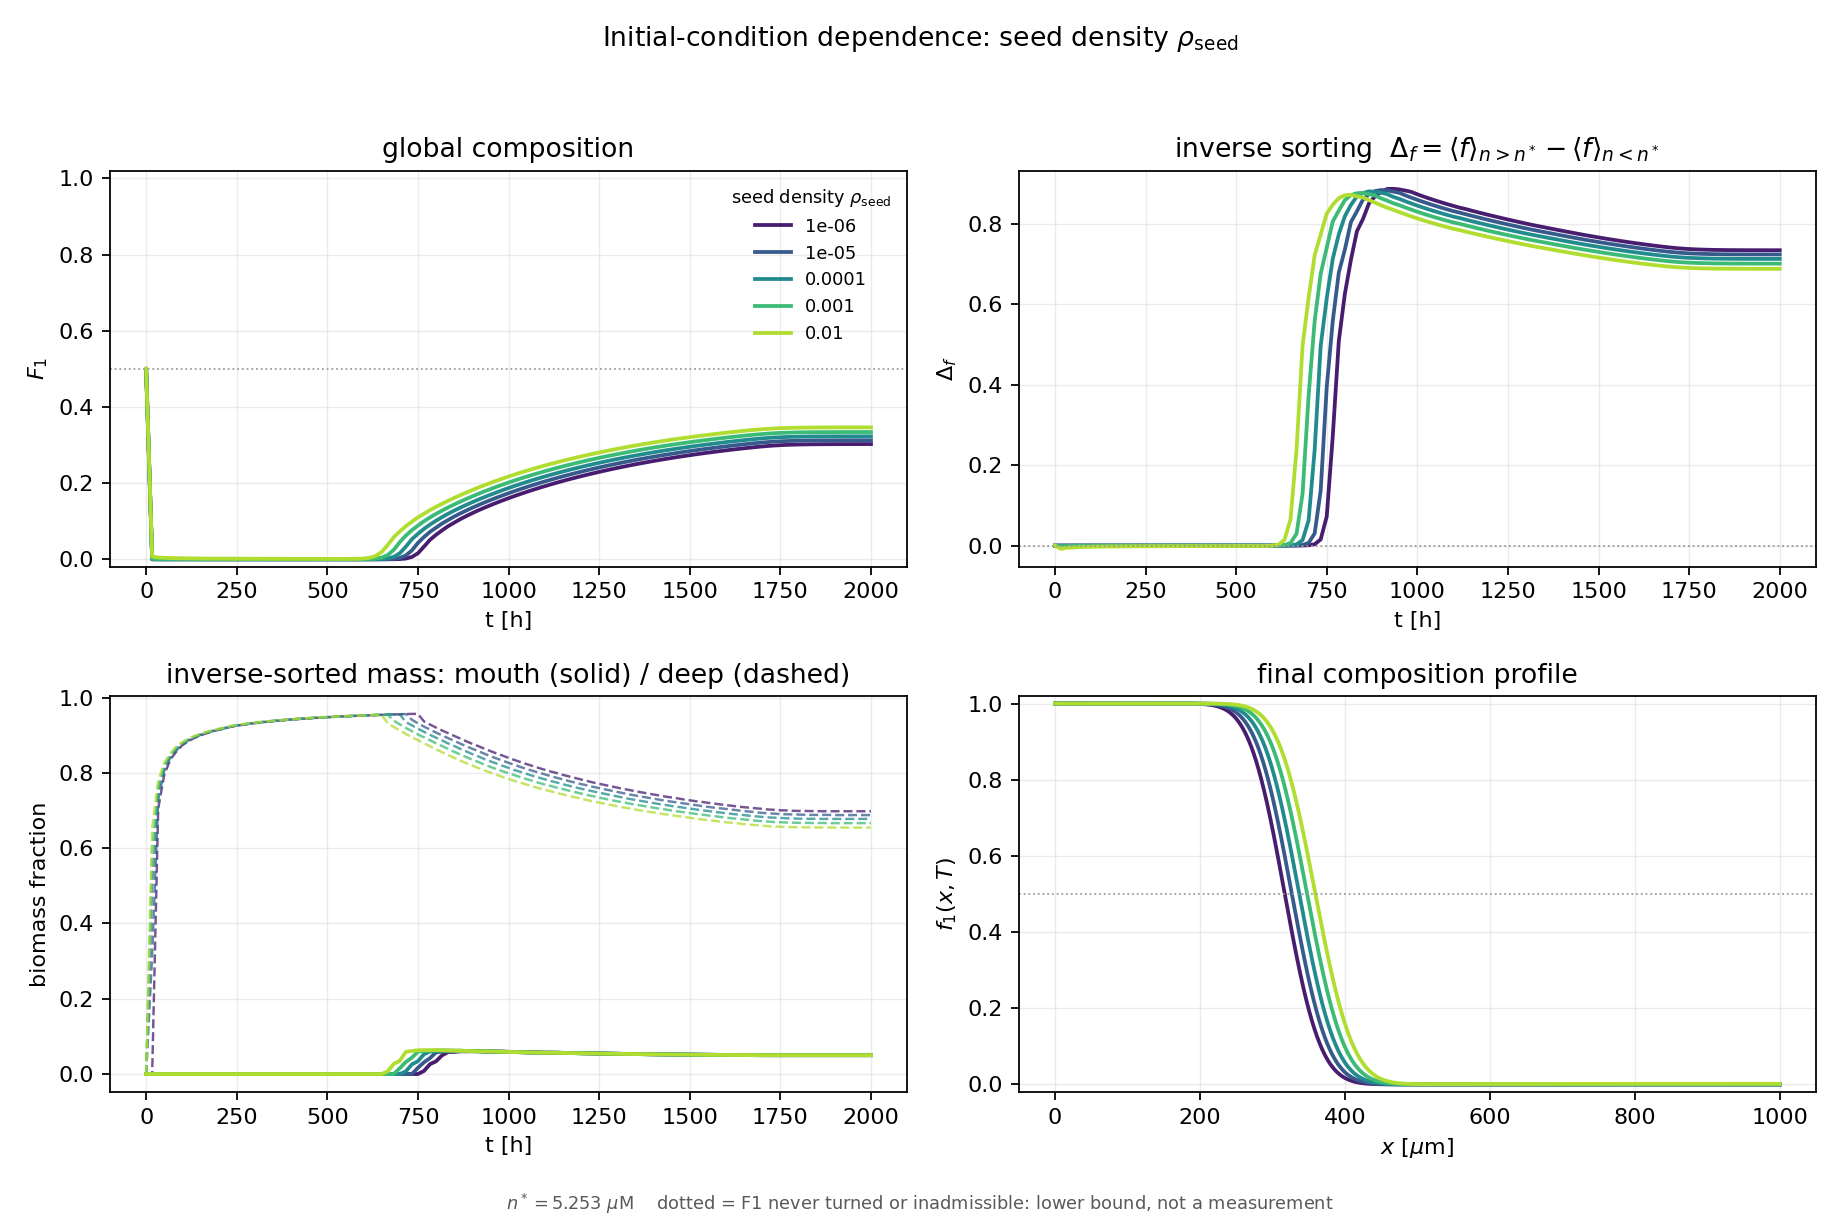
\includegraphics[width=\textwidth]{ic_density_jam}
		\caption{Jammed}
		\label{fig:jamdensity}
	\end{subfigure}
	\caption{Biomass seed of varying sizes in the invasion setting, (A) effect on global strain fraction $F1$, (B) how inverse sorting changes, (C) Split on mouth vs deep inverse sorting, (D) final profile at $T=2000h$.}
	\label{fig:seeddensity}
\end{figure}
\begin{figure}[htbp]
	\centering
	
	\begin{subfigure}{0.45\textwidth}
		\centering
		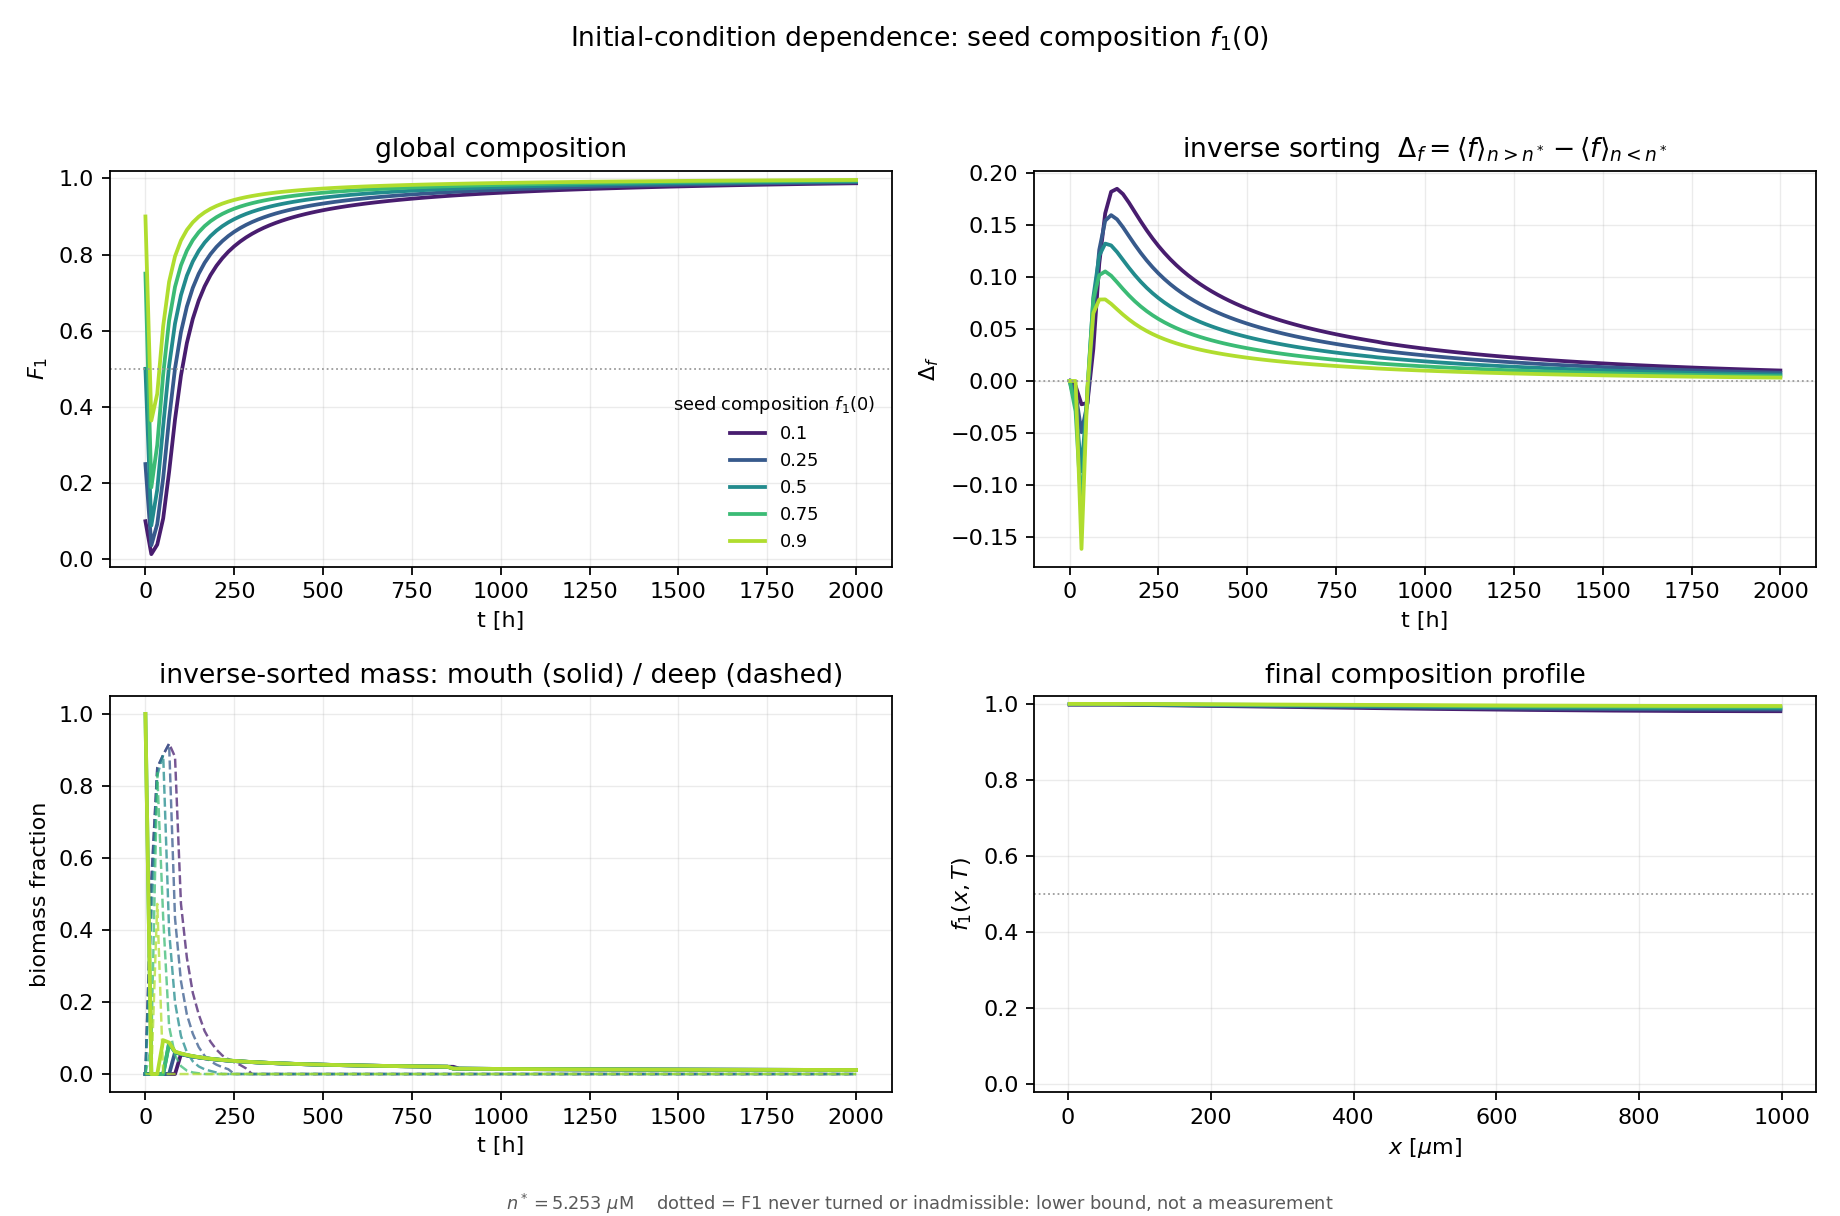
\includegraphics[width=\textwidth]{ic_f1}
		\caption{Dilute}
		\label{fig:dilutef1}
	\end{subfigure}
	\hfill
	\begin{subfigure}{0.45\textwidth}
		\centering
		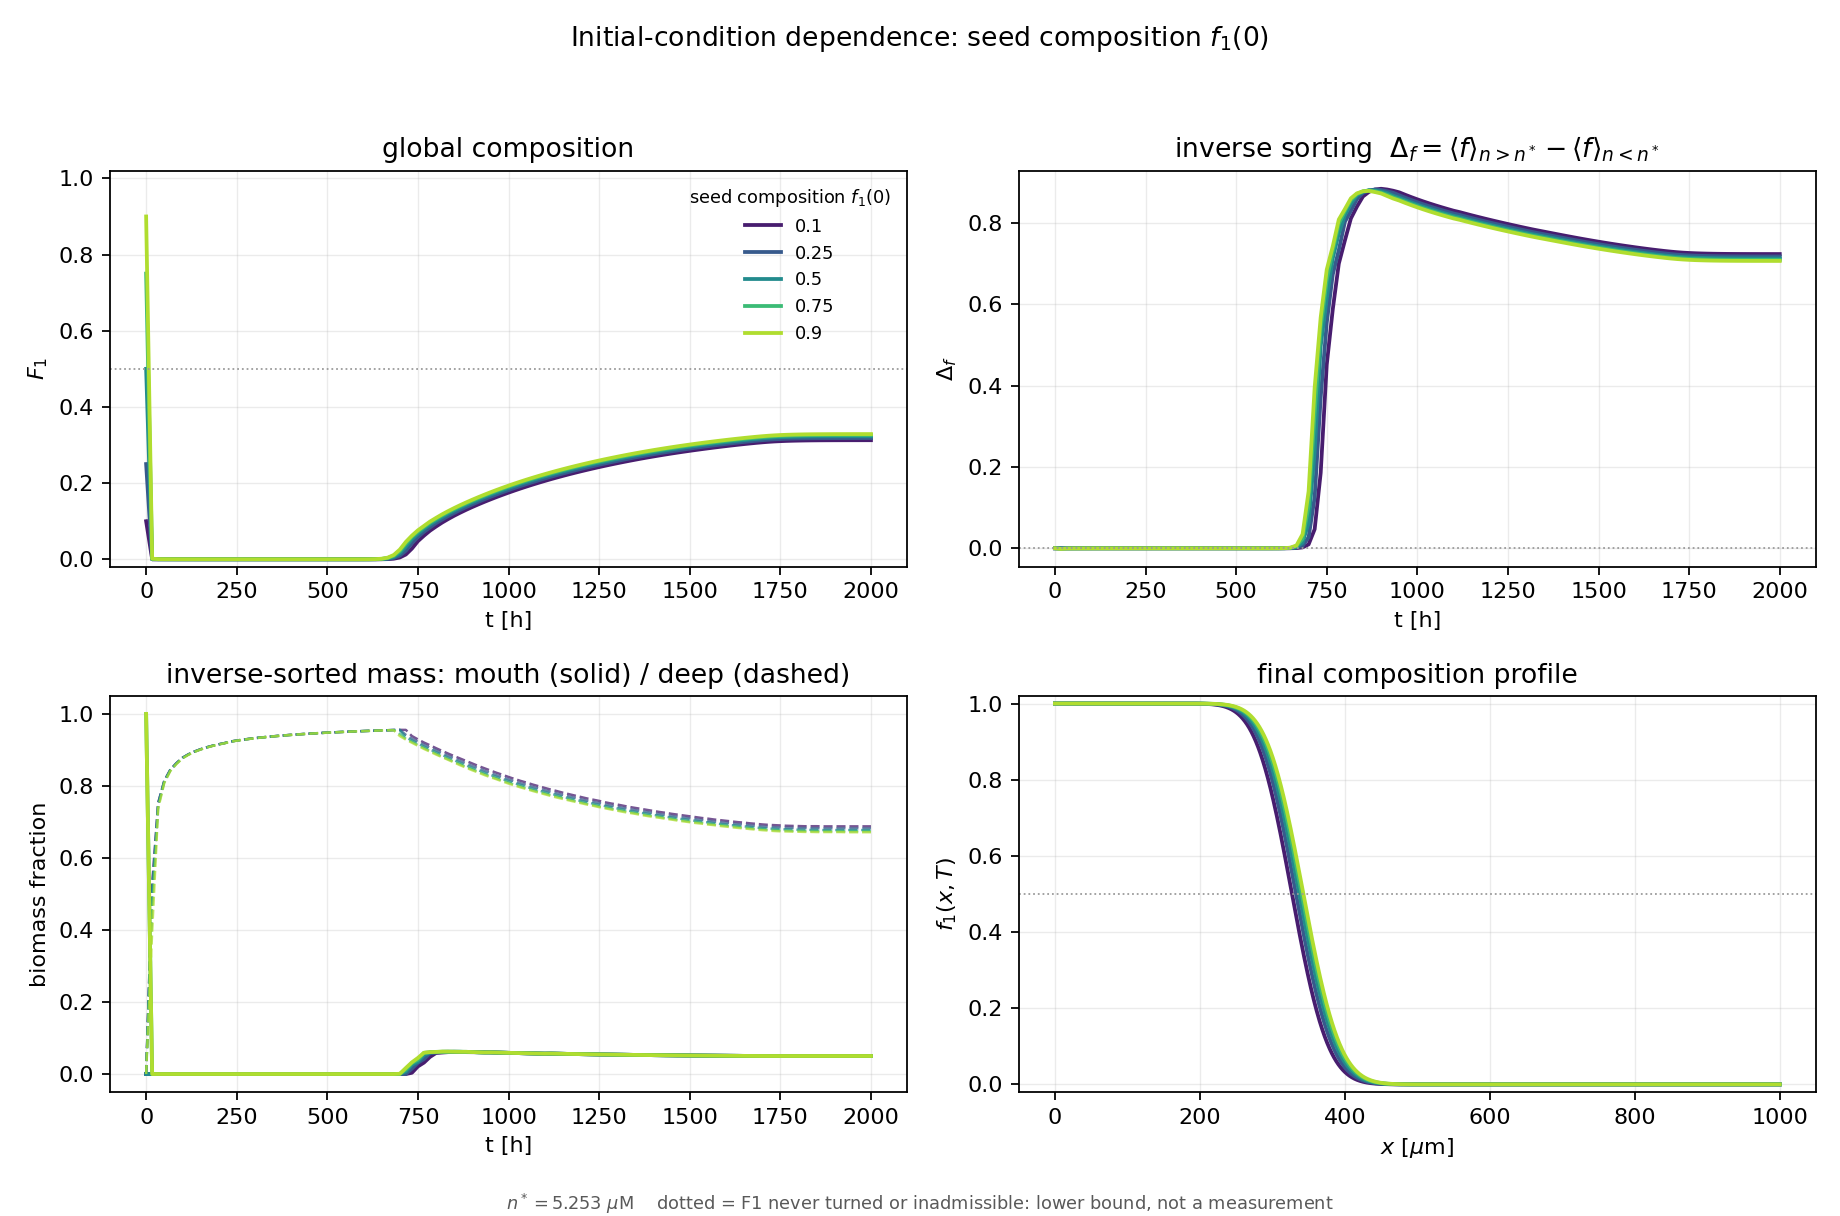
\includegraphics[width=\textwidth]{ic_f1_jam}
		\caption{Jammed}
		\label{fig:jamf1}
	\end{subfigure}
	\caption{Biomass seed of varying initial strain mixes in the invasion setting, (A) effect on global strain fraction $F1$, (B) how inverse sorting changes, (C) Split on mouth vs deep inverse sorting, (D) final profile at $T=2000h$.}
	\label{fig:seedf1}
\end{figure}
\begin{figure}[htbp]
	\centering
	
	\begin{subfigure}{0.45\textwidth}
		\centering
		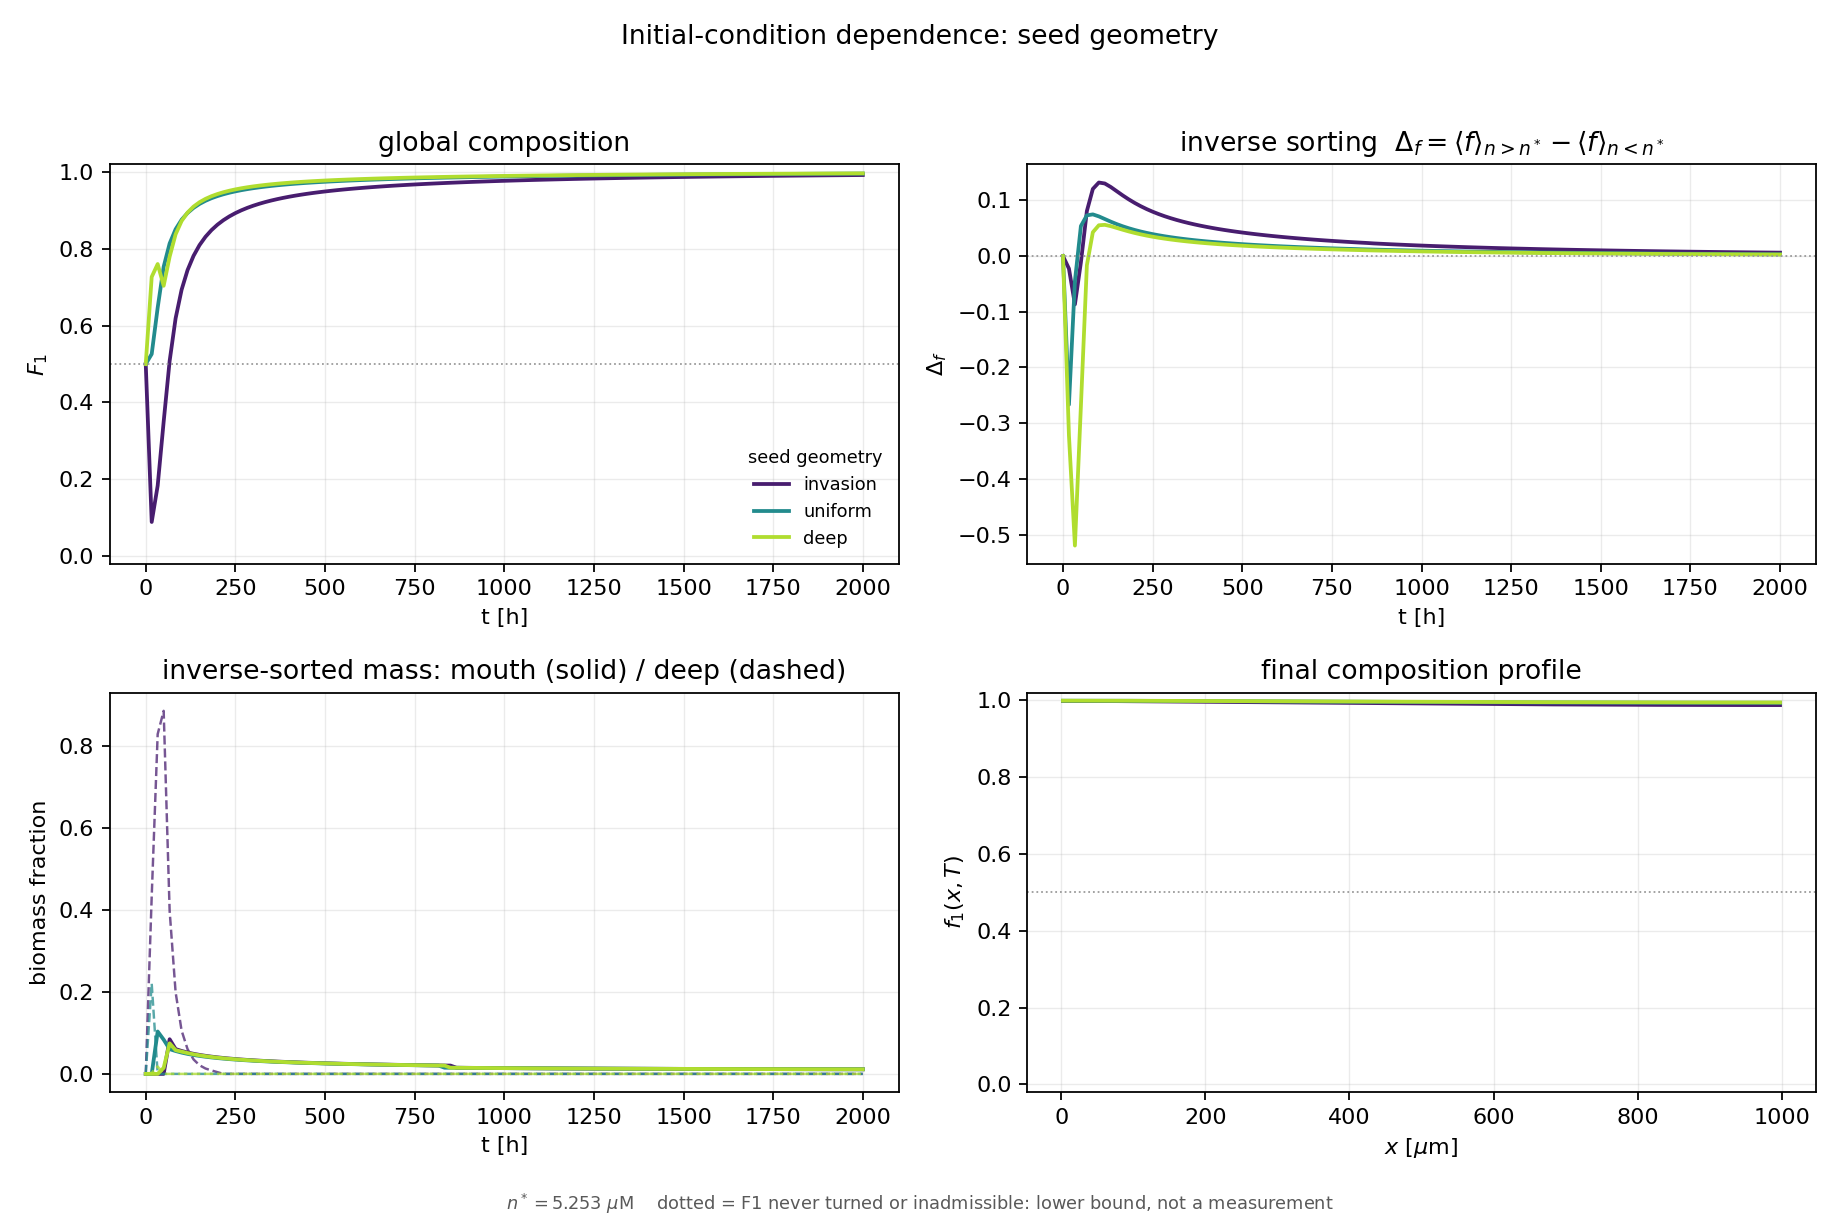
\includegraphics[width=\textwidth]{ic_mode}
		\caption{Dilute}
		\label{fig:dilutemode}
	\end{subfigure}
	\hfill
	\begin{subfigure}{0.45\textwidth}
		\centering
		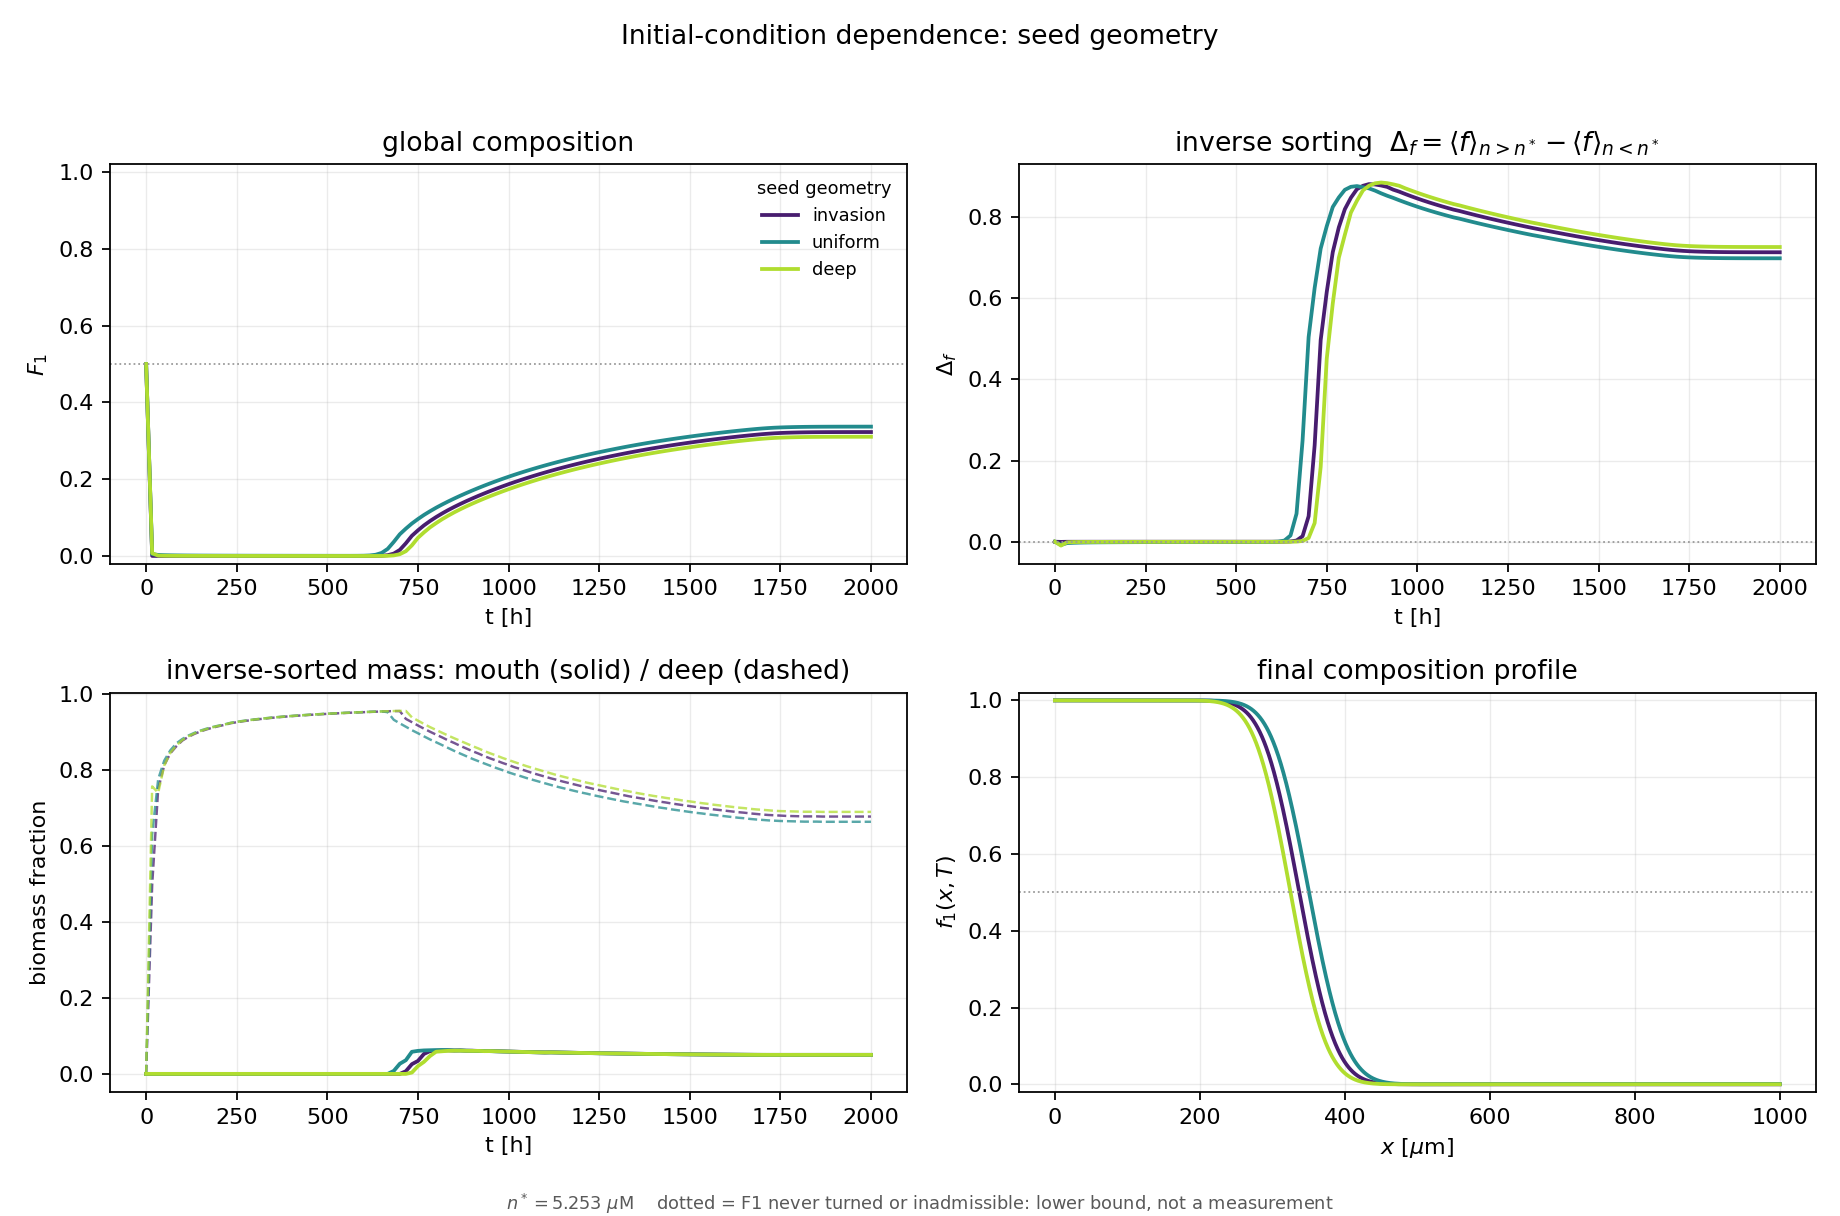
\includegraphics[width=\textwidth]{ic_mode_jam}
		\caption{Jammed}
		\label{fig:jammode}
	\end{subfigure}
	\caption{Biomass seed of varying initial setting, invasion, uniform distribution across the cavity and a seed at the deep end (A) effect on global strain fraction $F1$, (B) how inverse sorting changes, (C) Split on mouth vs deep inverse sorting, (D) final profile at $T=2000h$.}
	\label{fig:seedmode}
\end{figure}
\begin{figure}[htbp]
	\centering
	
	\begin{subfigure}{0.45\textwidth}
		\centering
		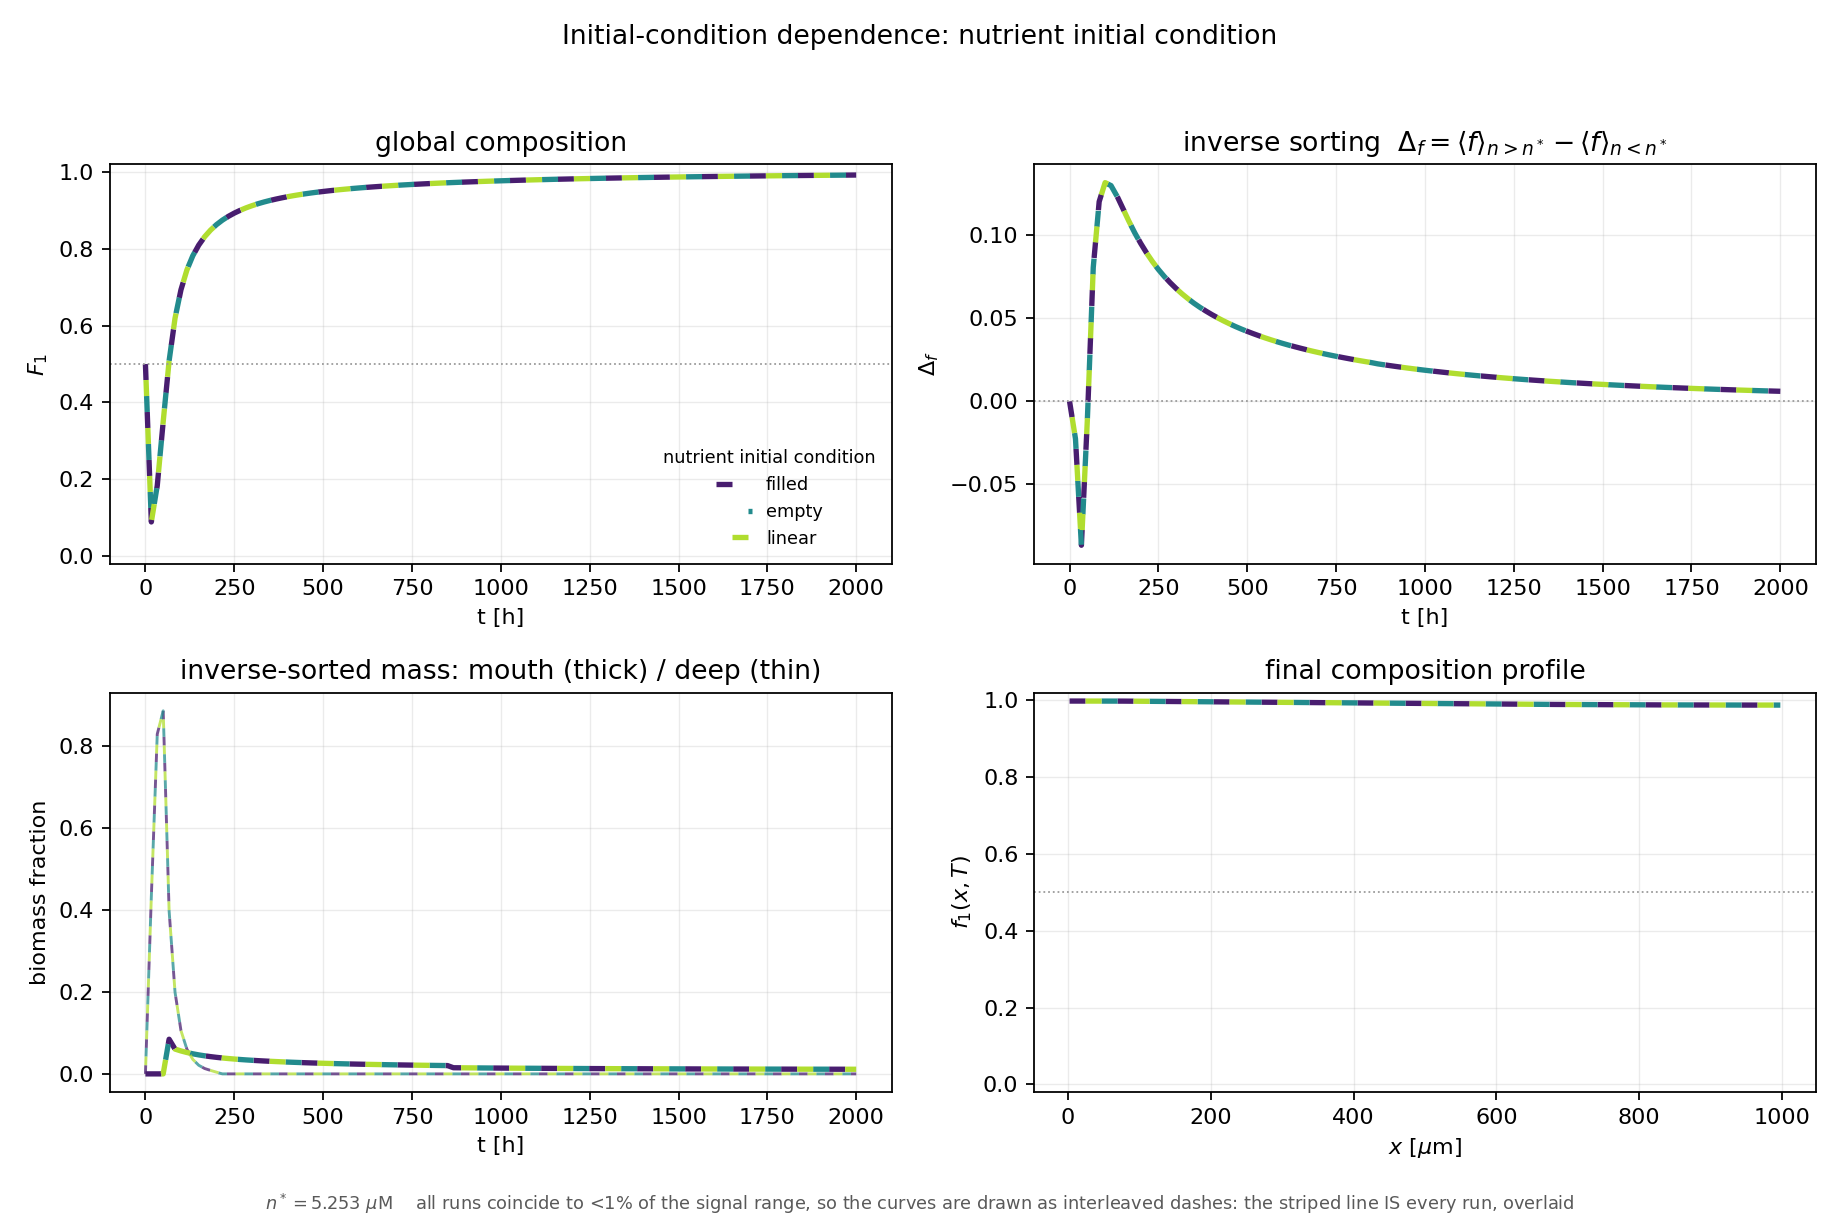
\includegraphics[width=\textwidth]{ic_nutrient}
		\caption{Dilute}
		\label{fig:diluteic}
	\end{subfigure}
	\hfill
	\begin{subfigure}{0.45\textwidth}
		\centering
		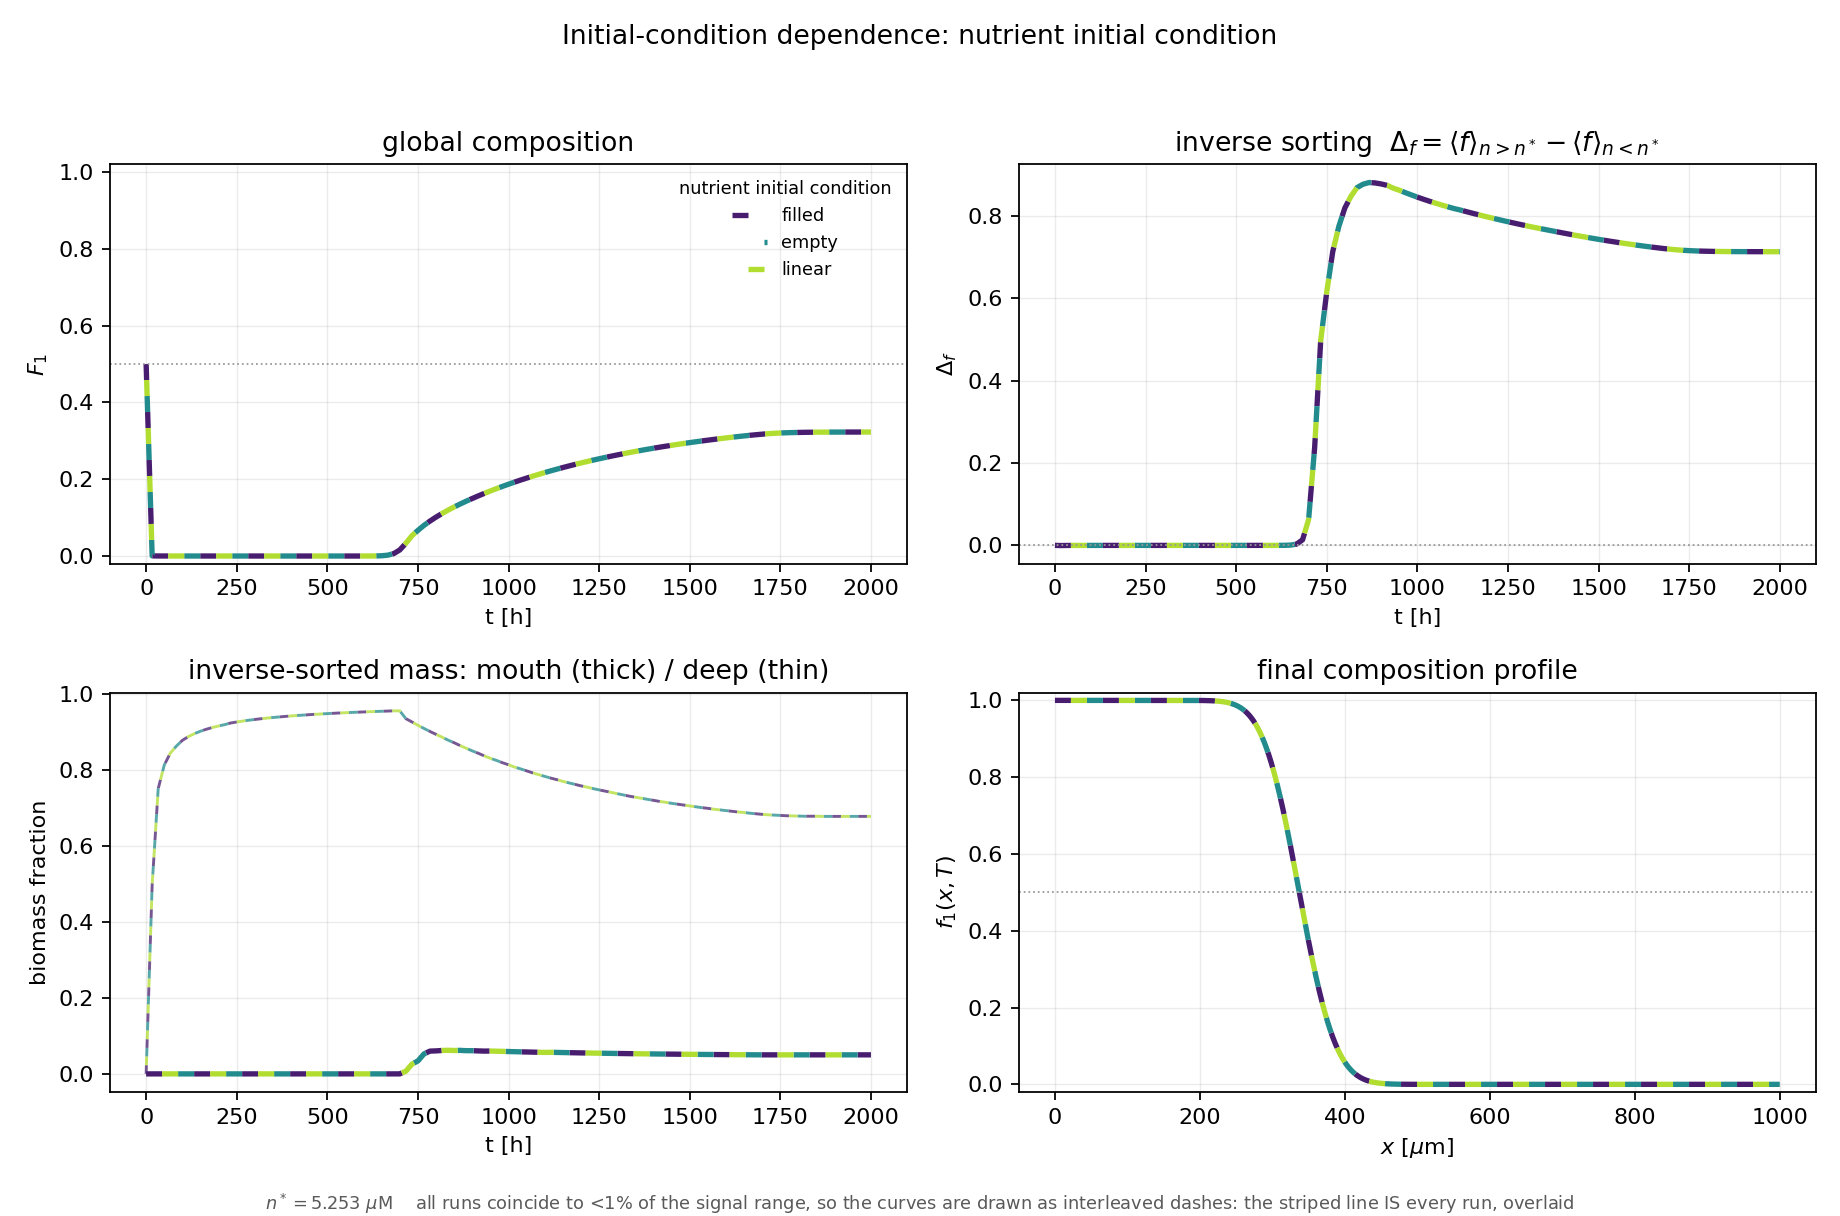
\includegraphics[width=\textwidth]{ic_nutrient_jam2}
		\caption{Jammed}
		\label{fig:jamic}
	\end{subfigure}
	\caption{Differing nutrient initial conditions (A) effect on global strain fraction $F1$, (B) how inverse sorting changes, (C) Split on mouth vs deep inverse sorting, (D) final profile at $T=2000h$.}
	\label{fig:nutrientic}
\end{figure}
\FloatBarrier
\paragraph{Differing cavity lengths and heterozygosity}
\label{sec:heterozygosity}
As a measure of spatial heterogeneity we use Wright and Nei's F-statistics \cite{Nei}. Their two allele solution for the coefficient of gene differentiation $F_{ST}$ can be directly transferred to our system. We use biomass as the subpopulation weight $w_i$.
\begin{equation}
	x_{i1}=f_i=\frac{\rho_{1,i}}{\rho_i},
	\qquad
	x_{i2}=1-f_i,
	\qquad
	w_i=\frac{\rho_i}{\sum_j \rho_j},
	\qquad
	\sum_i w_i=1 .
	\label{eq:fst-setup}
\end{equation}
which gives us
\begin{equation}
	F_{ST}=\frac{\mathrm{Var}_\rho(f)}{\bar f\,(1-\bar f)}
	\label{eq:fst-GST}
\end{equation}
with
\begin{equation}
	\bar f=\frac{\int_0^L \rho f\,dx}{\int_0^L \rho\,dx},
	\qquad
	\mathrm{Var}_\rho(f)=\frac{\int_0^L \rho\,(f-\bar f)^{2}\,dx}
	{\int_0^L \rho\,dx}.
	\label{eq:fst-continuum}
\end{equation}
So $F_{ST}$ is bounded between 0 (completely homogeneous) and 1 (entirely heterogeneous).
\begin{equation}
	0\le F_{ST}\le 1,
	\qquad
	F_{ST}=0 \iff \partial_x f\equiv 0,
	\qquad
	F_{ST}=1 \iff f\in\{0,1\}\ \text{a.e. on}\ \{\rho>0\}.
	\label{eq:fst-bounds}
\end{equation}
\begin{figure}
	\centering
	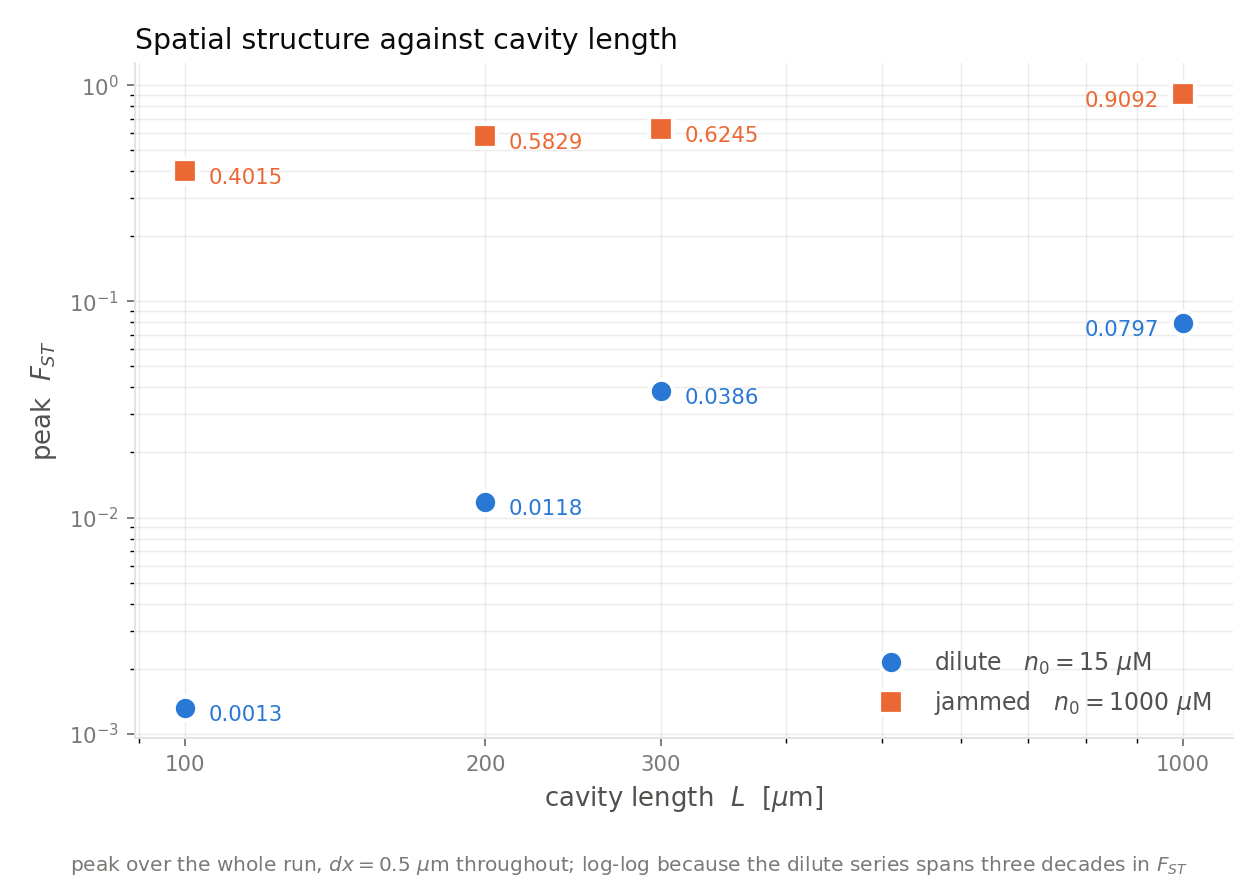
\includegraphics[width=0.6\linewidth]{fst_peak_vs_L}
	\caption{Peak spatial heterogeneity $F_{ST}$ over cavity length in the dilute (blue) and jammed (orange) regime}
	\label{fig:fstpeakvsl}
\end{figure}
\FloatBarrier
	\section{Numerical implementation and algorithms}
	\subsection{Solver}
	Even though the collective diffusion is supposed to pin $\rho$ near $\rho_{\mathrm{jam}}$ at very high nutrient supply $n_0$ it can fail to do so, resulting in a packing fraction above 1. However this would be unphysical, since biomass cannot occupy more than $100\%$ of the given space. As such we need to penalize growth above a certain threshold and disable it completely at $\rho=1$. Simply clipping the density does not work since growth would still be active, resulting in nonsense. To implement this we implement the growth factor $q$:
	\begin{equation}
		q(\rho)=\begin{cases}
			1, & \rho\le\rho_c,\\[2pt]
			\dfrac{\rho_{\mathrm max}-\rho}{\rho_{\mathrm max}-\rho_c}, & \rho_c<\rho<\rho_{\mathrm max},\\[6pt]
			0,&\rho\ge\rho_{\mathrm max},
		\end{cases}
		\qquad \rho_c=0.95,\ \rho_{\mathrm max}=1 .
		\label{eq:q}
	\end{equation}
	The factor $0.95$ was arbitrarily chosen by trial and error, it was found to still give sensible results even at extremely high $n_0$, bounding $0\le \rho \le 1$ over the tested range. It was tested up to $n_0=10^6 \mathrm{\mu M}$, in the main simulations used in this thesis the growth factor was never activated and was $q=1$ throughout all runs, so it had no influence. For significantly higher $n_0$ it is absolutely necessary, without $q$ at $n_0=10^6 \mathrm{\mu M}$ run would result in $\rho \approx 2$ \ref{sec:factor}, which we would want to avoid in the implementation even if we do not consider such a large food source. The solver is first order split, with the reaction–nutrient coupling and
	the jammed collective diffusion being solved implicitly using a damped Newton iteration with an analytic Jacobian. The CFL sub-cycling keeps the strain partition positive and the M-matrix structure of the label solve confines $f$ to $[0,1]$. \cite{Leveque} It uses a limiter (see \cref{convergence}).
	\subsection{Kernel decomposition}
	In the finite volume discretization, the neutral update over one time step has
	the matrix form
	\begin{equation}
		h_i^{m+1}=\sum_j P_{ij}^{m} h_j^{m}.
		\label{eq:discrete-neutral-update}
	\end{equation}
	Preservation of constants gives
	\begin{equation}
		\sum_j P_{ij}^{m}=1,
		\label{eq:discrete-row-sum}
	\end{equation}
	and positivity preservation gives
	\begin{equation}
		P_{ij}^{m}\ge 0 .
		\label{eq:discrete-positivity}
	\end{equation}
	So each row of \(P^m\) is the discrete ancestry distribution for the final
	cell \(i\).
	\paragraph{Discrete finite volume ancestry theorem}
Let \(h^m\in\R^{N_x}\) be the cell centered dominance vector before reaction at step \(m\)
and \(h^{r,m}\) the dominance vector after the local reaction but before neutral transport.
\(P_m\in\R^{N_x\times N_x}\) is the neutral transport matrix. Since \(P_m\one=\one\)
	\begin{equation}
		h^{m+1}=P_m h^{r,m}.
		\label{eq:discrete-transport}
	\end{equation}
	Define the nonlinear selection increment
	\begin{equation}
		\Delta h_{\rm sel}^m=h^{r,m}-h^m.
		\label{eq:delta-h-sel}
	\end{equation}
	Then \cref{eq:discrete-transport} becomes
	\begin{equation}
		h^{m+1}=P_mh^m+P_m\Delta h_{\rm sel}^m.
		\label{eq:discrete-recursion}
	\end{equation}
	Define the product
	\begin{equation}
		K^{a\to b}=P_{b-1}P_{b-2}\cdots P_a,
		\qquad 0\leq a<b\leq N_t,
		\label{eq:K-product}
	\end{equation}
	with \(K^{b\to b}=\Id\). Repeated substitution of \cref{eq:discrete-recursion} gives
	\begin{align}
		h^1 &=P_0h^0+P_0\Delta h_{\rm sel}^0,\nonumber\\
		h^2 &=P_1P_0h^0+P_1P_0\Delta h_{\rm sel}^0+P_1\Delta h_{\rm sel}^1,\nonumber\\
		h^3 &=P_2P_1P_0h^0+P_2P_1P_0\Delta h_{\rm sel}^0+P_2P_1\Delta h_{\rm sel}^1+P_2\Delta h_{\rm sel}^2,
	\end{align}
		For the finite volume update \(h^{m+1}=P_m(h^m+\Delta h_{\rm sel}^m)\), the final state is
		\begin{equation}
			{
				h^N=K^{0\to N}h^0+
				\sum_{m=0}^{N-1}K^{m+1\to N}P_m\Delta h_{\rm sel}^m.
			}
			\label{eq:discrete-exact}
		\end{equation}
	because of the inductive sequence: For \(N=1\), \cref{eq:discrete-exact} is \cref{eq:discrete-recursion}. Assume it holds at step \(N\). Then
		\begin{align}
			h^{N+1}
			&=P_Nh^N+P_N\Delta h_{\rm sel}^N\nonumber\\
			&=P_NK^{0\to N}h^0+
			\sum_{m=0}^{N-1}P_NK^{m+1\to N}P_m\Delta h_{\rm sel}^m
			+P_N\Delta h_{\rm sel}^N\nonumber\\
			&=K^{0\to N+1}h^0+
			\sum_{m=0}^{N-1}K^{m+1\to N+1}P_m\Delta h_{\rm sel}^m
			+K^{N+1\to N+1}P_N\Delta h_{\rm sel}^N\nonumber\\
			&=K^{0\to N+1}h^0+
			\sum_{m=0}^{N}K^{m+1\to N+1}P_m\Delta h_{\rm sel}^m.
		\end{align}
		So the identity holds for all \(N\).\\
		\\
	\paragraph{Evaluating the kernel}
Write \(w^m\) for the row of \(K^{m\to N}\) for a target cell \(i\) and unit vector \(e_i\)
\begin{equation}
	w^{N}=e_{i},
	\qquad
	w^{m}=P_m^{\mathsf T}\,w^{m+1}
	\label{eq:adjoint-recursion}
\end{equation}
turns \cref{eq:discrete-exact} into
\begin{equation}
	h^N_i=\bigl\langle w^{0},\,h^{0}\bigr\rangle
	+\sum_{m=0}^{N-1}\bigl\langle w^{m},\,\Delta h_{\rm sel}^m\bigr\rangle ,
	\label{eq:adjoint-pairing}
\end{equation}
at \(O(N_x)\) per step for one target per sweep. The h profile is solved directly as the adjoint of the discrete transport and the heatmaps for the kernel use a van Leer adjoint with a targeted FCT limier. \(\sum_i w^m_i=\sum_i w^{m+1}_i\) holds because the forward operator preserves constants \cref{eq:discrete-row-sum}. All kernel runs reported here use \(\Delta x=0.5\,\mathrm{\mu m}\) so \(N_x=2000\) and
are matrix free, \eqref{eq:adjoint-recursion} is iterated.
	\subsection{Convergence}
	\label{convergence}
	With our discretization used, convergence is sufficient for every value and regime except the jammed $F_1$ solution. However to see the value $F_1$ settles towards requires a very long run time if the population is jammed. We used $dx=0.5 \mathrm{\mu m}$, which already takes a long time to compute for the run to finish. Finer mesh refinement would take even longer, $dx=0.25\mathrm{\mu m}$ would require a significantly longer runtime, which also is not converged. If we would actually want an error below $1\%$, a single full run of the jammed simulation could take days or weeks, which is far from a reasonable computing time. General dynamics and observed effects seem to not be affected by mesh refinement, solely the actual strain fraction. So the qualitative picture stands, while reported strain fraction values in a jammed population have a $15.11 \%$ error, which is very large. These are the values for a $\rho_{\mathrm{seed}}=10^{-6}$ and without the limiter the main runs used (see below).\\
	\\
	The values that were actual measured compared to the extrapolated limit in the convergence test all have large errors:
	$$
	\begin{aligned}
		dx = 1 &: \quad +0.047057 \quad (+30.2\%) \\
		dx = 0.5 &: \quad +0.023572 \quad (+15.1\%) \\
		dx = 0.25 &: \quad +0.011786 \quad (+7.6\%)
	\end{aligned}
	$$
	This was run with $\rho_{\mathrm{seed}}=10^{-6}$. So even switching to e.g. $dx=0.25$ does not solve the issue, while massively increasing computing time. So with a coarser $dx$ the difference between measured $F_1$ values is larger, giving strain 1 more time establish itself before the composition freezes once the entire cavity is fully jammed. Leading to an earlier development of the high affinity specialist and a larger share of it later on once the composition freezes. A dilute cavity does not have that problem, because diffusion does not differ much in value across the run. The extrapolation is built from the $dx=0.25$ and $dx=0.5$ runs. This test was run with a final time of $T=1000h$, which is before the composition freezes at $t\approx 1750h$. Comparing two runs that have both frozen gives $F_1=0.3824$ at $dx=2\mathrm{\mu m}$ against $0.3186$ at $dx=0.5\mathrm{\mu m}$, so a difference of $20\%$. The time at which the composition freezes was measured to be consistent between tested $dx$, however the time at which strain 1 starts its recovery is not. Coarsening the grid moves the onset of this event earlier in time, the dip happens at $t=367h$ with $dx=2$ instead of $500h$ at $dx=0.5$. So the high affinity strain is given more time to built itself with a coarser mesh, resulting in a higher share of it in the final composition.

	\begin{table}[ht]
		\centering
		\caption{Discretization error at the values the unlimited runs used $dx=0.5\ \mu$m, $dt=0.05$ h.
			Each parameter was halved and doubled with the other fixed, $p$ is the
			measured order from the two successive differences and the limit is Richardson
			extrapolation $p=1$ using the two finest runs.The Error is the value relative to this limit.}
		\label{tab:conv-operating}
		\small
		\setlength{\tabcolsep}{5pt}
		\begin{tabular}{@{}lrrrrrrr@{}}
			\toprule
			& & \multicolumn{3}{c}{grid, $\Delta x = 1,\ 0.5,\ 0.25\ \mu$m}
			& \multicolumn{3}{c}{time step, $\Delta t = 0.1,\ 0.05,\ 0.025$ h}\\
			\cmidrule(lr){3-5}\cmidrule(lr){6-8}
			metric & value & $p$ & limit & error & $p$ & limit & error\\
			\midrule
			\multicolumn{8}{@{}l}{jammed reference: $n_0=1000\ \mu$M, $T=1000$ h}\\
			\addlinespace[1pt]
			$F_1$ & 0.179587 & 0.99 & 0.156016 & $+15.11$\% & --- & --- & $<0.112$\%\\
			$\rho_{\rm peak}$ & 0.657251 & 0.74 & 0.657414 & $-0.025$\% & --- & --- & $<0.001$\%\\
			$x_{n^*}$ & 69.7010 & 1.14 & 70.1747 & $-0.675$\% & 1.08 & 69.7488 & $-0.069$\%\\
			\addlinespace[3pt]
			\multicolumn{8}{@{}l}{dilute reference: $n_0=15\ \mu$M, $T=500$ h}\\
			\addlinespace[1pt]
			$F_1$ & 0.905888 & 0.81 & 0.905922 & $-0.0038$\% & 0.95 & 0.905247 & $+0.071$\%\\
			$\rho_{\rm peak}$ & 0.012225 & --- & --- & $<0.001$\% & 1.07 & 0.012222 & $+0.023$\%\\
			$x_{n^*}$ & 32.9791 & 2.05 & 32.9807 & $-0.0050$\% & 1.00 & 33.0626 & $-0.253$\%\\
			\bottomrule
		\end{tabular}
	\end{table}
\FloatBarrier
This happens because our solver transports labels between grid cells with width $dx$, so it needs the fraction at the face between them. But values are only stored at grid centers, so it is guessed by taking the value of the grid cell the flow is coming from. This value however also sits half a grid cell upstream of the face, so every face is fed from a wrong place. Repeating this over and over again results in an error scaling with $\tfrac12\Delta x$. So a larger $dx$ means a larger value offset and such a bigger error. In a jammed cavity the self diffusion collapses to a tiny value much smaller than the error which results in this error taking over. Meaning that this error is essentially acting as label diffusion, diffusing more of strain 1 into the growth band and thus more overestimating its prominence.
The strain label is advected by donor-cell upwinding. On a uniform grid with $u>0$ and an
advection sub step $h$, the update at grid cell $i$ is
\begin{equation}
	f_i^{m+1} = f_i^m - \nu\left(f_i^m - f_{i-1}^m\right),
	\qquad \nu = \frac{u\,h}{\Delta x},
	\label{eq:upwind}
\end{equation}
where $\nu$ is the Courant number \cite{Leveque}. Taylor expanding both sides about $(x_i,t_m)$
\begin{align}
	f_i^{m+1} &= f + h\,\partial_t f + \tfrac{1}{2}h^2\,\partial_{tt} f + \mathcal{O}(h^3),
	\label{eq:tayt}\\
	f_{i-1}^m &= f - \Delta x\,\partial_x f + \tfrac{1}{2}\Delta x^2\,\partial_{xx} f
	+ \mathcal{O}(\Delta x^3),
	\label{eq:tayx}
\end{align}
\begin{equation}
	f_i^m - \nu\left(f_i^m - f_{i-1}^m\right)
	= f - u h\,\partial_x f + \frac{u h \Delta x}{2}\,\partial_{xx} f
	+ \mathcal{O}(\Delta x^3).
	\label{eq:rhs}
\end{equation}
Equating \eqref{eq:tayt} and \eqref{eq:rhs} and dividing by $h$,
\begin{equation}
	\partial_t f + \frac{h}{2}\,\partial_{tt} f
	= -u\,\partial_x f + \frac{u\,\Delta x}{2}\,\partial_{xx} f
	+ \mathcal{O}(\Delta x^2, h^2).
	\label{eq:mid}
\end{equation}
To leading order the scheme obeys $\partial_t f = -u\,\partial_x f$, so
\begin{equation}
	\partial_{tt} f = -u\,\partial_x\!\left(\partial_t f\right) = u^2\,\partial_{xx} f,
	\label{eq:ftt}
\end{equation}
and substituting \eqref{eq:ftt} into \eqref{eq:mid} gives
\begin{align}
	\partial_t f + u\,\partial_x f
	&= \frac{u\,\Delta x}{2}\,\partial_{xx} f - \frac{h\,u^2}{2}\,\partial_{xx} f \nonumber\\
	&= \frac{u\,\Delta x}{2}\left(1 - \frac{u h}{\Delta x}\right)\partial_{xx} f
	= \underbrace{\frac{u\,\Delta x}{2}\left(1-\nu\right)}_{\textstyle D_{\mathrm{num}}}\,
	\partial_{xx} f .
	\label{eq:modified}
\end{align}
The same expansion for $u<0$ gives
\begin{equation}
	{\;D_{\mathrm{num}} = \tfrac{1}{2}\,\lvert u\rvert\,\Delta x\,
		\bigl(1-\lvert\nu\rvert\bigr).\;}
	\label{eq:dnum}
\end{equation}
So increasing $dx$ directly feeds into the numerical "diffusion", making the final $f$ value untrustworthy.
A way to fix this is using Flux corrected transport (FCT) and introducing a Van Leer flux limiter
$f_{\mathrm{face}} = f_{\mathrm{donor}} + \frac{1}{2}\,\mathrm{limited}(a,b)$, which cancels the half grid cell offset. Near a sharp front this correction switches off to avoid an overshoot outside of the $[0,1]$ bound for $f$. Using it all the time would also make the profile oscillate and not using it results in large errors, so this switch is a sensible solution.
\begin{figure}
	\centering
	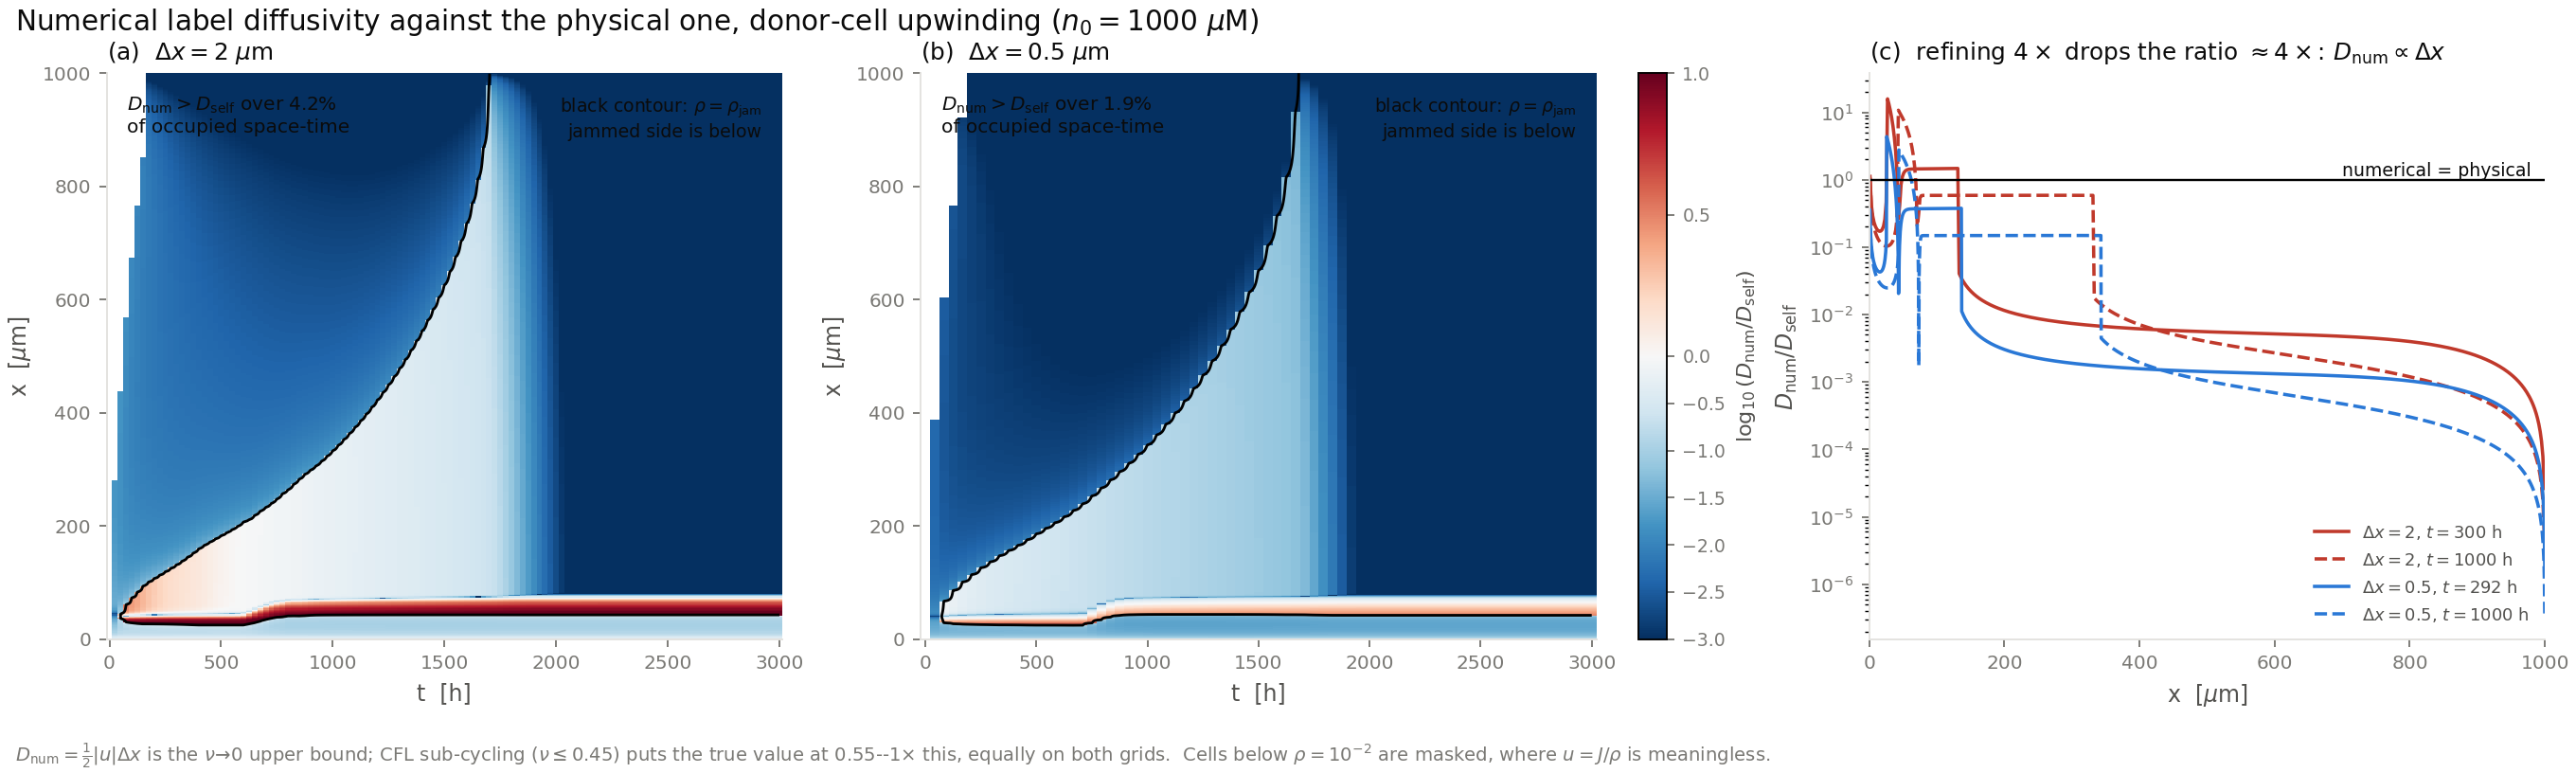
\includegraphics[width=0.7\linewidth]{dnum_over_dself}
	\caption{Comparison of the effect of numerical diffusion against self diffusion}
	\label{fig:dnumoverdself}
\end{figure}
\FloatBarrier
Another issue is that $\rho_{\mathrm{seed}}=10^{-6}$ would be far below one single cell \cref{sec:extinction}, so main runs reported in results used $\rho_{\mathrm{seed}}=10^{-4}$. The final composition in the main simulation with $dx=0.5 \mathrm{\mu m}$ have an error of $1.77\%$ (\ref{fig:gridconvergencet2000}, panel (a)), which is admissible. The composition is frozen at $T=2000 \mathrm{h}$, but ever so slightly drifts afterwards, it was chosen over the main jammed runtime $T=6000\mathrm{h}$ since $dx=0.25 \mathrm{\mu m}$ has a very large runtime. Mesh refinement converges first order \ref{fig:gridconvergencet2000} (panel (b)), to obtain the limit we assume the discretization error is dominated by one power of $dx$. So $F(dx,T)=F_{\mathrm{limit}}+K dx^{n}+O(dx^{n+1})$ \cite{sauer}, since we used $dx=2,1,0.5,0.25$ our refinement ratio is $r=2$. As such we get the differences $d_1=F(1,T)-F(0.5,T)=K0.5^{n}(2^{n}-1)$ and $d_2=F(0.5,T)-F(0.25,T)=K0.25^{n}(2^{n}-1)$, so $\frac{d_1}{d_2}=2^{n}$. Our measured values are $F(dx=1,T=2000h)=0.3279060, F(dx=0.5,T=2000h)=0.3229142, F(dx=0.25,T=2000h)=0.3202739$, so $d_1 = 0.0049918$, $d_2= 0.0026403$, $\frac{d_1}{d_2}= 2^n = 1.89062$, $n = 0.91886$. We get the limit value by Richardson extrapolation $F_{\mathrm{limit}}=F(0.25,T)-\frac{d_2}{2^n-1}=0.3173093$. The coarse $dx=2$ value was deliberately excluded from the extrapolation due to its large error. The profile limit was obtained by reusing $n$ and interpolation.
\begin{figure}
	\centering
	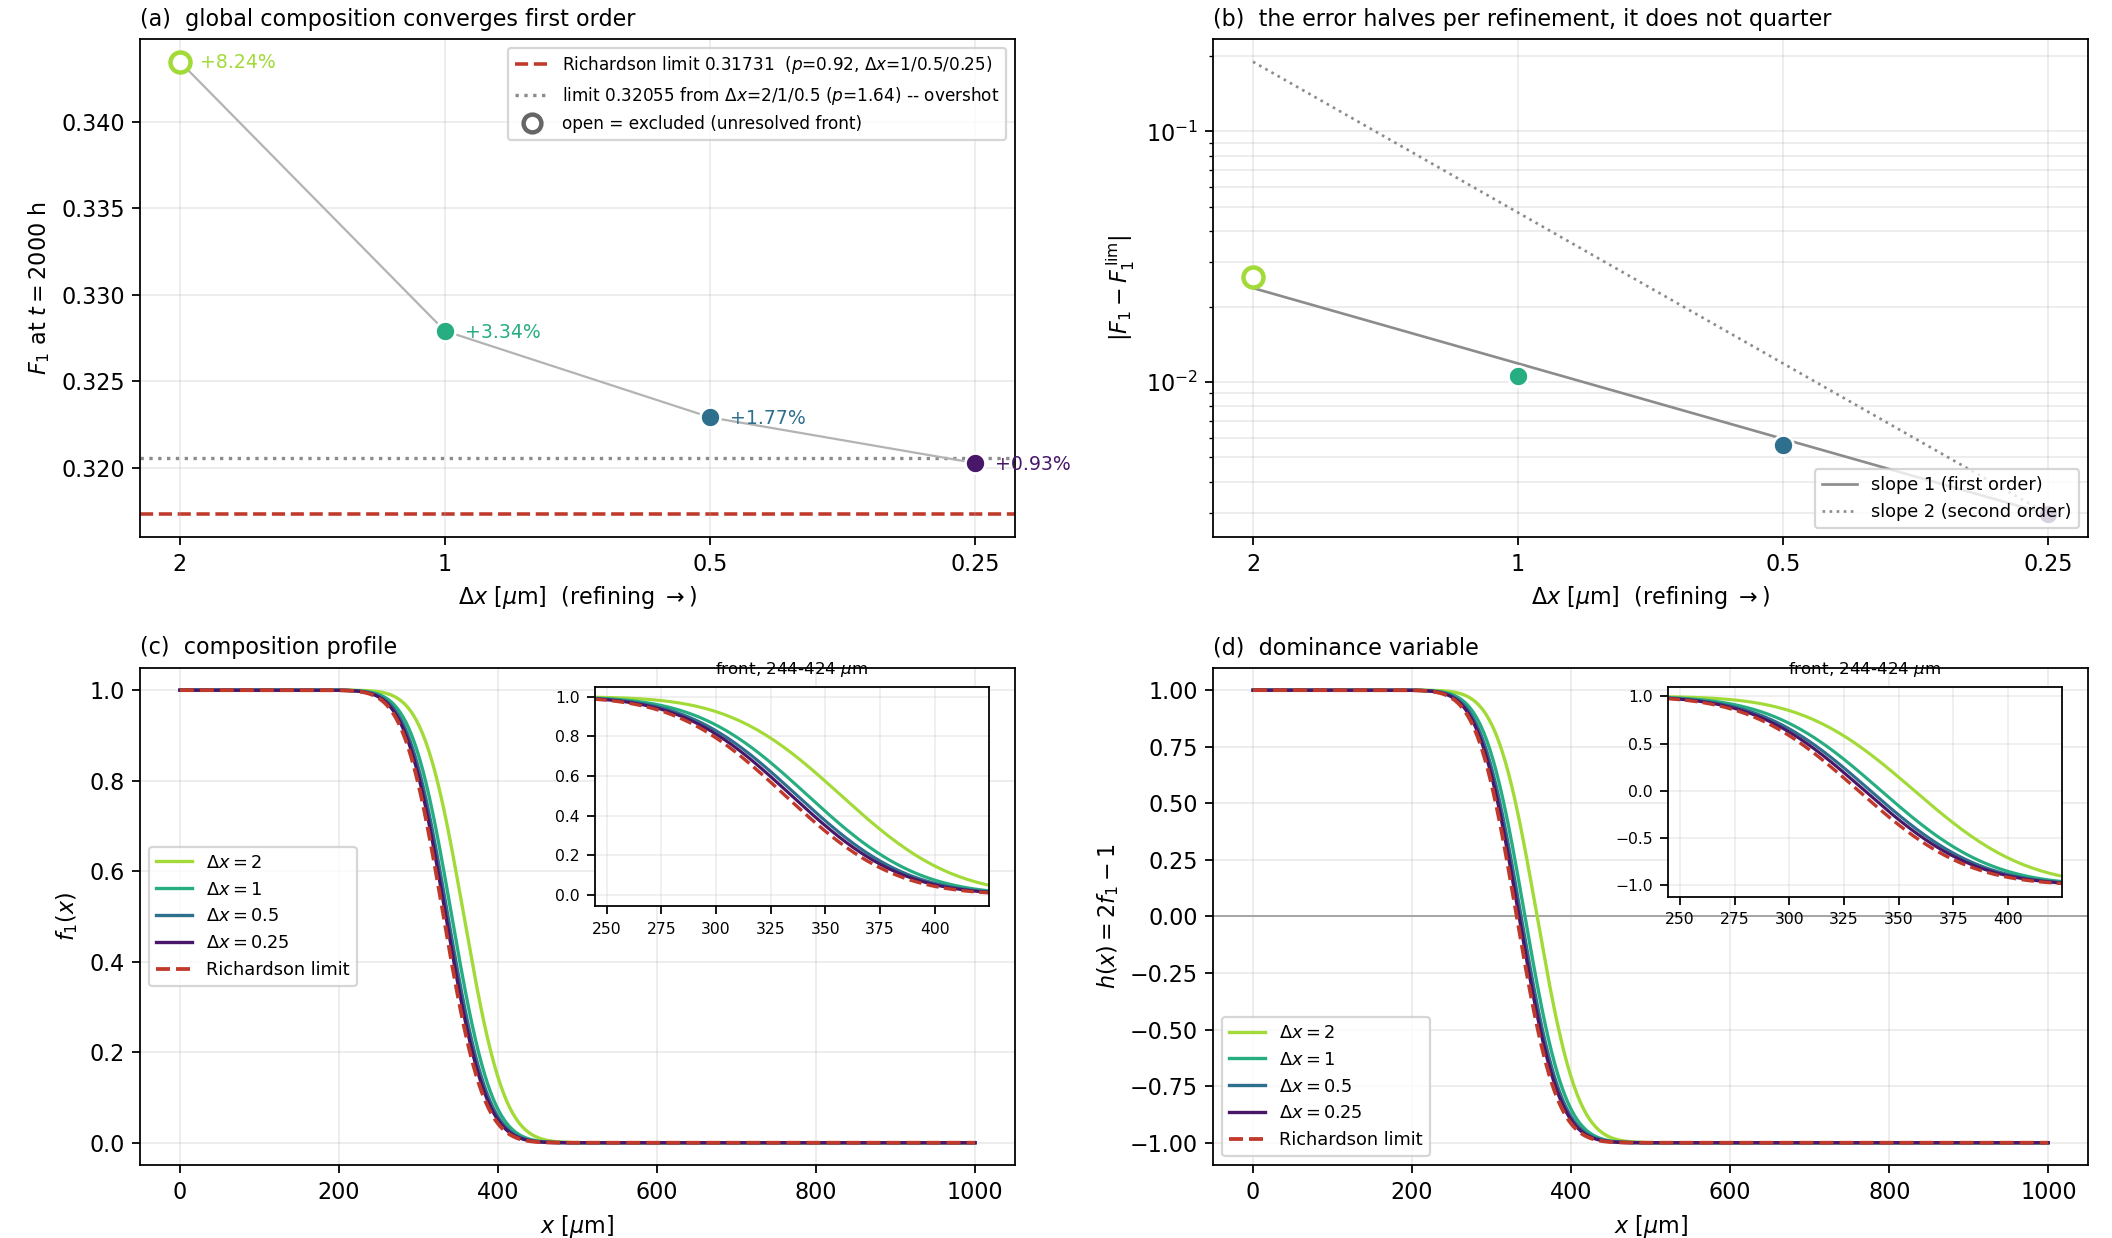
\includegraphics[width=\linewidth]{grid_convergence_T2000}
	\caption{Grid convergence of the jammed run, $n_0=1000 \mathrm{\mu M}$, $L=1000\mathrm{\mu m}$, $\rho_{\mathrm{seed}}=10^{-4}$, $T=2000\mathrm{h}$, van Leer limiter and Richardson limit, (a) Global composition at final time, (b) Errors relative to the limit, (c) Final profile $f_1$ over position, (d) Dominance variable $h$ over position at final time-}
	\label{fig:gridconvergencet2000}
\end{figure}
\FloatBarrier
The kernel implementation shows a trend of convergence with decreasing $dx$ in the jammed case, where the theory run has a significant error near the opening due to the same numerical diffusion problem (\cref{fig:adjointconvergenceoverlay}). The introduction of the same Van Leer limiter to fix the numerical diffusion would lead to the kernel possibly having negative entries and as such it would lose its interpretation as an ancestral probability distribution showing the mean trajectory.
\begin{figure}
	\centering
	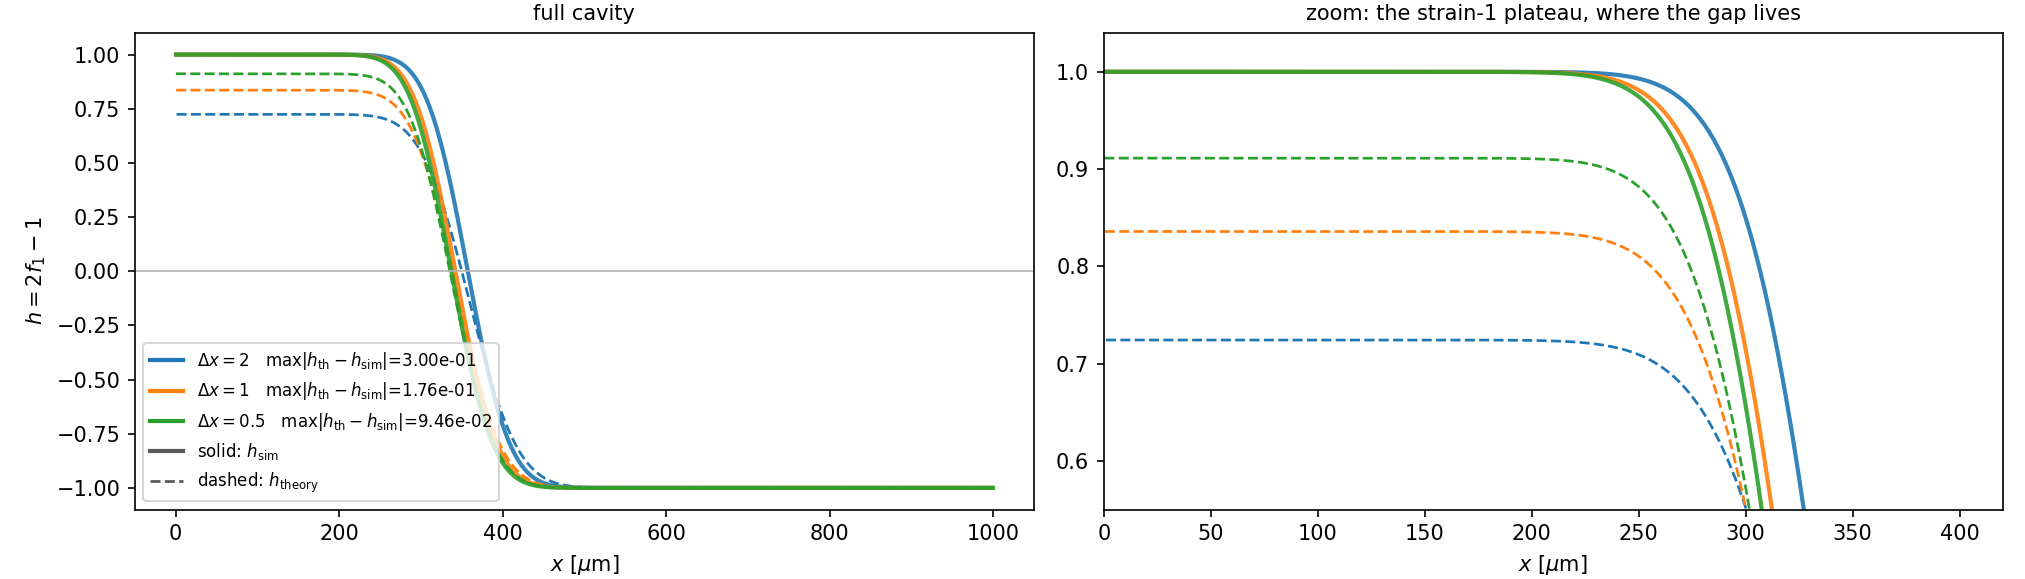
\includegraphics[width=\linewidth]{adjoint_convergence_overlay}
	\caption{Dominance variable $h$ over position at final time $T=2000h$ in the jammed case $n_0=1000 \mathrm{\mu M}$. Theory and numerical values for $dx=2,1,0.5 \mathrm{\mu m}$}
	\label{fig:adjointconvergenceoverlay}
\end{figure}
\FloatBarrier
\subsection{Extinction}
\label{sec:extinction}
Our model is a continuum and as such there is no definition of a cell directly implemented, which means we dont have a direct way of quantifying whether or not a strain had gone extinct or not. To tell if there is enough biomass to form at least one cell we assume our cavity to be a squashed in microfluidic panflute. The experimental device has the dimensions $L \times 20 \mathrm{\mu m} \times 50 \mathrm{\mu m}$ \cite{Karita} and an average E. coli cell has a volume of $0.6-0.7 \mathrm{\mu m}^3$ \cite{volume}. So the amount of cells in our cavity is $N=\frac{MA}{V_{\mathrm{cell}}}$ with $A=50\times20 \mathrm{\mu m}^2=1000\mathrm{\mu m}^2$, $M=\int_{0}^{L}\rho_{i}(x)\,dx$ for strain $i$ and $V_{\mathrm{cell}}=0.65\mathrm{\mu m}^3$. So the extinction floor for each strain is $M_{i}=0.00065 \mathrm{\mu m}$, meaning there is enough biomass in the cavity left to form one cell of strain $i=1,2$. If a strain dips below this value it is considered extinct and the other strain respectively is crowned the victor, successfully excluding its competitor.
	\paragraph{Use of Large Language Models (LLMs)}
	The LLM Claude Code was used for programming in Python, numerical methods, preliminary data analysis of large data sets, GitHub, LaTeX formatting, review purposes and finding relevant literature.
	\chapter{Discussion}
	\section{Interpretation and relation to existing literature}
	A carious lesion is a dead end pore ranging from the micron to millimeter scale, with cells forming biofilm colonies consisting of Streptococcus and Lactobacillus \cite{lesion}. Dige et al. found that genetic diversity at the opening is larger and more heterogeneous than in the interior. Our mechanical analysis suggest that under nutrient limitation this could be due to an early time advantage of one strain that got advected inwards and stranded while the opening remains temporarily competitive around the $n^*$ front. For example a dilute cavity after 4 days carries this signature \ref{fig:hdil}. So in our interpretation the deep lesion composition would consist of which strain had the early time advantage and not who is more adapted to the local environment. The general conclusion of our analysis is that a composition snapshot at a point in time is not indicative of the individual strain properties as they can largely sort against their advantage.\\
	\\
	Strains occupying regions where they are disfavored has previously been described in the form of gene surfing, caused by a stochastic drift \cite{gene} \cite{lifeexp} \cite{stepping}. As a colony expands its habitat, the front of the colonization is sparse with decaying heterozygosity. Meaning that the stochastic drift carries the lesser fit strain into the habitat, making it occupy disfavored regions. Our model is deterministic, meaning that it only holds validity in the bulk as in small populations stochastic effects dominate. As such it can be seen as the deterministic counterpart to gene surfing.
	\section{Limitations}
	The central inverse sorting criterion deals in absolutes, meaning that biomass is only classified as inverse if the historical selection the cells went through disagrees with the current advantage \eqref{eq:exposure-criterion2}. However if we would for example consider a strain fraction with a monotonically decreasing profile, but with all f values being dominates by one strain, e.g. $f(x,t)\le0.5$ for a fixed point in time. Then an inverse sorted opening cannot exist, since it favors and is dominated by the glutton, however there would still be a bigger share of the high affinity strain in sections where it is disfavored (opening) compared to regions where it has the advantage (interior and deep). So in relative terms the profile or trend is still inverse, but the criterion would characterize the opening as normally sorted since the the correct strain wins. Inverse sorted biomass can still have an increasing profile in the section, as for example in a dilute cavity \ref{fig:hdil}, so a non-monotone fraction function can still be inverse sorted in its increasing region, so reducing the criterion to a decreasing profile is also not valid. Two separate categorizations of the existing "absolute" inverse sorting and "relative" inverse sorting could be sensible, since each have their own drawbacks.\\
	\\
	A large simplification was made in this model, which is the omission of cell death. In confined cavities cell death was not found within the span of a couple days \cite{Karita}, which fits the timescale of our dilute analysis. However these cells were not starved, nutrient was abundant, the opposite of our model. But again it is totally reasonable to assume that even starved cells can survive for a couple days without food. The timescale of the jammed cavity is where it comes back to bite us, since in a long cavity to observe all effects of the dynamic range you would need starved cells to survive a much longer time. For example to observe the freezing of the composition, cells would need to survive over 2 months without food \ref{fig:runjam}, which is much less realistic. Even if the cells were to survive that long, starved cells are known to shrink, which could unjam the cavity and thus destroy the frozen composition and coexistence result \cite{starved}.\\
	\\
	After the initial nutrient rich expansion phase the interior and deep end of the cavity have nutrient concentrations below the noise floor (\cref{fig:rundilute}, \cref{fig:runjam}). This however means that apart from the near opening region, where biomass is produced (\cref{sec:prod}), the cavity is a selection free zone. If the nutrient concentration is merely numerical noise, no one is being selected and thus the high affinity strain does not have an advantage there anymore. As such the glutton is not inverse sorted at the deep end since no one is favored if no one can grow at all. If we take the nutrient concentration output of the simulation instead of setting the noise floor to zero, the high affinity strain does have a slight advantage. However the $n(x,t)$, which should have an exponential profile throughout, becomes linear under the noise floor, so the output cannot be trusted for extremely low concentrations which is why we label it as numerical noise. However the advantage $\sgn(s)$ depends solely on which side of the crossover at $n^*=5.25 \mathrm{\mu M}$ the concentration sits, so whatever the exact profile in the numerical noise regime is, we know it to be well below $n^*$. So the advantage survives, even with untrustworthy nutrient concentrations. The high affinity strains advantage grows as the nutrient concentration falls, $\frac{g_1}{g_2} \to \frac{\mu_1 K_2}{\mu_2 K_1} = 20.19$ as $n \to 0$. Even if the entire deep end and interior would contain an accumulated concentration below one glucose molecule, a neutral zone $s \to 0$ producing a strong prominence of the glutton strain is not normal sorting and cannot be explained by the local environment. As such we still call it inverse sorted, as the $\sgn(s)$ advantage is still there and the composition can only be inherited, even if the region cannot produce significant growth for either strain.\\
	\\
	The seed has a low cell count of 7 and the high affinity strain is about 20 cells at its jammed bottleneck (\cref{fig:runjam}, \cref{sec:extinction}). But a continuum formulation is a bulk approximation, at such low cell counts stochastic effects would dominate. This would turn the strains recovery into a chance event since in a stochastic system it would not be guaranteed that there are any high affinity cells in the growth band (\cref{sec:prod}).
	\section{Outlook}
	An interesting consideration would be the inclusion of chemotaxis as the washout opening would become a death trap for cells chasing the nutrient gradient too greedily. Chemotaxis being the source of a cell swimming towards their death has previously been observed by chasing the toxic antibiotic gradient, actively committing suicide \cite{suicide}. When the glutton chases the nutrient gradient more strongly than the high affinity strain, this could counteract the expansion phase where it colonizes the interior and deep end. It would be decided by comparing advection with chemotactic effects, a jammed cavity could possibly even return to being normally sorted if the glutton is pinned towards the opening. Similar to how cell death or shrinkage could also slowly get rid of the glutton graveyard at the deep end. Another important mechanism in bacterial colonization is cross feeding \cite{cross}, where a strain excretes a chemical after consuming nutrients, which can be consumed gain, by e.g. the other. This could also heavily alter dynamics, since if e.g. the high affinity strain is the sole consumer of the excrete it can make up the growth disadvantage in the earlier stages by having a higher nutrient availability. Even if both strains eat each others excretes, because the glutton has a much higher consumption initially, this would give the high affinity strain more nutrients to consume and grow by, potentially leading to a stronger recovery. In our simulations the inside of the cavity quickly becomes devoid of nutrients and growth is exclusive to a small band near the opening. By recycling the interior can be supplied with excretes nutrients by the cells themselves, giving a chance to the high affinity strain to actually realize their local growth advantage there. 
	
	\chapter{Conclusion}
	We investigated phase transitions under nutrient limitation, showing that it can lead to a continuous jamming transition, which was previously only known as abrupt in nutrient rich colonies \cite{Karita}. The establishment transition in opposition is always gradual, making it a continuous process. We derived and numerically validated the threshold length formula, directly relating cavity length and the nutrient exhaustion needed to reach it in steady state. Assuming an entirely jammed or dilute cavity allows significant simplifications on the system making it analytically solvable. Most notably we discovered the inverse sorting phenomenon, in which strains sort, at certain points in time even entirely, against their advantage. This effect is transient in dilute population, but the jammed regime can make it freeze over any reasonable timescale for real cells making it essentially permanent for the cells lifespan. The kernel decomposition was developed as a theoretical description of the problem, with the central theorem determining if the composition is inverse sorted at a certain point in time. This works by weighing biomass contributions of all past points in time, with the history being split in a reinforcing and opposing exposure. Meaning does the historical selection that contributed to this point agree with the current advantage or not. The PDE was solved analytically with the duhamel formula. Nutrient concentration and cavity length were both found to be positively correlated to spatial heterogeneity, making a long nutrient rich cavity almost entirely spatially diverse with strongly segregated strains and a short dilute cavity essentially well-mixed. 
	\printbibliography

	\appendix
	\chapter{Supplementary Notes}
	\section{Algebraic reduction of the sub-jamming collective diffusivity}
	\label{subsec:Dcol_derivation}
	\begin{equation}
		{
			D_{\rm col}(\rho)
			=
			D_0
			\frac{\mu(\Phi(\rho))\,dP(\Phi(\rho))}
			{\mu(0)\,dP(0)}
		}
		\qquad 0\le \rho<\rho_{\rm jam}.
	\end{equation}
	The Richardson-Zaki mobility and the Carnahan-Starling
	equation of state \cite{carnahan} \cite{zaki} \cite{Karita} \cite{slepukhin} are
	\begin{equation}
		\mu(\Phi)=\mu_0(1-\Phi)^{\eta},
		\qquad
		P(\Phi)=\frac{6}{\pi}\,\Phi\,A(\Phi),
		\qquad
		A(\Phi)=\frac{1+\Phi+\Phi^2-\Phi^3}{(1-\Phi)^3},
	\end{equation}
	write $N=1+\Phi+\Phi^2-\Phi^3$ and the first derivative $N'=1+2\Phi-3\Phi^2$
	\begin{align}
		\partial_\Phi A
		=\frac{N'(1-\Phi)^3+3N(1-\Phi)^2}{(1-\Phi)^6}
		=\frac{N'(1-\Phi)+3N}{(1-\Phi)^4}
		=\frac{4+4\Phi-2\Phi^2}{(1-\Phi)^4}
	\end{align}
	\begin{align}
		A+\Phi\,\partial_\Phi A
		=\frac{(1-2\Phi^3+\Phi^4)+(4\Phi+4\Phi^2-2\Phi^3)}{(1-\Phi)^4}
		=\frac{1+4\Phi+4\Phi^2-4\Phi^3+\Phi^4}{(1-\Phi)^4}
	\end{align}
	\begin{align}
		dP=\frac{6}{\pi}A+\frac{6\Phi}{\pi}\partial_\Phi A
		=\frac{6}{\pi}(A+\Phi\,\partial_\Phi A)
		=\frac{6}{\pi}\frac{1+4\Phi+4\Phi^2-4\Phi^3+\Phi^4}{(1-\Phi)^4}
	\end{align}
	with $dP(0)=\frac{6}{\pi}$ and $\mu(0)=\mu_0$.
	\begin{equation}
		\frac{\mu(\Phi)\,dP(\Phi)}{\mu(0)\,dP(0)}
		=
		\frac{\frac{6}{\pi}\mu_0(1-\Phi)^{\eta}}{\mu_0\frac{6}{\pi}}\frac{1+4\Phi+4\Phi^2-4\Phi^3+\Phi^4}{(1-\Phi)^4}
		=
		(1-\Phi)^{\eta-4}(1+4\Phi+4\Phi^2-4\Phi^3+\Phi^4)
	\end{equation}
	with $\Phi=\rho$ we get
	\begin{equation}
		{D_{\rm col}(\rho)
			=
			D_0(1-\rho)^{\eta-4}
			(1+4\rho+4\rho^2-4\rho^3+\rho^4),
			\qquad \rho\le\rho_{\rm jam}
		}
	\end{equation}

\section{Invariant}
\label{invariant}
Then
\begin{equation}
	\Psi(0)=0,
	\qquad
	\Psi_x=D_{\rm col}(\rho)\rho_x.
\end{equation}
and
\begin{equation}
	J_\rho=-\Psi_x.
\end{equation}
The steady state biomass equation becomes
\begin{equation}
	{
		\Psi_{xx}+g(n)\rho=0.
	}
	\label{eq:steady_pressure_new}
\end{equation}
\[
\Psi'(\rho)=D_{\rm col}(\rho)>0.
\]
for $\rho \in$ $[0,1]$. So $\Psi$ is strictly increasing on $[0,1]$, so it follows that it is one to one injective. Thus every value in the image $\Psi\bigl([0,1])$ has a unique preimage. And so it
has a well defined inverse on its image
\[
\Psi^{-1}:\Psi\bigl([0,1])\bigr)\to[0,1].
\]
$\Psi^{-1}(p)$ is the density
$\rho\in[0,1]$ satisfying
\[
\Psi(\rho)=p.
\]
This definition allows us to rewrite the coupled system into only one differential equations.
Using \eqref{eq:steady_pressure_new} and \eqref{eq:steady_n_new},
\begin{equation}
	\Psi_{xx}=-g(n)\rho,
	\qquad
	YD_n n_{xx}=g(n)\rho.
\end{equation}
Adding gives
\begin{equation}
	\Psi_{xx}+YD_n n_{xx}=0.
\end{equation}
so
\begin{equation}
	\frac{d}{dx}\left(\Psi_x+YD_n n_x\right)=0,
\end{equation}		
\begin{equation}
	\Psi_x+YD_n n_x=C.
\end{equation}
with $C$ being a constant. At the bottom: $J_\rho(L)=0$ gives $\Psi_x(L)=0$, and $n_x(L)=0$ by the
nutrient no-flux boundary condition.  Therefore $C=0$.
So with \eqref{eq:steady_rho_new}--\eqref{eq:steady_bcs_new} and
$0\le \rho\le 1$ and $n\ge0$ on $[0,L]$. We get
\begin{equation}
	{
		D_{\rm col}(\rho)\rho_x+YD_n n_x=0.
	}
	\label{eq:flux_invariant_new}
\end{equation}	
\begin{equation}
	{
		\Psi_x+YD_n n_x=0.
	}
	\label{eq:Psi_invariant_new}
\end{equation}
Integrating from $0$ to $x$:
\begin{equation}
	\Psi(\rho(x))-\Psi(\rho(0))
	=-YD_n\bigl(n(x)-n(0)\bigr).
\end{equation}
Using $\rho(0)=0$, $\Psi(0)=0$ and $n(0)=n_0$ gives
\begin{equation}
	{
		\Psi(\rho(x))=YD_n\bigl(n_0-n(x)\bigr).
	}
	\label{eq:integrated_invariant_zero_opening}
\end{equation}
\begin{equation}
	{
		\Psi(\rho(x))+YD_n n(x)=YD_n n_0.
	}
	\label{eq:level_set_zero_opening}
\end{equation}
The invariant holds to numerical precision with a residual of $3.4\times 10^{-16}$ \ref{fig:steadyclosures}. $\Psi$ is quickly rising at the opening of the cavity and since the flux is defined as $J_\rho=-\Psi_x$, this represents the washout opening.
\section{Spatial Profiles in the Dilute Regime}
\label{dilute_profiles_corrected}	
The integrated invariant gives
\begin{equation}
	n(p)=n_0-\frac{p}{YD_n}.
\end{equation}	
Let $n_*\in(0,n_0)$ be the prescribed nutrient threshold at the closed
end.  Then
\begin{equation}
	p_*=YD_n(n_0-n_*).
\end{equation}
The pressure flux satisfies
\begin{equation}
	q(p)=p_x
	=
	\sqrt{
		\frac{2}{D_0}
		\int_p^{p_*}
		g\!\left(n_0-\frac{s}{YD_n}\right)s\,ds
	}.
	\label{eq:q_dilute_full_profile}
\end{equation}
Therefore
\begin{equation}
	x(p)
	=
	\int_0^p
	\frac{du}
	{
		\sqrt{
			\frac{2}{D_0}
			\int_u^{p_*}
			g\!\left(n_0-\frac{s}{YD_n}\right)s\,ds
		}
	}.
	\label{eq:x_of_p_dilute_full}
\end{equation}
Equations \eqref{eq:x_of_p_dilute_full},
\[
n(p)=n_0-\frac{p}{YD_n},
\qquad
\rho(p)=\frac{p}{D_0},
\]
give the parametric dilute profiles for arbitrary Monod kinetics.\\	
Using nutrient concentration itself as the parameter
\[
p=YD_n(n_0-n).
\]
we get
\[
dp=-YD_n\,dn.
\]
For the inner integral set
\[
s=YD_n(n_0-m),
\qquad
ds=-YD_n\,dm.
\]
When $s=p$ we have $m=n$ and when $s=p_*$ we have $m=n_*$.
Therefore
\begin{align}
	\int_p^{p_*}
	s\,g\!\left(n_0-\frac{s}{YD_n}\right)\,ds
	&=
	\int_n^{n_*}
	YD_n(n_0-m)g(m)(-YD_n)\,dm \\
	&=
	(YD_n)^2
	\int_{n_*}^{n} g(m)(n_0-m)\,dm.
	\label{eq:inner_integral_n_variable}
\end{align}
So
\[
q(p(n))
=
YD_n
\sqrt{
	\frac{2}{D_0}
	\int_{n_*}^{n}g(m)(n_0-m)\,dm
}.
\]
Using $dp=-YD_n\,dn$ the factors $YD_n$ cancel in $dx=dp/q$. So
the position at which the nutrient has value $n$ is
\begin{equation}
	{
		x(n)
		=
		\int_n^{n_0}
		\frac{d\eta}
		{
			\sqrt{
				\frac{2}{D_0}
				\int_{n_*}^{\eta}
				g(m)(n_0-m)\,dm
			}
		}.
	}
	\label{eq:x_of_n_dilute_full}
\end{equation}
$\eta$ is the outer nutrient integration variable and $m$ is the
inner dummy variable.\\
The associated density profile
\begin{equation}
	{
		\rho(x(n))
		=
		\frac{YD_n}{D_0}(n_0-n).
	}
	\label{eq:rho_of_n_dilute_full}
\end{equation}
At the opening
\[
x=0,
\qquad
n=n_0,
\qquad
\rho=0.
\]
At the threshold point
\[
x=L_*,
\qquad
n=n_*,
\qquad
\rho(L_*)=
\frac{YD_n}{D_0}(n_0-n_*).
\]	
Under the additional low-nutrient approximation
\[
g(n)\approx kn,
\]
the inner integral in \eqref{eq:x_of_n_dilute_full} becomes
\begin{align}
	\int_{n_*}^{\eta} g(m)(n_0-m)\,dm
	&\approx
	\int_{n_*}^{\eta} k m(n_0-m)\,dm \\
	&=
	k\int_{n_*}^{\eta}(n_0m-m^2)\,dm \\
	&=
	k\left[
	\frac{n_0}{2}(\eta^2-n_*^2)
	-
	\frac{1}{3}(\eta^3-n_*^3)
	\right].
\end{align}
Therefore the low nutrient dilute profile is
\begin{equation}
	{
		x(n)
		=
		\int_n^{n_0}
		\frac{d\eta}
		{
			\sqrt{
				\frac{2k}{D_0}
				\left[
				\frac{n_0}{2}(\eta^2-n_*^2)
				-
				\frac{1}{3}(\eta^3-n_*^3)
				\right]
			}
		}.
	}
	\label{eq:x_of_n_dilute_linear}
\end{equation}
	\section{Exact depletion is mathematically an infinite length statement}
	\label{sec:n0}
	Assume by contradiction that $n(L)=0$. From the boundary condition we have
	$n_x(L)=0$, so the intial values at $x=L$ are
	\[
	n(L)=0,
	\qquad
	n_x(L)=0.
	\]
	Set
	\[
	y_1=n,
	\qquad
	y_2=n_x.
	\]
	Then the nutrient equation can be written as the first-order system
	\[
	y_1'=y_2,
	\qquad
	y_2'=\frac{1}{YD_n}g(y_1)\rho(x).
	\]
	Monod kinetics:
	\[
	g(n)=\mu_{\max}\frac{n}{K_s+n},
	\qquad K_s>0,
	\]
	and
	\[
	g'(n)
	=
	\mu_{\max}\frac{K_s}{(K_s+n)^2},
	\qquad
	0\le g'(n)\le \frac{\mu_{\max}}{K_s}
	\quad (n\ge0).
	\]
	Thus $g$ is locally Lipschitz on $[0,\infty)$ \cite{dgl}, and $g(0)=0$.
	\[
	(y_1,y_2)\mapsto
	\left(
	y_2,
	\frac{1}{YD_n}g(y_1)\rho(x)
	\right)
	\]
	is locally Lipschitz in $(y_1,y_2)$, uniformly on bounded $x$-intervals.
	By the Picard-Lindelöf theorem \cite{dgl} the initial value problem with
	\[
	y_1(L)=0,
	\qquad
	y_2(L)=0
	\]
	has a unique local solution.\\
	Since $\rho$
	is bounded and continuous on $[0,L]$, the Lipschitz condition holds uniformly on the whole interval, so the local solution extends uniquely to all of $[0,L]$.\\
	Because $g(0)=0$ the zero function $n=0$ satisfies the
	same initial values. Since the solution is unique 
	$n=0$ is the only solution. From continuing the argument backward
	to $x=0$ we get
	\[
	n(0)=0,
	\]
	which contradicts the boundary condition
	\[
	n(0)=n_0>0.
	\]
	So $n(L)>0$ for every finite $L$.
		\section{Jamming is only possible at A>B}
	\label{sec:Ljam_finite}
	Assume $A>B$ and $g$ is continuous.  Define
	\[
	p_{\rm jam}:=\Psi(\rho_{\rm jam}),
	\qquad
	n_{\rm jam}:=n_0-\frac{B}{YD_n}.
	\]
	The first jamming length is the pressure plane length with
	$p_*=p_{\rm jam}$:
	\[
	L_{\rm jam}
	=
	\int_{p_0}^{p_{\rm jam}}
	\frac{dp}
	{
		\sqrt{
			2\int_p^{p_{\rm jam}}g(n(s))\rho(s)\,ds
		}
	}.
	\label{eq:Ljam_proof_start_rewritten}
	\]
	The only possible singularity is at $p=p_{\rm jam}$, because the inner
	integral vanishes there.  So it is enough to show that the
	contribution is finite.\\	
	Consider $p\to p_{\rm jam}^{-}$.
	\[
	\Psi'(\rho)=D_{\rm col}(\rho)>0
	\]
	on the sub jammed interval $\Psi$ is strictly increasing and has an
	inverse $\rho(p)=\Psi^{-1}(p)$.  By definition
	\[
	p_{\rm jam}
	=
	\lim_{\rho\to\rho_{\rm jam}^{-}}\Psi(\rho).
	\]
	So as $p\to p_{\rm jam}^{-}$,
	\[
	\rho(p)=\Psi^{-1}(p)\to\rho_{\rm jam}.
	\]
	If $\rho(p)$ approached a value strictly below
	$\rho_{\rm jam}$, then $\Psi(\rho(p))$ would approach a value strictly
	below $p_{\rm jam}$, contradicting $p\to p_{\rm jam}^{-}$.\\	
	The invariant gives
	\[
	n(p)=n_0-\frac{p-p_0}{YD_n}.
	\]
	So
	\[
	n(p)\to
	n_0-\frac{p_{\rm jam}-p_0}{YD_n}
	=
	n_0-\frac{B}{YD_n}
	=
	\frac{A-B}{YD_n}
	=
	n_{\rm jam}.
	\]
	Since $A>B$, we have $n_{\rm jam}>0$.  By continuity of $g$,
	\[
	g(n(p))\rho(p)
	\to
	g(n_{\rm jam})\rho_{\rm jam}.
	\]
	By assumption $g(n_{\rm jam})>0$ and $\rho_{\rm jam}>0$ so
	\[
	g(n_{\rm jam})\rho_{\rm jam}>0.
	\]
	So there exist constants $c>0$ and $\varepsilon>0$ such that
	\[
	g(n(p))\rho(p)\ge c
	\qquad
	\text{for all }
	p\in(p_{\rm jam}-\varepsilon,p_{\rm jam}).
	\]	
	from this lower bound we get
	\[
	\int_p^{p_{\rm jam}}g(n(s))\rho(s)\,ds
	\ge
	\int_p^{p_{\rm jam}} c\,ds
	=
	c(p_{\rm jam}-p).
	\]
	\[
	2\int_p^{p_{\rm jam}}g(n(s))\rho(s)\,ds
	\ge
	2c(p_{\rm jam}-p),
	\]
	and so
	\[
	\frac{1}
	{
		\sqrt{
			2\int_p^{p_{\rm jam}}g(n(s))\rho(s)\,ds
		}
	}
	\le
	\frac{1}{\sqrt{2c(p_{\rm jam}-p)}}.
	\]
	with the substitution $u=p_{\rm jam}-p$ we have a standard integral and get:
	\[
	\int_{p_{\rm jam}-\varepsilon}^{p_{\rm jam}}
	\frac{dp}{\sqrt{2c(p_{\rm jam}-p)}}
	=
	\sqrt{\frac{2\varepsilon}{c}}
	<+\infty.
	\]
	So the endpoint contribution to $L_{\rm jam}$ is finite.\\	
	On the remaining interval
	\[
	[p_0,p_{\rm jam}-\varepsilon],
	\]
	the denominator is positive and the
	integrand is continuous. So that part of the integral is also finite.
	In combination of the two intervals we get
	\[
	L_{\rm jam}<+\infty.
	\] and the cavity jams. It is clear to see that for any $B>A$, the cavity cannot jam since $A<B\Rightarrow\Psi(\rho(x))=A-YD_nn(x)\le A<B=\Psi(\rho_{\mathrm jam})\Rightarrow\rho<\rho_{\mathrm jam}$ 
	\section{Recovery of the establishment length}
	\label{sec:recovery}
	\[
	n_*\to n_0^-,
	\qquad
	p_*=YD_n(n_0-n_*)\to0^+.
	\]
	We start from the dilute full Monod quadrature \eqref{eq:Lstar_dilute_full_monod_rho0zero}
	$\rho_0=0$:
	\begin{equation}
		L_*
		=
		\int_0^{p_*}
		\frac{dp}
		{
			\sqrt{
				\frac{2}{D_0}
				\int_p^{p_*}
				s\,g\!\left(n_0-\frac{s}{YD_n}\right)\,ds
			}
		}.
		\label{eq:Lstar_dilute_full_monod_limit_start}
	\end{equation}	
	Set
	\[
	p=p_*t,
	\qquad
	0\le t\le1.
	\]
	Then $dp=p_*dt$.  For the inner integral we use a second rescaling
	\[
	s=p_*u,
	\qquad
	ds=p_*du.
	\]
	When $s=p$ we have $u=t$ and when $s=p_*$ we have $u=1$
	\begin{align}
		\int_p^{p_*}
		s\,g\!\left(n_0-\frac{s}{YD_n}\right)\,ds
		&=
		\int_{p_*t}^{p_*}
		s\,g\!\left(n_0-\frac{s}{YD_n}\right)\,ds \\
		&=
		p_*^2
		\int_t^1
		u\,g\!\left(n_0-\frac{p_*u}{YD_n}\right)\,du.
		\label{eq:inner_integral_rescaled}
	\end{align}	
	As $p_*\to0$, the nutrient argument satisfies
	\[
	n_0-\frac{p_*u}{YD_n}\to n_0
	\]
	uniformly for $u\in[0,1]$.  Since $g$ is smooth for Monod kinetics
	\[
	g\!\left(n_0-\frac{p_*u}{YD_n}\right)
	=
	g(n_0)+O(p_*).
	\]
	So
	\begin{align}
		\int_t^1
		u\,g\!\left(n_0-\frac{p_*u}{YD_n}\right)\,du
		&=
		g(n_0)\int_t^1 u\,du+O(p_*) \\
		&=
		\frac{g(n_0)}{2}(1-t^2)+O(p_*).
		\label{eq:inner_integral_limit}
	\end{align}	
	Substituting \eqref{eq:inner_integral_rescaled} into
	\eqref{eq:Lstar_dilute_full_monod_limit_start}, the factor $p_*$ cancels:
	\begin{align}
		L_*
		&=
		\int_0^1
		\frac{p_*\,dt}
		{
			\sqrt{
				\frac{2}{D_0}
				p_*^2
				\int_t^1
				u\,g\!\left(n_0-\frac{p_*u}{YD_n}\right)\,du
			}
		} \\
		&=
		\int_0^1
		\frac{dt}
		{
			\sqrt{
				\frac{2}{D_0}
				\int_t^1
				u\,g\!\left(n_0-\frac{p_*u}{YD_n}\right)\,du
			}
		}.
	\end{align}
	we obtain
	\begin{align}
		L_*
		&=
		\int_0^1
		\frac{dt}
		{
			\sqrt{
				\frac{2}{D_0}
				\int_t^1
				g\!\left(n_0-\frac{p_*u}{YD_n}\right)u\,du
			}
		}
		\notag\\
		&\xrightarrow[p_*\to0]{}
		\int_0^1
		\frac{dt}
		{
			\sqrt{
				\frac{2g(n_0)}{D_0}
				\int_t^1 u\,du
			}
		}
		\notag\\
		&=
		\sqrt{\frac{D_0}{g(n_0)}}
		\int_0^1\frac{dt}{\sqrt{1-t^2}}
		=
		\frac{\pi}{2}\sqrt{\frac{D_0}{g(n_0)}}.
		\label{eq:Lstar_to_Lonset_full_monod}
	\end{align}
	So
	\begin{equation}
		{
			\lim_{n_*\to n_0^-}L_*
			=
			L_{\rm onset}.
		}
		\label{eq:Lstar_to_Lonset_box}
	\end{equation}
	the transition is continuous.
	Under $g(n_0)\approx kn_0$, this becomes
	\[
	L_{\rm onset}
	=
	\frac{\pi}{2}\sqrt{\frac{D_0}{kn_0}}.
	\]	
	
	\section{Establishment Damköhler number and linear stability of the trivial state}
	\label{sec:trivial}
	We begin with the full time dependent equations
	\begin{equation}
		\partial_t \rho
		=
		\partial_x\!\left(D_{\rm col}(\rho)\rho_x\right)
		+
		g(n)\rho,
		\label{eq:full_biomass_time_expanded}
	\end{equation}
	\begin{equation}
		\partial_t n
		=
		D_n n_{xx}
		-
		\frac{1}{Y}g(n)\rho.
		\label{eq:full_nutrient_time_expanded}
	\end{equation}
	with
	\begin{equation}
		\rho(0,t)=0,
		\qquad
		n(0,t)=n_0,
		\qquad
		J_\rho(L,t)=0,
		\qquad
		n_x(L,t)=0,
	\end{equation}
	and
	\begin{equation}
		J_\rho=-D_{\rm col}(\rho)\rho_x.
	\end{equation}
	Set
	\begin{equation}
		\rho(x,t)= 0,
		\qquad
		n(x,t)= n_0,
		\label{eq:trivial_state_expanded}
	\end{equation}
	we have
	\[
	\rho_x=0,
	\qquad
	n_x=0,
	\qquad
	n_{xx}=0,
	\qquad
	g(n)\rho=g(n_0) 0 = 0.
	\]
	Therefore
	\[
	\partial_x\!\left(D_{\rm col}(\rho)\rho_x\right)
	=
	\partial_x\!\left(D_{\rm col}(0) 0\right)=0,
	\]
	so
	\[
	\partial_t\rho=0,
	\qquad
	\partial_t n=0.
	\]
	So \eqref{eq:trivial_state_expanded} is a steady solution of the system for every cavity length $L>0$. It represents the uncolonised cavity.
	To determine whether this trivial state is stable against small biomass perturbations, we linearize the system about \eqref{eq:trivial_state_expanded}. Introduce the perturbation \cite{Murray} \cite{Leveque}
	\begin{equation}
		\rho(x,t)
		=
		\varepsilon r(x,t)+O(\varepsilon^2),
		\qquad
		n(x,t)
		=
		n_0+\varepsilon \eta(x,t)+O(\varepsilon^2),
		\qquad
		0<\varepsilon\ll 1.
		\label{eq:small_perturbation_ansatz_expanded}
	\end{equation}
	Here $r$ is the leading-order biomass perturbation and $\eta$ is the leading-order nutrient perturbation.
	We expand each term of the biomass equation \eqref{eq:full_biomass_time_expanded} in powers of $\varepsilon$.\\
	Expansion of the time derivative:
	From \eqref{eq:small_perturbation_ansatz_expanded},
	\[
	\rho(x,t)=\varepsilon r(x,t)+O(\varepsilon^2),
	\]
	so differentiation with respect to $t$ gives
	\begin{equation}
		\partial_t \rho
		=
		\varepsilon r_t+O(\varepsilon^2).
		\label{eq:rho_t_expansion_expanded}
	\end{equation}
	Expansion of the diffusive flux term:\\
	We first differentiate $\rho$ with respect to $x$:
	\[
	\rho_x
	=
	\partial_x\!\left(\varepsilon r+O(\varepsilon^2)\right)
	=
	\varepsilon r_x+O(\varepsilon^2).
	\]
	Next we expand the coefficient $D_{\rm col}(\rho)$ about $\rho=0$.  Since $D_{\rm col}$ is assumed differentiable and $D_{\rm col}(0)=D_0$, Taylor expansion gives
	\begin{equation}
		D_{\rm col}(\rho)
		=
		D_{\rm col}(0)
		+
		D_{\rm col}'(0)\rho
		+
		O(\rho^2)
		=
		D_0+\varepsilon D_{\rm col}'(0)r+O(\varepsilon^2).
		\label{eq:Dcol_taylor_expanded}
	\end{equation}
	Multiplying $\rho_x$ and $D_{\rm col}(\rho)$ gives
	\begin{align}
		D_{\rm col}(\rho)\rho_x
		&=
		\left(D_0+\varepsilon D_{\rm col}'(0)r+O(\varepsilon^2)\right)
		\left(\varepsilon r_x+O(\varepsilon^2)\right)
		\\
		&=
		D_0 \varepsilon r_x
		+
		\varepsilon D_{\rm col}'(0)r \varepsilon r_x
		+
		O(\varepsilon^2)
		\\
		&=
		\varepsilon D_0 r_x
		+
		O(\varepsilon^2).
	\end{align}
	The second term is $O(\varepsilon^2)$ because it is proportional to $\varepsilon^2 r r_x$.  Differentiating once more in space yields
	\begin{equation}
		\partial_x\!\left(D_{\rm col}(\rho)\rho_x\right)
		=
		\partial_x\!\left(\varepsilon D_0 r_x+O(\varepsilon^2)\right)
		=
		\varepsilon D_0 r_{xx}+O(\varepsilon^2).
		\label{eq:diffusion_expansion_expanded}
	\end{equation}
	Expansion of the growth term:\\
	We expand $g(n)$ about $n=n_0$.  From \eqref{eq:small_perturbation_ansatz_expanded},
	\[
	n=n_0+\varepsilon \eta+O(\varepsilon^2),
	\]
	so Taylor expansion gives
	\begin{equation}
		g(n)
		=
		g(n_0)
		+
		g'(n_0)\,\varepsilon \eta
		+
		O(\varepsilon^2).
		\label{eq:g_taylor_expanded}
	\end{equation}
	Now multiply this by $\rho=\varepsilon r+O(\varepsilon^2)$:
	\begin{align}
		g(n)\rho
		&=
		\left(g(n_0)+\varepsilon g'(n_0)\eta+O(\varepsilon^2)\right)
		\left(\varepsilon r+O(\varepsilon^2)\right)
		\\
		&=
		\varepsilon g(n_0)r
		+
		\varepsilon^2 g'(n_0)\eta r
		+
		O(\varepsilon^2)
		\\
		&=
		\varepsilon g(n_0)r+O(\varepsilon^2).
	\end{align}
	So at linear order the nutrient perturbation $\eta$ does not feed back into the biomass equation.  The reason is that the term involving $\eta$ is proportional to $\eta r$, which is quadratic in the perturbation amplitude.\\
	Collect the $O(\varepsilon)$ terms in the biomass equation:\\
	Substituting \eqref{eq:rho_t_expansion_expanded}, \eqref{eq:diffusion_expansion_expanded}, and the above growth expansion into \eqref{eq:full_biomass_time_expanded} gives
	\[
	\varepsilon r_t+O(\varepsilon^2)
	=
	\varepsilon D_0 r_{xx}
	+
	\varepsilon g(n_0)r
	+
	O(\varepsilon^2).
	\]
	Divide through by $\varepsilon$:
	\[
	r_t+O(\varepsilon)
	=
	D_0 r_{xx}+g(n_0)r+O(\varepsilon).
	\]
	Passing to the limit $\varepsilon\to 0$ yields the linearized biomass equation
	\begin{equation}
		r_t=D_0 r_{xx}+g(n_0)r.
		\label{eq:linearized_biomass_time_expanded}
	\end{equation}
	We now repeat the same procedure for the nutrient equation \eqref{eq:full_nutrient_time_expanded}.\\
	Expansion of the nutrient equation:\\
	From \eqref{eq:small_perturbation_ansatz_expanded},
	\[
	n(x,t)=n_0+\varepsilon \eta(x,t)+O(\varepsilon^2),
	\]
	so
	\begin{equation}
		\partial_t n
		=
		\varepsilon \eta_t+O(\varepsilon^2).
		\label{eq:n_t_expansion_expanded}
	\end{equation}
	Since $n_0$ is constant in space,
	\[
	n_x
	=
	\varepsilon \eta_x+O(\varepsilon^2),
	\qquad
	n_{xx}
	=
	\varepsilon \eta_{xx}+O(\varepsilon^2),
	\]
	and therefore
	\begin{equation}
		D_n n_{xx}
		=
		\varepsilon D_n \eta_{xx}+O(\varepsilon^2).
		\label{eq:n_diffusion_expansion_expanded}
	\end{equation}
	From the previous expansion of the growth term,
	\[
	g(n)\rho=\varepsilon g(n_0)r+O(\varepsilon^2),
	\]
	so
	\begin{equation}
		-\frac{1}{Y}g(n)\rho
		=
		-\varepsilon \frac{1}{Y}g(n_0)r+O(\varepsilon^2).
		\label{eq:n_sink_expansion_expanded}
	\end{equation}
	Substituting \eqref{eq:n_t_expansion_expanded}, \eqref{eq:n_diffusion_expansion_expanded}, and \eqref{eq:n_sink_expansion_expanded} into \eqref{eq:full_nutrient_time_expanded} gives
	\[
	\varepsilon \eta_t+O(\varepsilon^2)
	=
	\varepsilon D_n \eta_{xx}
	-
	\varepsilon \frac{1}{Y}g(n_0)r
	+
	O(\varepsilon^2).
	\]
	Divide through by $\varepsilon$:
	\[
	\eta_t+O(\varepsilon)
	=
	D_n \eta_{xx}
	-
	\frac{1}{Y}g(n_0)r
	+
	O(\varepsilon).
	\]
	Letting $\varepsilon\to 0$ yields the linearized nutrient equation
	\begin{equation}
		\eta_t
		=
		D_n \eta_{xx}
		-
		\frac{1}{Y}g(n_0)r.
		\label{eq:linearized_nutrient_time_expanded}
	\end{equation}
	Linearized boundary conditions for the biomass perturbation:\\
	The original biomass boundary condition at the opening is
	\[
	\rho(0,t)=0.
	\]
	Substitute $\rho(0,t)=\varepsilon r(0,t)+O(\varepsilon^2)$:
	\[
	\varepsilon r(0,t)+O(\varepsilon^2)=0.
	\]
	At leading order, this gives
	\begin{equation}
		r(0,t)=0.
		\label{eq:linearized_opening_bc_expanded}
	\end{equation}
	At the closed end, the no-flux condition is
	\[
	J_\rho(L,t)=0,
	\qquad
	J_\rho=-D_{\rm col}(\rho)\rho_x.
	\]
	Using the expansions above,
	\[
	D_{\rm col}(\rho)=D_0+O(\varepsilon),
	\qquad
	\rho_x=\varepsilon r_x+O(\varepsilon^2),
	\]
	we get
	\[
	J_\rho
	=
	-\left(D_0+O(\varepsilon)\right)\left(\varepsilon r_x+O(\varepsilon^2)\right)
	=
	-\varepsilon D_0 r_x+O(\varepsilon^2).
	\]
	Evaluating at $x=L$ and imposing $J_\rho(L,t)=0$, the leading-order term must vanish:
	\begin{equation}
		r_x(L,t)=0.
		\label{eq:linearized_closed_bc_expanded}
	\end{equation}
	Therefore the linearized biomass boundary conditions are
	\begin{equation}
		r(0,t)=0,
		\qquad
		r_x(L,t)=0.
		\label{eq:linearized_biomass_bcs_expanded}
	\end{equation}
	Identification of the diffusive and growth time scales:\\
	The linearized biomass equation \eqref{eq:linearized_biomass_time_expanded} is
	\[
	r_t=D_0 r_{xx}+g(n_0)r.
	\]
	To extract the natural time scales, let $r$ denote a characteristic perturbation amplitude, $L$ the cavity length, and $T$ the characteristic time scale.  Then
	\[
	r_t \sim \frac{r}{T},
	\qquad
	r_{xx}\sim \frac{r}{L^2}.
	\]
	Hence the diffusion term scales like
	\[
	D_0 r_{xx}\sim D_0\frac{r}{L^2}.
	\]
	Balancing the time derivative with diffusion gives
	\[
	\frac{r}{T}\sim D_0\frac{r}{L^2}.
	\]
	Assuming $r\neq 0$, divide by $r$:
	\[
	\frac{1}{T}\sim \frac{D_0}{L^2}.
	\]
	Thus the diffusive time scale is
	\begin{equation}
		\tau_{\rm diff}:=\frac{L^2}{D_0}.
		\label{eq:tau_diff_expanded}
	\end{equation}
	The linear growth term is $g(n_0)r$, so the corresponding growth rate is $g(n_0)$, and the growth time scale is
	\begin{equation}
		\tau_{\rm grow}:=\frac{1}{g(n_0)}.
		\label{eq:tau_growth_expanded}
	\end{equation}
	Their ratio defines the dilute establishment Damk\"ohler number:
	\begin{align}
		\mathrm{Da}_0
		:=
		\frac{\tau_{\rm diff}}{\tau_{\rm grow}}
		=
		\frac{g(n_0)L^2}{D_0}.
	\end{align}
	This quantity compares growth against diffusive loss to the opening.  If $\mathrm{Da}_0\ll 1$, diffusion dominates and small biomass perturbations tend to decay.  If $\mathrm{Da}_0$ is sufficiently large, growth can overcome diffusive loss.\\
	Nondimensionalization of the linearized biomass equation:\\
	Introduce the dimensionless variables
	\begin{equation}
		x=L\hat{x},
		\qquad
		t=\frac{L^2}{D_0}\hat{t}.
		\label{eq:nondim_variables_expanded}
	\end{equation}
	Equivalently,
	\[
	\hat{x}=\frac{x}{L},
	\qquad
	\hat{t}=\frac{D_0}{L^2}t.
	\]
	We compute the transformed derivatives explicitly:
	For the time derivative
	\[
	\partial_t r
	=
	\frac{\partial r}{\partial \hat{t}}
	\frac{\partial \hat{t}}{\partial t}
	=
	\frac{D_0}{L^2}\partial_{\hat{t}}r.
	\]
	For the first spatial derivative,
	\[
	\partial_x r
	=
	\frac{\partial r}{\partial \hat{x}}
	\frac{\partial \hat{x}}{\partial x}
	=
	\frac{1}{L}\partial_{\hat{x}}r.
	\]
	Differentiating once more,
	\[
	\partial_{xx}r
	=
	\partial_x\!\left(\frac{1}{L}\partial_{\hat{x}}r\right)
	=
	\frac{1}{L}\partial_x(\partial_{\hat{x}}r)
	=
	\frac{1}{L}\left(\frac{1}{L}\partial_{\hat{x}\hat{x}}r\right)
	=
	\frac{1}{L^2}\partial_{\hat{x}\hat{x}}r.
	\]
	Substituting these into \eqref{eq:linearized_biomass_time_expanded},
	\[
	\frac{D_0}{L^2}\partial_{\hat{t}}r
	=
	D_0\frac{1}{L^2}\partial_{\hat{x}\hat{x}}r
	+
	g(n_0)r.
	\]
	Multiply through by $L^2/D_0$:
	\[
	\partial_{\hat{t}}r
	=
	\partial_{\hat{x}\hat{x}}r
	+
	\frac{g(n_0)L^2}{D_0}\,r.
	\]
	or
	\begin{equation}
		\partial_{\hat{t}}r
		=
		\partial_{\hat{x}\hat{x}}r
		+
		\mathrm{Da}_0\,r.
		\label{eq:Da0_nondim_linear_expanded}
	\end{equation}
	So $\mathrm{Da}_0$ appears as the dimensionless growth coefficient in the diffusion-scaled linear problem.\\
	Low-nutrient approximation for the Damk\"ohler number:\\
	For Monod kinetics,
	\begin{equation}
		g(n)=\mu_{\max}\frac{n}{K_s+n},
	\end{equation}
	so
	\begin{equation}
		g(n_0)=\mu_{\max}\frac{n_0}{K_s+n_0}.
		\label{eq:g_n0_monod_expanded}
	\end{equation}
	If $n_0\ll K_s$, then $K_s+n_0\approx K_s$, so
	\begin{align}
		g(n_0)
		&=
		\mu_{\max}\frac{n_0}{K_s+n_0}
		\\
		&\approx
		\mu_{\max}\frac{n_0}{K_s}.
	\end{align}
	with
	\begin{equation}
		k=\frac{\mu_{\max}}{K_s}.
	\end{equation}
	Then
	\begin{equation}
		g(n_0)\approx k n_0.
	\end{equation}
	and
	\begin{equation}
		\mathrm{Da}_0
		=
		\frac{g(n_0)L^2}{D_0}
		\approx
		\frac{k n_0 L^2}{D_0}.
	\end{equation}
	Separation of variables and the eigenvalue problem:\\
	To determine the establishment threshold, we solve the linearized biomass problem
	\begin{equation}
		r_t=D_0 r_{xx}+g(n_0)r,
		\qquad
		r(0,t)=0,
		\qquad
		r_x(L,t)=0.
		\label{eq:linear_biomass_problem_expanded}
	\end{equation}
	Seek separated solutions of the form
	\begin{equation}
		r(x,t)=e^{\lambda t}\phi(x).
		\label{eq:normal_mode_ansatz_expanded}
	\end{equation}
	We compute the derivatives explicitly:
	\[
	r_t
	=
	\lambda e^{\lambda t}\phi(x),
	\]
	\[
	r_x
	=
	e^{\lambda t}\phi'(x),
	\]
	\[
	r_{xx}
	=
	e^{\lambda t}\phi''(x).
	\]
	Substituting these into \eqref{eq:linear_biomass_problem_expanded} gives
	\[
	\lambda e^{\lambda t}\phi
	=
	D_0 e^{\lambda t}\phi''
	+
	g(n_0)e^{\lambda t}\phi.
	\]
	Since $e^{\lambda t}\neq 0$, divide through by $e^{\lambda t}$:
	\begin{equation}
		D_0\phi''+g(n_0)\phi=\lambda\phi.
		\label{eq:linear_eigenproblem_expanded}
	\end{equation}
	The boundary conditions become
	\[
	r(0,t)=e^{\lambda t}\phi(0)=0
	\quad\Longrightarrow\quad
	\phi(0)=0,
	\]
	and
	\[
	r_x(L,t)=e^{\lambda t}\phi'(L)=0
	\quad\Longrightarrow\quad
	\phi'(L)=0.
	\]
	Thus the eigenvalue problem is
	\begin{equation}
		D_0\phi''+g(n_0)\phi=\lambda\phi,
		\qquad
		\phi(0)=0,
		\qquad
		\phi'(L)=0.
		\label{eq:full_mixed_eigenproblem_expanded}
	\end{equation}
	Solve the spatial ODE explicitly:\\
	Rearrange \eqref{eq:full_mixed_eigenproblem_expanded}:
	\[
	D_0\phi''
	=
	\lambda\phi-g(n_0)\phi
	=
	(\lambda-g(n_0))\phi.
	\]
	Divide by $D_0$:
	\[
	\phi''
	=
	\frac{\lambda-g(n_0)}{D_0}\phi.
	\]
	Equivalently,
	\begin{equation}
		\phi''
		+
		\frac{g(n_0)-\lambda}{D_0}\phi
		=
		0.
		\label{eq:eigen_rearranged_expanded}
	\end{equation}
	Define
	\begin{equation}
		\alpha^2:=\frac{g(n_0)-\lambda}{D_0}.
		\label{eq:alpha_def_expanded}
	\end{equation}
	Then \eqref{eq:eigen_rearranged_expanded} becomes a Helmholtz equation
	\begin{equation}
		\phi''+\alpha^2\phi=0.
		\label{eq:harmonic_eigen_eq_expanded}
	\end{equation}
	The general solution of \eqref{eq:harmonic_eigen_eq_expanded} is
	\begin{equation}
		\phi(x)=A\sin(\alpha x)+B\cos(\alpha x).
		\label{eq:general_eigenfunction_expanded}
	\end{equation}
	Now impose the boundary conditions. At $x=0$,
	\[
	\phi(0)=A\sin(0)+B\cos(0)=0+B=0,
	\]
	so
	\begin{equation}
		B=0.
	\end{equation}
	Therefore
	\begin{equation}
		\phi(x)=A\sin(\alpha x).
		\label{eq:eigenfunction_after_opening_bc_expanded}
	\end{equation}
	Differentiate:
	\[
	\phi'(x)=A\alpha\cos(\alpha x).
	\]
	Apply the closed-end condition $\phi'(L)=0$:
	\[
	A\alpha\cos(\alpha L)=0.
	\]
	For a nontrivial mode we require $A\neq 0$.  Also $\alpha=0$ would give only the trivial solution in this mixed boundary-value problem, so the condition reduces to
	\begin{equation}
		\cos(\alpha L)=0.
		\label{eq:cos_condition_expanded}
	\end{equation}
	so
	\begin{equation}
		\alpha L=\frac{(2m-1)\pi}{2},
		\qquad
		m=1,2,3,\ldots.
		\label{eq:alpha_quantization_expanded}
	\end{equation}
	\begin{equation}
		\alpha_m=\frac{(2m-1)\pi}{2L},
		\label{eq:alpha_m_expanded}
	\end{equation}
	Substituting \eqref{eq:alpha_m_expanded} into \eqref{eq:eigenfunction_after_opening_bc_expanded}, the eigenfunctions are
	\begin{equation}
		\phi_m(x)
		=
		\sin\!\left(\frac{(2m-1)\pi x}{2L}\right),
		\label{eq:eigenfunctions_expanded}
	\end{equation}
	Determine the eigenvalues:\\
	From \eqref{eq:alpha_def_expanded},
	\[
	\alpha^2=\frac{g(n_0)-\lambda}{D_0}.
	\]
	Rearrange to solve for $\lambda$:
	\[
	\lambda=g(n_0)-D_0\alpha^2.
	\]
	Using \eqref{eq:alpha_m_expanded},
	\begin{equation}
		\lambda_m
		=
		g(n_0)
		-
		D_0\left(\frac{(2m-1)\pi}{2L}\right)^2,
		\label{eq:eigenvalues_expanded}
	\end{equation}
	Thus the separated solutions are
	\begin{equation}
		r_m(x,t)
		=
		e^{\lambda_m t}
		\sin\!\left(\frac{(2m-1)\pi x}{2L}\right),
	\end{equation}
	Identify the dominant mode:\\
	As $m$ increases, the quantity
	\[
	\left(\frac{(2m-1)\pi}{2L}\right)^2
	\]
	increases, so $\lambda_m$ decreases.  Therefore the largest eigenvalue is the first one:
	\begin{equation}
		\lambda_1
		=
		g(n_0)-D_0\left(\frac{\pi}{2L}\right)^2.
		\label{eq:lambda1_expanded}
	\end{equation}
	This is the mode that determines linear stability of the trivial state.  If $\lambda_1<0$, then all modes decay.  If $\lambda_1>0$, then the first mode grows.\\
	Compute the establishment threshold $L_{\rm onset}$:\\
	The transition occurs when the dominant eigenvalue crosses zero:
	\[
	\lambda_1=0.
	\]
	Using \eqref{eq:lambda1_expanded},
	\[
	g(n_0)-D_0\left(\frac{\pi}{2L}\right)^2=0.
	\]
	\[
	L^2=\frac{\pi^2}{4}\frac{D_0}{g(n_0)}.
	\]
	Taking the positive square root gives the onset length
	\begin{equation}
		L_{\rm onset}
		=
		\frac{\pi}{2}\sqrt{\frac{D_0}{g(n_0)}}.
		\label{eq:L_onset_expanded}
	\end{equation}
	Compute the critical dilute establishment Damk\"ohler number:\\
	Recall that
	\[
	\mathrm{Da}_0=\frac{g(n_0)L^2}{D_0}.
	\]
	At the onset threshold $L=L_{\rm onset}$, substitute \eqref{eq:L_onset_expanded}:
	\begin{align}
		\mathrm{Da}_{0,c}
		=
		\frac{g(n_0)L_{\rm onset}^2}{D_0}
		=
		\frac{\pi^2}{4}.
	\end{align}
	The trivial state $\rho= 0$, $n= n_0$ exists for every $L>0$.  Its linear stability is determined by the principal eigenvalue $\lambda_1$ in \eqref{eq:lambda1_expanded}.  The cavity loses linear stability when
	\[
	L>L_{\rm onset}
	\qquad\Longleftrightarrow\qquad
	\mathrm{Da}_0>\frac{\pi^2}{4}.
	\]
	Thus the establishment threshold in the dilute regime is the mixed boundary eigenvalue criterion
	\[
	\mathrm{Da}_{0,c}=\frac{\pi^2}{4}.
	\]		
	
	\begin{remark}[Interpretation]
		$L_{\rm onset}$ is an establishment threshold for infinitesimal biomass
		perturbations.  For $L<L_{\rm onset}$, cells introduced at small density
		diffuse back to the opening faster than they are amplified by growth.  For
		$L>L_{\rm onset}$, infinitesimal biomass perturbations grow.  The
		deterministic state $\rho=0$ remains a solution for every $L$.
		Colonisation above onset requires a seed perturbation, stochastic influx,
		or another mechanism introducing cells into the cavity.
	\end{remark}
	
	\begin{remark}[Relation to finite nutrient threshold lengths]
		The threshold length $L_*$, defined by $n(L_*)=n_*$ with
		$0<n_*<n_0$, describes a finite level of nutrient depletion at the
		bottom. The depletion can occur only after biomass has established.
		So $L_{\rm onset}$ is the onset scale for colonisation, while
		$L_*$ is a later depletion-threshold scale.  In the dilute threshold
		quadrature, the limit $n_*\to n_0^-$ recovers $L_{\rm onset}$.
	\end{remark}
	
	\section{The Colonisation Bifurcation: Local Establishment Branch}
	\label{sec:bifurcationonset}
	
	At $L=L_{\rm onset}$ the trivial state loses linear stability. For the
	non-trivial colonised state with $L>L_{\rm onset}$ only positive biomass densities are physically admissible.
	So the bifurcation is not a pitchfork \cite{bifurcation}.  The leading nonlinearity
	is quadratic and the physical amplitude grows linearly with
	$L-L_{\rm onset}$.\\
The invariant gives
\begin{equation}
	\rho(x)=\Psi^{-1}\!\bigl(YD_n(n_0-n(x))\bigr).
	\label{eq:local_branch_rho_n}
\end{equation}
	Introduce the nutrient depletion variable
	\begin{equation}
		\delta(x):=n_0-n(x).
		\label{eq:delta_def_local}
	\end{equation}
	Then
	\[
	\delta(0)=0,
	\qquad
	\delta'(L)=0,
	\qquad
	\delta(x)\ge0.
	\]
	Substituting \eqref{eq:local_branch_rho_n} into $D_n n''=\frac1Y g(n)\rho$ and using $n=n_0-\delta$, $n''=-\delta''$ gives the depletion equation
	\begin{equation}
		{
			\delta''+\frac{1}{YD_n}\,g(n_0-\delta)\,\Psi^{-1}\!\bigl(YD_n\delta\bigr)=0.
		}
		\label{eq:delta_full_monod}
	\end{equation}
	The dilute approximation $\Psi^{-1}(YD_n\delta)\approx YD_n\delta/D_0$ reduces this to $\delta''+\frac{1}{D_0}g(n_0-\delta)\delta=0$.
	Define
	\begin{equation}
			g_0:=g(n_0),\qquad g_1:=g'(n_0),\qquad
		\kappa_0:=\sqrt{\frac{g_0}{D_0}},
	\end{equation}
\begin{equation}
		L_{\rm onset}:=\frac{\pi}{2\kappa_0},\qquad
		g_1^{\rm eff}:=g_1+\frac{g_0\,D_{\rm col}'(0)\,YD_n}{2D_0^2},\qquad
		\beta:=\frac{g_1^{\rm eff}}{D_0}.
		\label{eq:g0_g1_kappa_local}
	\end{equation}
	For Monod kinetics $g_0>0$ and $g_1>0$ and for the closure \eqref{eq:Dcol} $D_{\rm col}'(0)=(8-\eta)D_0=2.2\,D_0>0$, so $\beta>0$.  Expanding
	$g(n_0-\delta)$ for small depletion gives
	\begin{equation}
		g(n_0-\delta)
		=
		g_0-g_1\delta+O(\delta^2).
		\label{eq:g_expand_local}
	\end{equation}
Inverting $\Psi(\rho)=D_0\rho+\tfrac12D_{\rm col}'(0)\rho^2+O(\rho^3)$ order by order gives
\begin{equation}
	\frac{1}{YD_n}\,\Psi^{-1}\!\bigl(YD_n\delta\bigr)
	=\frac{\delta}{D_0}-\frac{D_{\rm col}'(0)\,YD_n}{2D_0^3}\,\delta^2+O(\delta^3).
	\label{eq:Psiinv_expand_local}
\end{equation}
	So near onset
	\begin{equation}
		\delta''
		+
		\kappa_0^2\delta
		-
		\beta\delta^2
		=
		O(\delta^3).
		\label{eq:delta_local_expanded}
	\end{equation}
	
	\begin{proposition}[Local amplitude of the colonised branch]
		\label{prop:local_amplitude_branch}
		Let
		\[
		\delta_L:=\delta(L)=n_0-n(L)
		\]
		denote the nutrient depletion at the closed end.  For $L$ slightly above
		$L_{\rm onset}$, the positive colonised branch satisfies
		\begin{equation}
			{
				\delta_L
				=
				\frac{3g_0\kappa_0}{2g_1^{\mathrm{eff}}}
				\bigl(L-L_{\rm onset}\bigr)
				+
				O\!\left((L-L_{\rm onset})^2\right).
			}
			\label{eq:deltaL_linear_general}
		\end{equation}
		or under the low nutrient approximation $g(n)\approx kn$,
		so that $g_0=kn_0$, $g_1^{\mathrm{eff}}=k(1+\epsilon_D)$ with $\epsilon_D:=\frac{D_{\mathrm{col}}'(0)\,YD_nn_0}{2D_0^2}$ and
		$\kappa_0=\sqrt{kn_0/D_0}$,
		\begin{equation}
			{
				\frac{\delta_L}{n_0}
				=
				\frac{3\kappa_0}{2(1+\epsilon_D)}
				\bigl(L-L_{\rm onset}\bigr)
				+
				O\!\left((L-L_{\rm onset})^2\right).
			}
			\label{eq:deltaL_linear_low_nutrient}
		\end{equation}
		Since $\kappa_0L_{\rm onset}=\pi/2$, this may also be written as
		\begin{equation}
			{
				\frac{\delta_L}{n_0}
				=
				\frac{3\pi}{4(1+\epsilon_D)}
				\left(
				\frac{L}{L_{\rm onset}}-1
				\right)
				+
				O\!\left(
				\left(
				\frac{L}{L_{\rm onset}}-1
				\right)^2
				\right).
			}
			\label{eq:deltaL_linear_dimensionless}
		\end{equation}
	\end{proposition}
	
	\begin{proof}
		Let
		\[
		\delta(x):=n_0-n(x),
		\qquad
		\delta_L:=\delta(L).
		\]
		\begin{equation}
			\delta''
			+
			\frac{1}{YD_n}g(n_0-\delta)\Psi^{-1}\!\bigl(YD_n\delta\bigr)
			=
			0.
			\label{eq:delta_full_monod_proof}
		\end{equation}
		The boundary conditions are
		\[
		\delta(0)=0,
		\qquad
		\delta'(L)=0,
		\qquad
		\delta(L)=\delta_L.
		\]
		The condition $\delta'(L)=0$ follows from $n_x(L)=0$ since $\delta'=-n'$.\\
		Define
		\begin{equation}
			F(\delta)
			:=
			\int_0^\delta
			\frac{1}{YD_n}g(n_0-s)\Psi^{-1}\!\bigl(YD_ns\bigr)\,ds
			\label{eq:F_delta_def_explicit}
		\end{equation}
		Then
		\[
		F'(\delta)
		=
		\frac{1}{YD_n}g(n_0-\delta)\Psi^{-1}\!\bigl(YD_n\delta\bigr).
		\]
		So \eqref{eq:delta_full_monod_proof} can be written as
		\[
		\delta''+F'(\delta)=0.
		\]
		Multiplying by $\delta'$ gives
		\[
		\delta''\delta'+F'(\delta)\delta'=0.
		\]
		Using
		\[
		\delta''\delta'
		=
		\frac{d}{dx}\left(\frac12(\delta')^2\right),
		\qquad
		F'(\delta)\delta'
		=
		\frac{d}{dx}F(\delta),
		\]
		we get
		\[
		\frac{d}{dx}
		\left[
		\frac12(\delta')^2+F(\delta)
		\right]
		=
		0.
		\]
		Therefore
		\[
		\frac12(\delta')^2+F(\delta)
		\]
		is constant in $x$.  Evaluating this constant at $x=L$ where
		$\delta'(L)=0$ and $\delta(L)=\delta_L$ gives
		\begin{equation}
			\frac12(\delta')^2+F(\delta)
			=
			F(\delta_L).
			\label{eq:energy_delta_explicit}
		\end{equation}
		So
		\[
		(\delta')^2
		=
		2\bigl(F(\delta_L)-F(\delta)\bigr).
		\]
		Along the nontrivial branch $\delta$ increases from $0$ to $\delta_L$,
		so we take the positive square root
		\[
		\delta'
		=
		\sqrt{2\bigl(F(\delta_L)-F(\delta)\bigr)}.
		\]
		Since
		\[
		\delta'=\frac{d\delta}{dx},
		\]
		we can write
		\[
		dx
		=
		\frac{d\delta}
		{\sqrt{2\bigl(F(\delta_L)-F(\delta)\bigr)}}.
		\]
		Integrating from $x=0$ where $\delta=0$ to $x=L$ where
		$\delta=\delta_L$ gives
		\begin{equation}
			L
			=
			\int_0^{\delta_L}
			\frac{d\delta}
			{\sqrt{2\bigl(F(\delta_L)-F(\delta)\bigr)}}.
			\label{eq:L_delta_energy_explicit}
		\end{equation}
		Now expand $F$ for small $\delta$.  Write
		\[
		g_0:=g(n_0),
		\qquad
		g_1:=g'(n_0).
		\]
		For small $s$,
		\[
		g(n_0-s)
		=
		g_0-g_1s+O(s^2).
		\]
		Therefore with \eqref{eq:Psiinv_expand_local}
	\[
	\frac{1}{YD_n}g(n_0-s)\Psi^{-1}\!\bigl(YD_ns\bigr)=\kappa_0^2 s-\beta s^2+O(s^3),
	\]
		Integrating from $0$ to $\delta$ we get
		\begin{equation}
			F(\delta)
			=
			\frac{g_0}{2D_0}\delta^2
			-
			\frac{\beta}{3}\delta^3
			+
			O(\delta^4).
			\label{eq:F_delta_expand_explicit}
		\end{equation}
		So
		\begin{align}
			2\bigl(F(\delta_L)-F(\delta)\bigr)
			&=
			\frac{g_0}{D_0}(\delta_L^2-\delta^2)
			-
			\frac{2\beta}{3}(\delta_L^3-\delta^3)
			+
			O(\delta_L^4).
			\label{eq:F_difference_expand_explicit}
		\end{align}
		Introduce
		\[
		\delta=\delta_L t,
		\qquad
		0\le t\le1.
		\]
		Then $d\delta=\delta_L dt$, and
		\[
		\delta_L^2-\delta^2
		=
		\delta_L^2(1-t^2),
		\qquad
		\delta_L^3-\delta^3
		=
		\delta_L^3(1-t^3).
		\]
		Substituting into \eqref{eq:F_difference_expand_explicit} gives
		\[
		2\bigl(F(\delta_L)-F(\delta_Lt)\bigr)
		=
		\delta_L^2
		\left[
		\frac{g_0}{D_0}(1-t^2)
		-
		\frac{2\beta}{3}\delta_L(1-t^3)
		+
		O(\delta_L^2)
		\right].
		\]
		Using this in \eqref{eq:L_delta_energy_explicit}, the factor
		$\delta_L$ cancels:
		\begin{align}
			L
			&=
			\int_0^1
			\frac{dt}
			{
				\sqrt{
					\frac{g_0}{D_0}(1-t^2)
					-
					\frac{2\beta}{3}\delta_L(1-t^3)
					+
					O(\delta_L^2)
				}
			}.
			\label{eq:L_delta_t_integral_explicit}
		\end{align}
		Define
		\begin{equation}
			\kappa_0^2:=\frac{g_0}{D_0}.
			\label{eq:kappa0_explicit}
		\end{equation}
		Then
		\begin{align}
			L
			&=
			\int_0^1
			\frac{dt}
			{
				\sqrt{
					\kappa_0^2(1-t^2)
					-
					\frac{2\beta}{3}\delta_L(1-t^3)
					+
					O(\delta_L^2)
				}
			}.
			\label{eq:L_delta_before_expansion}
		\end{align}	
		We now expand the denominator for small $\delta_L$.  
		\[
		\frac{1}{\sqrt{a-\varepsilon b}}
		= (a-\varepsilon b)^{-1/2}
		\]
		factoring out $a$
		\[
		= a^{-1/2}\left(1-\varepsilon \frac{b}{a}\right)^{-1/2}
		\]
		To justify the expansion uniformly for $t\in[0,1]$, note that after factoring
		out $\kappa_0^2(1-t^2)$, the relative correction is proportional to
		\[
		\delta_L\frac{1-t^3}{1-t^2}
		=
		\delta_L\frac{1+t+t^2}{1+t},
		\]
		which remains bounded on $[0,1]$. Hence for sufficiently small $\delta_L$,
		the binomial expansion is uniform on the whole interval.\\
		Use the binomial expansion
		\[
		(1+x)^\alpha = 1+\alpha x + O(x^2)
		\]
		then
		\[
		\frac{1}{\sqrt{a-\varepsilon b}}
		= (a-\varepsilon b)^{-1/2}
		= a^{-1/2}\left(1-\varepsilon \frac{b}{a}\right)^{-1/2}
		\]
		
		\[
		(1+x)^\alpha = 1 + \alpha x + \frac{\alpha(\alpha-1)}{2}x^2 + O(x^3)
		\]
		
		\[
		\alpha = -\frac{1}{2}, 
		\quad x = -\varepsilon \frac{b}{a}
		\]
		
		\[
		\left(1-\varepsilon \frac{b}{a}\right)^{-1/2}
		= 1 + \left(-\frac{1}{2}\right)\left(-\varepsilon \frac{b}{a}\right)
		+ \frac{\left(-\frac{1}{2}\right)\left(-\frac{3}{2}\right)}{2}
		\left(-\varepsilon \frac{b}{a}\right)^2
		+ O(\varepsilon^3)
		\]
		
		\[
		= 1 + \frac{\varepsilon b}{2a}
		+ \frac{3}{8}\varepsilon^2 \frac{b^2}{a^2}
		+ O(\varepsilon^3)
		\]
		
		\[
		\frac{1}{\sqrt{a-\varepsilon b}}
		= a^{-1/2}\left(
		1 + \frac{\varepsilon b}{2a}
		+ \frac{3}{8}\varepsilon^2 \frac{b^2}{a^2}
		+ O(\varepsilon^3)
		\right)
		\]
		
		\[
		= \frac{1}{\sqrt{a}}
		+ \frac{\varepsilon b}{2a^{3/2}}
		+ O(\varepsilon^2)
		\]
		with
		\[
		a=\kappa_0^2(1-t^2),
		\qquad
		\varepsilon b=
		\frac{2\beta}{3}\delta_L(1-t^3),
		\]
		we obtain
		\begin{align}
			L
			&=
			\frac{1}{\kappa_0}
			\int_0^1
			\frac{dt}{\sqrt{1-t^2}}
			+
			\frac{\beta\delta_L}{3\kappa_0^3}
			\int_0^1
			\frac{1-t^3}{(1-t^2)^{3/2}}\,dt
			+
			O(\delta_L^2).
			\label{eq:L_delta_expand_explicit}
		\end{align}	
		The first integral is
		\[
		\int_0^1\frac{dt}{\sqrt{1-t^2}}
		=
		\frac{\pi}{2}.
		\]
		For the second integral set $t=\sin\theta$.  Then
		\[
		dt=\cos\theta\,d\theta,
		\qquad
		1-t^2=\cos^2\theta,
		\]
		and
		\begin{align}
			\int_0^1
			\frac{1-t^3}{(1-t^2)^{3/2}}\,dt
			&=
			\int_0^{\pi/2}
			\frac{1-\sin^3\theta}{\cos^2\theta}\,d\theta.
		\end{align}
		Using
		\[
		\frac{1-\sin^3\theta}{\cos^2\theta}
		=\frac{1-\sin^3\theta-\sin\theta+\sin\theta-\sin^2\theta+\sin^2\theta}{\cos^2\theta}
		= \frac{(1-\sin\theta)(1+\sin\theta+\sin^2\theta)}{\cos^2\theta}
		\]
		
		\[
		\cos^2\theta = 1-\sin^2\theta = 1-\sin^2\theta-\sin\theta+\sin\theta = (1-\sin\theta)(1+\sin\theta)
		\]
		
		\[
		= \frac{(1-\sin\theta)(1+\sin\theta+\sin^2\theta)}{(1-\sin\theta)(1+\sin\theta)}
		\]
		
		\[
		= \frac{1+\sin\theta+\sin^2\theta}{1+\sin\theta}
		\]
		
		\[
		= \frac{1+\sin\theta}{1+\sin\theta} + \frac{\sin^2\theta}{1+\sin\theta}
		\]
		
		\[
		= 1 + \frac{\sin^2\theta}{1+\sin\theta}
		\]
		
		\[
		\sin^2\theta = (\sin\theta)(\sin\theta)
		= \sin\theta(1+\sin\theta) - \sin\theta
		\]
		
		\[
		\frac{\sin^2\theta}{1+\sin\theta}
		= \sin\theta - \frac{\sin\theta}{1+\sin\theta}
		\]
		
		\[
		1 + \frac{\sin^2\theta}{1+\sin\theta}
		= 1 + \sin\theta - \frac{\sin\theta}{1+\sin\theta}
		\]
		
		\[
		= \sin\theta + \frac{1}{1+\sin\theta}
		\]
		we get
		\begin{align}
			\int_0^{\pi/2}
			\frac{1-\sin^3\theta}{\cos^2\theta}\,d\theta
			&=
			\int_0^{\pi/2}\sin\theta\,d\theta
			+
			\int_0^{\pi/2}\frac{d\theta}{1+\sin\theta}.
		\end{align}
		The first integral is
		\[
		\int_0^{\pi/2}\sin\theta\,d\theta=1.
		\]
		For the second one
		\[
		\frac{1}{1+\sin\theta}
		= \frac{1-\sin\theta}{(1+\sin\theta)(1-\sin\theta)}
		= \frac{1-\sin\theta}{1-\sin^2\theta}
		= \frac{1-\sin\theta}{\cos^2\theta}.
		\]
		so
		\begin{align}
			\int_0^{\pi/2}\frac{d\theta}{1+\sin\theta}
			&= \int_0^{\pi/2}\frac{1-\sin\theta}{\cos^2\theta}\,d\theta \\
			&= \int_0^{\pi/2}\left(\frac{1}{\cos^2\theta}-\frac{\sin\theta}{\cos^2\theta}\right)\,d\theta \\
			&= \int_0^{\pi/2}\left(\sec^2\theta-\sec\theta\tan\theta\right)\,d\theta \\
			&= \left[\tan\theta-\sec\theta\right]_0^{\pi/2} = 1
		\end{align}
		Although $\tan\theta$ and $\sec\theta$ are individually undefined at
		$\theta=\pi/2$, their difference has a finite limit:
		\[
		\tan\theta-\sec\theta
		=
		\frac{\sin\theta-1}{\cos\theta}.
		\]
		So
		\[
		\lim_{\theta\to\pi/2^-}\left(\tan\theta-\sec\theta\right)
		=
		\lim_{\theta\to\pi/2^-}\frac{\sin\theta-1}{\cos\theta}.
		\]
		Applying L'Hôpital's rule gives
		\[
		\lim_{\theta\to\pi/2^-}\frac{\sin\theta-1}{\cos\theta}
		=
		\lim_{\theta\to\pi/2^-}\frac{\cos\theta}{-\sin\theta}
		=0.
		\]
		Therefore
		\[
		\left[\tan\theta-\sec\theta\right]_0^{\pi/2}
		=
		0-(0-1)=1.
		\]
		Since the original integrand
		\[
		\frac{1}{1+\sin\theta}
		\]
		is continuous on $[0,\pi/2]$, the integral is proper.\\
		Thus
		\begin{equation}
			\int_0^1
			\frac{1-t^3}{(1-t^2)^{3/2}}\,dt
			=
			2.
			\label{eq:I1_value_explicit}
		\end{equation}	
		Substituting these two integral values into
		\eqref{eq:L_delta_expand_explicit} yields
		\begin{equation}
			L
			=
			\frac{\pi}{2\kappa_0}
			+
			\frac{2\beta}{3\kappa_0^3}\delta_L
			+
			O(\delta_L^2).
			\label{eq:L_delta_final_expand_explicit}
		\end{equation}
		Since
		\[
		L_{\rm onset}=\frac{\pi}{2\kappa_0},
		\]
		we have
		\begin{equation}
			L-L_{\rm onset}
			=
			\frac{2\beta}{3\kappa_0^3}\delta_L
			+
			O(\delta_L^2).
			\label{eq:L_minus_Lonset_delta}
		\end{equation}
		Using $D_0\kappa_0^2=g_0$, the coefficient becomes
		\[
		\frac{2\beta}{3\kappa_0^3}
		=
		\frac{2g_1^{\rm eff}}{3g_0\kappa_0}.
		\]
		Therefore
		\begin{equation}
			L-L_{\rm onset}
			=
			\frac{2g_1^{\rm eff}}{3g_0\kappa_0}\delta_L
			+
			O(\delta_L^2).
		\end{equation}
		Since $g_1^{\rm eff}>0$ ($g_1>0$ for Monod kinetics and $D_{\rm col}'(0)>0$), this relation can be inverted, giving
		\begin{equation}
			{
				\delta_L
				=
				\frac{3g_0\kappa_0}{2g_1^{\mathrm{eff}}}
				\bigl(L-L_{\rm onset}\bigr)
				+
				O\!\left((L-L_{\rm onset})^2\right).
			}
		\end{equation}
	\end{proof}
	\paragraph{Leading order profiles}
	Near onset the closed end depletion
	\[
	\delta_L:=\delta(L)=n_0-n(L)
	\]
	is small. To leading order the nonlinear terms are negligible and
	$\delta$ satisfies the neutral linear problem with the Helmholtz equation
	\[
	\delta''+\kappa_0^2\delta=0,
	\qquad
	\delta(0)=0,
	\qquad
	\delta'(L_{\rm onset})=0.
	\]
	with its general solution
	\[
	\delta(x)=C\sin(\kappa_0 x)+O(\delta_L^2).
	\]
	Since $\sin(\kappa_0 L_{\rm onset})=1$, the constant is
	$C=\delta_L+O(\delta_L^2)$.  Therefore
	\begin{equation}
		{
			\delta(x)
			=
			\delta_L\sin(\kappa_0 x)
			+
			O(\delta_L^2).
		}
		\label{eq:delta_profile_near_onset}
	\end{equation}
	Because $n=n_0-\delta$,
	\begin{equation}
		{
			n(x)
			=
			n_0-\delta_L\sin(\kappa_0 x)
			+
			O(\delta_L^2).
		}
		\label{eq:n_profile_near_onset_corrected}
	\end{equation}
	Using the dilute invariant
	\[
	D_0\rho=YD_n(n_0-n)=YD_n\delta,
	\]
	we also obtain
	\begin{equation}
		{
			\rho(x)
			=
			\frac{YD_n}{D_0}\,
			\delta_L\sin(\kappa_0 x)
			+
			O(\delta_L^2).
		}
		\label{eq:rho_profile_near_onset_corrected}
	\end{equation}
	Thus biomass is zero at the opening and largest near the closed end.
	
	\paragraph{Transcritical type onset}
	The trivial state
	\[
	\rho=0,
	\qquad
	n= n_0
	\]
	exists for every cavity length $L$.  At $L=L_{\rm onset}$, this state
	loses linear stability to the first positive biomass mode \cite{dgl}.\\	
	The physical amplitude of the colonised branch is the nutrient depletion
	\[
	\delta_L:=n_0-n(L).
	\]
	It must satisfy
	\[
	\delta_L\ge0,
	\qquad
	\rho\ge0.
	\]
	Thus there is no physical negative amplitude branch. The local amplitude
	equation is therefore transcritical/logistic in character \cite{bifurcation}: the zero branch
	persists, while a one-sided positive branch emerges for
	$L>L_{\rm onset}$.  This is why the amplitude scales as
	\[
	\delta_L=O(L-L_{\rm onset}),
	\]
	rather than as $O((L-L_{\rm onset})^{1/2})$, as in a pitchfork.
\section{Algebra of the cusp expansion}
\label{app:cusp_algebra}
Set
\begin{equation}
	G(\rho_*,n_0):=\frac{\pd L_*}{\pd\rho_*}(\rho_*;n_0),
	\label{eq:app_G_def}
\end{equation}
the requirements for a cusp now are
\begin{equation}
	G(\rho_c,n_0^{*})=0,
	\qquad
	G_\rho(\rho_c,n_0^{*})=0,
	\label{eq:app_cusp_conditions}
\end{equation}
Also set
\begin{equation}
	c_1=G_n(\rho_c,n_0^{*})=\frac{\pd^2L_*}{\pd\rho_*\pd n_0},
	\qquad
	c_3=G_{\rho\rho}(\rho_c,n_0^{*})=\frac{\pd^3L_*}{\pd\rho_*^3}.
	\label{eq:app_c1_c3}
\end{equation}
Write $u:=\rho_*-\rho_c$. Taylor expanding $G$ about the cusp to third order gives
\begin{align}
	G&=\underbrace{G}_{=0}
	+\underbrace{G_\rho}_{=0}\,u+G_n\bigl(n_0-n_0^{*}\bigr)
	\nonumber\\
	&\quad+\tfrac12\Bigl[G_{\rho\rho}u^2+2G_{\rho n}u\bigl(n_0-n_0^{*}\bigr)
	+G_{nn}\bigl(n_0-n_0^{*}\bigr)^2\Bigr]
	\nonumber\\
	&\quad+\tfrac16\Bigl[G_{\rho\rho\rho}u^3+3G_{\rho\rho n}u^2\bigl(n_0-n_0^{*}\bigr)
	+3G_{\rho nn}u\bigl(n_0-n_0^{*}\bigr)^2+G_{nnn}\bigl(n_0-n_0^{*}\bigr)^3\Bigr]
	+\dots
	\label{eq:app_full_taylor}
\end{align}
evaluated at $(\rho_c,n_0^{*})$. Using $c_1$ and $c_3$ \eqref{eq:app_c1_c3},
\begin{equation}
	G=c_1\bigl(n_0-n_0^{*}\bigr)+\tfrac12c_3u^2+R,
	\label{eq:app_truncation}
\end{equation}
where $R$ are the neglected terms in \eqref{eq:app_full_taylor}.
With $u\sim\bigl(n_0-n_0^{*}\bigr)^{\alpha}$ the two terms in
\eqref{eq:app_truncation} are $\bigl(n_0-n_0^{*}\bigr)$ and
$\bigl(n_0-n_0^{*}\bigr)^{2\alpha}$. We seek the $u\to0$ limit, they balance for
\begin{equation}
	2\alpha=1
	\qquad\Longrightarrow\qquad
	\alpha=\tfrac12,
	\qquad
	u=O\!\bigl((n_0-n_0^{*})^{1/2}\bigr),
	\label{eq:app_balance}
\end{equation}
so both are $O\bigl(n_0-n_0^{*}\bigr)$.
Substituting \eqref{eq:app_balance} into $R$
\begin{equation}
	\begin{aligned}
		G_{\rho n}u\bigl(n_0-n_0^{*}\bigr)&=O\!\bigl((n_0-n_0^{*})^{3/2}\bigr), &
		\tfrac16G_{\rho\rho\rho}u^3&=O\!\bigl((n_0-n_0^{*})^{3/2}\bigr),\\
		\tfrac12G_{nn}\bigl(n_0-n_0^{*}\bigr)^2&=O\!\bigl((n_0-n_0^{*})^{2}\bigr), &
		\tfrac12G_{\rho\rho n}u^2\bigl(n_0-n_0^{*}\bigr)&=O\!\bigl((n_0-n_0^{*})^{2}\bigr),
	\end{aligned}
	\label{eq:app_remainder_orders}
\end{equation}
So $R=O\bigl((n_0-n_0^{*})^{3/2}\bigr)$ against terms of
$O\bigl(n_0-n_0^{*}\bigr)$, the ratio is $O\bigl((n_0-n_0^{*})^{1/2}\bigr)$. The largest neglected terms are $G_{\rho n}u(n_0-n_0^{*})$ and $G_{\rho\rho\rho}u^3$, giving a relative error
$O\bigl((n_0-n_0^{*})^{1/2}\bigr)$ and the results are asymptotic as $n_0\to n_0^{*+}$.
Setting \eqref{eq:app_truncation} to zero
\begin{equation}
	c_1\bigl(n_0-n_0^{*}\bigr)+\tfrac12c_3u^2=0
	\quad\Longrightarrow\quad
	u^2=-\frac{2c_1}{c_3}\bigl(n_0-n_0^{*}\bigr)
	=\kappa\bigl(n_0-n_0^{*}\bigr),
	\qquad
	\kappa:=-\frac{2c_1}{c_3},
	\label{eq:app_quadratic}
\end{equation}
so
\begin{equation}
	u_{\pm}=\pm\sqrt{\kappa\bigl(n_0-n_0^{*}\bigr)},
	\qquad
	\rho_{\pm}=\rho_c\pm\sqrt{\kappa\bigl(n_0-n_0^{*}\bigr)}.
	\label{eq:app_roots}
\end{equation}
Real roots require $\kappa\bigl(n_0-n_0^{*}\bigr)>0$, numerically we get $c_1<0$, $c_3>0$ so $\kappa>0$. So for a real root to exist we need $n_0>n_0^{*}$.
\begin{equation}
	\tfrac12\bigl(\rho_-+\rho_+\bigr)=\rho_c+O\!\bigl(n_0-n_0^{*}\bigr),
	\label{eq:app_midpoint}
\end{equation}
and their separation is
\begin{equation}
	\Delta\rho_*=u_+-u_-=2\sqrt{\kappa}\,\bigl(n_0-n_0^{*}\bigr)^{1/2}.
	\label{eq:app_separation}
\end{equation}
Since $u_++u_-=0$ and $u_+u_-=-\kappa\bigl(n_0-n_0^{*}\bigr)$ our $G$ factorizes:
\begin{equation}
	\tfrac12c_3(u-u_-)(u-u_+)
	=\tfrac12c_3\Bigl[u^2-\underbrace{(u_++u_-)}_{=0}u+\underbrace{u_+u_-}_{=-\kappa(n_0-n_0^{*})}\Bigr]
	=\tfrac12c_3u^2+c_1\bigl(n_0-n_0^{*}\bigr),
	\label{eq:app_factorised}
\end{equation}
with $\tfrac12c_3\kappa=-c_1$.
For $c_3>0$ \eqref{eq:app_factorised} is positive outside $[u_-,u_+]$ and negative inside,
so $L_*$ increases, decreases and increases again as $\rho_*$ grows, which is what a fold requires. So
$L_*(\rho_-)$ is a local maximum and $L_*(\rho_+)$ a local minimum and the multi valued
window is $\bigl(L_*(\rho_+),L_*(\rho_-)\bigr)$.
For any $a<b$, substituting $u=a+(b-a)s$ with $\dd u=(b-a)\dd s$ gives
$u-a=(b-a)s$ and $u-b=(b-a)(s-1)$
\begin{equation}
	\int_a^b(u-a)(u-b)\dd u
	=(b-a)^3\int_0^1 s(s-1)\dd s
	=(b-a)^3\Bigl[\tfrac{s^3}{3}-\tfrac{s^2}{2}\Bigr]_0^1
	=(b-a)^3\Bigl(\tfrac13-\tfrac12\Bigr)
	=-\frac{(b-a)^3}{6}.
	\label{eq:app_lemma}
\end{equation}
Using the fundamental theorem of calculus for \eqref{eq:app_G_def},
\begin{equation}
	L_*(\rho_+)-L_*(\rho_-)=\int_{u_-}^{u_+}G\dd u
	=\tfrac12c_3\int_{u_-}^{u_+}(u-u_-)(u-u_+)\dd u
	=-\frac{c_3}{12}\bigl(u_+-u_-\bigr)^3,
	\label{eq:app_signed_width}
\end{equation}
using \eqref{eq:app_lemma} with $a=u_-$, $b=u_+$. So we get
$L_*(\rho_+)<L_*(\rho_-)$. Inserting
\eqref{eq:app_separation}
\begin{equation}
	\Delta L=\frac{c_3}{12}\bigl(\Delta\rho_*\bigr)^3
	=\frac{c_3}{12}\cdot8\,\kappa^{3/2}\bigl(n_0-n_0^{*}\bigr)^{3/2}
	=\frac{2c_3}{3}\,\kappa^{3/2}\bigl(n_0-n_0^{*}\bigr)^{3/2}.
	\label{eq:app_window}
\end{equation}
	\section{Construction of the ancestry kernel}
	\label{ancestrytheory}
	\subsubsection{Derivation of the fraction equation}
	Add \cref{eq:rho1-eq,eq:rho2-eq}. Since \(J_1+J_2=J\)
	\begin{align}
		\pd_t\rho+\pd_xJ
		&=g_1(n)\rho_1+g_2(n)\rho_2.
		\label{eq:rho-total-raw}
	\end{align}
	Using \(\rho_1=f\rho\) and \(\rho_2=(1-f)\rho\), define the mean growth rate
	\begin{equation}
		\bar g(n,f)=fg_1(n)+(1-f)g_2(n).
		\label{eq:gbar}
	\end{equation}
	Then \cref{eq:rho-total-raw} becomes
	\begin{equation}
		\pd_t\rho+\pd_xJ=\bar g(n,f)\rho.
		\label{eq:rho-total}
	\end{equation}
	\begin{equation}
		\rho_1=f\rho.
	\end{equation}
	\begin{equation}
		\pd_t\rho_1=f\pd_t\rho+\rho\pd_t f.
		\label{eq:rho1-time-expanded}
	\end{equation}
	strain 1 eq.
	\begin{equation}
		\pd_t\rho_1=-\pd_xJ_1+g_1(n)f\rho.
		\label{eq:rho1-eq-expanded}
	\end{equation}
	Substitute \cref{eq:rho-total} into \cref{eq:rho1-time-expanded}:
	\begin{align}
		\pd_t\rho_1
		&=f[-\pd_xJ+\bar g(n,f)\rho]+\rho\pd_t f.
		\label{eq:rho1-time-sub}
	\end{align}
	\cref{eq:rho1-eq-expanded} $=$ \cref{eq:rho1-time-sub}
	\begin{equation}
		f[-\pd_xJ+\bar g\rho]+\rho\pd_t f
		=-\pd_xJ_1+g_1f\rho.
	\end{equation}
	So
	\begin{equation}
		\rho\pd_t f=-\pd_xJ_1+f\pd_xJ+f\rho(g_1-\bar g).
		\label{eq:f-preflux}
	\end{equation}
	usr \cref{eq:J1}:
	\begin{equation}
		J_1=fJ-\Dself\rho\pd_xf.
	\end{equation}
	Then
	\begin{align}
		-\pd_xJ_1+f\pd_xJ
		&=-\pd_x\left(fJ-\Dself\rho\pd_xf\right)+f\pd_xJ\nonumber\\
		&=-\pd_x(fJ)+\pd_x(\Dself\rho\pd_xf)+f\pd_xJ\nonumber\\
		&=-(J\pd_xf+f\pd_xJ)+f\pd_xJ+
		\pd_x(\Dself\rho\pd_xf)\nonumber\\
		&=-J\pd_xf+\pd_x(\Dself\rho\pd_xf).
		\label{eq:flux-algebra}
	\end{align}
	selective growth term:
	\begin{align}
		g_1-\bar g
		&=g_1-[fg_1+(1-f)g_2]\nonumber\\
		&=(1-f)g_1-(1-f)g_2\nonumber\\
		&=(1-f)(g_1-g_2)\nonumber\\
		&=(1-f)s(n).
		\label{eq:growth-algebra}
	\end{align}
	Substitute \cref{eq:flux-algebra,eq:growth-algebra} into \cref{eq:f-preflux}:
	\begin{equation}
		\rho\pd_t f=-J\pd_xf+
		\pd_x(\Dself\rho\pd_xf)+\rho f(1-f)s(n).
	\end{equation}
	On \(\rho>0\) divide by \(\rho\) and define biomass velocity
	\begin{equation}
		u=\frac{J}{\rho}.
		\label{eq:u-def}
	\end{equation}
	The fraction equation is
	\begin{equation}
		{
			\pd_t f+u\pd_xf
			=\frac1\rho\pd_x(\Dself\rho\pd_xf)+f(1-f)s(n).
		}
		\label{eq:f-equation}
	\end{equation}
	
	\subsubsection{The dominance variable and the neutral transport operator}
	
	The sign of the variable \(h=2f-1\) gives local dominance
	\begin{equation}
		\pd_t h=2\pd_t f,
		\qquad
		\pd_x h=2\pd_x f.
	\end{equation}
	\begin{equation}
		f=\frac{1+h}{2},
		\qquad
		1-f=\frac{1-h}{2},
	\end{equation}
	\begin{equation}
		f(1-f)=\frac{1-h^2}{4}.
		\label{eq:f1-f}
	\end{equation}
	Multiply \cref{eq:f-equation} by \(2\):
	\begin{align}
		\pd_t h+u\pd_xh
		&=\frac1\rho\pd_x(\Dself\rho\pd_xh)+2f(1-f)s(n)\nonumber\\
		&=\frac1\rho\pd_x(\Dself\rho\pd_xh)
		+\frac12(1-h^2)s(n),
	\end{align}
	with \cref{eq:f1-f}. So
	\begin{equation}
		{
			\pd_t h=\Lop_t h+\frac12(1-h^2)s(n),
		}
		\label{eq:h-equation}
	\end{equation}
	where the neutral transport operator is
	\begin{equation}
		{
			\Lop_t\phi=-u(x,t)\pd_x\phi+\frac1{\rho(x,t)}
			\pd_x\left[\Dself(\rho(x,t))\rho(x,t)\pd_x\phi\right].
		}
		\label{eq:Lop}
	\end{equation}
	\(\Lop_t\) describes the transport of a passive strain label when removing the selective growth difference. Selection only happens through the source term \(\frac12(1-h^2)s\).
	\subsubsection{Neutral evolution operator}
	
	A field \(\phi(x,t)\) is a neutral label if it is transported and mixed by the
	biomass motion but doesnt affect the biomass, nutrient or velocity fields.
	So \(\phi\) evolves by the linear neutral equation
	\begin{equation}
		\partial_\tau \phi(x,\tau)
		=
		\mathcal L_\tau \phi(x,\tau),
		\qquad
		\phi(x,t)=\phi_t(x),
		\qquad 0<x<L .
		\label{eq:neutral-label-eq}
	\end{equation}
	\(\mathcal L_\tau\) is just the neutral label operator we get from the full
	fraction equation after setting the selection term to zero. \(\mathcal L_\tau\) acts only on the label field its coefficients are fixed by the already realized total biomass trajectory.\\
	Let \(P(T,t)\) be the evolution operator generated by
	\eqref{eq:neutral-label-eq}. \(P(T,t)\) maps the label profile at time
	\(t\) to the label profile at time \(T\):
	\begin{equation}
		\phi(\cdot,T)=P(T,t)\phi_t .
		\label{eq:def-P}
	\end{equation}
	\begin{equation}
		[P(T,t)\phi_t](x)=\phi(x,T).
		\label{eq:P-action}
	\end{equation}
	The operators \(P(T,t)\) form an evolution family,
	\begin{equation}
		P(t,t)=I,
		\qquad
		P(T,s)P(s,t)=P(T,t)
		\quad\text{for }t\le s\le T .
		\label{eq:evolution-family}
	\end{equation}
	Assume that on the occupied region, the neutral evolution
	can be described by an integral kernel. We define the ancestry kernel
	\(K(y,t\mid x,T)\) by
	\begin{equation}
		[P(T,t)\phi](x)
		=
		\int_0^L K(y,t\mid x,T)\,\phi(y)\,dy .
		\label{eq:kernel-def}
	\end{equation}
	For fixed final point \((x,T)\),
	\(K(y,t\mid x,T)\,dy\) is the contribution of the neutral label
	near \(y\) at time \(t\) to the label observed at \(x\) at time \(T\).
	The kernel is an ancestry kernel because its indexed backward in time: it
	describes earlier label information conditional on a final observation point.\\
	Neutral label transport preserves spatially constant labels: for the
	constant function \(\mathbf 1(x)\equiv 1\),
	\begin{equation}
		\partial_x \mathbf 1 =0 .
	\end{equation}
	every advective and diffusive term in the neutral label operator vanishes, so
	\begin{equation}
		\mathcal L_\tau \mathbf 1 =0 .
		\label{eq:L-one-zero}
	\end{equation}
	Solving \eqref{eq:neutral-label-eq} with initial condition
	\(\phi_t=\mathbf 1\) gives
	\begin{equation}
		P(T,t)\mathbf 1=\mathbf 1 .
		\label{eq:P-preserves-one}
	\end{equation}
	Substituting \(\phi = 1\) into
	\eqref{eq:kernel-def}
	\begin{equation}
		1
		=
		[P(T,t)\mathbf 1](x)
		=
		\int_0^L K(y,t\mid x,T)\,dy .
	\end{equation}
	So for each fixed final point \((x,T)\)
	\begin{equation}
		\int_0^L K(y,t\mid x,T)\,dy=1 .
		\label{eq:kernel-normalization}
	\end{equation}
	Neutral label transport is positivity preserving. If
	\(\phi(y)\ge 0\) for all \(y\) then
	\begin{equation}
		[P(T,t)\phi](x)\ge 0
		\qquad\text{for all }x .
		\label{eq:P-positive}
	\end{equation}
	Using \eqref{eq:kernel-def}
	\begin{equation}
		\int_0^L K(y,t\mid x,T)\,\phi(y)\,dy \ge 0
	\end{equation}
	for every nonnegative test function \(\phi\). So the kernel itself
	is nonnegative:
	\begin{equation}
		K(y,t\mid x,T)\ge 0 .
		\label{eq:kernel-positivity}
	\end{equation}
	Otherwise if \(K<0\) on a set of positive measure, we could choose a
	nonnegative test function supported on that set and obtain a negative value in
	\eqref{eq:P-positive}.\\
	Equations \eqref{eq:kernel-normalization} and
	\eqref{eq:kernel-positivity} show that on occupied biomass where the label
	fraction is well defined, \(K(y,t\mid x,T)\,dy\) is a normalized nonnegative
	ancestry weight over earlier positions \(y\). This is a deterministic
	Greens function representation of neutral continuum label transport.	
	\paragraph{Deterministic Greens function representation}
	Fix a deterministic solution of the full biomass nutrient system on
	\([0,L]\times[0,T]\). This fixes the total density \(\rho(x,t)\), total biomass
	flux \(J(x,t)\), velocity \(u(x,t)=J(x,t)/\rho(x,t)\) and label diffusivity
	\[
	B(x,t)=D_{\rm self}(\rho(x,t))\rho(x,t).
	\]
	On the occupied region \(\rho(x,t)>0\), a neutral label
	\(\phi(x,t)\) evolves according to the linear equation
	\begin{equation}
		\partial_t\phi
		=
		\mathcal L_t\phi,
		\qquad
		\mathcal L_t\phi
		=
		-u(x,t)\partial_x\phi
		+
		\frac{1}{\rho(x,t)}
		\partial_x\!\left(B(x,t)\partial_x\phi\right).
		\label{eq:neutral-generator}
	\end{equation}
	Let \(P(T,t)\) be the solution operator of \eqref{eq:neutral-generator}. So
	\[
	\phi(\cdot,T)=P(T,t)\phi(\cdot,t).
	\]
	The operator \(P(T,t)\) is deterministic, linear, positivity preserving and
	constant preserving:
	\begin{equation}
		\phi\ge 0 \Rightarrow P(T,t)\phi\ge 0,
		\qquad
		P(T,t)\mathbf 1=\mathbf 1 .
		\label{eq:positive-markov-operator}
	\end{equation}
	For each fixed final point \((x,T)\), define
	\[
	\Lambda_{x,T,t}(\phi)=[P(T,t)\phi](x).
	\]
	Then \(\Lambda_{x,T,t}\) is a positive normalized linear functional:
	\begin{equation}
		\Lambda_{x,T,t}(\phi)\ge 0
		\quad\text{if }\phi\ge0,
		\qquad
		\Lambda_{x,T,t}(\mathbf 1)=1 .
	\end{equation}
	According to the Riesz–Markov–Kakutani representation theorem \cite{riesz}, there exists a unique Borel
	measure \(\kappa_{x,T}^{t}\) on \([0,L]\) such that
	\begin{equation}
		[P(T,t)\phi](x)
		=
		\int_{[0,L]} \phi(y)\,\kappa_{x,T}^{t}(dy)
		\label{eq:green-measure}
	\end{equation}
	for every continuous label field \(\phi\). This measure is the deterministic
	ancestry Green measure.
	\\
	If \(\kappa_{x,T}^{t}\) is absolutely continuous with respect to Lebesgue
	measure, then there exists a density \(K(y,t\mid x,T)\) such that
	\[
	\kappa_{x,T}^{t}(dy)=K(y,t\mid x,T)\,dy,
	\]
	and \eqref{eq:green-measure} becomes
	\begin{equation}
		[P(T,t)\phi](x)
		=
		\int_0^L K(y,t\mid x,T)\phi(y)\,dy .
		\label{eq:green-density}
	\end{equation}
	and
	\begin{equation}
		K(y,t\mid x,T)\ge0,
		\qquad
		\int_0^L K(y,t\mid x,T)\,dy=1 .
		\label{eq:green-density-properties}
	\end{equation}
	\subsubsection{Duhamel formula}
	\begin{equation}
		\partial_t h(x,t)
		=
		\mathcal L_t h(x,t)
		+
		\frac12\bigl(1-h(x,t)^2\bigr)s(n(x,t)).
		\label{eq:h-equation-duhamel-start}
	\end{equation}
	Define the realized selection source
	\begin{equation}
		F(x,t)
		:=
		\frac12\bigl(1-h(x,t)^2\bigr)s(n(x,t)).
		\label{eq:source-F}
	\end{equation}
	Then \eqref{eq:h-equation-duhamel-start} can be written as the inhomogeneous
	neutral label equation
	\begin{equation}
		\partial_t h(\cdot,t)
		=
		\mathcal L_t h(\cdot,t)+F(\cdot,t).
		\label{eq:inhomogeneous-linear-form}
	\end{equation}
	Once the trajectory \(h(x,t)\) and nutrient field \(n(x,t)\) are fixed
	\(F(x,t)\) is a known deterministic forcing term.\\
	The evolution family satisfies
	\begin{equation}
		P(t,t)=I,
		\qquad
		P(T,r)P(r,t)=P(T,t)
		\quad\text{for }t\le r\le T .
		\label{eq:evolution-family-duhamel}
	\end{equation}
	and
	\begin{equation}
		P(T,t)=P(T,t+\delta)P(t+\delta,t)
		\label{eq:P-semigroup-small}
	\end{equation}
	for $0<\delta\ll1$. For a smooth test label $\varphi$, we can expand the short time propagator using first order Taylor expansion around $\delta=0$, with $\mathcal L_t$ as the derivative
	\begin{equation}
		P(t+\delta,t)\varphi
		=
		\varphi+\delta\mathcal L_t\varphi+o(\delta).
		\label{eq:short-time-propagator}
	\end{equation}
	Applying \eqref{eq:P-semigroup-small} to $\varphi$ gives
	\begin{equation}
		P(T,t)\varphi
		=
		P(T,t+\delta)
		\left[
		\varphi+\delta\mathcal L_t\varphi+o(\delta)
		\right].
	\end{equation}
	\begin{equation}
		P(T,t)\varphi
		=
		P(T,t+\delta)\varphi
		+
		\delta P(T,t+\delta)\mathcal L_t\varphi
		+
		o(\delta).
	\end{equation}
	\begin{equation}
		\frac{P(T,t+\delta)\varphi-P(T,t)\varphi}{\delta}
		=
		-P(T,t+\delta)\mathcal L_t\varphi
		+
		o(1).
	\end{equation}
	Taking $\delta\to0^+$ and using continuity of $P(T,t)$ in $t$
	\begin{equation}
		\partial_t P(T,t)\varphi
		=
		-P(T,t)\mathcal L_t\varphi .
	\end{equation}
	Since this holds for every smooth test label $\varphi$,
	\begin{equation}
		\partial_t P(T,t)
		=
		-P(T,t)\mathcal L_t .
		\label{eq:backward-P-identity}
	\end{equation}
	Now define for \(0\le t\le T\)
	\begin{equation}
		G(t):=P(T,t)h(\cdot,t).
		\label{eq:G-def-duhamel}
	\end{equation}
	Differentiating \eqref{eq:G-def-duhamel}
	\begin{align}
		\frac{d}{dt}G(t)
		&=
		\bigl(\partial_t P(T,t)\bigr)h(\cdot,t)
		+
		P(T,t)\partial_t h(\cdot,t).
		\label{eq:G-derivative-step1}
	\end{align}
	Using \eqref{eq:backward-P-identity} and
	\eqref{eq:inhomogeneous-linear-form}
	\begin{align}
		\frac{d}{dt}G(t)
		&=
		-P(T,t)\mathcal L_t h(\cdot,t)
		+
		P(T,t)\bigl(\mathcal L_t h(\cdot,t)+F(\cdot,t)\bigr)  \\
		&=
		-P(T,t)\mathcal L_t h(\cdot,t)
		+
		P(T,t)\mathcal L_t h(\cdot,t)
		+
		P(T,t)F(\cdot,t)  \\
		&=
		P(T,t)F(\cdot,t).
		\label{eq:G-derivative-final}
	\end{align}
	Integrating \eqref{eq:G-derivative-final} from \(t=0\) to \(t=T\)
	\begin{equation}
		G(T)-G(0)
		=
		\int_0^T P(T,t)F(\cdot,t)\,dt .
	\end{equation}
	By definition of \(G\),
	\begin{equation}
		G(T)=P(T,T)h(\cdot,T)=h(\cdot,T),
	\end{equation}
	because \(P(T,T)=I\) and
	\begin{equation}
		G(0)=P(T,0)h(\cdot,0)=P(T,0)h_0 .
	\end{equation}
	So
	\begin{equation}
		h(\cdot,T)
		=
		P(T,0)h_0
		+
		\int_0^T P(T,t)F(\cdot,t)\,dt .
		\label{eq:duhamel-operator}
	\end{equation}
	This is Duhamels formula for the realized deterministic source \(F\).
	Using the ancestry kernel representation of the neutral evolution operator,
	\begin{equation}
		[P(T,t)\phi](x)
		=
		\int_0^L K(y,t\mid x,T)\phi(y)\,dy,
		\label{eq:kernel-def-duhamel}
	\end{equation}
	the first term in \eqref{eq:duhamel-operator} becomes
	\begin{equation}
		[P(T,0)h_0](x)
		=
		\int_0^L K(y,0\mid x,T)h_0(y)\,dy .
	\end{equation}
	for each intermediate time \(t\),
	\begin{equation}
		[P(T,t)F(\cdot,t)](x)
		=
		\int_0^L K(y,t\mid x,T)F(y,t)\,dy .
	\end{equation}
	Substituting this into \eqref{eq:duhamel-operator} gives
	\begin{equation}
		h(x,T)
		=
		\int_0^L K(y,0\mid x,T)h_0(y)\,dy
		+
		\int_0^T\int_0^L
		K(y,t\mid x,T)F(y,t)\,dy\,dt .
		\label{eq:duhamel-kernel-before-source}
	\end{equation}
	inserting the explicit source
	\eqref{eq:source-F},
	\begin{equation}
		F(y,t)
		=
		\frac12\bigl(1-h(y,t)^2\bigr)s(n(y,t)),
	\end{equation}
	we get
	\begin{equation}
		{
			h(x,T)
			=
			\int_0^L K(y,0\mid x,T)h_0(y)\,dy
			+
			\frac12
			\int_0^T\int_0^L
			K(y,t\mid x,T)
			\bigl(1-h(y,t)^2\bigr)s(n(y,t))\,dy\,dt .
		}
		\label{eq:duhamel-kernel}
	\end{equation}
	Equation \eqref{eq:duhamel-kernel} is a deterministic
	Greens function representation of the continuum ancestry dynamics. The first
	term is the neutral transport of the initial dominance field. The second term
	is the neutral transport from every earlier space time point \((y,t)\) to the
	final point \((x,T)\) of the realized local selection source.
	\subsubsection{Weak selection approximation}
	
	If \(|h|\ll1\) then
	\begin{equation}
		1-h^2=1+O(h^2),
	\end{equation}
	and \cref{eq:duhamel-kernel} reduces to
	\begin{equation}
		h(x,T)\approx
		\int_0^L K(y,0\mid x,T)h_0(y)\dd y
		+\frac12\int_0^T\int_0^L K(y,t\mid x,T)
		s(n(y,t))\dd y\dd t.
		\label{eq:weak-continuum}
	\end{equation}
	For a uniform 50:50 initial condition \(h_0=0\)
	\begin{equation}
		h(x,T)\approx\frac12 A_K(x,T),
		\label{eq:h-ak}
	\end{equation}
	where the kernel weighted history is
	\begin{equation}
		A_K(x,T)=\int_0^T\int_0^L K(y,t\mid x,T)s(n(y,t))\dd y\dd t.
		\label{eq:AK}
	\end{equation}
	\subsubsection{Inverse sorting criterion}
	Let
	\begin{equation}
		s_T(x)=s(n(x,T)).
	\end{equation}
	The local environment favors strain 1 when \(s_T(x)>0\) and favors strain 2 when \(s_T(x)<0\). The local dominant strain is given by the sign of \(h(x,T)\). So inverse sorting at \(x\) is defined by
	\begin{equation}
		{
			h(x,T)s_T(x)<0.
		}
		\label{eq:inverse-def}
	\end{equation}
	
	\subsubsection{Exposure decomposition}
	Assume that \(h_0=0\). Define
	\begin{equation}
		\sigma_T(x)=\sgn s_T(x).
	\end{equation}
	Because \(1-h^2\geq0\) and \(K\geq0\), the source contribution can be split into a part that reinforces the final local selection sign and a part that opposes it.  Define
	\begin{align}
		A_+(x,T)&=\int_{\sigma_T(x)s(n(y,t))>0}
		K(y,t\mid x,T)[1-h(y,t)^2]|s(n(y,t))|\dd y\dd t,
		\label{eq:Aplus}\\
		A_-(x,T)&=\int_{\sigma_T(x)s(n(y,t))<0}
		K(y,t\mid x,T)[1-h(y,t)^2]|s(n(y,t))|\dd y\dd t.
		\label{eq:Aminus}
	\end{align}
	\eqref{eq:duhamel-kernel} gives
	\begin{align}
		\sigma_T(x)h(x,T)
		&=\frac12\left[A_+(x,T)-A_-(x,T)\right].
		\label{eq:sigmah-exposure}
	\end{align}
	\begin{theorem}[inverse sorting criterion for neutral initial composition]
		Assume \(h_0=0\), \(K\geq0\) and the final selection is nonzero at \(x\). Then inverse sorting occurs at \(x\) if and only if
		\begin{equation}
			{A_-(x,T)>A_+(x,T).}
			\label{eq:exposure-criterion}
		\end{equation}
	\end{theorem}	
	\begin{proof}
		By definition inverse sorting means \(h(x,T)s_T(x)<0\). Since \(s_T(x)\neq0\) this is equivalent to \(\sigma_T(x)h(x,T)<0\). Using \cref{eq:sigmah-exposure} we get
		\begin{equation}
			\frac12[A_+(x,T)-A_-(x,T)]<0,
		\end{equation}
		or \(A_-(x,T)>A_+(x,T)\).
	\end{proof}
	If \(h_0\neq0\) define the inherited initial contribution
	\begin{equation}
		B_0(x,T)=\sigma_T(x)\int_0^L K(y,0\mid x,T)h_0(y)\dd y.
	\end{equation}
	Then
	\begin{equation}
		\sigma_T(x)h(x,T)=B_0(x,T)+\frac12[A_+(x,T)-A_-(x,T)].
	\end{equation}
	the criterion becomes
	\begin{equation}
		{
			A_-(x,T)>A_+(x,T)+2B_0(x,T).
		}
		\label{eq:exposure-with-initial}
	\end{equation}
	This is why in patchy initial conditions inverse sorting can be caused or suppressed by the transported initial label field.
	\section{Tracking cell trajectories through the biomass weighted kernel}
	\label{sec:kernel}
	The ancestry kernel allows us to track a lineage deterministically. The mean trajectory \ref{fig:kernel} (green curve) allows us to confirm the hypothesis that the deep biomass originates from the opening and travels inwards, while the opening biomass stays roughly where it first was. This goes hand in hand with the finding that almost all biomass originates from a near opening band \ref{sec:prod}.
	\begin{figure}[htbp]
		\centering
		\begin{subfigure}{0.45\textwidth}
			\centering
			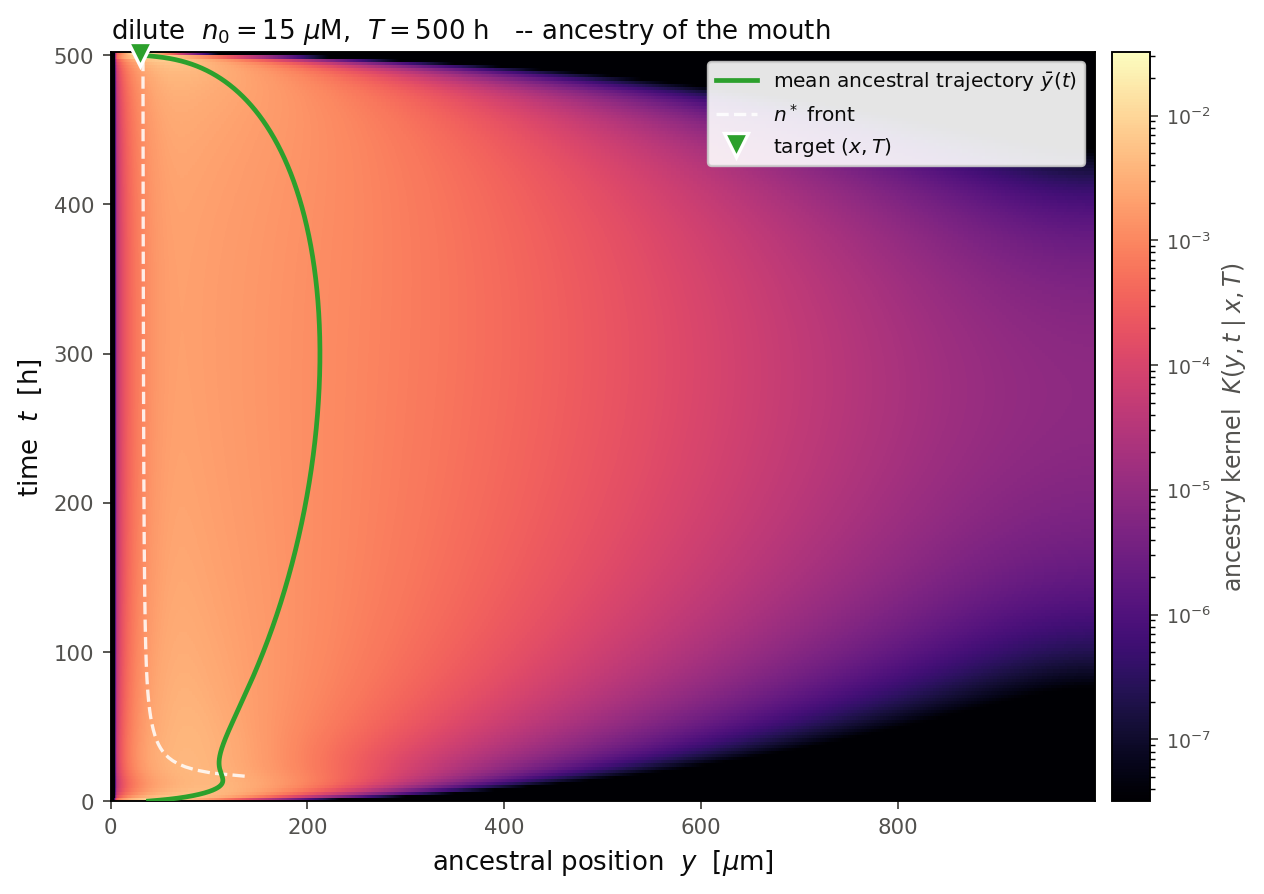
\includegraphics[width=\textwidth]{kerneldilutemouth}
			\caption{Dilute opening, $T=500h, n_0=15 \mathrm{\mu M}$}
			\label{fig:kerneldilm}
		\end{subfigure}
		\hfill
		\begin{subfigure}{0.45\textwidth}
			\centering
			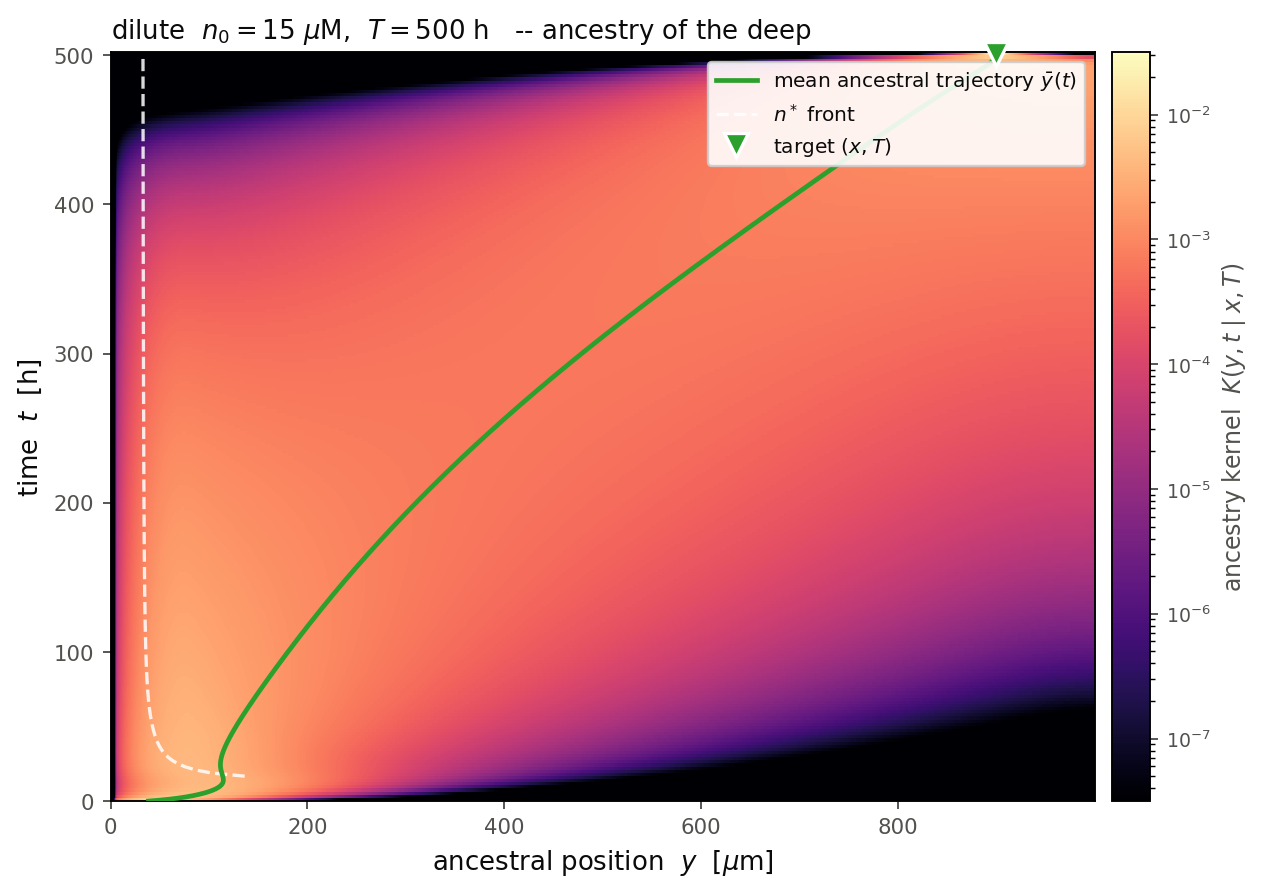
\includegraphics[width=\textwidth]{kerneldilutedeep}
			\caption{Dilute deep end, $T=500h, n_0=15 \mathrm{\mu M}$}
			\label{fig:kerneldildeep}
		\end{subfigure}
	\hfill
			\begin{subfigure}{0.45\textwidth}
		\centering
		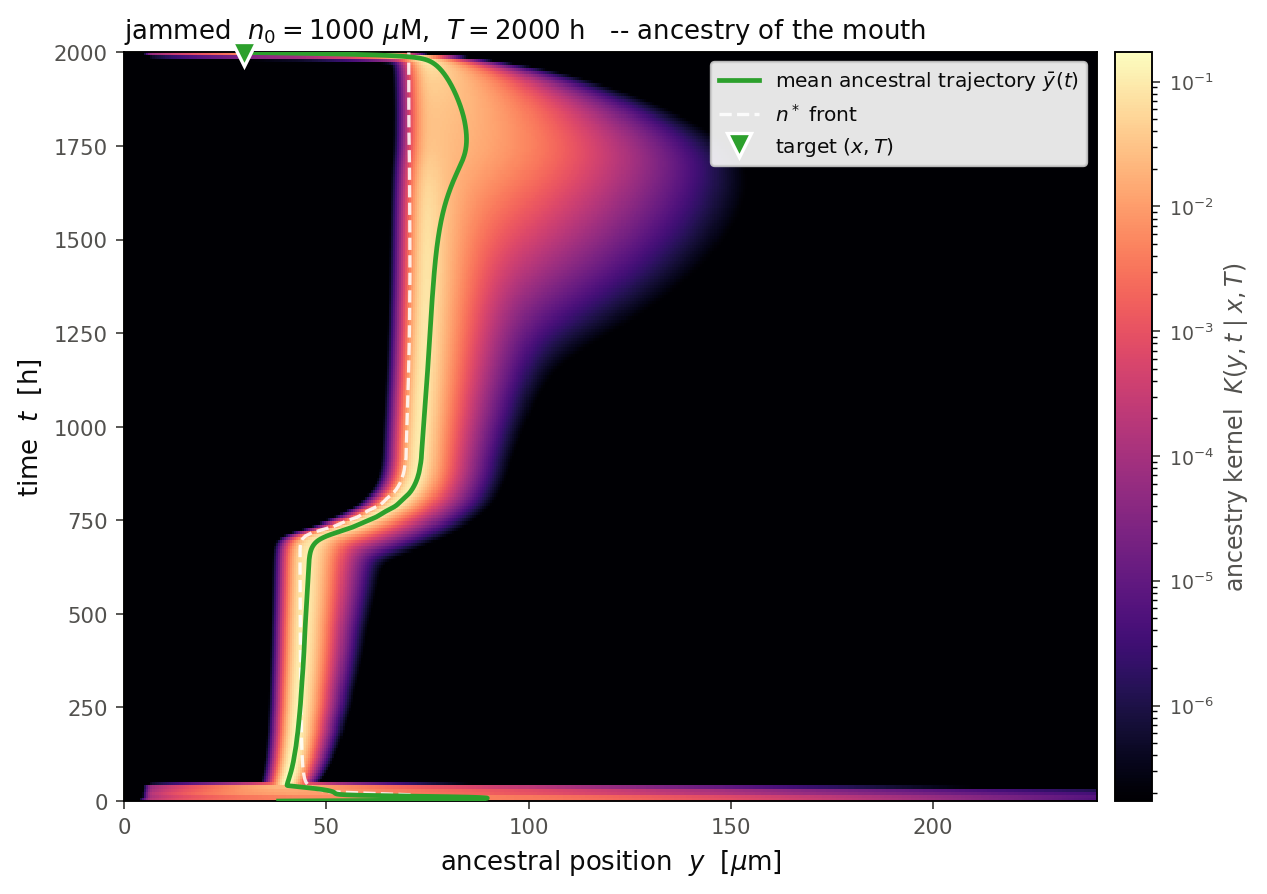
\includegraphics[width=\textwidth]{kerneljammouth}
		\caption{Jammed opening, $T=2000h, n_0=1000 \mathrm{\mu M}$}
		\label{fig:kerneljammouth}
	\end{subfigure}
	\hfill
	\begin{subfigure}{0.45\textwidth}
		\centering
		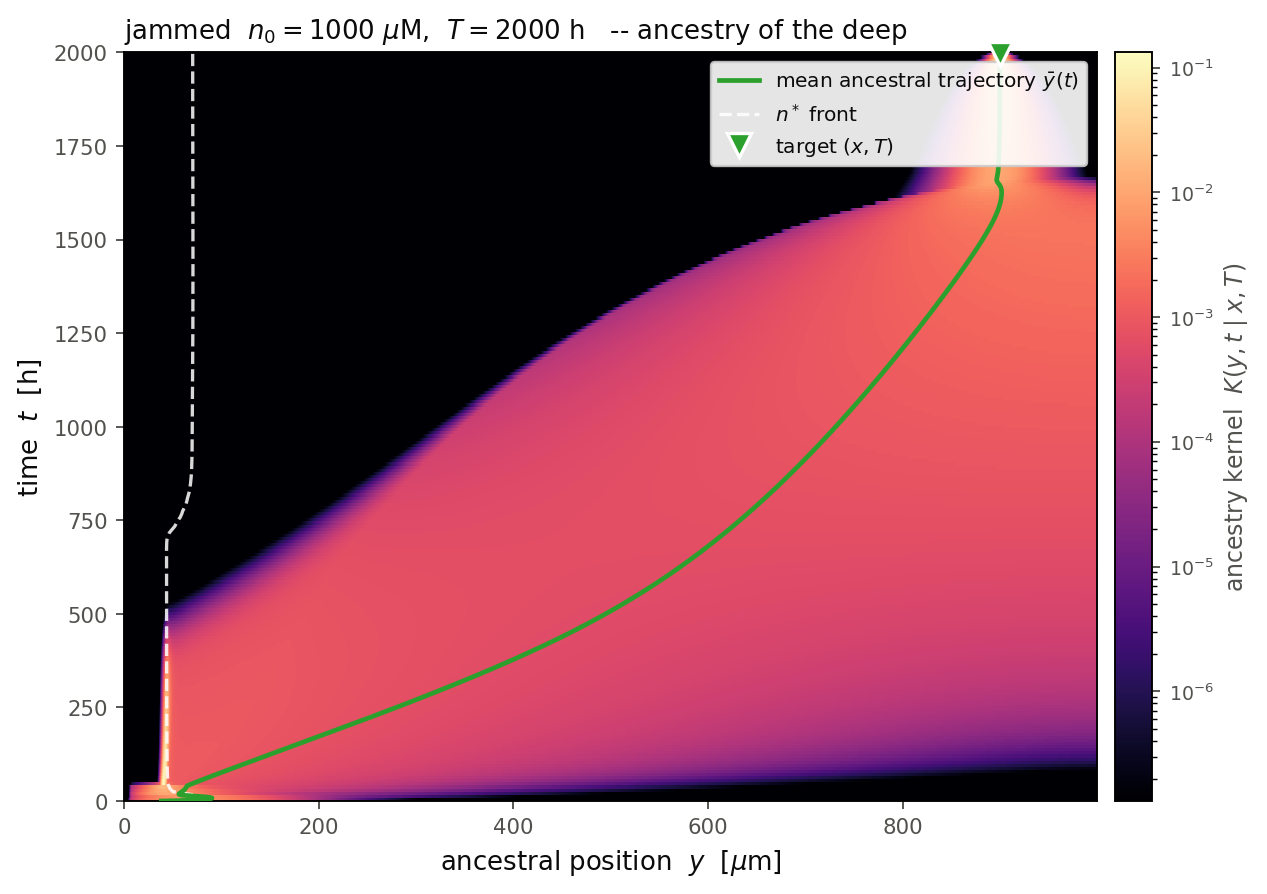
\includegraphics[width=\textwidth]{kerneljamdeep}
		\caption{Jammed deep end, $T=2000h, n_0=1000 \mathrm{\mu M}$}
		\label{fig:kerneljamdeep}
	\end{subfigure}
		\caption{Ancestry Kernel as a space-time heatmap, deterministic trajectory backwards in time for a final fixed point.}
	\end{figure}
	\label{fig:kernel}
	\FloatBarrier
	\section{Growth factor}
	\label{sec:factor}
	Without the growth factor, densities can climb above 1, they have different run times, but both runs have reached their biomass maximum by $T \approx 30h$. So the run time difference is irrelevant. Not only can it result in nonsensical densities, but as seen in the first figure \ref{fig:noq}, the density overshoot can itself result in the wrong dynamics with a dip trade-off at $x\approx 700$ at the strain 1 selection front $n^*$. So the absence of the growth factor $q$ at very high $n_0$ can not only result in wrong density numbers, but in turn the overshoot can result in different dynamics. These are old runs without the limiter and with a seed of $\rho_{\mathrm{seed}}=10^{-16}$, so these are illustrations of the now fixed problems.
	\begin{figure}[htbp]
		\centering
		\begin{subfigure}{0.45\textwidth}
			\centering
			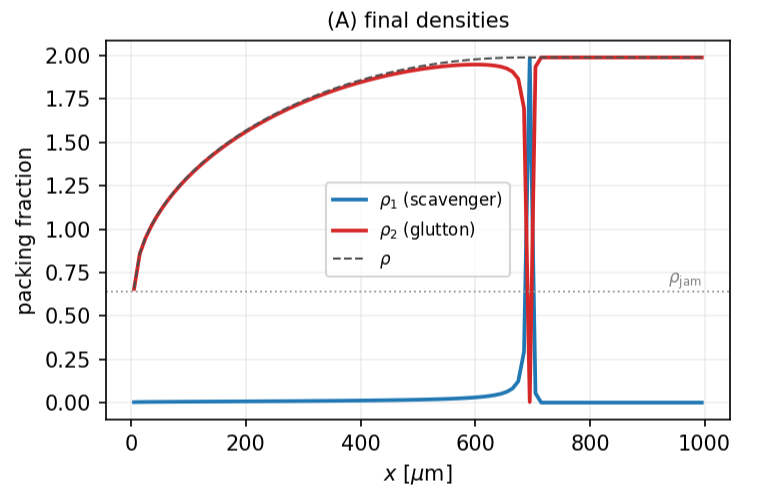
\includegraphics[width=\textwidth]{nogrowthfactor}
			\caption{Density without the growth factor, $n_0=10^6 \mathrm{\mu M}, T=6000h$}
			\label{fig:noq}
		\end{subfigure}
		\hfill
		\begin{subfigure}{0.45\textwidth}
			\centering
			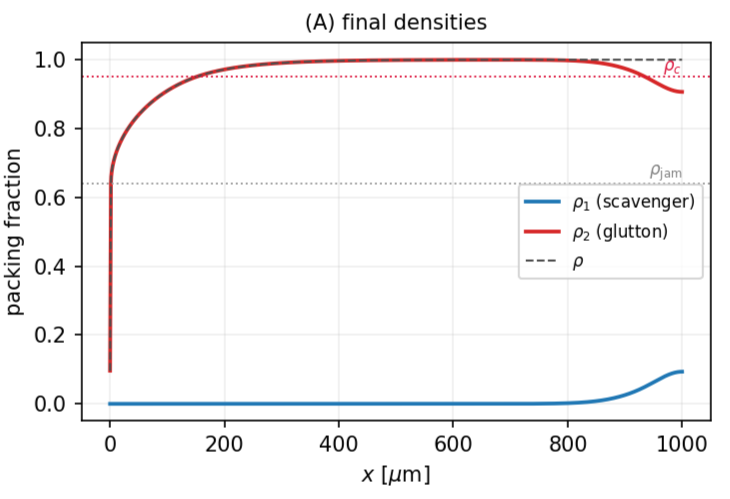
\includegraphics[width=\textwidth]{growthfactor}
			\caption{Growth factor $q$, $n_0=10^6 \mathrm{\mu M}, T=1000h$}
			\label{fig:q}
		\end{subfigure}
			\caption{Density comparison without and with the implemented growth factor}
\end{figure}
\label{fig:qfactor}
\section{Dilute limit}
\label{sec:dillimit}
\begin{figure}
	\centering
	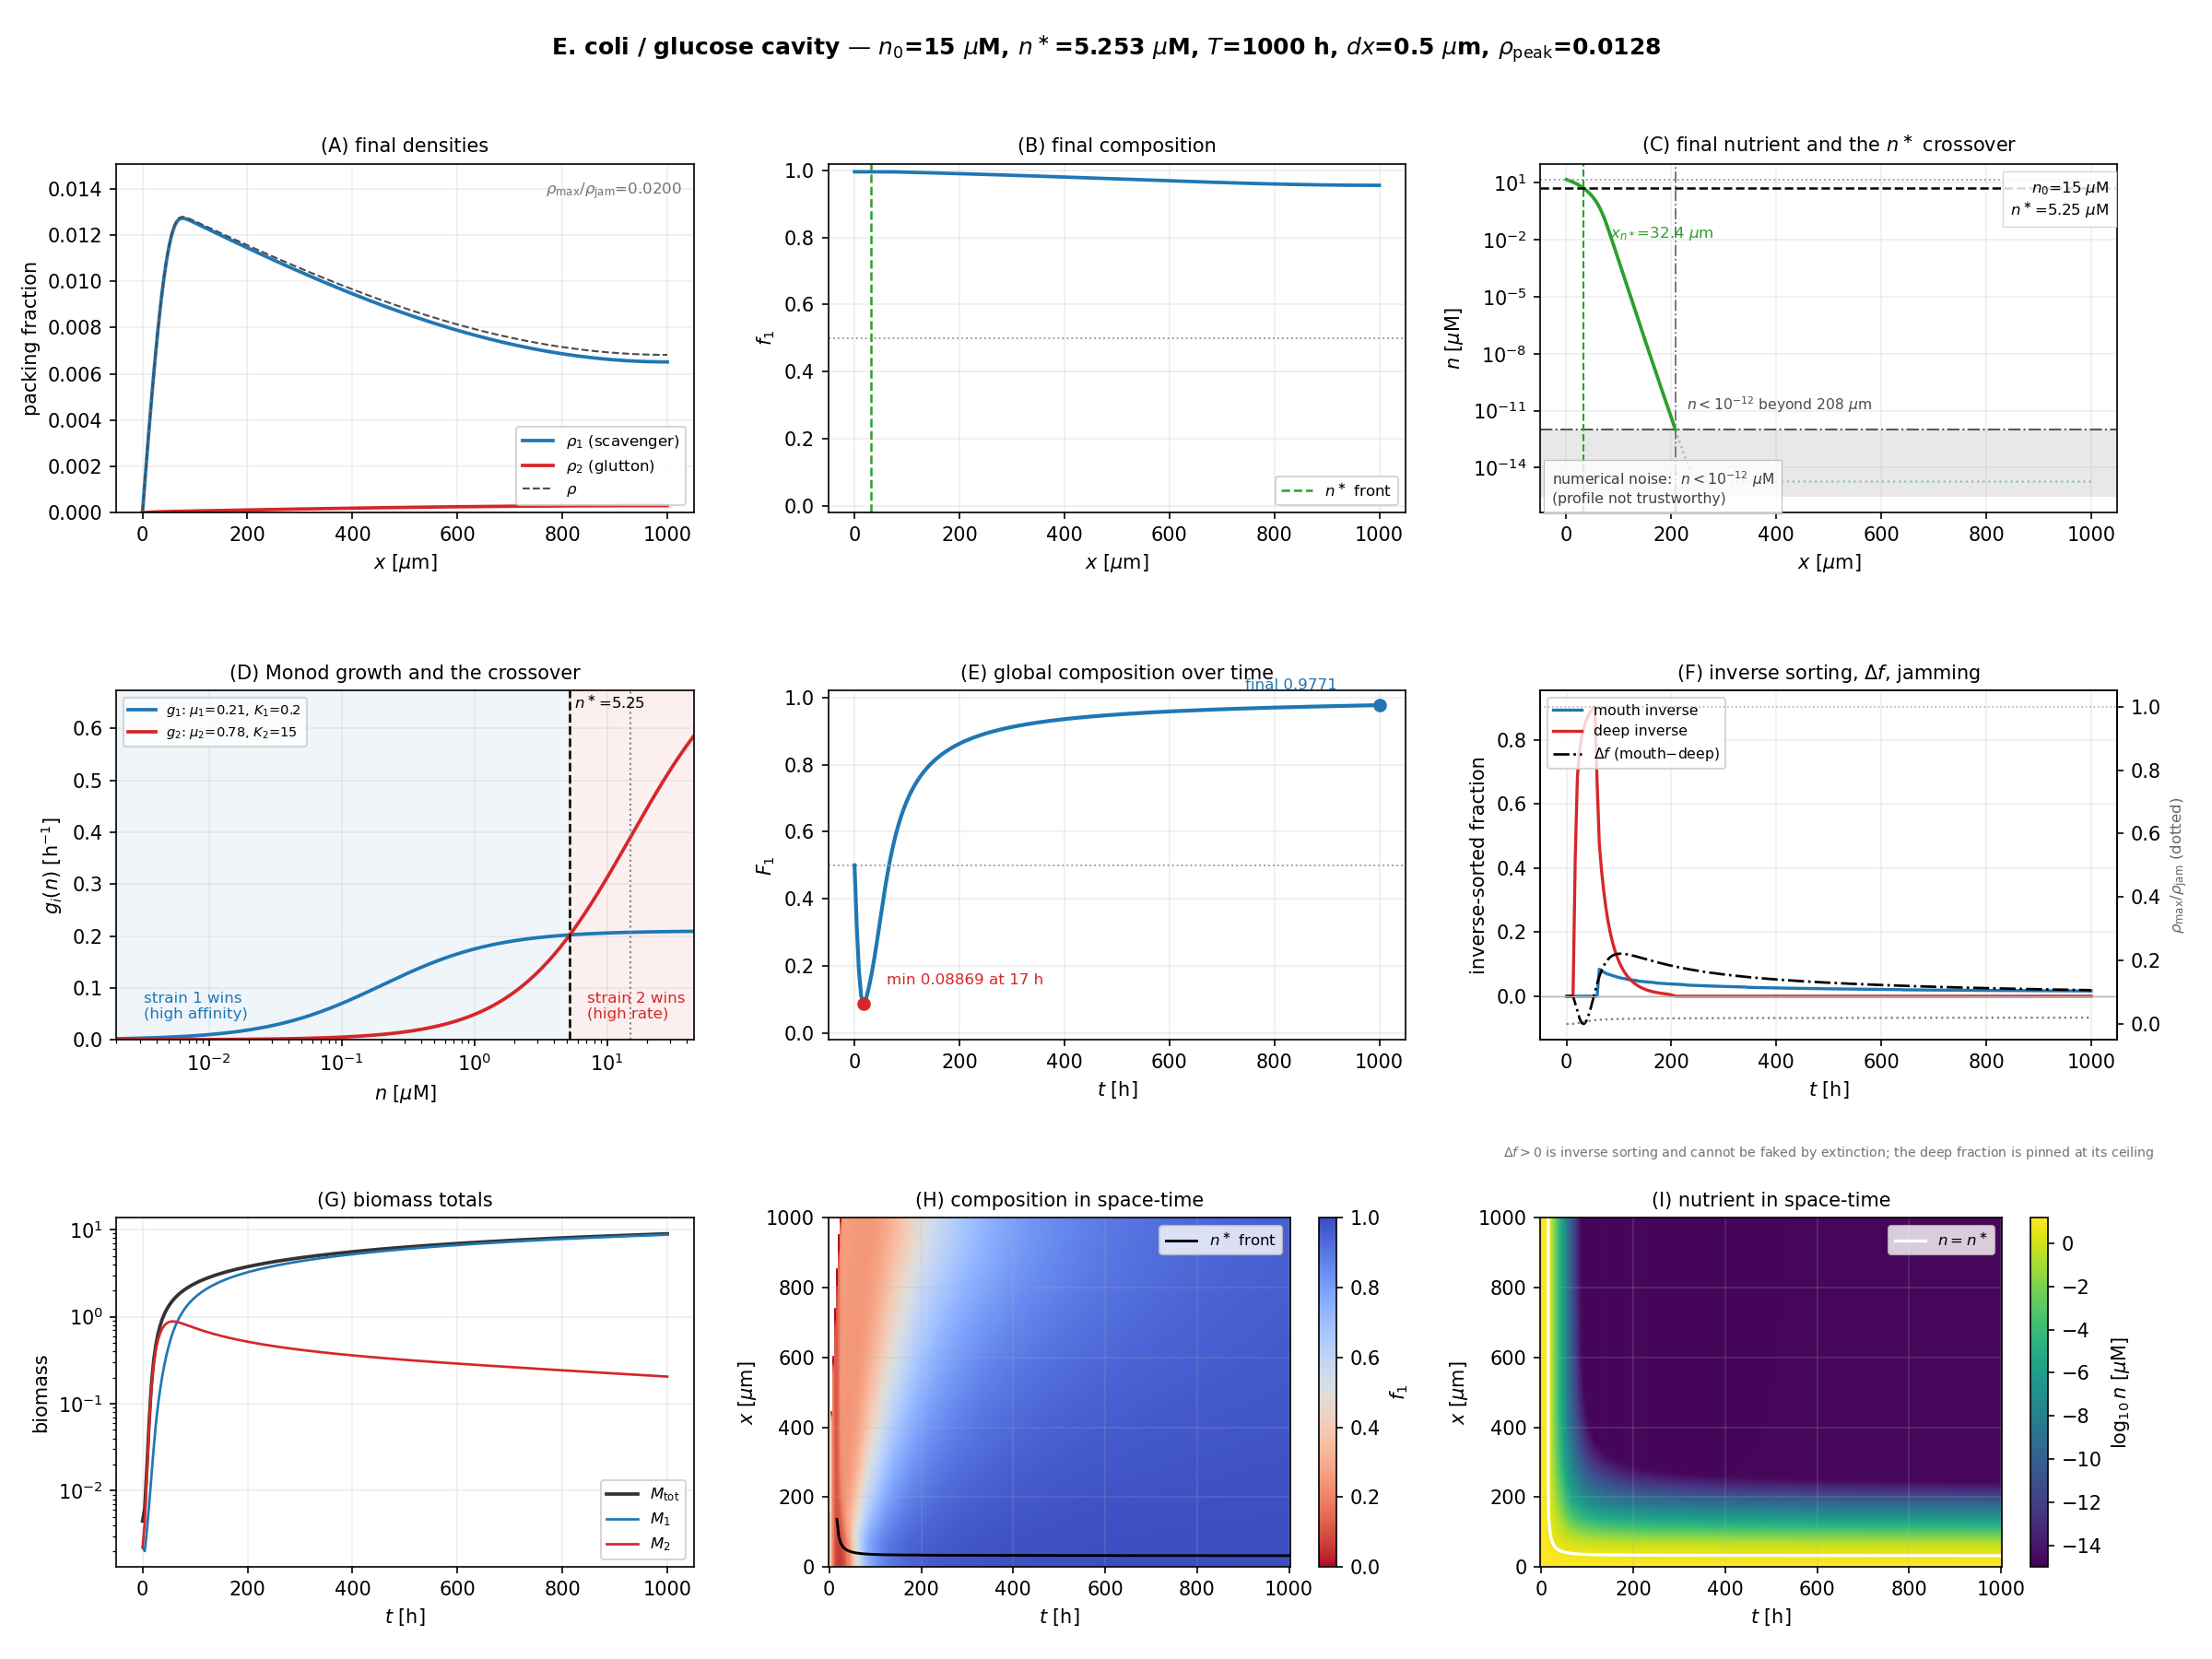
\includegraphics[width=\linewidth]{run_dil1000}
	\caption{Dilute run with T=1000h}
	\label{fig:rundil1000}
\end{figure}
Strain 2 decays exponentially and falls below one cell at $T=7986 h$ \ref{fig:rundildeath}, $F=1$ is globally satisfied.
\begin{figure}
	\centering
	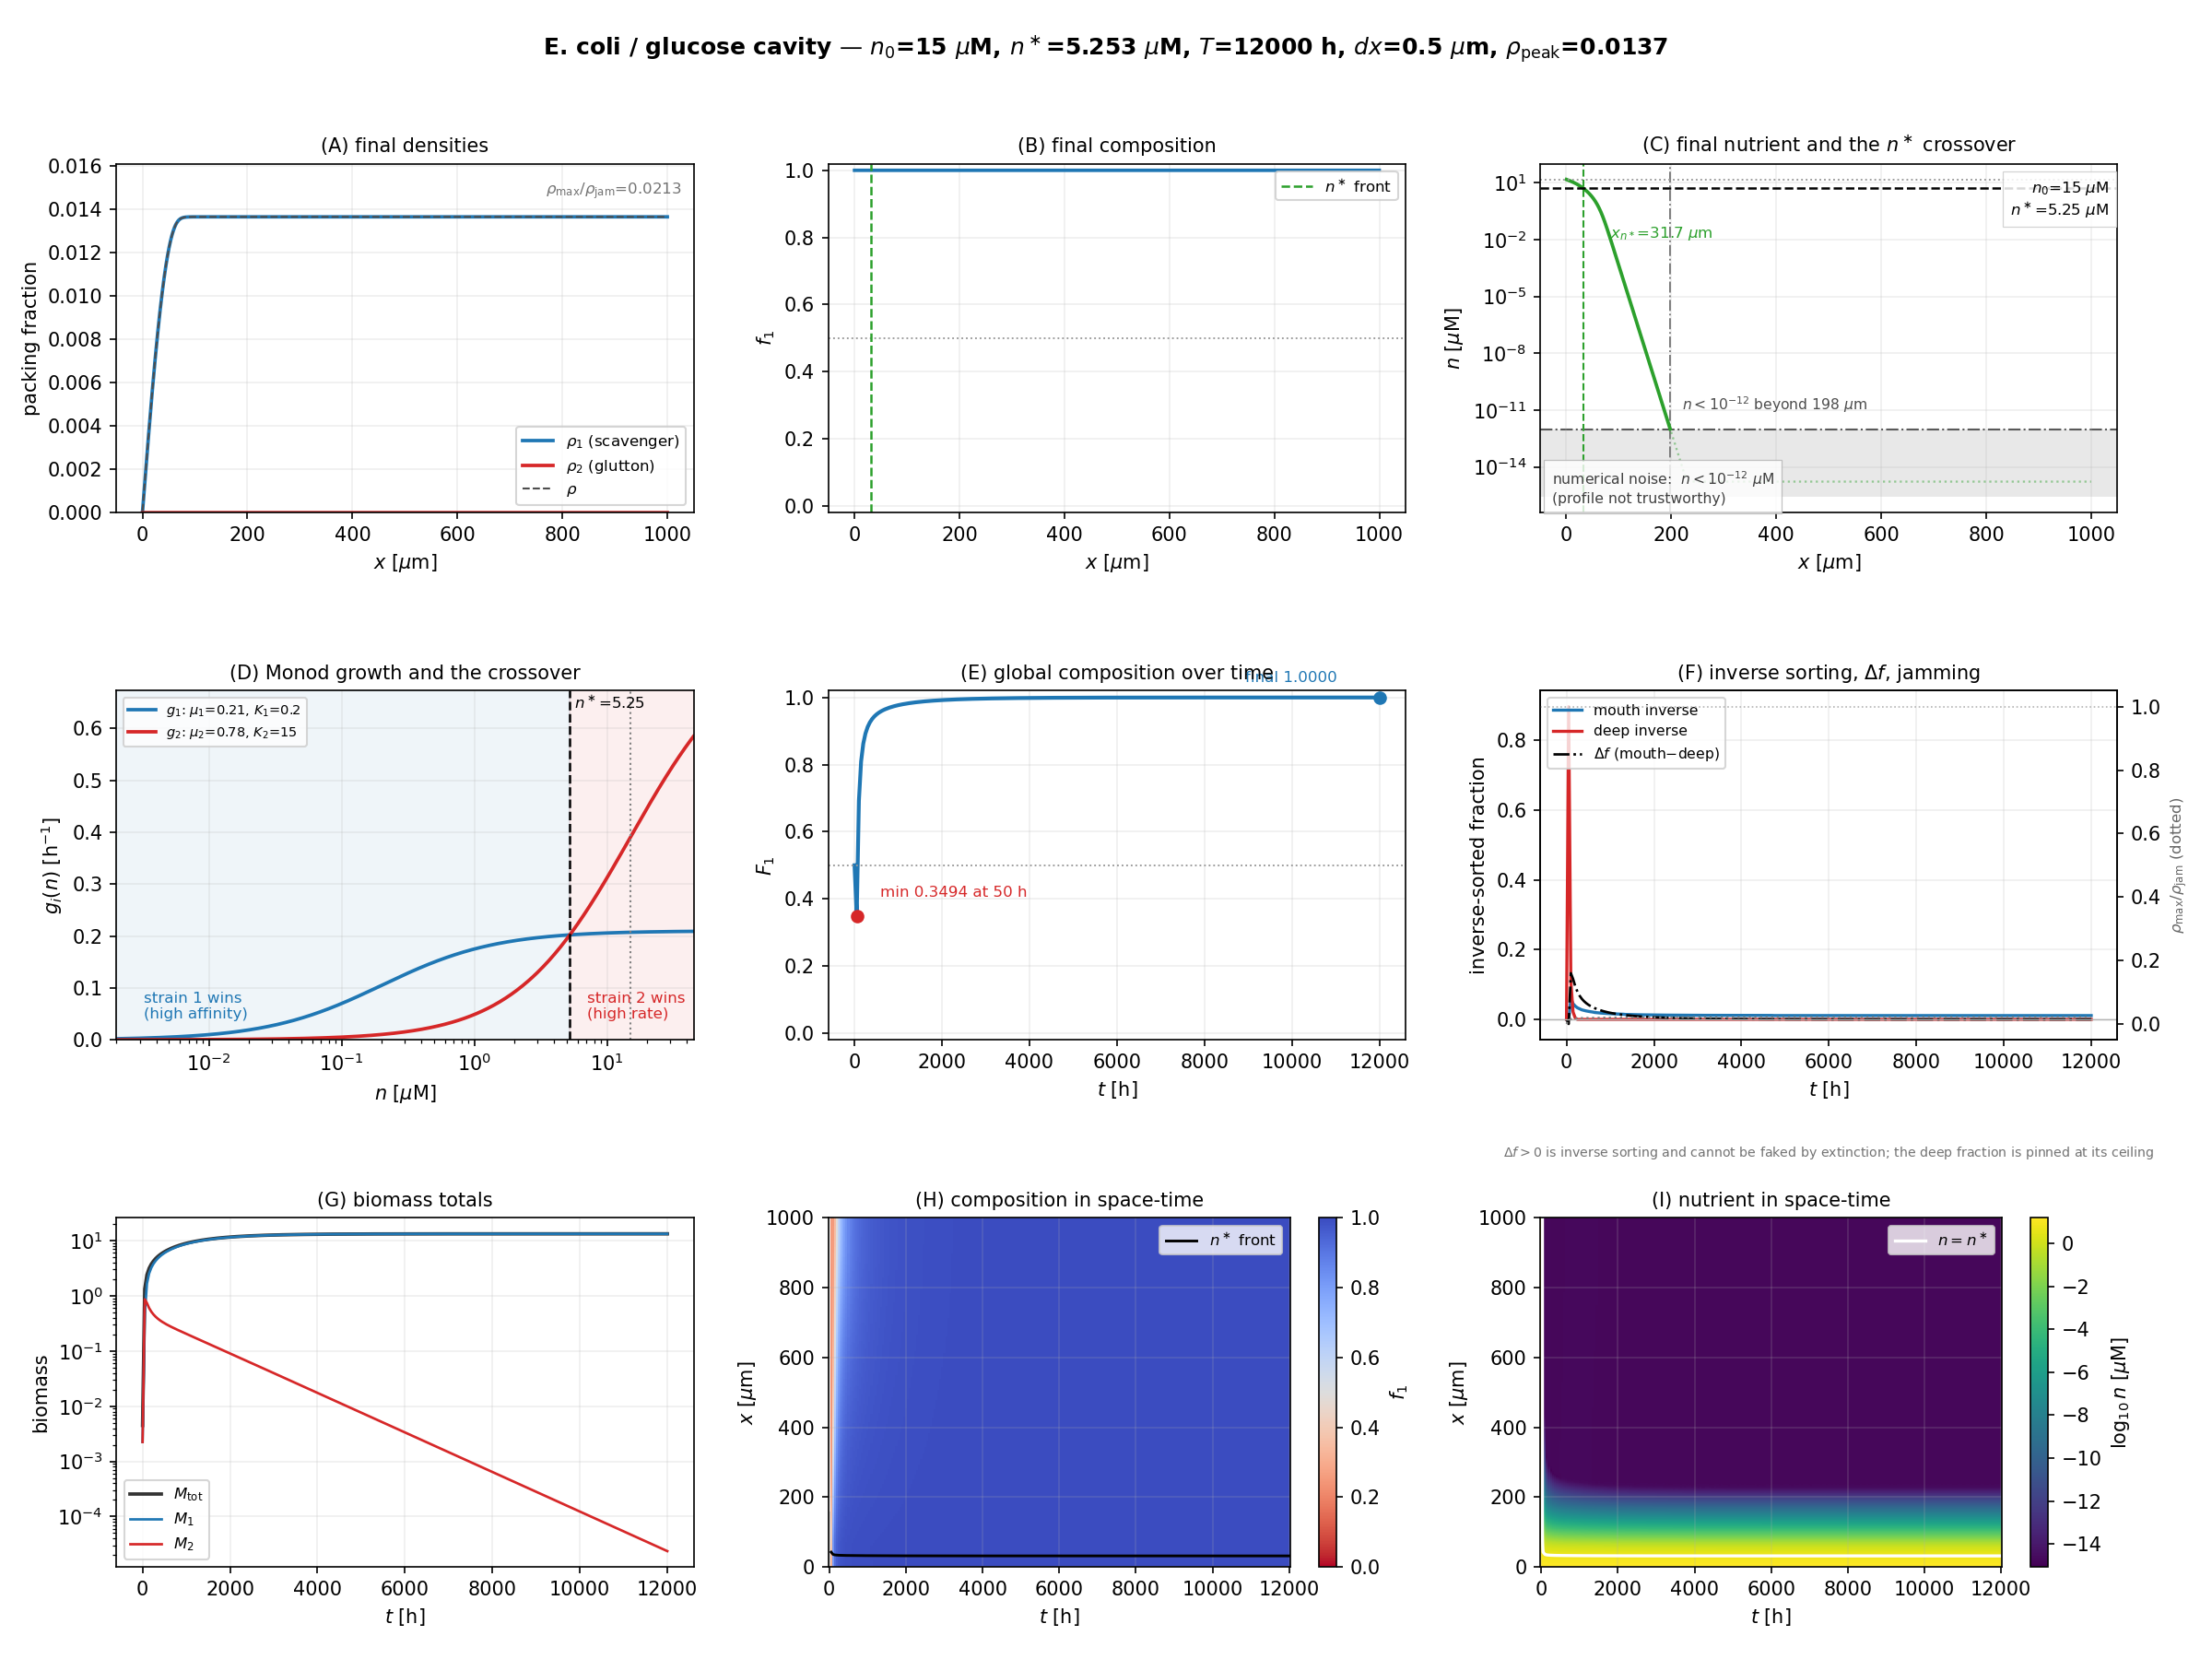
\includegraphics[width=\linewidth]{run_dildeath}
	\caption{Death of strain 2}
	\label{fig:rundildeath}
\end{figure}
\newpage
\section{Tilman: resource-ratio hypothesis}
\label{sec:rstar}
The resource-ratio hypothesis is for a well mixed chemostat, so not all requirements are fulfilled in our model \cite{rstar}. Yet in the dilute case, it still correctly predicts the competition result. $R^*$ is the minimum concentration of our resource (glucose) at which a strain can maintain a stable population, i.e. the growth rate is equal to the death rate. The only way for a cell to die in our model is to be washed out, so the death rate is the washout rate. We write the continuity equations per capita
\begin{equation}
	\frac{1}{\rho_i}\pd_t\rho_i
	=g_i(n)
	-\frac{1}{\rho_i}\pd_xJ_i,
	\qquad
	\pd_tn
	=D_n\pd_{xx}n
	-\frac1Y \bigl[g_1(n)\rho_1+g_2(n)\rho_2\bigr].
	\label{eq:tilman_in_our_variables}
\end{equation}
Tilmans assumption $\pd g_i/\pd \rho_j=0$ holds, because the strains only couple through
the nutrient. However the washout rate is not constant, like the mortality rate in Tilmans model \cite{rstar}.
\begin{equation}
	m_i(x,t):=\frac{1}{\rho_i}\pd_xJ_i,
	\label{eq:local_loss_rate}
\end{equation}
is the washout sink. Integrating biomass continuity equations over the cavity, using $J(L,t)=0$ and the biomass integral $M=\int_0^L\rho\dd x$ gives
\begin{equation}
	\frac{\dd M}{\dd t}=\int_0^L\bigl[g_1(n)\rho_1+g_2(n)\rho_2\bigr]\dd x+J(0,t),
	\label{eq:mass_budget}
\end{equation}
The loss through the opening is $-J(0,t)>0$. The uniform rate that
removes biomass per capita is 
\begin{equation}
	m^{\mathrm{eff}}:=-\frac{J(0,t)}{M},
	\label{eq:m_eff_flux}
	\end{equation}
at steady state (t $\rightarrow \infty$) $\dd M/\dd t=0$ , this is equal to the biomass weighted mean growth rate
\begin{equation}
	m^{\mathrm{eff}}
	=\frac{1}{M}\int_0^L\bigl[g_1(n)\rho_1+g_2(n)\rho_2\bigr]\dd x
	=\bigl\langle g\bigr\rangle_{\rho},
	\label{eq:m_eff_growth}
	\end{equation}
For the dilute cavity we use $n_0=15\,\mathrm{\mu M}$, $L=1000\,\mathrm{\mu m}$. From the \ref{fig:rundildeath} simulation we have $M=13.303619\,\mathrm{\mu m}$ and $J(0,T)=-0.1171732\mathrm{\frac{\mu m}{h}}$ at final time.

\begin{equation}
	g_i\bigl(R^{*}_i\bigr)=m^{\mathrm{eff}}.
	\label{eq:breakeven}
\end{equation}

\begin{equation}
	\frac{\mu_iR^{*}_i}{K_i+R^{*}_i}=m^{\mathrm{eff}}
	\;\Longrightarrow\;
	\mu_iR^{*}_i=m^{\mathrm{eff}}K_i+m^{\mathrm{eff}}R^{*}_i
	\;\Longrightarrow\;
	R^{*}_i\bigl(\mu_i-m^{\mathrm{eff}}\bigr)=m^{\mathrm{eff}}K_i .
	\label{eq:rstar_steps}
\end{equation}
\begin{equation}
	{\;R^{*}_i=\frac{K_i\,m^{\mathrm{eff}}}{\mu_i-m^{\mathrm{eff}}}\;},
	\qquad 0<m^{\mathrm{eff}}<\mu_i .
	\label{eq:rstar_monod}
\end{equation}
\begin{equation}
	R^{*}_1=8.76\times10^{-3}\,\mathrm{\mu M},
	\qquad
	R^{*}_2=1.71\times10^{-1}\,\mathrm{\mu M},
	\label{eq:rstar_cavity}
\end{equation}
so $R^{*}_1<R^{*}_2$. So the high affinity strain has the lower $R^*$ and therefore is expected to win by Tilmans prediction. Tilmans $R^*$ assumes a well mixed chemostat, using the total dilution rate rather than the individual one. Our cavity however is not well mixed, $m^{\mathrm{eff}}$ differs per strain: $m_1^{\mathrm{eff}} = 8.81 \times 10^{-3}, m_2^{\mathrm{eff}} = 2.23 \times 10^{-3}$, so the gluttons spatial refuge in the deep end results in a fourfold lower washout rate but loses anyway.

\end{document}
